\documentclass[a4paper,12pt,english,abstract=on,titlepage=false]{scrreprt}
\usepackage{setspace} %linespacing
\onehalfspacing
%\setlength{\parskip}{1em} % paragraph spacing
\usepackage[affil-it]{authblk}
\usepackage{graphicx}
\usepackage[space]{grffile}
\usepackage{latexsym}
\usepackage{textcomp}
\usepackage{longtable}
\renewcommand\floatpagefraction{0.1}
\usepackage{multirow,booktabs}
\usepackage{amsfonts,amsmath,amssymb}
\usepackage{gensymb}  % to show special symbols like degree °
\usepackage{url}
\usepackage{dcolumn} % needed for tables in chapter 5
%\usepackage[utf8]{inputenc}
\usepackage{hyperref}
\hypersetup{colorlinks=false,pdfborder={0 0 0}}
%\usepackage{latexml}
\newcommand{\truncateit}[1]{\truncate{0.8\textwidth}{#1}}
\newcommand{\scititle}[1]{\title[\truncateit{#1}]{#1}}
\usepackage{lmodern}
\usepackage[T1]{fontenc}
\usepackage[utf8]{inputenc}
\usepackage{geometry}
\geometry{verbose,tmargin=2cm,bmargin=2cm,lmargin=4cm,rmargin=2cm}
\providecommand{\tabularnewline}{\\}
\usepackage[printonlyused]{acronym}
%\usepackage[nolist]{acronym}
\usepackage{ltablex,array} % to scale longtables
\usepackage{lipsum}
\usepackage[flushleft]{threeparttable}  %adds notes to tables
\usepackage{etoolbox}% http://ctan.org/pkg/etoolbox
\appto\TPTnoteSettings{\footnotesize}
\usepackage{caption}

%fix problem with narrower table once using caption inside tabularx environment as suggested in last response here http://www.latex-community.org/forum/viewtopic.php?f=45&p=39951

\makeatletter
\patchcmd{\TX@endtabularx}% <cmd>
  {\def\caption}% <search>
  {\def\caption{\caption@withoptargs\TX@caption}%
   \def\TX@caption##1##2}% <replace>
  {}{}% <success><failure>
\makeatother


\usepackage{graphicx}
\usepackage[Export]{adjustbox}
%\newcommand{\sym}[1]{\ensuremath{^{#1}}} % for symbols in Table
%landscape pages
\usepackage{pdflscape}
\newcommand{\comment}[1]{}  %allows multiline comments
%\usepackage[english]{babel}% Recommended
%\usepackage{csquotes}
\usepackage[
maxcitenames=2, 
style=authoryear-comp,
firstinits=true,
maxbibnames=99,
backend=biber,
uniquename=false,
url=false,
doi=false,
isbn=false]{biblatex}
\DeclareNameAlias{sortname}{last-first}
\DeclareFieldFormat{pages}{#1}%
\renewcommand*{\nameyeardelim}{\addcomma\space} %adds comma between name and years in citations

\renewbibmacro{in:}{}
\renewbibmacro*{volume+number+eid}{%
  \printfield{volume}%
  \setunit*{\adddot}% DELETED
  \setunit*{\addnbspace}% NEW (optional); there's also \addnbthinspace
 \printfield{number}%
 \setunit{\addcomma\space}%
 \printfield{eid}}
\DeclareFieldFormat[article]{number}{\mkbibparens{#1}}
\DeclareLanguageMapping{english}{english-apa}  %needed for APA style
\AtEveryBibitem{
  \clearfield{labelmonth}
}

%patch fullcite command so that full citation in text is same as in references: http://tex.stackexchange.com/questions/43196/biblatex-fullcite-produces-different-result-from-bibliography-entry
\DeclareCiteCommand{\fullcite}
  {\usebibmacro{prenote}}
  {\usedriver
     {\defcounter{minnames}{6}%
      \defcounter{maxnames}{6}}
     {\thefield{entrytype}}.}
  {\multicitedelim}
  {\usebibmacro{postnote}}
\addbibresource{/home/till/Dokumente/BibTex/Second_Mexico_paper-Article.bib}
\addbibresource{/home/till/Dokumente/BibTex/Thesis.bib}
%\usepackage[authoryear]{natbib}

%\nobibliography*
% paper margins
\usepackage{geometry}
\geometry{
letterpaper,
left=25mm,
right=30mm,
top=20mm,
bottom=30mm,
}   
%limiting tables to only float within section
\usepackage[section]{placeins}
  
%use for commands only working with pdf
  


% *****************************************************************
% siunitx
% *****************************************************************
\usepackage{siunitx} % centering in tables
	\sisetup{
		detect-mode,
		tight-spacing		= true,
		group-digits		= false ,
		input-signs		= ,
		input-symbols		= ( ) [ ] - + *,
		input-open-uncertainty	= ,
		input-close-uncertainty	= ,
		table-align-text-post	= false
        }



%For tables commands, especially tabularx
\newcolumntype{b}{X}  %large columns http://tex.stackexchange.com/questions/84400/table-layout-with-tabularx-column-widths-502525
\newcolumntype{m}{>{\hsize=.5\hsize}X} % medium columns
\newcommand{\merge}[1]{\multicolumn{2}{>{\hsize=\dimexpr2\hsize+2\tabcolsep+\arrayrulewidth\relax}X}{#1}}  %allows merging of two columns in tabularx http://tex.stackexchange.com/questions/236155/tabularx-and-multicolumn

\newcolumntype{Y}{>{\centering\arraybackslash}X} %new columntype for X columns in tabularx to center them http://tex.stackexchange.com/questions/89166/centering-in-tabularx-and-x-columns
\newcolumntype{Z}{>{\raggedright\let\newline\\\arraybackslash\hspace{0pt}}X} %left aligned X columns http://tex.stackexchange.com/questions/97180/how-to-get-column-alignment-in-tabularx
\newcolumntype{z}{>{\hsize=.5\hsize\\\raggedright\let\newline\\\arraybackslash\hspace{0pt}}X} %left aligned X columns http://tex.stackexchange.com/questions/97180/how-to-get-column-alignment-in-tabularx
\newcolumntype{y}{>{\hsize=.5\hsize}Y} % small columns

%DIF LATEXDIFF DIFFERENCE FILE
%DIF DEL Before_corrections/Thesis.tex   Mon Sep 26 15:58:29 2016
%DIF ADD Thesis.tex                      Wed Feb 15 08:58:31 2017
%DIF PREAMBLE EXTENSION ADDED BY LATEXDIFF
%DIF UNDERLINE PREAMBLE %DIF PREAMBLE
\RequirePackage[normalem]{ulem} %DIF PREAMBLE
\RequirePackage{color}\definecolor{RED}{rgb}{1,0,0}\definecolor{BLUE}{rgb}{0,0,1} %DIF PREAMBLE
\providecommand{\DIFadd}[1]{{\protect\color{blue}\uwave{#1}}} %DIF PREAMBLE
\providecommand{\DIFdel}[1]{{\protect\color{red}\sout{#1}}}                      %DIF PREAMBLE
%DIF SAFE PREAMBLE %DIF PREAMBLE
\providecommand{\DIFaddbegin}{} %DIF PREAMBLE
\providecommand{\DIFaddend}{} %DIF PREAMBLE
\providecommand{\DIFdelbegin}{} %DIF PREAMBLE
\providecommand{\DIFdelend}{} %DIF PREAMBLE
%DIF FLOATSAFE PREAMBLE %DIF PREAMBLE
\providecommand{\DIFaddFL}[1]{\DIFadd{#1}} %DIF PREAMBLE
\providecommand{\DIFdelFL}[1]{\DIFdel{#1}} %DIF PREAMBLE
\providecommand{\DIFaddbeginFL}{} %DIF PREAMBLE
\providecommand{\DIFaddendFL}{} %DIF PREAMBLE
\providecommand{\DIFdelbeginFL}{} %DIF PREAMBLE
\providecommand{\DIFdelendFL}{} %DIF PREAMBLE
%DIF END PREAMBLE EXTENSION ADDED BY LATEXDIFF

\begin{document}
%\begin{acronym}
\acro{2SLS} {two-stage least squares}
\acro{ATE} {average treatment effect}
\acro{ATT} {average treatment effect on the treated}
\acro{AUD} {Australian Dollar}
\acro{BLUE} {best linear unbiased estimator}
\acro{BMI} {body mass index}  
\acro{BP} {bivariate probit}
\acro{CHNS} {China Health and Nutrition Survey}
\acro{COI} {cost-of-illness} 
\acro{DALYs} {disability-adjusted life years}
\acro{EUR} {Europe}
\acro{ENSA} {La Encuesta Nacional de Salud}
\acro{FE} {fixed effects}  
\acro{ENSANUT}{Encuesta Nacional de Salud y Nutricion}
\acro{FGLS} {Feasible General Least Squares}
\acro{GDP} {gross-domestic-product} 
\acro{HbA1c} {glycated hemoglobin}  
\acro{HIC} {high-income country} 
\acro{ICD}{International Statistical Classification of Diseases and Related Health Problems}
\acro{IDF} {International Diabetes Federation}
\acro{INEGI} {Instituto Nacional de Estadistica y Geografia} 
\acro{IV} {instrumental variable}
\acro{LATE} {local average treatment effect}
\acro{LIC} {low-income country} 
\acro{LMIC} {low- and middle-income country} 
\acro{LPM} {linear probability model}
\acro{MSM} {marginal structural model} 
\acro{MENA} {Middle East and North Africa}
\acro{MIC} {middle-income country}  
\acro{MxFLS} {Mexican Family Life Survey}
\acro{NAC} {North American and Caribbean}
\acro{NCD} {non-communicable disease}
\acro{OLS} {ordinary least squares}
\acro{OOP} {out-of-pocket}   
\acro{PML} {pseudo-maximum-likelihood}
\acro{p.p.} {percentage points}
\acro{PPP}{purchasing-power-parity}
\acro{PRISMA} {Preferred Reporting Items for Systematic Reviews and Meta-Analyses}
\acro{RE} {random effects}
\acro{SACA} {South and Central America}
\acro{SEA} {South East Asia}
\acro{SSA} {Sub-Saharan Africa}
\acro{UK} {United Kingdom}
\acro{WHO} {World Health Organization}
\acro{WP} {Western Pacific}
\acro{WTP} {willingness to pay
}    

\end{acronym}

\acrodefplural{LMIC}[LMICs]{low- and middle-income countries}  

\acrodefplural{HIC}[HICs]{high-income countries}

\acrodefplural{MIC}[MICs]{middle-income countries}
 
\acrodefplural{LIC}[LICs]{low-income countries} 
% Title Page
%\comment{
\date{\today}
\makeatletter
\begin{titlepage}
\centering
\vfill
Thesis submitted for the degree of Doctor of Philosophy (PhD)
\par
\vspace*{1in}
\begin{Large}\bfseries
The Economics of Type 2 Diabetes in Middle-Income Countries\par
\end{Large}
\vspace{1in}
\begin{large}\bfseries
Till Seuring\par
\end{large}
\par
\vspace{0.2in}
Norwich Medical School
\par
University of East Anglia, UK
\par
\vspace{1.0in}
September 2016
\par
\vspace{2.0in}
This copy of the thesis has been supplied on condition that anyone who consults it is
understood to recognise that its copyright rests with the author and that use of any
information derived there from must be in accordance with current UK Copyright Law.
In addition, any quotation or extract must include full attribution.
\end{titlepage}
\makeatother

\cleardoublepage
\addcontentsline{toc}{chapter}{\nameref{abstract}}
\chapter*{\label{abstract}Abstract}
This thesis researches the economics of type 2 diabetes in \acfp{MIC}. Given its rising prevalence, in-depth country specific analysis is key for understanding the economic consequences of type 2 diabetes in \acp{MIC}. It analyses the economic burden of type 2 diabetes in terms of labour market consequences, taking into account the heterogeneity of the diabetes population, for both Mexico and China. For China, also evidence on the effects of a diabetes diagnosis on health behaviours is provided.

The thesis consists of four studies with the unifying theme of improving our understanding of the causal impact of diabetes on  economic outcomes. Study (1) provides an updated overview, critically assesses and identifies gaps in the current literature on the economic costs of type 2 diabetes using a systematic review approach; study (2) investigates the effects of self-reported diabetes on employment probabilities in Mexico, using cross-sectional data and making use of a commonly used \acf{IV} approach; study (3) revisits and extends these results via the use of \ac{FE} panel data analysis, also considering a broader range of outcomes, including wages and working hours. Further, it makes use of cross-sectional biomarker data that allow for the investigation of measurement error in self-reported diabetes. Study (4) researches the effect of a diabetes diagnosis on employment as well as behavioural risk factors in China, using longitudinal data and applying an alternative identification strategy, \acf{MSM} estimation, while comparing these results with \ac{FE} estimation results.\footnote{Chapters \ref{cha:review} and \ref{cha:Mex1} have appeared as journal articles in \textit{PharmacoEconomics} and \textit{Economics \& Human Biology}, respectively. Chapter \ref{cha:Mex2} has appeared as a working paper and been submitted for publication. For further details see page \pageref{publication_statement}.}

The findings of the first paper document a considerable increase in studies on the economic costs of diabetes in \acp{MIC}. It also illustrates that most of the evidence is based on cost-of-illness studies and the literature on adverse labour market effects of diabetes in \acp{MIC} is scarce. The thesis fills part of this void and shows that self-reported diabetes has a considerable impact on employment probabilities of people living in Mexico. The findings are robust to the application of different estimation strategies. No consistent evidence of an adverse effect of diabetes on wages or working hours is found. The findings for Mexico in the second and third paper suggest considerable inequities in the adverse labour market effects of diabetes, as it mainly affects the poor, less protected as well as women. Taking into account those unaware of the disease, the adverse effect of diabetes is reduced because undiagnosed diabetes itself does not show an adverse association with any labour market outcome. This suggests that the undiagnosed population is distinctly different from the diagnosed population, likely due to differences in health status and health information. The results from the fourth paper display strong discrepancies in the effect of diabetes on both employment probabilities and behavioural risk factors. For men, employment appears not to be affected by the diagnosis and they are able to reduce their levels of \ac{BMI}, waist circumference, alcohol and caloric consumption. Women, however, experience important reductions in employment probabilities and less favourable post-diagnosis changes in behavioural risk factors compared to men. These sex differences in risk factor reductions may provide an explanation for the more adverse employment effects for women. Importantly, accounting for confounding appears to be of particular importance when estimating the effects of a diagnosis on \ac{BMI} and waist circumference.

To reduce the economic burden, the groups most affected by the identified inequities should be targeted. Further, the underlying reasons for the found sex differences need to be identified.



\tableofcontents

\cleardoublepage
% \phantomsection
\addcontentsline{toc}{chapter}{\listfigurename}
\listoffigures

\cleardoublepage
% \phantomsection
\addcontentsline{toc}{chapter}{\listtablename} 
\listoftables
\cleardoublepage

\addcontentsline{toc}{chapter}{\nameref{publication_statement}}
\chapter*{\label{publication_statement}Publications and statement of authorship}


The research reported is my own original work which was carried out in collaboration with
others as follows:

\paragraph{Chapter \ref{cha:intro}:} Written by Till Seuring. 

\paragraph{Chapter \ref{cha:review}:} Till Seuring was the lead author of a paper published as:
\\[12pt]
\noindent\fullcite{Seuring2015a}
\\[12pt]
\noindent Till Seuring, Marc Suhrcke and Olga Archangelidi designed the study. The search strategy was designed and executed by Till Seuring. Till Seuring and Olga Archangelidi screened the initial results and extracted the data from the primary studies. Till Seuring drafted the original manuscript which was critically reviewed by Olga Archangelidi and Marc Suhrcke.

\paragraph{Chapter \ref{cha:Mex1}:} Till Seuring was the lead author of a paper published as:
\\[12pt]
\noindent\fullcite{Seuring2015}
\\[12pt]
\noindent Till Seuring, Yevgeniy Goryakin and Marc Suhrcke  designed the study. Till Seuring analysed the data. Till Seuring drafted the original manuscript which was critically reviewed by Yevgeniy Goryakin and Marc Suhrcke.


\paragraph{Chapter \ref{cha:Mex2}:} Till Seuring was the lead author of a working paper published as: 
Seuring T., Serneels P., Surcke, M. (2016), ``The impact of diabetes on labour market outcomes in Mexico: a panel and biomarker data analysis.'' It has appeared as \textit{IZA Discussion Paper} 10123, and \textit{York University Centre for Health Economics Research Paper 134}, and has been submitted for publication.

Till Seuring, Pieter Serneels and Marc Suhrcke designed the study. Till Seuring analysed the data. Till Seuring drafted the original manuscript which was critically reviewed by Pieter Serneels and Marc Suhrcke.



\paragraph{Chapter \ref{cha:China}:} Till Seuring and Max Bachmann designed the study. Till Seuring analysed the data. Till Seuring drafted the original manuscript which was critically reviewed by Max Bachmann and Pieter Serneels.

\paragraph{Chapter \ref{cha:Discussion}:} Written by Till Seuring.
\cleardoublepage

\addcontentsline{toc}{chapter}{\nameref{acknowledgements}}
\chapter*{\label{acknowledgements}Acknowledgements}

Being able to write these lines today, at the end of my PhD, is the culmination of a lot of luck I have had in my life. I have been so lucky to be able to live a life of my own choosing that allows me to pursue my goals, to embark on new adventures and to be surrounded by those great people without whom this thesis would not have been possible. 

First of all, I am grateful for my the best supervisory team there is. I never would have thought that I would have the opportunity to work with such kind and bright people. Thank you Marc. Without you I may never would have pursued a PhD nor would I have found my way to UEA. It was in Dubai \DIFdelbegin \DIFdel{were }\DIFdelend \DIFaddbegin \DIFadd{where }\DIFaddend we first met after I had attended your talk at the International Diabetes Congress, organized by my then employer. I asked you a couple of questions after your talk and we continued to chat for a few minutes afterwards and exchanged contact details. A few months later I contacted you regarding a PhD post at Cambridge, where you were involved in, and after some forth and back it became clear that there could be the opportunity to do a PhD with you at UEA. So it came that half a year later me and my wife actually moved to the fine city of Norwich and I would start a PhD. From then on it has been a great experience with a lot of work, but also a lot of fun. Thank you for always being responsive and helpful, interested in my work, providing great feedback and not hesitating one second to also support me from afar. The same has to be said of Pieter and Max, who became part of the supervisory team more or less at the midpoint of the PhD. Thank you Pieter for always pushing me to make my work better, for providing me with new ideas and for always being there when I had a question. I also enjoyed finding some common ground with you regarding the experience of being married to a women from Latin America. Thank you Max for being a just as great primary supervisor as Marc had been before going to York, for being so enthusiastic, for introducing me to the world of epidemiology and for taking time out of your busy schedule to sit down with me for several hours to go through Stata code. Of course I also have to thank Olia and Yevgeniy for being such great co-authors on my first two papers.

Then there is Katey	 to who I am deeply indebted. I am so grateful that you provided me a home in Norwich and I thoroughly enjoyed going to the pub, or watching the possibly worst movie ever, with you and Gareth. I also want to thank Darren for being a good friend every time I came to Norwich. 

Being surrounded only by PhD students (in Norwich) or nobody who had a clue of what I was actually doing (back home), was not always easy. Therefore, I am happy to count on a number of friends that provided just the right mix of both worlds. In no particular order, I am especially grateful to Heiner for organizing the two-men conference in Kijkduin\footnote{See also \textcite{Schmittdiel2016}.} and for joining in on many similar events; to Christian for keeping me up to date on the latest political chatter in the German development sphere; to Alex for always keeping his doors in Moabit open for me; and to Frank for just being the lifelong friend everybody needs.

I cannot forget the Big D. You are one of the main reasons I am doing what I do. You came into my life unannounced and uninvited and I had to learn to live with you because you left me no choice. I can only be thankful to be born a part of the world where dealing with you is difficult but doable, which allows me to live a ``normal'' life. Despite all the hard times you have given me, I am weirdly grateful that you handed me that personal invitation to pursue you in my research.  I hope that this thesis might be a small step towards a future where one day every person being affected by you will have the same possibilities I have had.

Of course this thesis would not have been possible without the best family in the world. Thank you Martin and Angelica for being the best \textit{suegros} and Annia for being the best \textit{cu\~{n}ada} I could have asked for. There is also my extended Mexican family, especially Wendy and Javier, which I am so happy to have. Being able to step into another world when visiting you is a blessing. It has given me much needed breaks from the life of a PhD student and being driven across Puebla to eat the best \textit{gorditas} with \textit{salsa verde con pipicha} is a very special treat. 

Also my two sisters, Anne and Elena, need to be mentioned. I am very fortunate to not only have such great sisters but to also be able to call you my friends. 
To my parents Martin and Petra: You are the reason that I am walking the face of this earth and have the chance to live this great life. Ich bin sehr glücklich Euch zu haben. Last, but certainly not least, a few words to my beautiful wife Ada and to my adorable little daughter Matilda who have been incredibly supportive even though they sometimes barely saw me during the final stages of this endeavour: Ich kann schwer beschreiben, wie sehr ich Euch liebe. Ihr seid das Beste in meinem Leben und mein größter Schatz. Las amo!

\cleardoublepage
\addcontentsline{toc}{chapter}{\nameref{abbreviations}}
\chapter*{\label{abbreviations}Abbreviations}

\begin{acronym}
\acro{2SLS} {two-stage least squares}
\acro{ATE} {average treatment effect}
\acro{ATT} {average treatment effect on the treated}
\acro{AUD} {Australian Dollar}
\acro{BLUE} {best linear unbiased estimator}
\acro{BMI} {body mass index}  
\acro{BP} {bivariate probit}
\acro{CHNS} {China Health and Nutrition Survey}
\acro{CHARLS} {The China Health and Retirement Longitudinal Study}
\acro{COI} {cost-of-illness} 
\acro{DAG} {direct acyclic graph}
\acro{DALYs} {disability-adjusted life years}
\acro{EUR} {Europe}
\acro{ENSA} {La Encuesta Nacional de Salud}
\acro{FE} {fixed effects}  
\acro{ENSANUT}{Encuesta Nacional de Salud y Nutricion}
\acro{FGLS} {Feasible General Least Squares}
\acro{GDP} {gross-domestic-product} 
\acro{HbA1c} {glycated hemoglobin}  
\acro{HIC} {high-income country} 
\acro{ICD}{International Statistical Classification of Diseases and Related Health Problems}
\acro{IDF} {International Diabetes Federation}
\acro{INEGI} {Instituto Nacional de Estadistica y Geografia} 
\acro{IV} {instrumental variable}
\DIFaddbegin \acro{IPTW}{inverse probability of treatment weights}
\DIFaddend \acro{LATE} {local average treatment effect}
\acro{LIC} {low-income country} 
\acro{LMIC} {low- and middle-income country} 
\acro{LPM} {linear probability model}
\acro{MSM} {marginal structural model} 
\acro{MENA} {Middle East and North Africa}
\acro{MIC} {middle-income country}  
\acro{MxFLS} {Mexican Family Life Survey}
\acro{NAC} {North American and Caribbean}
\acro{NCD} {non-communicable disease}
\acro{OLS} {ordinary least squares}
\acro{OOP} {out-of-pocket}   
\acro{PML} {pseudo-maximum-likelihood}
\acro{PPP}{purchasing-power-parity}
\acro{PRISMA} {Preferred Reporting Items for Systematic Reviews and Meta-Analyses}
\acro{RE} {random effects}
\acro{SACA} {South and Central America}
\acro{SEA} {South East Asia}
\acro{SSA} {Sub-Saharan Africa}
\acro{UK} {United Kingdom}
\acro{WHO} {World Health Organization}
\acro{WP} {Western Pacific}
\acro{WTP} {willingness to pay}    

\end{acronym}

\acrodefplural{LMIC}[LMICs]{low- and middle-income countries}  

\acrodefplural{HIC}[HICs]{high-income countries}

\acrodefplural{MIC}[MICs]{middle-income countries}

\acrodefplural{LIC}[LICs]{low-income countries} 
\acresetall  %resets all acronyms



\chapter{\label{cha:intro}General introduction}
 \newpage 
\section{Background to the thesis}

Diabetes, and especially type 2 diabetes, has seen an unprecedented rise in prevalence globally and especially in \acp{LMIC}, where rates reached and often surpassed those of \acp{HIC} such as the USA, UK or Germany \parencite{Risk2016,Hu2011}. Today, two-thirds of the over 400 million people with diabetes live in \acp{LMIC} \parencite{InternationalDiabetesFederation2013} and in particular in China, India, Brazil, Indonesia, Pakistan, Russia, Egypt and Mexico \parencite{Risk2016}. In 2015 diabetes has been responsible for over 5 million death and people with diabetes are estimated to die 6 years earlier due to the disease and increasingly before the age of 60 \parencite{InternationalDiabetesFederation2015,Seshasai2011}. This increase is due to a shift in age structure towards older populations and is further spurred by rapid changes in levels of physical activity, nutrition and other lifestyle related factors \parencite{Risk2016,Hu2011}.

In \acp{LMIC} the rise of \acp{NCD} has in many cases led to a double disease burden, where health systems have to deal with high rates of infectious as well as non-communicable diseases \parencite{Jamison2013}. Given the scarce resources in these countries \parencite{Mills2014}, the increasing number of people with diabetes and at risk of the disease are putting an additional burden on these systems \parencite{Wareham2016,Chan2016}. However, despite the epidemic levels diabetes has reached in \acp{LMIC}, research on its economic consequences has remained sparse for these countries and mostly limited to \acp{HIC}. More research is needed to identify how diabetes is affecting individuals in \acp{LMIC} and what are the groups most adversely affected. This could help raise awareness of policy makers of the size and of the potential inequities of the disease burden, and help to design strategies to reduce them.

Currently healthcare systems in \acp{LMIC} are likely further increasing inequities by providing better care and coverage for those in formal employment and economically better off \parencite{Mills2014,DiCesare2013}. For Peru, a recent study identified several barriers to care for people with diabetes, that are likely highly relevant for other \acp{MIC} as well. They included a generally low political commitment to improve access to and the quality of diabetes care, little qualified \DIFdelbegin \DIFdel{personal }\DIFdelend \DIFaddbegin \DIFadd{personell }\DIFaddend to treat diabetes at the primary care level, high out-of-pocket expenditures partly related to the seeking of specialized diabetes care in the private sector, and few resources in the healthcare budget being allocated to non-communicable-diseases treatment despite its high mortality burden \parencite{Cardenas2016}. Further, it appears that diabetes diagnosis happens often too late to prevent first complications, with a first diagnosis often being made after a patient had been admitted to a hospital emergency department due to diabetes related complications \parencite{Cardenas2016}. Similar observations have been made for other \acp{LMIC} \parencite{Beran2015,WHO2014}.

 
\subsection{Types of diabetes}

Diabetes is a term used to describe various conditions characterised by elevated blood glucose levels. These either occur because the pancreas is not able to produce sufficient insulin, or due to insulin resistance, where the body is not able to use the produced insulin effectively \parencite{WorldHealthOrganization2016}. The different conditions themselves have distinct origins, especially the two most common types called type 1 diabetes and type 2 diabetes. 

\begin{itemize}
\item \textbf{Type 1 diabetes} is an autoimmune disease with an important genetic component and whose triggers still remain largely elusive. It emerges when the insulin producing cells on the pancreas are attacked and destroyed by the immune system and insulin has to be provided exogenously. About 10\% of all global diabetes cases are type 1 diabetes and it is particularly prevalent in Northern European countries such as Finland, though generally exhibits much geographic variation. Its onset is mainly during the first 30 years of life. Symptoms tend to appear rather quickly and can be quite severe leading to a relatively rapid diagnosis or death, if insulin is not given or available. People with type 1 diabetes will need to inject insulin to control their blood glucose levels for their entire life following diagnosis \parencite{Tuomilehto2013}. 
\item \textbf{Type 2 diabetes} results from the body's ineffective use of insulin and accounts for about 90\% of all diabetes cases \parencite{WorldHealthOrganization2016}. Albeit there is a considerable genetic component to the development of type 2 diabetes, there are many known risk factors that favour the development of type 2 diabetes, such as overweight and obesity, unhealthy diet, physical inactivity and smoking, among others \parencite{WorldHealthOrganization2016, AmericanDiabetesAssociation2014}. Interestingly, the risk to develop type 2 diabetes varies also by ethnicity, with South-East Asian populations developing diabetes at lower \ac{BMI} levels than populations of European decent \parencite{Ramachandran2010}. Type 2 diabetes often remains undetected for several years due to its more gradual development compared with type 1 diabetes \parencite{AmericanDiabetesAssociation2014}. Therefore, even in \acp{HIC} and especially in \acp{LMIC}, a proportion of at least 1/4 of the type 2 diabetes population is unaware of the condition \parencite{Beagley2014}. 
\end{itemize}

The onset of type 2 diabetes also appears to be increasingly earlier in life. This has been observed mainly in ethnic minorities in \acs{HIC}, such as Mexicans and Asians, while data \DIFdelbegin \DIFdel{is }\DIFdelend \DIFaddbegin \DIFadd{are }\DIFaddend limited for \acp{LMIC} \parencite{FazeliFarsani2013}. Also the increasing numbers of obesity in child- and early adulthood are leading to the earlier onset of type 2 diabetes \parencite{Chen2012}. Hence, type 2 diabetes increasingly affects people in the middle of their productive lifespan, extending the time they have to live with the disease and the probability of developing debilitating complications.

\subsection{Diabetes complications}

The most common complication for all types of diabetes, and often already present at diagnosis, is retinopathy (35\% at diagnosis), being responsible for 2.6\% of blindness globally. Further, up to 50\% of cases of end stage renal disease are a direct result of diabetes, especially in countries where access to dialysis is restricted. People with diabetes also have a 2--3 times higher risk to experience cardiovascular disease compared to people without diabetes. A further complication is amputation of lower limps due to impaired wound healing, being 10--20 higher for people with diabetes. In addition to these microvascular complications, diabetes has its greatest health impact as a risk factor for cardiovascular disease and stroke \parencite{WorldHealthOrganization2016}. There is also a growing literature suggesting a---potentially bidirectional---relationship between diabetes and depression \parencite{VanDooren2013,Nouwen2010,Roy2012}. In addition, there seems to be a link between diabetes and the development of certain types of cancer, \parencite{Tsilidis2015,Nead2015}, as well as an array of other \DIFdelbegin \DIFdel{of other }\DIFdelend infectious diseases, intentional self-harm and degenerative disorders diseases \parencite{Seshasai2011}.


\subsection{Diabetes prevention}

Diabetes complications are a result of consistently elevated blood glucose levels, and  are aggravated if blood pressure is high as well, as is often the case. Hence many complications could be prevented if recommended treatment goals were achieved. However, limited resources and access to healthcare make it difficult to properly treat type 2 diabetes in \acp{LMIC} \parencite{Villalpando2010}, and even in \acp{HIC} a large part of the diabetes population does not achieve treatment goals to prevent complications \parencite{DiabetesUK2012}. 

Primary prevention of diabetes or at least a delayed onset are further major goals of diabetes research and could be achieved by reducing the prevalence of the known risk factors such as obesity, an unhealthy diet and sedentary behaviour \parencite{WorldHealthOrganization2016}. However, so far most approaches to prevent type 2 diabetes have not had the desired effect and may not always be realistic in very resource constrained settings \parencite{White2016}. In particular efforts to reduce the biggest type 2 diabetes risk factors of obesity and overweight have been unsuccessful \parencite{Roberto2015}.

\subsection{The need for further economic research on diabetes}

To design effective interventions and make qualified decisions about the use of primary and secondary prevention strategies of diabetes, researchers and policy makers need information about the current burden of diabetes, both in terms of health and economically. Information on all aspects of economic costs and the quality of the estimates has to be available optimally. In particular, in \acp{LMIC} equity issues are likely to be of importance if the burden of diabetes varies by socioeconomic groups, ethnicity or sex, potentially widening existing socioeconomic inequities. However, at the start of this thesis, little was known about the economic impact of diabetes in developing countries. There had, to my knowledge, not been a comprehensive systematic review of studies assessing the costs related to diabetes, both in terms of direct and indirect costs. One (non-systematic) review existed \parencite{Ettaro2004}, including \ac{COI} studies published until the year 2001. Completely absent in that review were studies from \acp{LMIC}. Further, considerable time had passed since that review and the methodological quality of research published since then needed to be assessed and areas of future research had to be identified. Also missing was a comprehensive overview of studies using quantitative methods to estimate the impact of diabetes on labour market outcomes, such as employment and wages.



\section{Objectives of the thesis}

The thesis focuses on three main research questions related to the economics of diabetes in \acp{MIC}. 

\begin{enumerate}
\item What is the \DIFdelbegin \DIFdel{global }\DIFdelend \DIFaddbegin \DIFadd{worldwide evidence of the }\DIFaddend economic burden of type 2 diabetes, both in terms of \ac{COI} and the labour market effects of diabetes? 

\item What is the impact of diabetes on labour market outcomes in \acp{MIC}?

\item How does a diabetes diagnosis affect behavioural risk factors?

\end{enumerate}

These three research questions are answered in Chapters \ref{cha:review}, \ref{cha:Mex1}, \ref{cha:Mex2} and \ref{cha:China}. Thereby several sub-themes are explored, including the potential inequities of the economic burden of diabetes, time trends in the impact of diabetes on labour market outcomes and behavioural risk factors, the robustness of the found results to different estimation techniques and settings, and heterogeneities in the impact of diabetes between those aware and those unaware of the condition.


\DIFdelbegin %DIFDELCMD < \subsection{The global economic burden of diabetes}
%DIFDELCMD < %%%
\DIFdelend \DIFaddbegin \subsection{The economic burden of diabetes across the globe}
\DIFaddend 

Chapter \ref{cha:review}: \textit{The Economic Costs of Type 2 Diabetes: A Global Systematic Review} provides a first comprehensive global picture of the economic burden of type 2 diabetes, including both \ac{COI} studies and studies on the labour market effects of diabetes from both \acp{HIC} and \acp{LMIC}. Together, the aim was to provide information on the economic costs of diabetes for as many countries as possible. Another goal was the identification of research areas, both in terms of methodology and topic, where evidence was lacking and/or current methodologies could be improved upon. This was intended to guide the subsequent chapters of this thesis as well as other researchers interested in the economics of diabetes. Chapter \ref{cha:review} thereby answers research question one.

\subsection{The labour market impact of type 2 diabetes}

The review identified the labour market impact of diabetes in \acp{LMIC} as a topic that had not received much attention. Apart from the lack of evidence from developing countries, there was also scope for methodological improvements compared to the existing \ac{HIC} evidence. Further, information on the effects on sub-populations, i.e. comparisons between rich and poor and the formal and informal labour market were non-existent.

However, in order to carry out such an analysis, appropriate data needed to be identified. To this end a search for suitable household data from \acp{LMIC} was carried out, using general as well as specialized search engines such as the World Bank Central Microdata Catalog  \url{http://microdata.worldbank.org/}, the Demographic and Health Survey Database \url{http://dhsprogram.com/data/}, the Global Health Data Exchange Database \url{http://ghdx.healthdata.org/}, and the International Household Survey Network Catalog \url{http://catalog.ihsn.org/index.php/catalog}. The aim was to identify datasets containing information on self-reported or measured diabetes. Specialized websites providing an overview on household survey data in developing countries were also scoped to identify relevant data (such as \url{http://ipl.econ.duke.edu/dthomas/dev_data/index.html} and \url{https://sites.google.com/site/medevecon/development-economics/devecondata/micro} for household survey from developing countries, and an overview on data sets containing biomarker information provided by The Biomarker Network at \url{http://gero.usc.edu/CBPH/network/resources/studies/}). An overview of the identified surveys is provided in Table \ref{tab:datasets} in the appendix.

Given the availability of data and the extent of diabetes in \acp{MIC} compared to \acp{LIC}, a decision was made to focus on \acp{MIC} for the remainder of the thesis. In particular, Mexico and China were chosen to be investigated. The main reason was the availability of suitable  data provided by the \ac{MxFLS} and \ac{CHNS}. First, the \ac{MxFLS} was used to investigate the impact of diabetes on labour market outcomes in Mexico as the data provided information on important covariates, including parental diabetes, not available in other surveys. Further, Mexico is a country with particularly high obesity and diabetes rates making it an interesting case to study. Chapter \ref{cha:Mex1} therefore investigates the causal effect of diabetes on employment probabilities in Mexico, providing first answers to research question two.

\subsubsection{Identification of the causal effect of diabetes on labour market outcomes}

As is eluded to in Chapter \ref{cha:Mex1}, identifying a causal relationship of diabetes with labour market outcomes is being complicated by the possibility of unobserved time-variant and -invariant heterogeneity. In Chapter \ref{cha:Mex1}, an \ac{IV} approach was used as a first step of analysis, to address this research question. However, as is often the case with \acp{IV}, the identification strategy is imperfect and it remains open to debate whether the instrument used fully satisfies the exclusion restriction, even if formal econometric testing suggests it does, leaving the possibility of biased estimates. Several other strategies potentially exist to identify the true effect of diabetes on labour market outcomes using quasi-experimental econometric approaches \parencite{Antonakis2012}. For example, a natural experiment---that would affect people's diabetes risk while at the same time have no direct effect on labour market outcomes such as employment probabilities or wages---may be used. However, a setting with exogenously introduced variation is notoriously difficult to find (moreover, it  may provide information only for a very---often geographically or economically---specific population that has been exposed to this natural experiment). Another strategy to improve inference is the use of panel data and in particular the \ac{FE} estimation, which does not depend on exogenously introduced variation. Relying only on within-individual variation the strategy allows to fully account for time-invariant factors that may affect diabetes and labour market outcomes simultaneously. This is likely of importance in the case of diabetes and economic outcomes, where the use of \ac{IV}s has been motivated by the possibility that unobserved character trades---generally thought to be stable over time---such as motivation as well as early life experiences may be confounding the relationships \parencite{Seuring2015}.

Therefore, part one of Chapter \ref{cha:Mex2}, takes advantage of a recent addition of data to the \ac{MxFLS} to apply a \ac{FE} estimation approach, testing if the effects of diabetes on employment probabilities found in Chapter \ref{cha:Mex1} using this alternative identification strategy. Further, it extends the number of investigated outcomes to three, adding wages and working hours.

\subsubsection{Do the effects of diabetes change over time?}

Diabetes is a lifelong disease whose debilitating complications generally appear after several years of elevated blood glucose levels \parencite{WorldHealthOrganization2016}. So far, little is known about the exact time after diagnosis that diabetes starts exhibiting potential adverse effects on labour market outcomes. However, in order to design strategies to mitigate the economic impact of diabetes this would be important to know as it would help in finding the most efficient point in time to intervene. If effects occur immediately after diagnosis, it may be because severe complications are already present at the point of diagnosis, leaving little possibilities to prevent the economic burden. This would suggest that much could be prevented by an earlier diagnosis and appropriate treatment and lifestyle changes. It could further indicate a potential effect of the diagnosis itself, for example on psychological health, causing reductions in employment probabilities or wages. However, if effects appear only years after the diagnosis, severe diabetes complications that have developed due to sub-optimal blood glucose management may be causing the reductions in productivity. This could hint at a possibility to mitigate the negative economic consequences of diabetes by secondary prevention through better diabetes management, even without an earlier diagnoses. The systematic review in Chapter \ref{cha:review} showed a lack of evidence in this area. Only one study by \textcite{Minor2013} investigated the long term consequences of diabetes, finding non-linear effects in a USA population. Apart from the need for additional evidence, also several possibilities for methodological improvements exist. Part two of Chapter \ref{cha:Mex2} therefore assesses the impact of the time since diagnosis on labour market outcomes, using both linear and non-linear specifications in a \ac{FE} framework. 

\subsubsection{Measurement of diabetes in household surveys}

There are two possibilities of measuring diabetes in household surveys: (1) asking participants about their diabetes status or (2) identifying people with diabetes using biometric tests, such as fasting blood glucose or \ac{HbA1c} levels. Using self-reported information likely leads to the exclusion of a considerable part of the diabetes population that has not yet received a diagnosis by a health care professional \parencite{Beagley2014}. Using biomarker information, also previously undiagnosed cases can be identified. Blood glucose measurements provide information on glucose levels at the time of the blood draw but it is not possible to infer on glucose levels over time. They are also sensitive to food consumption and may lead to false positives if taken in a non-fasted state. \ac{HbA1c} levels provide an indication of the average blood glucose levels over the preceding three months and are not sensitive to the glucose level at the time of the blood draw \parencite{WorldHealthOrganization2011}. They are, however, sensitive to an array of disorders such as haemoglobinopathies, anaemias, and disorders associated with accelerated red cell turnover \parencite{WorldHealthOrganization2011}. The cut-off points for diabetes detection for blood glucose measurement and \ac{HbA1c} measurement are 126 mg/dl and 6.5\%, respectively \parencite{WorldHealthOrganization2006,WorldHealthOrganization2011}.

Unfortunately, and largely due to data limitations, previous research had to rely mainly on self-reported diabetes information. It has therefore remained unclear if the effects found also extended to the diabetes population unaware of its condition. Part 3 of Chapter \ref{cha:Mex2} uses a relatively large sample of biomarker data with \ac{HbA1c} measurements, made available in wave 3 of the \ac{MxFLS} that was released in 2015, to investigate the extent of the undiagnosed population in Mexico and the association of diabetes with labour market outcomes for the entire and undiagnosed diabetes population. This part also addresses the question if current disease severity, as proxied by \ac{HbA1c} levels, is related to labour market outcomes. 

Overall, the three parts of Chapter \ref{cha:Mex2} provide extensive additional evidence to answer research question two, by providing evidence of the effect of diabetes on employment probabilities using an alternative estimation strategy compared to Chapter \ref{cha:Mex1}, extending the investigated outcomes to wages and working hours and providing evidence on the effects of diabetes duration. Finally, it investigates heterogeneities in the effects of diabetes for the entire diabetes population, i.e., those aware as well as those unaware of their condition.

\subsection{Diabetes, behavioural risk factors and employment status}

Previous research on the impact of diabetes on employment has assumed a non-dynamic relationship between diabetes and employment probabilities, with diabetes affecting employment but not employment affecting diabetes. This, however, may be a too restrictive assumption, for example if employment status affects behavioural risk factors such as smoking, alcohol consumption or weight that can affect the likelihood of developing diabetes. However, simply accounting for these risk behaviours in a non-dynamic framework may also lead to biased estimates as it is likely that these risk factors themselves are affected by a diabetes diagnosis as people try to live healthier to prevent further diabetes complications or through the effects of medications. This also makes it impossible to account for the potential effect of obesity on labour market outcomes when trying to identify the causal effect of diabetes in such a framework.

These behavioural risk factors also themselves represent an important outcome to investigate, given that there is evidence that the adverse impact of diabetes could be at least partly prevented by changes in lifestyle and appropriate treatment \parencite{Wareham2016}. This would require a diagnosis of diabetes, in order to create awareness of the disease. As Chapter \ref{cha:Mex2} has shown for Mexico, a large part of the diabetes population is unaware of its condition, whether in \acp{HIC} or developing countries \parencite{Beagley2014}. But even once a diagnosis has been made, appropriate changes towards a healthier lifestyle and medical treatment are required to prevent complications and are only possible if the type of information about ways to achieve this is accessible to and understood by the person with diabetes. This information is typically provided by a healthcare professional at the time of diagnosis and thereafter. Relatively little is known about the extent to which people with diabetes are making such changes after a diagnosis, especially in \acp{MIC} where healthcare access and health literacy is likely more limited than in \acp{HIC} \parencite{Mills2014}.

Research study three in Chapter \ref{cha:China} investigates the effect of a diabetes diagnosis on both employment probabilities and health behaviours in China, using six waves of very detailed panel data from the \ac{CHNS}. China, like Mexico, is a country where diabetes rates have increased dramatically over the last decades, now affecting about 100 million people or close to 10\% of the adult population \parencite{Risk2016}, with many remaining unaware of having the condition \parencite{Wang2015}. In a first step to take into account the potential interrelatedness of diabetes, employment status and behavioural risk factors, the study uses \acp{MSM}, which are able to account for time-variant confounding. This strategy allows adjusting for the fact that behavioural risk factors and also employment status could be causes as well as effects of diabetes, which cannot be distinguished with traditional econometric methods such as \ac{OLS} or \ac{FE}. To further investigate the potential sources of bias and robustness of the results also a \ac{FE} and \ac{RE} approach are used. This chapter intends to answer research question three by providing evidence on the effect of a diabetes diagnosis on behavioural risk factors and by taking into account the potential relationship with employment as well. It thereby also provides further evidence to answer research question two, using a different estimation strategy and information from a different country, and also suggests that future research should try to model employment and health behaviours simultaneously to uncover the underlying pathways through which they may affect each other. 


\section{Thesis methods and structure}

This research uses systematic review and advanced quantitative methods to answer the research questions that together form this thesis.

A series of four independent research studies form this thesis. Chapters \ref{cha:review} and \ref{cha:Mex1} have already been published as journal articles and Chapter \ref{cha:Mex2} has been published as a discussion paper and has been submitted to an international peer reviewed journal the time of completion of the thesis. Chapter \ref{cha:China} will be submitted within the next months. This is outlined in more detail in the publication and statement of ownership section. Each study addresses different research questions, but has the investigation of the labour market impact of diabetes as a unifying theme. Taken together the studies progressively complement each other, providing a better understanding of the economic impact of diabetes in \acp{MIC}. Each study is presented in a separate chapter. For Chapters \ref{cha:Mex1}, \ref{cha:Mex2} and \ref{cha:China}, a pre-amble precedes the actual study to contextualize the respective findings with the preceding chapter and the entire thesis.


 \newpage 
\acresetall  %resets all acronyms	
\chapter{\label{cha:review}The economic costs of type 2 diabetes: a global systematic review}
 \newpage 

\begin{abstract}
There has been a widely documented and recognized increase in diabetes prevalence not only in \acp{HIC} but also in \acp{LMIC}, over recent decades. It is less clear what is the economic burden associated with diabetes, especially in \acp{LMIC}. We provide a systematic review of the global evidence on the costs of type II diabetes. Our review seeks to update and considerably expand the previous major review of the costs of diabetes by capturing the evidence on overall, direct and indirect costs of type II diabetes worldwide that was published since 2001. In addition we include a body of economic evidence that has hitherto been distinct from the \ac{COI} work, i.e. studies on the labour market impact of diabetes. PubMed, EMBASE, EconLit and IBSS were searched (without language restrictions) for studies assessing the economic burden of type 2 diabetes published from January 2001 to October 2014. Costs reported in the included studies were converted to international dollars (\$) adjusted for 2011 values. Alongside the narrative synthesis and methodological review of the studies we conduct an exploratory linear regression analysis, examining the factors behind the considerable heterogeneity in existing cost estimates between and within countries. We identified 86 \ac{COI} and 22 labour market studies. \ac{COI} studies varied considerably in both methods and cost estimates, with most studies not using a control group, though the use of either regression analysis or matching has increased. Direct costs were generally found to be higher than indirect costs. Direct costs ranged from \$242 for a study on \ac{OOP} expenditures in Mexico to \$11917 for a study on the cost of diabetes in the USA, while indirect costs ranged from \$45 for Pakistan to \$16914 for the Bahamas. In \acp{LMIC}---in much contrast to \acp{HIC}---substantial part of the cost burden arose to patients from \ac{OOP} treatment costs. Our regression analysis revealed that direct diabetes costs are closely and positive associated with a country's gross domestic product (GDP) per capita, and that the USA stood out as having particularly high costs, even after controlling for GDP per capita. Studies on the labour market impact of diabetes were almost exclusively confined to \acp{HIC} and found strong adverse effects, particularly for male employment probabilities. Many of these studies also took into account the possible endogeneity of diabetes, which was not the case for \ac{COI} studies. The reviewed studies indicate a large economic burden of diabetes, most directly affecting patients in \acp{LMIC}. The magnitude of the cost estimates differs considerably between and within countries, calling for the contextualization of the study results. There remains large scope for adding to the evidence base on labour market effects of diabetes in \acp{LMIC}. Further, there is a need for future \ac{COI} studies to incorporate more advanced statistical methods in their analysis to account for possible biases in the estimated costs.

\end{abstract}



\section{Introduction}
Diabetes is a chronic disease that has spread widely, not only in high-income but also in many \acp{LMIC} over the last decades. The most recent data from the International Diabetes Federation indicate that diabetes affected 382 million people worldwide in 2013, a number that is expected to grow to 592 million by 2035. The estimated global prevalence in 2013 amounts to 8.3\% among people aged 20--79 years, with the world's most populous countries India and China reaching prevalence rates between 9 and 10\%, corresponding to 65 and 100 million in absolute numbers, respectively. Particularly high prevalence rates are found in Mexico (12.6\%) and Egypt (16.8\%), surpassing the rates of most \acp{HIC}, including the USA (9.2\%) and Germany (8.2\%) \parencite{InternationalDiabetesFederation2013}. Taken together, in 2013 about two-thirds of all individuals with diabetes lived in \acp{LMIC} \parencite{InternationalDiabetesFederation2013}. The rising prevalence of diabetes in \acp{LMIC} appears to be fuelled by rapid urbanization, nutrition transition and increasingly sedentary lifestyles \parencite{Hu2011}. The most prevalent form of diabetes by far is type 2 diabetes, affecting about 90\% of people with diabetes while the remaining 10\% mainly have type 1 diabetes or gestational diabetes \parencite{InternationalDiabetesFederation2013}.

Due to its adverse effect on people's health diabetes also imposes an economic burden on individuals and households affected as well as on healthcare systems. The economic burden of diabetes was confirmed by   in a review of \ac{COI} studies on diabetes mellitus, published in 2004, covering the literature up to the year 2000. The authors concluded that the direct and indirect economic burden of diabetes was ``large'', and that costs had increased over time. However, the review also noted that significant variation in costing methodologies made it near impossible to directly compare the cost estimates. However, the studies reviewed by \textcite{Ettaro2004} were almost exclusively focused on the USA, with a small part coming from European \acp{HIC} and none from \acp{LMIC}. The aim of this study is therefore to systematically review the literature on the economic costs of diabetes published since 2001 (i.e. the first year not covered by the \textcite{Ettaro2004} review), as we expect a considerable number of new studies, also from \acp{LMIC}. In addition to the \ac{COI} studies we review the literature on labour market outcomes, with a specific interest in the methodological challenges involved. In doing so we substantively update and expand the scope of the \textcite{Ettaro2004} review, allowing us to revisit its findings regarding the evidence base about the economic burden of type 2 diabetes globally.

\ac{COI} studies generally assess the direct and indirect costs of a particular illness, where the former represent the opportunity cost of resources used for treatment. The indirect costs measure the value of resources lost due the illness, most commonly those caused by losses in productivity due to mortality and morbidity as measured in lost earnings \parencite{Segel2006}. In addition, another approach also focuses on estimating the impact of diabetes on labour market outcomes. However, rather than trying to estimate the monetary losses that arise from a decrease in productivity, these studies typically compare labour market outcomes (e.g. employment probabilities, earnings or lost work days) between people with and without diabetes, while accounting for differences in age, education and other demographic and socioeconomic variables, that might arise between both groups and that could affect labour market outcomes as well as the chances of developing diabetes. The aim of studies in this field is to obtain a clearer picture of how diabetes causally affects these labour market outcomes, without necessarily monetizing the results. Because of the different methodologies and data requirements, these studies tend to differ considerably from traditional \ac{COI} studies, which is why we reviewed them separately. To the best of our knowledge this is the first review that systematically assesses the studies in this particular field.

\section{Methods}

\ac{PRISMA} guidelines were used as a basis for the overall study approach \parencite{Moher2009b}.
\subsection{Search strategy}
The electronic search was based on the following search terms: "Diabetes Mellitus"[Mesh] AND ("Costs and Cost Analysis"[Mesh] OR "Cost of Illness"[Mesh] OR "Employment"[Mesh] OR "labour Market"[All fields] OR "Labour Market"[All fields] OR "Productivity"OR "Willingness to pay"[All fields]). The above search was run in PubMed and was then adapted for searches in EMBASE, EconLit and the International Bibliography of the Social Sciences (IBSS). The search was carried out from October 2012 to October 2014 and restricted to studies published between January 2001 and October 2014, as the earlier review had covered \ac{COI} studies until 2000 \parencite{Ettaro2004}. No language restrictions were applied. The references were downloaded in RIS format where possible and then transferred to Mendeley. Authors were contacted for further information if clarification was needed after the full text analysis.

\subsection{Inclusion and exclusion criteria}
Studies were eligible if a monetary estimate of the direct and/or indirect costs of diabetes was presented in the results section or if studies provided an estimate of the impact of diabetes on labour market outcomes (employment probabilities, labour income, wages and lost work days). We did not exclude studies with a small sample size as this might have discriminated against studies in \acp{LMIC}. Studies on types of diabetes explicitly different from type 2 diabetes were excluded. However, we included studies that did not explicitly mention the type of diabetes, given that type 2 diabetes accounts for about 90\% of all diabetes cases. Studies exclusively assessing the costs of diabetes complications or the costs of management strategies were excluded as were studies estimating the costs for specific groups with diabetes (e.g. costs for people with poorly controlled diabetes), since we were interested in the costs incurred to populations comprising the whole spectrum of people with type 2 diabetes. Editorials, reviews and studies for which the full text could not be retrieved or only an abstract was available were also excluded.

\subsection{Data extraction and analysis}
Data extraction was carried out by two investigators (TS and OA). After duplicates were removed, titles and abstracts were scanned by one researcher (TS) to identify studies suitable for a full text review. The process was checked by a second researcher (OA) on a random subsample of 2000 studies of the retrieved references. The full text was subsequently retrieved for the identified studies and they were reviewed by two researchers (TS and OA), with disagreements resolved by discussion. Finally, 109 studies were identified (see Figure \ref{fig:review_prisma_flowchart}) that fulfilled the inclusion criteria and data extraction was carried out using a pre-defined extraction table. Primary outcomes were the total costs, the direct costs, and the indirect costs of type 2 diabetes and the respective per capita estimates of these outcomes, as well as the impact of type 2 diabetes on employment probabilities, income, wages and lost work days. Secondary outcomes comprised the methodology used to assess the monetary costs of type 2 diabetes, the range of cost factors included in the analysis, as well as the methodology used to assess the labour market impact of diabetes. Further extracted information included the year of publication, year of data collection, the time horizon, the country or region studied, the data source, sample size and age as well as information on whether the study distinguished between types of diabetes.


\begin{figure}[p]
\caption{\label{fig:review_prisma_flowchart}\acs*{PRISMA} flowchart.}%
\centering
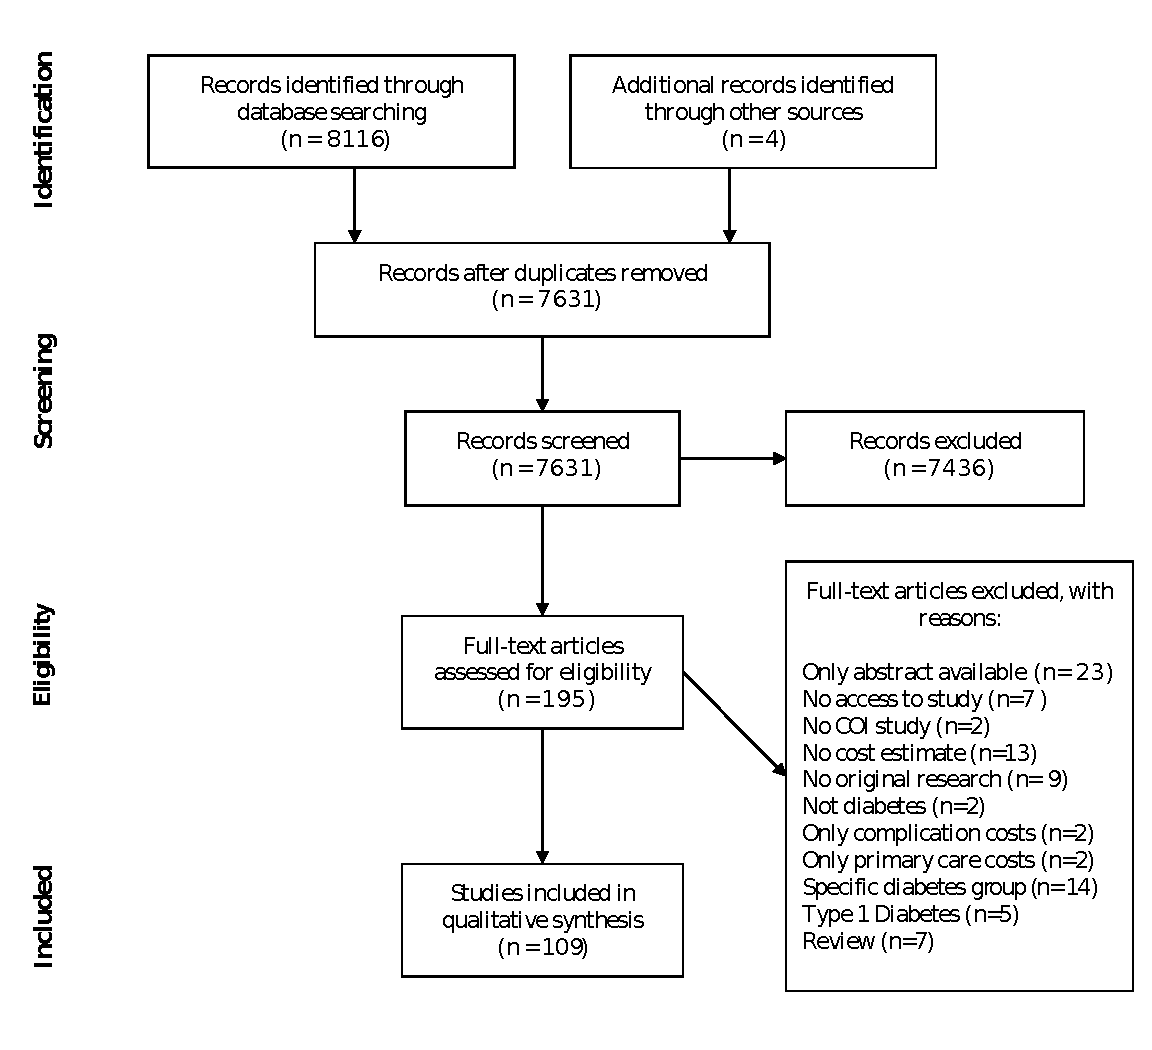
\includegraphics[width=0.9\linewidth]{Review/Figures/Fig1.eps}
\end{figure}

We present the \ac{COI} study results in per capita values to facilitate comparability across countries. For studies presenting overall population level estimates rather than per capita costs information, we calculated those costs, whenever possible, using the diabetes prevalence mentioned in the respective study. If no total cost estimate was presented but information on direct and indirect costs was available, then direct and indirect costs were added up to produce a total cost estimate. We converted costs into \ac{PPP} adjusted estimates, also called international dollars and henceforth denoted with the \$ sign, in order to further increase comparability. Since some studies did not present the data in the country's local currency but in USA\$ or some other major currency, we used the exchange rate given in the article to convert the estimates back into the local currency. If no exchange rate was provided in the study itself, the average exchange rate (midpoint exchange rate according to OANDA historical exchange rates---[\url{http://www.oanda.com/currency/historical-rates/}]) for the reported year. The \ac{PPP} adjusted estimates for the year 2011 were then calculated using the Campbell and Cochrane Economics Methods Group Evidence for Policy and Practice Information and Coordination Centre (CCEMG-EEPPI Centre) cost converter \parencite{Shemilt2010}. For all additional analyses carried out in the following sections only studies for which a mean cost estimate was presented or could be calculated, were included. Further, in the case of a study presenting estimates for more than 1 year, only the estimate for the most recent year was used for the analysis. For studies presenting both incremental and total cost estimates, only the incremental cost estimate was taken into account.

Studies were further classified into two groups according to the level of economic development of the investigated country---(1) high-income and (2) \acp{LMIC} (\acp{LMIC})---according to the historical World Bank income group classification of the respective country in the year that data collection for the respective study had taken place \parencite{WorldBank}. Where necessary due to space constraints we used abbreviations for country names, as detailed in Table \ref{tab:review_countries} in the appendix.

In order to explore the factors involved in the variation of direct costs reported in \ac{COI} studies, we first plotted the direct per capita costs in relation to the \ac{GDP} per capita of the respective country and provided an estimate of the relationship using linear regression. We then conducted an exploratory regression analysis, with the annual direct cost per patient as the dependent variable to investigate what other factors might explain the variation in direct cost estimates. The set of independent variables comprised (1) the estimation approach in each study, (2) the year of data used, (3) \ac{GDP} per capita of the studied country in international dollars, (4) an indicator of whether the study was conducted in the USA, (5) an indicator of whether the study was deemed to be nationally representative, and (6) a variable indicating whether the study had explicitly taken diabetes-related complications into account. The year of the data used was considered because the development of social security systems and treatment methods may affect how the direct costs evolve over time. We categorized this variable into groups: studies using data from before 1995, 1995 to 1999, 2000 to 2004, 2005--2009 and 2010--2004.  The dummy variable for studies on the USA was included to account for the generally higher healthcare expenditures in the USA compared which other \acp{HIC} with similar per capita income levels \parencite{Laugesen2011}. Accounting for national representativeness should cancel out any effects that might be driven by those studies that estimate costs for sub-national, regional- or city-level population samples. Including an estimator for diabetes complications should account for the possible underestimation of diabetes costs in studies excluding complications. We exclude country estimates extracted from multi-country studies in our preferred specification, as their inclusion would lead to an over-statement of the cost effect of the estimation method employed in the given multi-country study. 

\section{Results}
Due to the differences in methodologies, we first present the findings on the identified \ac{COI} studies and subsequently turn to studies on labour market outcomes.

\subsection{Cost-of-illness studies on type 2 diabetes}

\subsubsection{Number of studies}
We identified a total of 86 relevant \ac{COI} studies (see Table \ref{tab:COI_charactersitics} in the appendix for a detailed description of the included studies), of which 62 focused on \acp{HIC}, 23 on \acp{LMIC}, and one multi-country study covered both \acp{HIC} and \acp{LMIC}. Studies in \acp{LMIC} increased over time, with the majority of the \ac{LMIC} studies being published between 2007 and 2014. Six of the selected studies were multi-country studies, of which two \parencite{Kirigia2009,Smith-Spangler2012} did not provide detailed cost estimates for every country in the study and one did not provide a year for the estimated costs, so that we could not calculate estimates in international dollars \parencite{Boutayeb2014}. Therefore, we could not include these particular studies in our country-specific analysis.

\subsubsection{Regional distribution}
In terms of geographic regions, most studies were carried out on countries in Latin America and the Caribbean (n=38) and Europe (n=37), followed by the USA and Canada (n=26), East Asia and Pacific (n=11), the Middle East and North Africa (n=5), South Asia (n=4), Sub-Saharan Africa (n=4) and Australia (n=1). The number of countries studied is higher than the number of articles reviewed due to four multi-country studies \parencite{Boutayeb2014,Barcelo2003,Jonsson2002b,Abdulkadri2009b}, estimating costs for multiple countries. The USA were the most studied country (n=19), followed by Canada (n=7) and Germany (n=5). Mexico (n=6) and China (n=4) were the most frequently studied \acp{LMIC}.

\subsubsection{Data sources}
Especially in \acp{LMIC}, self-administered surveys represented a popular method to retrieve data on the cost of diabetes. These were mostly limited regionally, i.e. to a city or hospital, and usually only representative of these regional diabetes populations but not of a national population. In \acp{HIC}, databases of insurance and healthcare providers were the main source of information in most studies. These data tended to be representative either at a national or at some sub-national level. As a result, the size of the samples in \acp{HIC} was mostly between 1,000 and several million. By contrast, studies in low- and lower-middle-income countries were generally characterized by smaller sample sizes, ranging from 35 \parencite{Suleiman2006} to about 2,433 \parencite{Yang2012} in the studies reviewed here.

\subsubsection{Variation in costing approaches}
As discussed in more detail in Text Box 1, a range of costing approaches can be found in the \ac{COI} literature. Figure \ref{fig:review_COI_number} shows that the most common costing method for the direct costs of diabetes in \acp{HIC} was the sum-all medical approach for people with diabetes without using control groups \parencite{Kirigia2009,Boutayeb2014,Barcelo2003,Jonsson2002b,Ohinmaa2004,Lau2011a,Pohar2007,Gonzalez2009b,Horak2009,Martin2007b,Nolan2006c,Lucioni2003,Morsanutto2006b,Nakamura2008,Arredondo2004,Arredondo2007,Arredondo2005a,Arredondo2011b,Redekop2002b,Bjegovic2007b,Oliva2004a,Ringborg2008a,Chi2011a,Zhou2005a,Condliffe2014,Brandle2003d,Peele2002a,Lee2006,Maciejewski2004}. 

The disease-attributable costing approach \parencite{Suleiman2006,Abdulkadri2009b,Davis2006b,Simpson2003,RodriguezBolanos2010a,Solli2010a,Ballesta2006,Mata2002a,Lin2004,Dall2003a,Buescher2010,Tunceli2010c,Johnson2006d,Honkasalo2014,Bastida2002} and the attributable-fraction approach were also used widely, though mainly in the USA \parencite{AmericalDiabetesAssociation2008,Dawson2002b,Schmitt-Koopmann2004b,Dall2010,Bolin2009d,Honeycutt2009a,Lesniowska2014}. 

The incremental cost approach was applied primarily in studies on \acp{HIC} \parencite{Smith-Spangler2012,Yang2012,Tunceli2010c,Honeycutt2009a,Pohar2007a,Ricordeau2003,Koster2011c,Koster2006c,Koster2012,Esteghamati2009,Chodick2005a,Marchesini2011b,Bruno2012,Norlund2001a,Wirehn2008b,Birnbaum2003c,Durden2009b,Rodbard2010b,Oconnell2012,Trogdon2008a,Ramsey2002a,VanderLinden2009c}.  

For \acp{LMIC}, the survey approach was the most used \parencite{Wang2009b,Wang2009f,Chan2007a,Ramachandran2007d,Javanbakht2011b,Khowaja2007a,Biorac2009a,Elrayah-Eliadarous2010b,Chatterjee2011c,Al-Maskari2010c,Druss2001,Tharkar2010a,Wang2010c}.


\begin{figure}[p]
\caption{\label{fig:review_COI_number}Number of \acs*{COI} studies, by costing approach and income group.}%

\begin{minipage}{\linewidth}
\begin{center}
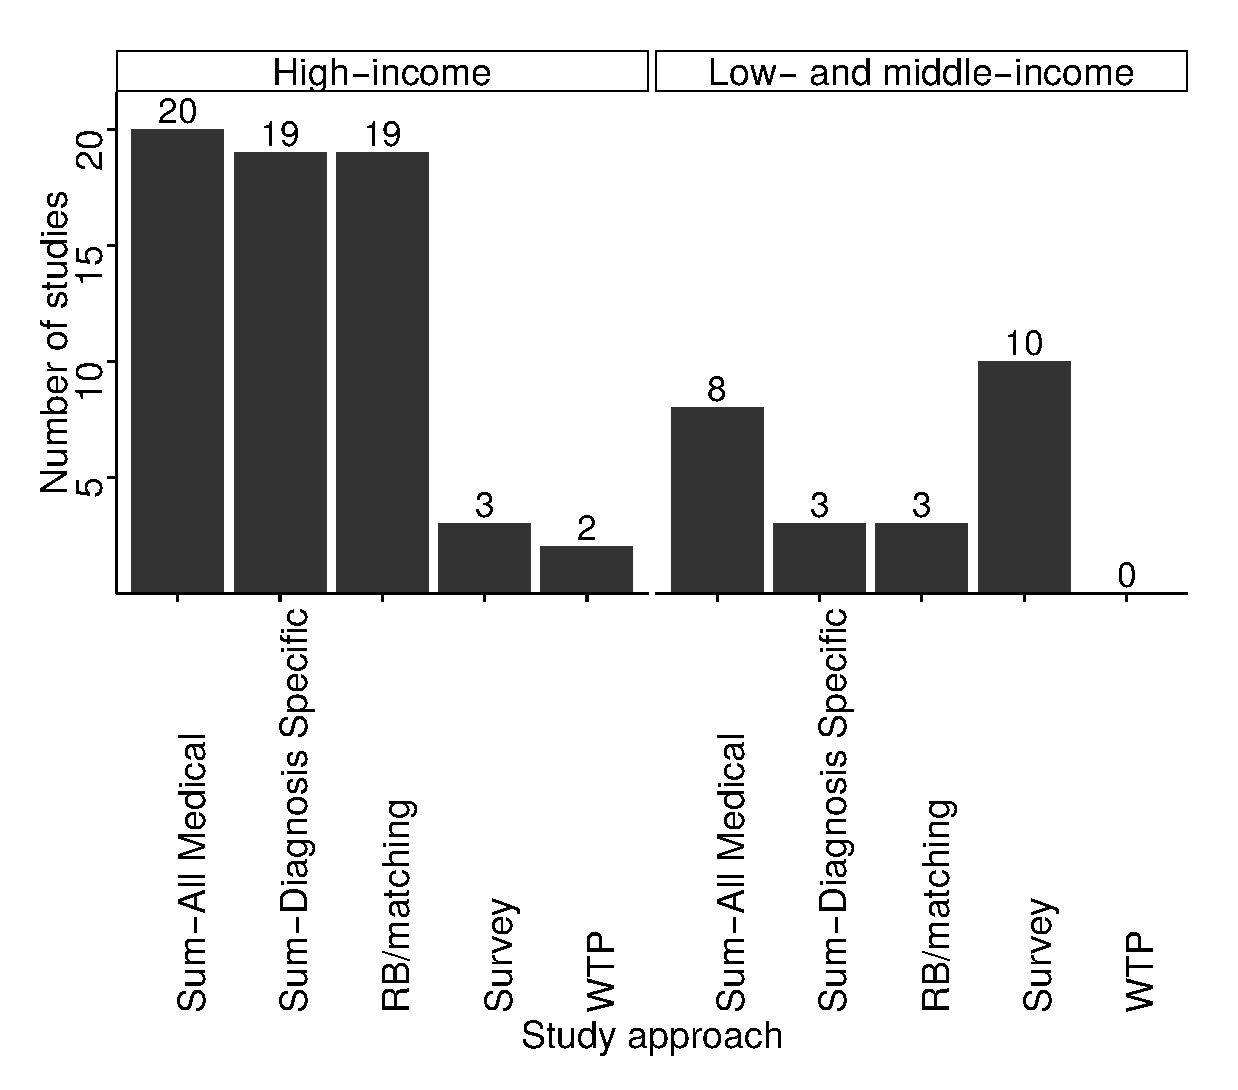
\includegraphics[width=0.8\linewidth]{Review/Figures/Fig2.eps}\\
\end{center}
\footnotesize \textit{Notes} For \acp{LMIC} no \ac{WTP} study is counted, because the only study \parencite{Tharkar2010a} presenting a \ac{WTP} estimate for a \ac{LMIC} used primarily a different approach to estimate costs, and the \ac{WTP} estimate was only presented additionally. Therefore this study was not counted under \ac{WTP} here. Two studies are counted twice as they give estimates for a sum-diagnosis specific and a RB/matching approach.
\end{minipage}
\end{figure}

By contrast, almost all indirect cost assessments followed the same methodology, i.e. the human capital approach. This approach considers all forgone labour earnings of a patient or caregiver that are attributable to diabetes. A minority of three studies \parencite{Tharkar2010a,Chang2010b,Gyldmark2001}, estimated the indirect costs using the \ac{WTP} approach, which tries to measure how much individuals would be willing to pay to reduce the risk of an illness \parencite{Segel2006}, here diabetes (or certain complications associated with it). One of the studies included \ac{WTP} estimates in addition to the direct and indirect costs measured by the human capital approach \parencite{Tharkar2010a} but did not include the \ac{WTP} estimate in the overall cost estimate, while the other two studies estimated exclusively the \ac{WTP} \parencite{Chang2010b,Gyldmark2001}.


\subsubsection{Study perspective}
Studies also varied in their perspective, again compromising direct comparability of the cost estimates across studies. Overall, most studies either took a societal (n=32) or healthcare system perspective (n=48). The former generally takes into account the direct and indirect monetary costs that arise to society, including costs to the healthcare system, costs due to lost productivity and sometimes \ac{OOP} costs \parencite{Segel2006}. The latter was especially common in \acp{HIC} where many studies assessed the cost of diabetes to private or public health insurances. In \acp{LMIC}, studies often took the patient perspective (n=5), estimating \ac{OOP} expenditures and in some cases productivity losses, directly arising to the diabetes patient.

%Textbox
\fbox{\parbox[c]{\linewidth}{\textbf{Text box 1 \ac{COI} methodologies}
\begin{footnotesize}

Methodologies for \ac{COI} studies can broadly be categorized into two main categories:(1) estimating the total disease costs and (2) estimating the incremental costs \parencite{Akobundu2006}. Studies can then be divided further according to the specific approach used for estimation. Our categorization builds on that by \textcite{Akobundu2006} in their review of \ac{COI} methodologies.

\begin{enumerate}

\item Total disease costs
\begin{enumerate}
\item Sum-All Medical: captures all medical expenditures of a person diagnosed with diabetes, irrespective of the relation of the expenditures with diabetes.

\item Sum-Diagnosis Specific: includes the costs that are related to diabetes. This can be done by using a disease-attributable costing approach, using administrative claims databases to identify the cost of diabetes by respective \ac{ICD} codes that link the expenditures to a primary or secondary diagnosis of diabetes as the reason for the healthcare utilization. Alternatively, a similar technique used at the population level is the attributable-fraction approach, where the relative contribution of, e.g., diabetes, to the risk of developing another disease (e.g. renopathy or cardiovascular disease) is used to determine how much of the costs of this disease can be attributed to diabetes.

\item Survey approach: while not specifically mentioned by \textcite{Akobundu2006}, for this review we create a separate category capturing studies using surveys of people with diabetes. This category differs from the two approaches a) and b) above in that estimations rely solely on the individual, reported experience of people with diabetes, without use of any diagnostic data at an aggregate level. The survey approach was also used as a separate category in the earlier review on diabetes \ac{COI} studies by \textcite{Ettaro2004}.
\end{enumerate}

\item Incremental disease costs

There are two main approaches for the estimation of incremental medical costs:
\begin{enumerate}

\item Regression approach: a statistical technique which can account for observable differences between the group with diabetes and the control group (i.e. those without diabetes) to find---ideally---the independent effect of diabetes on healthcare costs. The differences typically accounted for are age, region and gender.

\item Matching approach: uses a control group to directly compare those with diabetes to those without diabetes after matching each person of the 'treatment' group to a 'similar' person of the control group, using various categories like age, region and gender to---again---find the independent effect of diabetes on healthcare cost \parencite{Akobundu2006}.
\end{enumerate}
\end{enumerate}

All of the above approaches can be used in prevalence or an incidence based study. In the former case the costs of diabetes are estimated for a certain point in time, typically one year, while the latter approach estimates costs over a person's lifetime or several years, always starting with the point at which the disease is diagnosed. Both approaches may also be combined in studies estimating the future cost burden of type 2 diabetes by first taking a prevalence approach to calculate current costs and then using predictions about future diabetes incidence rates to arrive at an estimate of diabetes costs at a certain point in the future.\end{footnotesize}
}}

\subsubsection{Costing components}
Of the 75 studies that reported the cost components they used to estimate direct costs, 72 took into account outpatient hospital visits, 70 inpatient hospital visits, 63 physician visits, 58 drug costs, 51 laboratory costs for diagnostic tests and check-ups, 37 equipment costs and 21 non-medical and transportation costs. A total of 46 studies had at least included the costs of hospital, outpatient and physician visits as well as drugs (see Table \ref{tab:costing_components} for a detailed description of cost components used in each study).

\subsubsection{Cost estimates of diabetes using a prevalence approach}

Two basic epidemiological approaches exist for the estimation of \ac{COI}, and they  are not directly comparable. The incidence approach follows people with diabetes, usually starting with their diagnosis at a common base year, estimating yearly costs for a sample of people at the same disease stage, finally giving an estimate of diabetes costs over a certain time period, such as from diagnosis to death or over a distinct period of, for example, 10 years. This approach can also document how costs of diabetes change and develop over the progression of the disease \parencite{Larg2011}. By contrast, the prevalence approach estimates the costs of diabetes for a cross-section of people with diabetes at a certain point in time, normally a year, who are at different stages of the disease. It is most suitable for assessing the total economic burden of diabetes at a certain point in time. Due to this difference in time periods and the data used, the estimates of prevalence-based studies are not directly comparable with those of incidence-based studies. Hence, we present the cost estimates, starting with the prevalence approach.

Table \ref{tab:review_regression} shows the range of direct cost estimates by estimation approach and income status.  As can be observed, direct cost estimates varied widely, both between and within the different estimation approaches. Cost estimates for direct costs, irrespective of the costing method applied and the cost components included, ranged from \$242 for Mexico \DIFdelbegin %DIFDELCMD < \parencite{,Arredondo2005a} %%%
\DIFdelend \DIFaddbegin \parencite{Arredondo2005a} \DIFaddend in 2010 to \$11,917 for the USA \parencite{Condliffe2014} in 2007. Also, studies from \acp{LMIC} generally indicated smaller direct costs than studies from \acp{HIC}.

For indirect costs, studies using the human capital approach estimated costs ranging from \$45 for Pakistan \parencite{Khowaja2007a} in 2006 to \$16,914 for the Bahamas \parencite{Barcelo2003} in 2000. Three studies estimated indirect costs by using the \ac{WTP} approach and found costs ranging from \$191 in a study on the \ac{WTP} for a health insurance for type 2 diabetes in Denmark in 1993 \parencite{Gyldmark2001}, a \ac{WTP} \$4,004 per year for a cure of type 2 diabetes \parencite{Chang2010b} in Taiwan  and an annual payment of \$4,737 to halt disease progression/prevent future complications of diabetes in India \parencite{Tharkar2010a}. 

Societal costs of type 2 diabetes, which are estimated by studies combining direct and indirect costs, ranged from \$544 in a study on the economic costs of diabetes in Iran \parencite{Esteghamati2009} in 2001 to \$18,224 for the Bahamas \parencite{Barcelo2003} in 2000. 

\begin{table}[p]
\begin{center}

\begin{threeparttable}
\begin{tabularx}{\linewidth}{X X X X X X X X X}
\caption{\label{tab:review_direct_costs_summary}Summary of direct costs by estimation approach and income status in international dollars \$ (2011) for prevalence-based studies.}\\
\toprule
& \multicolumn{4}{l}{High-income countries} & \multicolumn{4}{l}{Low- and middle-income countries} \\ \midrule
 & Sum-all medical costs & Sum-diagnosis specific & RB / matching & own survey & Sum-all medical costs & Sum-diagnosis specific & RB / matching & own survey \\ \midrule \endfirsthead
\caption[]{Summary of direct costs by estimation approach and income status in international dollars \$ (2011) for prevalence-based studies.}\\
 \toprule
 & \multicolumn{4}{l}{High-income countries} & \multicolumn{4}{l}{Low- and middle-income countries} \\ \midrule
  & Sum-all medical costs & Sum-diagnosis specific & RB / matching & own survey & Sum-all medical costs & Sum-diagnosis specific & RB / matching & own survey \\ \midrule \endhead
Min & 1117 & 907 & 264 & 1495 & 242 & 662 & 443 & 456 \\
Max & 11917 & 9346 & 8306 & 5585 & 4129 & 4672 & 1136 & 3401 \\
N & 25\textsuperscript{a} & 19\textsuperscript{a} & 18 & 3 & 27\textsuperscript{a} & 5\textsuperscript{a} & 2 & 10\\
 \bottomrule
\end{tabularx}
\begin{tablenotes}
\item \footnotesize \textit{Notes} \textsuperscript{a} Includes country estimates from multi-country studies; RB Regression based
\end{tablenotes}
\end{threeparttable}
\end{center}
\end{table}


In order to improve the cross-country comparability of the costs of diabetes we plotted the results from studies providing a direct per capita cost estimate against the \ac{GDP} per capita estimate of the respective country (we limited this comparison to studies using samples representative of their entire population). Figure \ref{fig:review_GDPtocost_ratio} confirms the expectation that costs do increase with economic wealth: \ac{GDP} per capita explains about one-third of the variation in cost estimates (see r2 in Figure \ref{fig:review_GDPtocost_ratio}). Also, studies on the USA seem to estimate costs consistently higher than would be expected on the basis of its \ac{GDP} per capita. 

The USA, however, spend consistently more than what would be expected on the basis of its \ac{GDP} per capita. Again, the wide variation in estimated costs for many countries underscores the point that the studies need to be contextualized and may not be directly comparable per se. On the whole---though by no means always---the matching and regression as well as the sum-diagnosis specific approaches appear to produce lower cost estimates than especially the total cost results, particularly so for \acp{HIC}. In an inevitably crude attempt to quantitatively explore the driving factors behind the heterogeneity in cost estimates, we estimated a simple linear regression model with per capita direct costs as the dependent variable; explanatory variables included \ac{GDP} per capita, the estimation approach employed by the study, the number of included cost components, a dummy for studies carried out in the USA, the year of data collection, the representativeness of the study and if the study included diabetes complications as explanatory variables. The results, displayed in Table \ref{tab:review_regression}, show a strong relationship between \ac{GDP} per capita and expenditures for diabetes, with every additional international dollar in per capita \ac{GDP} translating into an average increase in direct diabetes expenditures of about \$0.04. The estimation approach is not found to matter significantly, nor is the year of study. Estimates from USA studies put the costs at over \$3,000 higher (on average) than studies from other countries, indicating that costs in the USA may indeed be unusually high. The number of costing components and the inclusion of complications likely also explain some of the variance in estimates, although they are just below and above the 10\% significance level, respectively. Overall, the included independent variables explain about 56\% of the variation in direct cost estimates. In a sensitivity analysis, we included the results from multi-country
studies providing country estimates in the regression analysis. The
only major difference to the presented analysis is that the inclusion of
complications as well as the number of included cost components
were now significant at the 1\% and 5\% significance level, respectively.
The effect size and significance of the other estimates did not change
considerably.


\begin{figure}[p]
\caption{\label{fig:review_GDPtocost_ratio}\acs*{GDP} to direct costs ratio by estimation approach.}%
\begin{minipage}{\linewidth}
\begin{center}
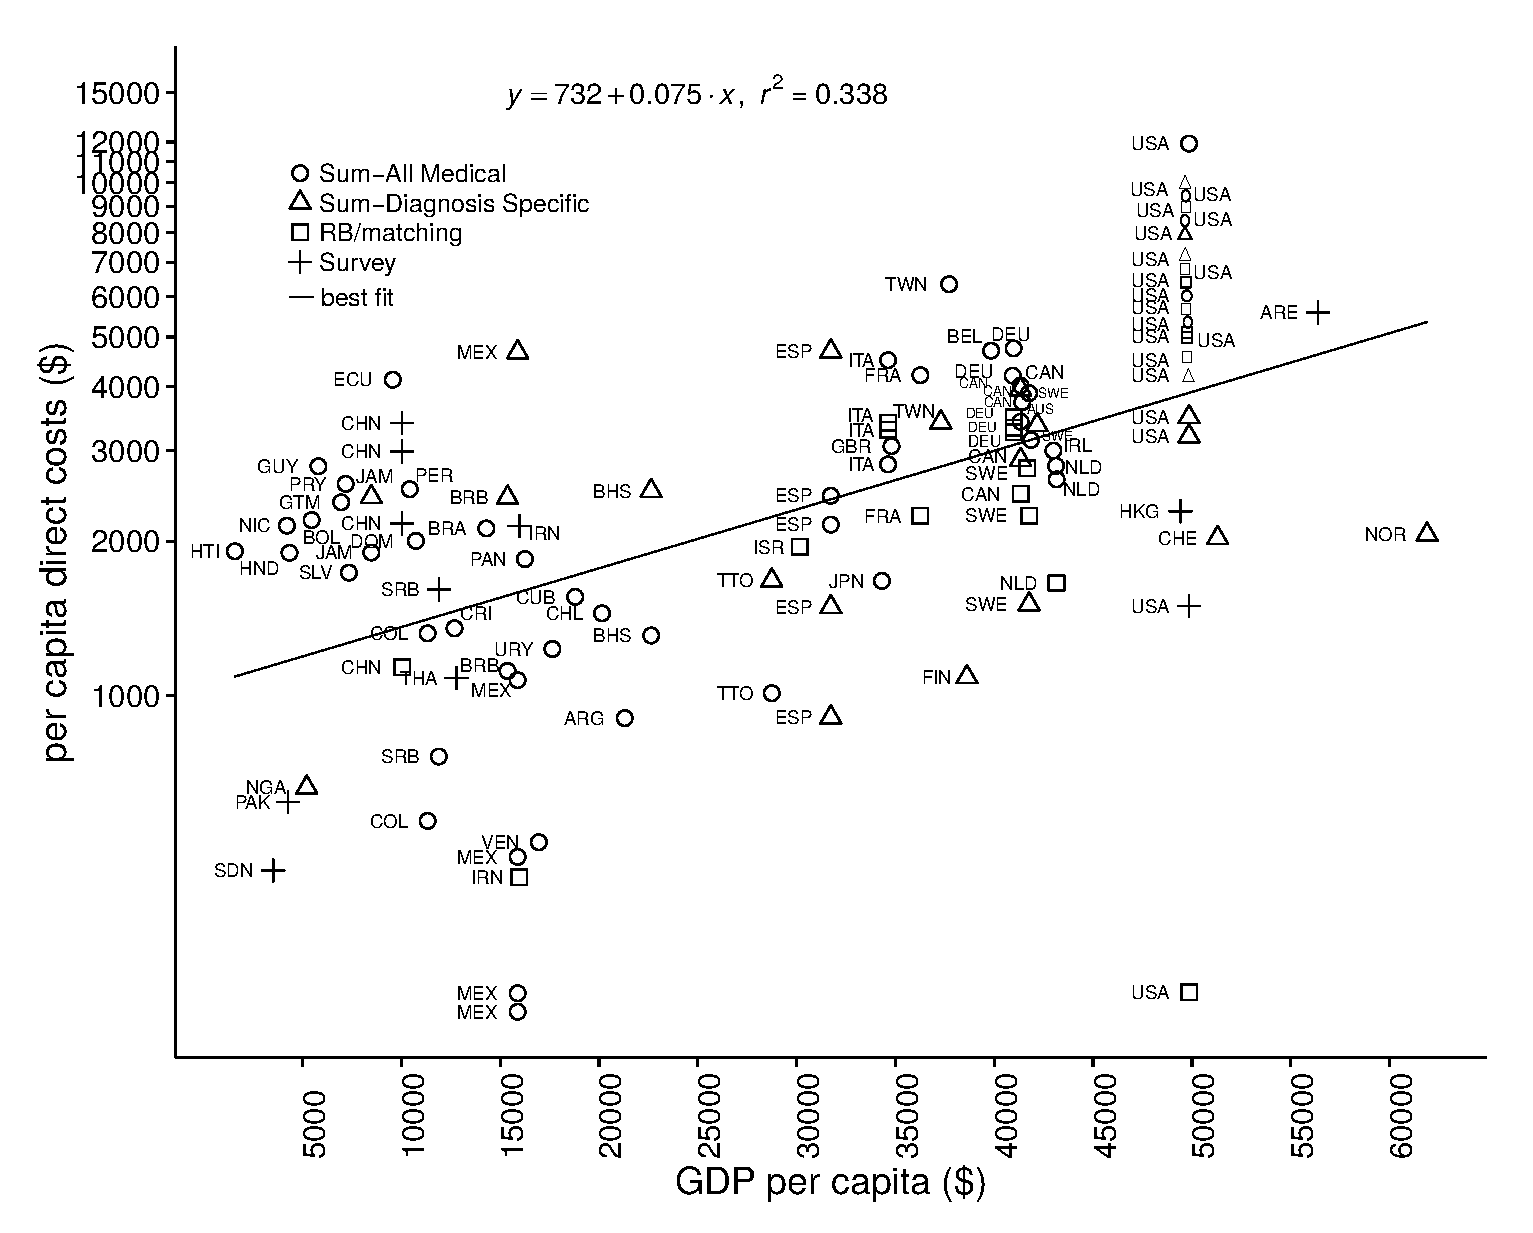
\includegraphics[width=1\linewidth]{Review/Figures/Fig3.eps}\\
\end{center}
\footnotesize
\textit{Notes}  The line depicts the best fit based on the linear regression of direct costs on \ac{GDP} per capita in international dollars.
\end{minipage}
\end{figure}





\begin{table}[p]
\caption{\label{tab:review_regression}Relationship between direct costs and study characteristics (robust linear regression).}
\begin{center}
\begin{adjustbox}{max width=\linewidth}
\begin{threeparttable}
{
\def\sym#1{\ifmmode^{#1}\else\(^{#1}\)\fi}
\begin{tabular}{l*{2}{SS}}
\toprule
                 &\multicolumn{1}{c}{Estimate} &\multicolumn{1}{c}{Std. Error} \\ \midrule
                Constant & 2133 & 1773.922 \\
                GDP per capita (\$) & .045\sym{**} & 0.017 \\
                Estimation Approach &  &  \\
                \hspace*{10mm}Sum-All medical (Ref.) & &  \\
                \hspace*{10mm}Sum-Diagnosis Specific & -413.880 &  528.766 \\
                \hspace*{10mm}RB/matching & -719.868 &  526.896 \\
                \hspace*{10mm}Survey & -689.806 & 671.020 \\
                At least four costing components & 702.966\sym{*} & 403.968 \\
                USA study & 3111.067\sym{***} & 533.534 \\
                Year of study &  &  \\
                \hspace*{10mm}\textless1995 (Ref.) &  &  \\
                \hspace*{10mm}1995-1999 & -1744.799 & 1632.498 \\
                \hspace*{10mm}2000-2004 & -816.647 & 1586.966 \\
                \hspace*{10mm}2005-2009 & -1021.685 & 1592.595 \\
                \hspace*{10mm}2010-2014 & -2744.739 & 1839.689 \\
                Study representative & -598.670 & 409.070 \\
                Complications & 666.803 & 414.727 \\
\midrule
                R-squared adj. & .559 &  \\
                N & 70 &  \\ 
 \bottomrule
\end{tabular}
\begin{tablenotes}
\item \footnotesize \textit{Notes} Standard errors in parenthesis. Ref. reference category.
\sym{*} \(p<0.10\), \sym{**} \(p<0.05\), \sym{***} \(p<0.01\).
\end{tablenotes}
}
\end{threeparttable}
\end{adjustbox}
\end{center}
\end{table}

The sensitivity of the cost results to the estimation approach was also examined by two studies that investigated the effect of different estimation techniques in diabetes \ac{COI} studies. \textcite{Honeycutt2009a} compared the use of a regression-based and an attributable-fraction approach and found that the cost estimate of the former exceeded the latter by 43\%. \textcite{Tunceli2010c} compared the matching and the diabetes (disease)-attributable costs approach and found a 14--29\% higher cost estimate using matching, depending on the assumptions used. Both studies concluded that an incremental cost approach results in a higher, and likely more exact, estimate of the direct costs of diabetes than disease-attributable approaches. The authors attributed this to the fact that a regression or matching approach can assign costs to diabetes that cannot be linked to diabetes otherwise. Those approaches are therefore in a position to account for all costs of co-morbidities caused by diabetes, while this is not automatically the case with the other approaches.

\subsubsection{Direct and indirect costs of diabetes}

\DIFdelbegin \DIFdel{To assess }\DIFdelend \DIFaddbegin \DIFadd{Comparing }\DIFaddend the relative importance of direct and indirect costs across countries \DIFdelbegin \DIFdel{, we }\DIFdelend \DIFaddbegin \DIFadd{may provide some information regarding the underlying drivers of costs due to diabetes in different countries. For instance, a higher ratio of direct to indirect costs may indicate that the higher direct expenditures have lead to better treatment and less complications and thereby have reduced the productivity losses due to diabetes. We therefore }\DIFaddend plotted direct against indirect costs from studies that provided both estimates and drew a 45\degree line depicting the equal share of direct and indirect costs (see Figure \ref{fig:review_direct_indirect}). \DIFaddbegin \DIFadd{Studies above the line found higher direct costs compared to indirect costs and studies below the line found higher indirect costs compared to direct costs.
}\DIFaddend 

Most studies found a larger share for direct costs in comparison with indirect costs\DIFdelbegin \DIFdel{(observations above the 45}%DIFDELCMD < \degree  %%%
\DIFdel{line in Figure \ref{fig:review_direct_indirect})}\DIFdelend . This is especially true for \acp{HIC}, where only a study on Sweden \parencite{Bolin2009d} found a larger share for indirect costs. For \acp{LMIC}, a study on Colombia \parencite{Gonzalez2009b} found considerably higher indirect costs, as did the multi-country study of \textcite{Barcelo2003} and a study on various countries in the African region \parencite{Kirigia2009}, which both found higher indirect costs for almost every country in the study and also on average for the entire \DIFdelbegin \DIFdel{regions}\DIFdelend \DIFaddbegin \DIFadd{region}\DIFaddend , represented as the mean overall study estimate in Figure \ref{fig:review_direct_indirect}.  Both studies used similar approaches to estimate costs, and indirect cost estimates were likely so high because evidence from only a few countries within the region was used as a basis for estimating indirect costs for every other country in the respective study. Further, the studies took the countries' per capita gross national product as a proxy for earnings, which might have led to an over-estimation of the indirect costs \parencite{Kirigia2009}. 

\DIFaddbegin \DIFadd{Overall, no clear pattern emerges that would indicate that in }\acp{LMIC} \DIFadd{indirect costs would be higher than direct costs due to their less extensive healthcare systems, or that }\acp{HIC} \DIFadd{would be able to prevent indirect costs as a result of their higher healthcare spending. For instance, while some studies indicated that }\acp{MIC} \DIFadd{such as Colombia and Mexico have higher indirect costs, studies on China, Pakistan and, again, Mexico showed the opposite. Difficulties in measuring costs could be one of the main reasons for the heterogeneity in results even for the same country and may make a comparison of direct and indirect costs difficult. In particular in }\acp{LMIC} \DIFadd{countries, direct healthcare expenditures may be low due to limited availability and access to healthcare so that direct costs would be higher if more treatment options were available. Indirect costs may also be incorrectly measured, for example the use of the human capital approach---which assumes that productivity losses due to a disease are permanent, even though in reality production losses may only be temporary until the employer has found a replacement---may lead to an overestimation of the losses in productivity }\parencite{Segel2006}\DIFadd{. 
}

\DIFaddend \begin{figure}[p]
\caption{\label{fig:review_direct_indirect}Direct and indirect cost relation in studies estimating total costs of type 2 diabetes.}%
\begin{minipage}{\linewidth}
\begin{center}
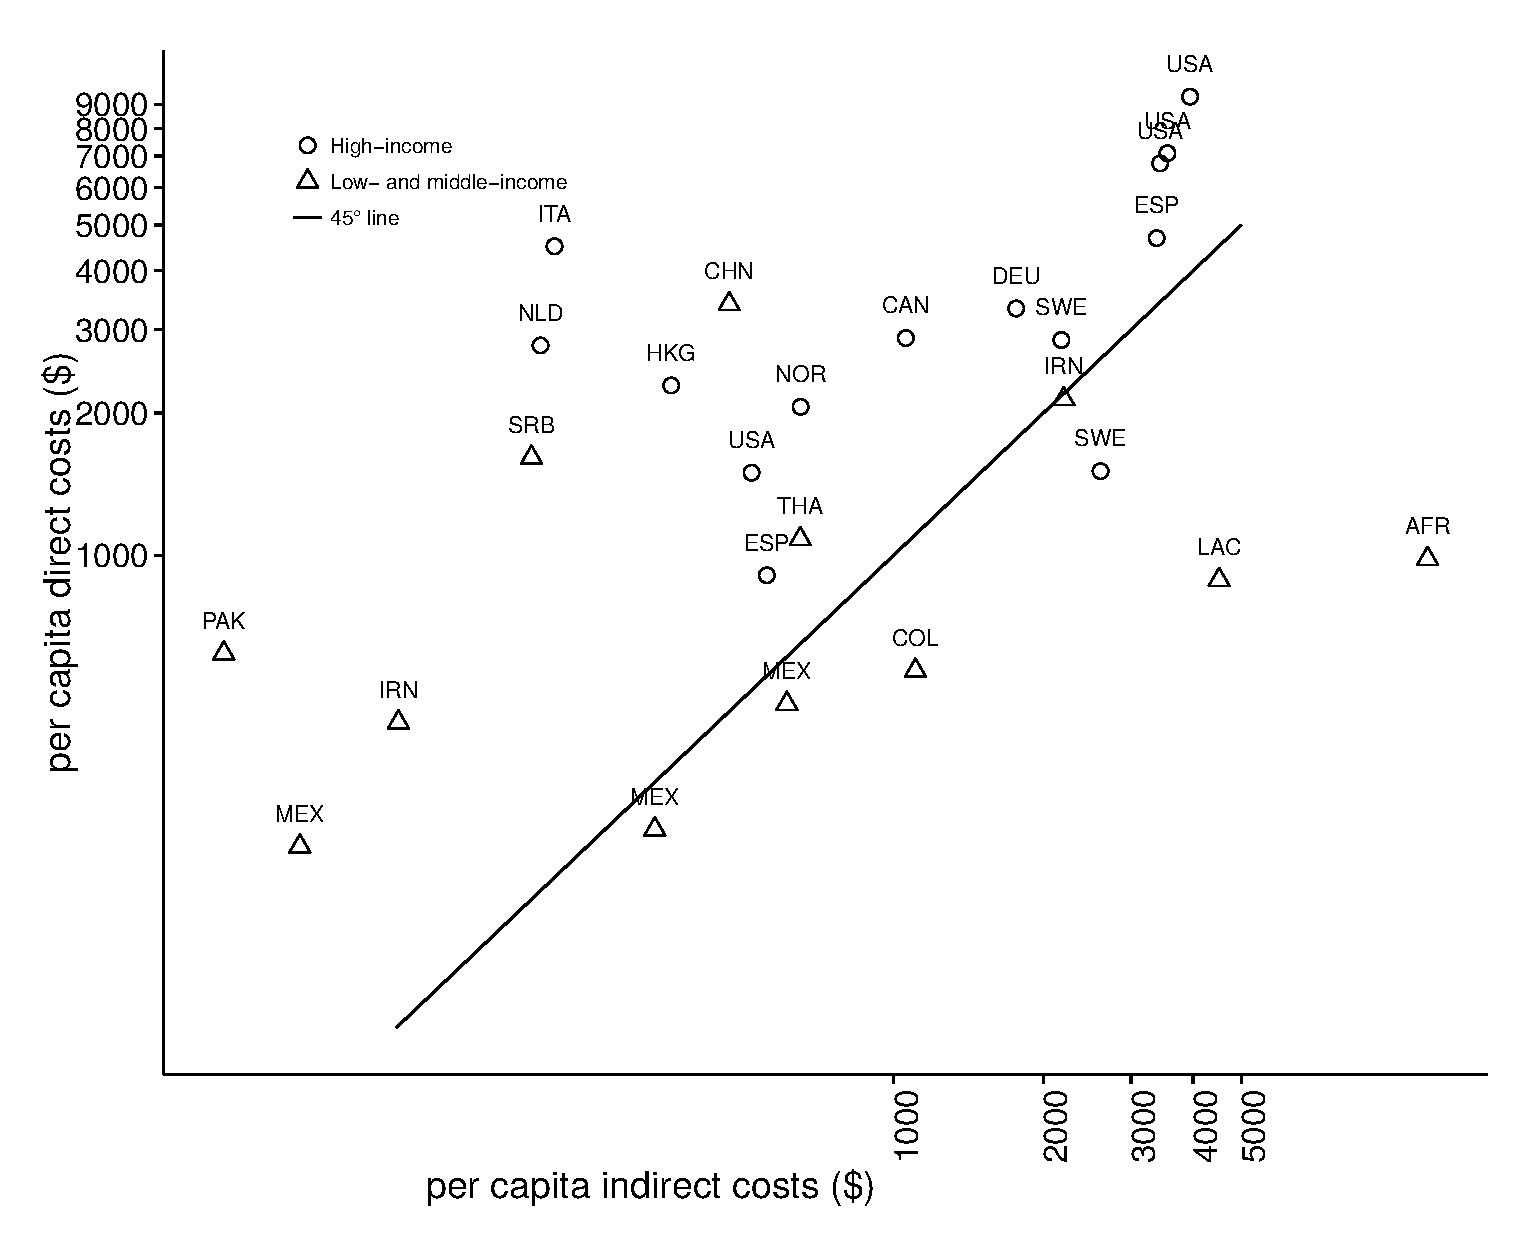
\includegraphics[width=1\linewidth]{Review/Figures/Fig4.eps}\\
\end{center}
\footnotesize
\textit{Notes} The 45\degree line depicts the points where direct and indirect costs would be equal. Above the line direct costs are higher than indirect costs and vice versa. For better visibility both coordinate axes are expressed in log scale
\end{minipage}
\end{figure}

\subsubsection{Studies using the incidence approach}
The four studies that used an incidence approach (see Table \ref{tab:review_incidence}) estimated the cost of diabetes either over a person's lifetime \parencite{Gonzalez2009b,Birnbaum2003c} or over a certain period after diagnosis \textcite{Johnson2006d,Martin2007b}. \textcite{Gonzalez2009b} modelled the lifetime (direct and indirect) costs of a typical diabetes patient in Colombia, arriving at a mean cost estimate of \$54,000. The second study providing lifetime estimates by \textcite{Birnbaum2003c}, estimated incremental lifetime healthcare costs for USA females with diabetes of \$283,000.

Two studies followed patients over a limited time period and found different patterns in the development of type 2 diabetes-attributable healthcare costs. In Germany costs increased from  \$1634 in the first year after diagnosis to \$4881 in the seventh year \parencite{Martin2007b}. In Canada, \textcite{Johnson2006d} found the highest costs in the year of diagnosis with \$7635, up from \$2755 the year prior to diagnosis. In the year after diagnosis costs decreased to \$4273 and then only increased slightly to \$4618 in year ten. In Germany and Canada, costs related to complications or hospital visits were the most important components and in Germany increased steadily over time. In Canada costs related to prescriptions increased the most.

\clearpage
\begin{landscape}

\begin{tabularx}{\linewidth}{m m m b m b}
\caption{Incidence studies on the costs of diabetes}\label{tab:review_incidence}\\
\toprule
Ref. &  Country & Time horizon & Population & Approach & \multicolumn{1}{c}{Results} \\
 \midrule \endfirsthead
\caption[]{Incidence studies on the costs of diabetes}\\
\toprule
Ref. &  Country & Time horizon & Population & Approach & \multicolumn{1}{c}{Results} \\ \midrule \endhead
\textcite{Johnson2006d} &  Canada & 1992--2001 & Incidence T2D patients from Saskatchewan Health's administrative database in Canada & Sum-all medical & Highest  total healthcare costs at year of diagnosis with CAN\$7343 (\$7635), then increased from a low of CAN\$3880 (\$4034) 3 years after diagnosis to CAN\$4441   10 years thereafter (\$4618). \\
	\textcite{Gonzalez2009b} & Colombia & 32 years & Hypothetical average Columbian T2D patient & Sum-all medical & Total lifetime costs (32 year  period) of average diabetes patient, including direct and indirect costs,  57.565 million Colombian pesos (\$54,351). \\
\textcite{Martin2007b} & Germany & 1995--2003 & Newly  diagnosed T2D patients from randomly drawn practices across Germany & Sum-all medical & EUR 1,288   (\$1635) for the first treatment year after diabetes diagnosis and increased   to EUR 3845 (\$4880) in the seventh year. \\
\textcite{Birnbaum2003c} & United  States & 1997--1998 & Women employed by nationwide operating company and hypothetical women above age 64 receiving Medicare & RB / matching & \$282973 incremental lifetime direct healthcare costs, using incidence-based, steady-state methodology. \\ \bottomrule
\multicolumn{6}{l}{\footnotesize \textit{T2D} type 2 diabetes}
\end{tabularx}


\end{landscape}



\subsubsection{Country level costs prediction studies}
Four studies projected costs of diabetes over a certain period of time \parencite{Ohinmaa2004,Lau2011a,Davis2006b,Wang2009f}, making assumptions about the future development of diabetes prevalence and population ageing (see Table \ref{tab:review_prediction}). For Canada, a 1.7-fold increase from 2000 to 2016 \parencite{Ohinmaa2004} and a 2.4-fold increase from 2008 to 2035 in diabetes healthcare costs was estimated \parencite{Lau2011a}. Taking a health care system perspective, both studies found that the estimated increase would be mostly driven by an ageing population. For Australia, \textcite{Davis2006b} estimated a 2.5- to 3.4-fold increase in diabetes attributable healthcare costs from 2000 to 2051, depending on the underlying assumptions about population ageing and diabetes prevalence rates. For China, \textcite{Wang2009f} extrapolated total costs of diabetes from the year 2007 to 2030, estimating the costs of diabetes to increase 1.8-fold, solely accounting for the expected increase in prevalence.

\begin{table}[p]
\begin{tabularx}{\linewidth}{m m m m m b}
\caption{Country level costs prediction studies}\label{tab:review_prediction}\\
\toprule
Ref. & Country & Population   & Approach & Time  horizon & \multicolumn{1}{c}{Results}                                                                                                                                            \\ \midrule
\textcite{Davis2006b}  & Australia & Australian   population                       & Sum diagnosis  Specific & 2000--2051                                                              & If age and sex specific prevalence remains unchanged a 2.5-fold increase; if age and sex specific prevalence allowed to change as well a 3.4-fold increase. \\
\textcite{Ohinmaa2004}  & Canada    & Canadian   population                         & Sum-all   medical costs  & 2000--2016                                                              & 1.7-fold increase.                                                                                                                                          \\
\textcite{Lau2011a}  & Canada    & Four   Alberta Health and Wellness databases  & Sum-all  medical costs  & 2008--2035                                                              & 2.4-fold increase.                                                                                                                                          \\
\textcite{Wang2009f}  & China     & In   patients and outpatients in 20 hospitals & Own   survey             & 2007 and  2030 (projection) & Increase from \$73 billion in 2007 to \$132 billion in 2030 (1.8 fold increase).                                       \\ \bottomrule
\end{tabularx}
\end{table}

\subsection{The impact of diabetes on employment probabilities and productivity}
Besides studies that determined the cost of diabetes by costing related expenditures, another body of research has investigated---using econometric techniques---the impact of diabetes on 'productivity', a term used here to comprise outcomes including employment probabilities and lost work days and income or earnings. A recent study systematically reviewed evidence on the impact of diabetes on the ability to work, focusing on studies assessing the impact of diabetes on early retirement, lost work hours, absenteeism and presenteeism \parencite{Breton2013}. We focused particularly on studies exploring the impact of diabetes on employment probabilities and earnings---both issues that were not covered in the mentioned review---and we took a more detailed look at the empirical challenges posed by the issue of endogeneity (see page \pageref{sec:appendix_endogeneity} in the Appendix for a more detailed discussion of endogeneity).

Tables \ref{tab:rev_Diab_employment} and \ref{tab:rev_Diab_productivity} synthesize the relevant information from the 23 identified studies on the effect of diabetes on employment and other labour market outcomes. Almost all studies were conducted on \acp{HIC}, mainly the USA (n=13) and European countries (n=4). Only one study focused on a \ac{LMIC} investigating the effect of diabetes on labour income in China.

\subsubsection{Employment probabilities}
Most studies examined the impact of diabetes on employment probability (n=17), applying a range of econometric techniques. These have evolved over time, and more recent studies took into account the possibility that diabetes might be endogenous: it is conceivable that especially personal traits such as motivation and drive could influence the propensity to develop type 2 diabetes as well as a persons' job market opportunities. Further, being employed or unemployed could also lead to changes in lifestyles, due to changes in income, stress or leisure time, that could themselves affect the chances of developing diabetes \parencite{Brown2005}. Of the studies that tried to account for this problem \parencite{Brown2005,Minor2011,Latif2009,Lin2011b,Zhang2009,Harris2009}, the majority used an \ac{IV} technique. This approach allows for the consistent estimation of the effect of diabetes on employment if a variable can be found that is causally related to diabetes without affecting the employment probabilities through any other unobserved pathway apart from its effect on diabetes (see Text Box 1). In the case of type 2 diabetes all studies used the family history of diabetes as an \ac{IV} to exploit the fact that the development of type 2 diabetes is much more likely for individuals whose biological parents have also had diabetes. It is argued that, while controlling for education, age and other observable demographic and socioeconomic factors (e.g. wealth, regional and ethnic differences and the number of children in the household), having a family member with diabetes should not affect the person's employment status or other labour market outcomes, while strongly predicting the onset of type 2 diabetes. 

\newpage
\begin{landscape}
\begin{tabularx}{\linewidth}{m m m m b b}
\caption{Studies estimating the relationship between diabetes and employment (2001 -- 2014)}\label{tab:rev_Diab_employment}\\
\toprule
Ref & Survey year & Country  & Age     & \multicolumn{2}{c}{Effect on employment} \\ \cmidrule(l){5-6}                                                                                                                                                                                                                                                                                                                                                                              &  &  &   & \multicolumn{1}{c}{Males} & \multicolumn{1}{c}{Females} \\ \midrule \endfirsthead
\caption[]{Studies estimating the relationship between diabetes and employment (2001 -- 2014)}\\
\toprule
Ref & Survey year & Country  & Age     & \multicolumn{2}{c}{Effect on employment} \\ \cmidrule(l){5-6}                                                                                                                                                                                                                                                                                                                                                                              &  &  &   & \multicolumn{1}{c}{Males} & \multicolumn{1}{c}{Females} \\ \midrule \endhead
\textcite{Harris2009} & 1999-2000      & Australia                                                                                 & \textgreater24              & Exogenous: 10.8 percentage points reduction to be in labour force; endogenous: 7.1 percentage points reduction and test indicates endogeneneity.                                                                                                           & Exogenous: 10 percentage points to be in labour force; endogenous: Nine percentage points reduction and test indicates endogeneneity.                                    \\
\textcite{Zhang2009} & 2001, 2004-2005 & Australia                                                                                 & 18-64                       & 50-64: 11.5 percentage points less likely to be in labour force; 18-49: 3.9 percentage points less likely, all effects increase when other chronic diseases are present.                                                                                   & No significant effect for diabetes alone; significant negative effect if other chronic diseases are present.                                                             \\
\textcite{Latif2009} & 1998           & Canada                                                                                    & 15-64                       & Exogenous: 19 percentage points less likely to be employed; endogenous: not significant and positive and test indicates endogeneity.                                                                                                                       & Exogenous: 17 percentage points less likely to be employed, endogenous: not significant and positive and test indicates exogeneity.                                      \\
\textcite{Kraut2001a} & 1983-1990      & Canada                                                                                    & 18-64                       &\merge{With complications 2 times less likely to be in labour force; no significant effect on employment for those in labour force.\textsuperscript{a}} \\
\textcite{Norlund2001a}  & 1992-1993      & Sweden                                                                                    & \textgreater24              & \merge{14.2 percentage points higher retirement rate (22.9 compared to 8.7).\textsuperscript{a}} \\
\textcite{Alavinia2008a} & 2004           & Sweden, Denmark, Netherlands, Germany, Austria, Switzerland, France, Italy, Spain, Greece & 50-65                       & \merge{For whole dataset: no effect of diabetes on being unemployed, but increased odds ratio of 1.33 on being retired. No information on effects by country.\textsuperscript{a}} \\
\textcite{Lin2011b} & 2005           & Taiwan                                                                                    & 45-64                       & Exogenous: 9 percentage points less likely to be employed; endogenous: 19 percentage points less likely to be employed; test on whole sample indicates endogeneity.                                                                                        & Exogenous: 11 percentage points less likely to be employed, endogenous: not significant and negative.                                                                    \\
\textcite{Brown2005}  &                & USA                                                                             & \textgreater44              & Exogenous: 7.4 percentage points less likely to be employed; endogenous: 10.6 percentage points less likely but test indicates exogeneity.                                                                                                                 & Exogenous: 7.5 percentage points less likely to be employed; Endogenous: no significant effect found and test indicates endogeneity.                                     \\
\textcite{Minor2011}  & 2006           & USA                                                                             & \textgreater19 at diagnosis &                                                                                                                                                                                                                                                            & Exogenous: 25.2 percentage points less likely to be employed, endogenous: 45.1 percentage points less likely to be employed.                                             \\
\textcite{Vijan2004} & 1992-2000      & USA                                                                             & 51-61                       & \merge{More likely to be retired in 1992 (adjusted OR 1.3). Over 8 years follow up spent 0.14 incremental years in retirement.\textsuperscript{a}}\\
\textcite{Bastida2002} & 1996-1997      & USA                                                                             & \textgreater44              & 7.5 percentage points less likely to be employed.                                                                                                                                                                                                          & No significant effect on employment probabilities found.                                                                                                                       \\
\textcite{BrownIII2011} & 2008           & USA                                                                             & 35-64                       & Diabetes negatively related to employment (5 percentage points reduction); better diabetes management (\ac{HbA1c}) positively affects employment probabilities; \ac{HbA1c} lowering of 10\% increases employment probability by 0.44 percentage points.                  & No significant effect on employment probabilities found.                                                                                                                       \\
\textcite{Tunceli2005a} & 1992,1994      & USA                                                                             & 51-61                       & 9 percentage points less likely to work without complications controlled for, with complications controlled for 7.1 percentage points less likely.                                                                                                         & 5.9 percentage points less likely to work without complications controlled for, with complications controlled for 4.4 percentage points less likely but not significant. \\
\textcite{Tunceli2009a} & 1997-2005      & USA                                                                             & 20-44 and 45-64             & \merge{20-44: proportion with work limitations 3.1\% higher; 45-64: proportion not working is 8.1\% higher; the proportion work disabled is 3.4\% higher; proportion with work limitations is 5.7\% higher (all compared to similar age group without diabetes).\textsuperscript{a}}\\
\textcite{Valdmanis2001} & 1990-1995      & USA                                                                             &                             & \merge{Unemployment rate for persons with diabetes was 16\% compared with 3\% among matched comparison group.\textsuperscript{a}} \\
\textcite{Ng2001b} & 1989           & USA                                                                             & \textgreater29 at diagnosis & \merge{3.6\% less likely of being employed (exogenous), 12\% for those with complications.\textsuperscript{a}}                                                                                                                                                                                                                                                                                                                                              \\
\textcite{Minor2013} & 1979-2010      & USA                                                                             & \textgreater14              & Average reduction of employment probability of 28 percentage points; strongest employment penalty in first 5 years after diagnosis.                                                                                                                        & Average reduction of employment probability of 36 percentage points; strongest employment penalty in first 15 years after diagnosis.                                     \\ \bottomrule
\multicolumn{6}{l}{\footnotesize \textsuperscript{a} No gender differentiation in study}
\end{tabularx}
\end{landscape}
\newpage

Because \ac{IV} estimation has worse asymptotic properties than single equation regression results when endogeneity is not an issue, studies tested for the existence of endogeneity to determine which results to rely on for inference \parencite{Brown2005,Minor2011,Latif2009,Lin2011b}. Interestingly, the reviewed studies found diabetes to be endogenous for either males \parencite{Latif2009} or females \parencite{Brown2005,Minor2011}, but never for both. Further, the use of an \ac{IV} sometimes increased the estimated effect\parencite{Minor2011,Lin2011b} whereas in other cases the effect turned insignificant \parencite{Brown2005,Latif2009}. As a result, no unambiguous conclusions can be drawn as to how endogeneity affects diabetes and whether or not it causes biased estimates. Most of the relevant studies also explored whether accounting for \ac{BMI} or other diabetes-related chronic conditions would substantially alter the result and found this not to be the case \parencite{Brown2005,Latif2009,Minor2013}.

Overall, studies more commonly found a significant adverse impact of diabetes on males, ranging from no effect in Canada \parencite{Latif2009} to a 19 percentage point reduction in Taiwan \parencite{Lin2011b}. Conversely, no effect was found for women in Taiwan  \parencite{Lin2011b}, Australia  \parencite{Zhang2009} or for Mexican Americans in Texas \parencite{Brown2005}. However, a 45\% decrease in employment probabilities was observed for women in the USA \parencite{Minor2011}. Extending the scope and looking at how diabetes duration affected labour market outcomes, using pooled longitudinal data from the USA, one study found that the main adverse effect on employment probabilities materialized within the first 5 years after diagnosis for men and 11--15 years after diagnosis for women \parencite{Minor2013}.

\subsubsection{Productivity}
For earnings, no effect was found for Mexican-American men in Texas \parencite{Bastida2002}, while the highest loss was found for women in the USA (\$21,392 per year) \parencite{Minor2011}. Again looking at diabetes duration, a wage penalty was only found for USA men 6--10 years after diagnosis, reducing their wage by about 18 percentage points \parencite{Minor2013}. The only study on a non-\ac{HIC}, China, tried to tease out the psychological effect of a diabetes diagnosis on subsequent labour income, finding a reduction of 22\% in income for males, but not for females. Further, those with an \ac{HbA1c} between 8--10\% experienced the most severe income penalty (29\%). The study further showed that the adverse effect of a diabetes diagnosis was concentrated among the poorest third of the study population \parencite{Liu2014}. Another study investigated the effect on earning losses for caregivers of people with diabetes in the \ac{UK}, finding a reduction of \$2,609 per year, while the person with diabetes experienced a loss of \$1,744 per year \parencite{Holmes2003a}. For income, a reduction of \$6,250 per year was found for older USA adults who had been followed between the years 1992 and 2000 \parencite{Rivera2004}. In terms of lost workdays and work hours due to diabetes, the effects ranged from no impact on lost work days on older people \parencite{Rivera2004} and females in the USA \parencite{Minor2011} to 3.2 lost work days in a USA population within a 2-week period if complications were present \parencite{Ng2001b}.

In terms of the methodology used, these studies tended to rarely account for endogeneity, and they mostly used standard regression or matching methods to estimate the impact of diabetes. Three studies \parencite{Minor2011,Bastida2002,BrownIII2011} corrected for the possibility of a sample selection bias, to account for systematic differences between the working population and the overall population. Only one study additionally applied \ac{IV} methods and found diabetes to be endogenous, so that its effects on earnings were dramatically understated using naive regression results \parencite{Minor2011}. For working hours and days missed due to illness, the same study found no indication of endogeneity. Only one study applied an approach other than \ac{IV} to account for endogeneity, using a difference-in-difference model and exploiting a recent diagnosis of diabetes, which was the result of the collection of biomarkers in the survey used, as a natural experiment to measure how income developed between those who were newly diagnosed and those without diabetes in the years following diagnosis \parencite{Liu2014}.

\begin{landscape}
\begin{tabularx}{\linewidth}{m m m m  b b}
\caption{Studies estimating the relationship between diabetes and other productivity outcomes (2001 -- 2014)}\label{tab:rev_Diab_productivity}\\
\toprule
Ref.      & Survey year & Country        & Age                               & \multicolumn{2}{c}{Effect on other productivity outcomes} \\ \cmidrule(l){5-6}
          &             &                &                                   & \multicolumn{1}{c}{Males}                                                                                                                                                                                                                                 & \multicolumn{1}{c}{Females}                                                                                                                                                                                                                             \\ \midrule \endfirsthead
 \caption[]{Studies estimating the relationship between diabetes and other productivity outcomes (2001 -- 2014)}\\
          \toprule
          Ref.      & Survey year & Country        & Age                               & \multicolumn{2}{c}{Effect on other productivity outcomes} \\ \cmidrule(l){5-6}
                    &             &                &                                   & \multicolumn{1}{c}{Males}                                                                                                                                                                                                                                 & \multicolumn{1}{c}{Females}                                                                                                                                                                                                                             \\ \midrule \endhead
\textcite{Kraut2001a} & 1983--1990 & Canada & 18--64 & Effect on earnings only when complications are present: reduced to 72\% of total income of controls.a &  \\
\textcite{Liu2014} & 2009, 2011 & China & not given &  \merge{16.3\% decrease in annual income; strongest effect for those in lower income quintiles.\textsuperscript{a}} \\
\textcite{Herquelot2011} & 1989--2007 & France & Male 40--50, females 35--50 in 1989 & \merge{1.7 HR to transition from employed to disabled, 1.6 HR to be retired, 7.3 HR to be dead; between age 35 and 60 each person with diabetes lost 1.1 years of time in workforce.\textsuperscript{a}} \\
\textcite{Leijten2014a} & 2010--2013 & Netherlands & 45--64 & \merge{Diabetes reduced work ability measured using Work Ability Index (WAI) by 2\%. No significant effect on productivity was found.\textsuperscript{a}} \\
\textcite{Norlund2001a} & 1992--1993 & Sweden & \textgreater24 & \merge{9.4 more sick days.\textsuperscript{a}} \\
\textcite{Holmes2003a} & 1999 & UK & \textless65 & \merge{GBP 869 lost earnings per year with diabetes; GBP 1300 for carers of people with diabetes.\textsuperscript{a}}\\
\textcite{Minor2011} & 2006 & USA & \textgreater19 at diagnosis &  & Exogenous: \$2865 loss in earnings per year, Endogenous: \$19655; Exogenous: 2 working hours less per week, no significant effect on missed workdays per year, endogenous: no significant effect on working hours or workdays missed. \\
\textcite{Vijan2004} & 1992--2000 & USA & 51--61 & \merge{Lost income of \$50004 from 1992--2000 per capita or \$6250 per year, for whole USA population of same age  \$85.6 billion or \$10.7 billion per year; people with diabetes more likely to have taken sick days in 1992 (adjusted OR 1.3).\textsuperscript{a}} \\
\textcite{Collins2005} & 2002 & USA & working age & \merge{No significant effect on work days.\textsuperscript{a}} \\
\textcite{Bastida2002} & 1996--1997 & USA & \textgreater44 & No significant effect on earnings. & Women with diabetes earn 84\% less. \\
\textcite{BrownIII2011} & 2008 & USA & 35--64 & Wages reduced by 0.74\% due to diabetes; for every 10\% reduction in \ac{HbA1c} wages rise by 0.62\%. \ac{HbA1c} \textgreater 8 was related to decreasing wages. & No significant effect of diabetes on female earnings; no effect of blood sugar management for women, \ac{HbA1c} levels just below 6 to just above 7 were related to lower wages. \\
\textcite{Lenneman2011} & 2005--2009 & USA & \textgreater16 & \merge{Lost earnings per year of \$2146.\textsuperscript{a}}  \\
\textcite{Tunceli2005a} & 1992, 1994 & USA & 51--61 & No significant effect on number of work days. & 2.5 more lost workdays per year. \\
\textcite{Valdmanis2001} & 1990--1995 & USA &  & \merge{71\% of the persons with diabetes had an annual income of less than \$20000 compared with 59\% of the matched respondents.\textsuperscript{a}} \\
 &  &  &  &  &  \\
\textcite{Ng2001b} & 1989 & USA & \textgreater29 at diagnosis & No significant effect on work days for T2D, for those with complications 3.2 days lost within two weeks &  \\
\textcite{Brown3rd2005b} & NA & USA & \textgreater45 & \merge{For every dollar of labour income lost by adults with diabetes, a further income reduction of \$0.48  occurs in the community. Total output reduction for upper bound estimate is \$300 million for the local economy.\textsuperscript{a}} \\
\textcite{Minor2013} & 1979--2010 & USA & \textgreater14 & No general effect of type 2 diabetes on wages; some evidence of wage penalty of about 18\% 6--10 years after diagnosis & No strong evidence found for wage penalty for females \\ \bottomrule
\multicolumn{6}{l}{\footnotesize  \textit{Notes} \textit{T2D} type 2 diabetes \textsuperscript{a} No gender differentiation in study}
\end{tabularx}
\end{landscape}



\section{Discussion}
The objectives of this systematic review were to identify new evidence on the economic impact of type 2 diabetes that emerged since 2001 and extend the scope of the review by including studies on the labour market impact of diabetes. We identified studies from a great variety of countries, with large differences in cost estimates across and within countries.

\subsection{General findings and developments since the 2004 review of diabetes COI studies}
An obvious development since the last review is the emergence of \ac{COI} studies on \acp{LMIC}. The economic burden related to diabetes found in these studies indicated a strong direct impact on those affected by diabetes. This is reflected in the substantial burden of \ac{OOP} treatment costs incurred by patients \parencite{Smith-Spangler2012,Suleiman2006,Arredondo2007,Esteghamati2009,Wang2009b,Ramachandran2007d,Khowaja2007a,Elrayah-Eliadarous2010b,Chatterjee2011c,Tharkar2010a,Wang2010c}, with considerable proportions of the annual income being spent on diabetes care. This relative cost burden was generally higher for people with relatively lower household incomes \parencite{Ramachandran2007d,Khowaja2007a,Tharkar2010a}. Health insurance coverage had some protective effects against \ac{OOP} expenditures, but mainly for those with higher incomes, while the poor often lacked coverage \parencite{Ramachandran2007d,Khowaja2007a,Tharkar2010a}. Nonetheless, once people were covered by health insurance their risk of incurring catastrophic expenditures decreased significantly \parencite{Smith-Spangler2012}. An important cost factor that was predominantly investigated in studies on \acp{LMIC} were non-medical costs for transportation, informal healthcare or food which were found to considerably add to the experienced diabetes cost burden \parencite{Esteghamati2009,Wang2009b,Wang2009f,Chatterjee2011c,Tharkar2010a}.

In terms of the costing methodology applied in \ac{COI} studies, the number of studies estimating the excess costs of diabetes increased since the \textcite{Ettaro2004} review. Those studies either used regression analysis or matching to adjust for the differences between people with diabetes and those without, accounting at least for age and gender, but often also for other socioeconomic, geographic and demographic differences. Other widely used approaches to estimate direct healthcare costs from the perspective of the healthcare system or private insurance included the disease-attributable and---slightly less frequently---the attributable-fraction approach. For cost assessment in \acp{LMIC}, studies often either estimated total healthcare costs or carried out self-administered surveys. While \textcite{Ettaro2004} recommended the use of disease-attributable approaches to arrive at more exact estimates of the costs of diabetes, the evidence found in this review indicates that using an incremental cost approach via matching or regression analysis could provide more accurate results, due to its ability to capture costs otherwise not directly traceable to diabetes. Nonetheless, the use of the estimation technique always hinges on the availability of appropriate data, with regression or matching analyses requiring information on people without diabetes to be used as a control group. Therefore the estimation approach needs to be tailored to the available data. 

Compared with the evidence reviewed by \textcite{Ettaro2004}, the field has generally advanced with respect to the analysis of costs in different ethnic and age groups. Two studies investigated differences between racial groups in the USA, showing that while ethnic minorities spend less on diabetes healthcare than Whites, this difference seems to be mainly based on differences in access to care between Whites and Blacks or Hispanics \parencite{Lee2006,Buescher2010}. In terms of age, studies found an increase in healthcare costs with age as well as with, in some cases, the duration of diabetes. A recurring problem was that many studies did not distinguish diabetes types, making it difficult to exactly attribute the costs to the respective diabetes types.

To explore the reasons for the wide heterogeneity in direct cost estimates across studies, we performed a regression analysis, which indicated that an important determinant for the cost variation across countries could be the economic wealth of the country (proxied by \ac{GDP} per capita), similar to what was found in a review of indirect costs of various chronic diseases \parencite{Zhao2013}, possibly due to differences in the availability and affordability of diabetes care between \acp{HIC} and \acp{LMIC}  \parencite{Cameron2009g,Cameron2011b}. 

Further, studies on the USA seem to estimate consistently higher costs than studies on other countries, even when accounting for differences in \ac{GDP} per capita. The higher direct costs of diabetes estimated for the USA are in line with the generally higher healthcare expenditures in the USA compared with countries with similar income levels, and could be the result of exceptionally high service fees \parencite{Laugesen2011} and prices paid in the USA healthcare system \parencite{Squires2012,Lorenzoni2014}.

Because of the small sample size on which our analysis was based, these results must be interpreted with caution, and other factors could still be important. For instance, other evidence suggests that different costing approaches have a considerable effect on diabetes cost estimates \parencite{Tunceli2010c,Honeycutt2009a}. Furthermore, the perspective taken, different data sources and populations investigated and decisions on the cost components included are likely important in explaining within-country heterogeneity. In particular, the inclusion of diabetes complications and decisions about which complication(s) to include, as well as the extent to which costs for these diseases are attributable to diabetes, can significantly affect the results. Not all studies in the review provide extensive information about how they include complications and some do not include them at all.

Finally, the quality of the data used could have affected the cost estimates. Many studies in \acp{LMIC} relied on self-reported data from small household surveys, limiting their generalizability and leading their results to be prone to recall bias. Further, these studies often identified people with diabetes via their use of healthcare institutions, which excluded a potentially important section of the population in \acp{LMIC} unable to access formal care, possibly leading to an overestimation of the average diabetes-related costs. 

\subsection{Labour market studies}
Turning to the effects of diabetes on the labour market, the existing studies showed, almost consistently, with the exception of Canada \parencite{Latif2009} and one study on the USA \parencite{Minor2013}, that the employment probabilities of men were affected more adversely by the disease than those of women. However, while most studies have tried to tentatively explain these gender differences, the reasons for this have not been investigated in depth.  The studies also showed that, when interpreting this research, it is important to consider whether a study has tried to account for unobservable factors or reverse causality, as otherwise the results might be misleading. Nonetheless, all studies using \ac{IV} techniques used similar instruments to achieve identification, providing scope for further research using different identification strategies to explore how endogeneity might affect the results. What has been apparent is the lack of research on labour market outcomes of diabetes in \acp{LMIC}, with only one study investigating the effect of diabetes on labour income in China \parencite{Liu2014}. This deficit might be due to a limited availability of suitable data sources containing sufficient information to allow for a similar investigation of the topic.

The potential for rich, good-quality data sources to aid the investigation of the economic impact of diabetes can be illustrated by the several studies that used data from the Lower Rio Grande Valley in Texas. These studies demonstrate the evolution of methodology and data from the use of single equation regression models \parencite{Bastida2002} to the use of \ac{IV} methods \parencite{Brown2005} and---finally---biometric data on blood glucose values \parencite{BrownIII2011}. While the first two methods allowed the investigation of the general effect of diabetes on employment probabilities, the latter was able to assess the impact according to how diabetes was managed by the patient, as proxied by the measured biomarkers. The study found that the main adverse effect was due to having diabetes regardless of how it was managed and that improvements in management only had minor positive effects. The authors concluded that investments in the prevention of diabetes would likely be more effective than improved diabetes management.

The latter study and the study by \textcite{Liu2014} also show how biometric data (e.g. blood glucose values) can be used to arrive at a deeper understanding of the economic effects of diabetes. Biometric information makes it possible to investigate the impact of diabetes according to the severity of the disease and also allows for the consideration of previously undiagnosed people with diabetes, increasing the policy relevance of the research.

\subsection{Comparison of COI and labour market studies: common themes and lessons learned}
The results of both fields, \ac{COI} and labour market studies, show a considerable adverse impact of diabetes in terms of costs to society, health systems, individuals and employers and in terms of a reduction in the productive workforce and productivity in general. Both research strands particularly indicate that the adverse effects of diabetes increase with diabetes duration as well as with the severity of the disease, judged by the high complication costs estimated in \ac{COI} studies and the larger employment and income penalties for those with a longer disease duration or higher blood glucose levels. 

Nonetheless, several lessons can be learned for each field from advancements in the other field. Future \ac{COI} studies would, for instance, benefit from the more frequent use of biomarker data. This would allow for a more precise analysis of the costs of diabetes according to the severity of the disease and help inform researchers and policy makers about the possible economic effects of achieving certain treatment goals, e.g., a reduction in blood glucose values.

Also, and in contrast to the labour market outcomes literature, the endogeneity problem has hitherto not been addressed in any form in studies estimating direct healthcare or productivity costs, despite it being an equally important challenge in this domain. A possible bias could arise if some people developed diabetes as a result of an unobserved accident or illness, likely resulting in an overestimation of the costs. Endogeneity could also be introduced if people with diabetes became poorer as a result of the disease and consequently were not able to spend as much on their treatment as they would like to, leading to an underestimation of the true monetary cost of diabetes. Furthermore, an endogeneity bias would be introduced if diabetes was correlated with poverty so that diabetes prevalence would be disproportionately high in subgroups with less resources and consequently less access to care. This would lead to an underestimation of the healthcare costs of diabetes. Endogeneity in \ac{COI} studies has recently been addressed for the estimation of healthcare costs of obesity, suggesting that direct costs would have been underestimated, had the study not accounted for endogeneity \parencite{Cawley2012b}. It appears that, on the basis of the studies identified in our review, a similar---worthwhile---approach could and should be applied to the case of type 2 diabetes.

Yet the labour market studies also stand to gain from adopting certain approaches that are more common in \ac{COI} studies. To date, only few labour market studies have used the incidence approach found for \ac{COI} studies to follow people with diabetes over a certain time period from their diagnosis onwards, in order to further explore how the effect of diabetes on employment and productivity measures develops over time.

Some further recommendations may be derived for future \ac{COI} and labour market studies on diabetes: 
\begin{enumerate}


\item	For \ac{COI} studies the estimation of incremental costs---wherever possible---appears to be most suitable for diabetes, as it more accurately accounts for costs of co-morbidities  and for less obviously related disease costs \parencite{Honeycutt2009a,Tunceli2010c}. More information that can guide researchers in their choice of methods already exists and should be referred to when performing a \ac{COI} study \parencite{Akobundu2006}.

\item	If possible, the use of convenience samples of people with diabetes visiting a health care institution should be avoided, particularly in \acp{LMIC}, as it excludes those not able \DIFdelbegin \DIFdel{or willing }\DIFdelend to visit a clinic for treatment due to economic reasons, leaving out a potentially important proportion of diabetes patients.

\item	The interpretation of the \ac{COI} results always hinges on the amount of information provided about, among others, the aim of the study, the perspective adopted and the cost components included as well as the used estimation approach. A discussion of how these choices might affect the estimates should also be part of every \ac{COI} study. Researchers should therefore consult available guidance from the literature that sets out what information should ideally be included in a \ac{COI} study \parencite{Larg2011} to increase the transparency and usability of their research. 

\item	For labour market studies more evidence from \acp{LMIC} is needed. There is scope for exploring existing household datasets from \acp{LMIC} that contain information on diabetes \parencite{Seuring2014}. In some cases, panel data are (or may come) available, which would allow the investigation of the effects of diabetes over time as well as to improve the degree of causal inference by controlling for unobserved heterogeneity.

\item	As for labour market studies, other ways of achieving identification should be explored to reduce the reliance on \ac{IV} methods using the family history of diabetes as the sole instrument. The increasing richness of information provided in recent data sets could be used to this effect, also taking into account other quasi-experimental econometric methods \parencite{Craig2012}.
\end{enumerate}

\subsection{Limitations}
A possible limitation of this review is the decision to refrain from excluding studies based on certain quality criteria, such as study design, costing methodology, sample size or reporting standards. This might have resulted in the inclusion of lower quality studies with less reliable estimates, compromising the comparability across countries, particularly between \acp{LMIC} and \acp{HIC}, as study designs differed considerably. On the other hand, our overarching objective was to ensure a truly globally comprehensive overview of the literature on the economic impact of diabetes, including evidence from \acp{LMIC}, which, for reasons often beyond the control of the researchers, may have been of limited quality and thus would have been excluded, had we applied stringent quality benchmarks. Further, any attempt to apply a quality threshold would have faced the challenge of dealing with the absence of a formal checklist to follow in critically appraising the quality of \ac{COI} studies. Rather than interpreting it as a limitation, we see the identification and synthesis of \ac{LMIC} studies as a unique added value of this review, when compared to the \textcite{Ettaro2004} review. 

Notably, we also abstained from any language restrictions, which would have particularly excluded evidence from Spanish speaking and Eastern European countries. Taken together, these factors have resulted in a large number of included studies, allowing for an (albeit exploratory) statistical investigation of the heterogeneity in diabetes cost estimates as a complement to the narrative analysis. We therefore feel that the advantages of refraining from too stringent inclusion criteria more than outweigh the possible negative consequences of including potentially lower-quality studies.

Further, our search was limited to studies after the year 2000. While for \ac{COI} studies a previous review covered the literature until 2000, this is not the case for the literature on labour market effects of diabetes and we therefore cannot exclude the possibility of having missed some relevant (if old) studies. We have checked the references of our included labour market
studies for any relevant studies published before 2001. We could find only one relevant study from 1998 investigating how employment
chances and family income were affected by diabetes in the USA, comparing samples from 1976, 1988 and 1992 and finding significant
adverse effects of diabetes on employment probabilities but not on family income \parencite{Kahn1998b}. The effect for women decreased somewhat between 1976 and 1992, while the effect increased for men. The study did not account for the possible endogeneity of diabetes nor selection bias when estimating the effects on income.

\section{Conclusion}

This review has provided an updated and considerably expanded picture of the literature on the global economic impact of type 2 diabetes. The results show a considerable impact of diabetes in terms of costs to society, health systems, individuals and employers and in terms of a reduction in the productive workforce and productivity in general. Studies on the costs of diabetes now provide evidence from \acp{HIC} as well as \acp{LMIC}, using a variety of study designs to estimate the costs of diabetes. The evidence indicates a particularly strong and direct economic impact of type 2 diabetes on people's livelihoods in lower-income settings. Studies on labour market outcomes so far have been confined, almost exclusively, to \acp{HIC}, leaving space for further studies in \acp{LMIC} to provide additional evidence of the effect of diabetes in these countries. An issue not yet covered in diabetes \ac{COI} studies---in striking contrast to labour market outcome studies---has been the possible bias introduced by endogeneity, providing an opportunity for advancing research in this area. 
\clearpage

 \newpage 
\acresetall  %resets all acronyms
\chapter{\label{cha:Mex1}The impact of diabetes on employment in Mexico}
\section*{Pre-amble}

The systematic review in Chapter \ref{cha:review} identified a paucity of studies on the labour market impact of diabetes in developing countries. Further, even studies on \acp{HIC} did not provide much information regarding the heterogeneity of effects across different socioeconomic subgroups. There was no evidence on how diabetes may affect those in the formal compared to the informal labour market or across the wealth distribution. Further, it was unclear what the effects were for people unaware of their disease.

This study will use cross-sectional data from a large household survey in Mexico, assessing the impact of diabetes on employment probabilities. An \ac{IV} strategy inspired by preceding studies from \acp{HIC} is used to account for the potential endogeneity of diabetes due to unobserved heterogeneity. Especially personal characteristics such as ambition and family background could affect both the probability to develop diabetes, in particular type 2 diabetes, and the probability of being employed. The aim is to investigate if diabetes has a causal effect on employment probabilities and to provide evidence for the subgroup of those in the informal labour market and the relatively poor, populations of particular relevance in \acp{MIC}.
 \newpage 

\begin{abstract}
This study explores the impact of diabetes on employment in Mexico using data from the \acf{MxFLS} (2005), taking into account the possible endogeneity of diabetes via an instrumental variable estimation strategy. We find that diabetes significantly decreases employment probabilities for men by about 10 percentage points (p<0.01) and somewhat less so for women---4.5 percentage points (p<0.1)---without any indication of diabetes being endogenous. Further analysis shows that diabetes mainly affects the employment probabilities of men and women above the age of 44 and also has stronger effects on the poor than on the rich, particularly for men. We also find some indication for more adverse effects of diabetes on those in the large informal labour market compared to those in formal employment. Our results highlight---for the first time---the detrimental employment impact of diabetes in a developing country.
\end{abstract}

\section{\label{sec:Introduction3}Introduction}

Diabetes, similar to other conditions that have been coined ``diseases of affluence'', has traditionally been seen as mostly a problem of the developed, more affluent countries. Only in recent
years the awareness has been growing of the sheer size of the problem
in health terms \parencite{Yach2006,Hu2011}. Mexico is one example of
a middle-income country that has seen diabetes rates increase sharply
over the last years, from about 7.5\% in 2000 \parencite{Barquera2013}
to 12.6\% in 2013 \parencite{InternationalDiabetesFederation2013}.
The high prevalence of diabetes in Mexico reflects an epidemiological
transition from a disease pattern previously characterized by high
mortality and infectious diseases to low-mortality rates and \acp{NCD}
affecting predominantly adults \parencite{Stevens2008}. This transition
has likely been reinforced by nutritional changes away from a traditional
diet towards an energy dense, but nutritionally poor diet with an
increasing amount of processed foods and sugars \parencite{Barquera2008b,Basu2013,Rivera2004},
a reduction in physical activity, as well as what appears to be a
particular genetic predisposition of many Mexicans to develop type
2 diabetes \parencite{Williams2013}. While many of the high-income countries
may be in a position to cope resource-wise with the health care consequences
of diabetes, this will be less so the case for Mexico and other \acp{LMIC}.
The most recent cost-of-illness estimates put the costs of diabetes
to the Mexican society at more than US\$778 million in 2010, with
a large part of these costs being paid out-of-pocket \parencite{A.2011z}.
While the above includes some estimate of indirect costs, meant to
capture the cost burden attributable to foregone productivity resulting
from diabetes, there exists no rigorous, econometric assessment of
the effect of diabetes on employment probabilities for Mexico, as the research
has thus far focused on high-income countries \parencite{Lin2011b,Latif2009,Brown2005,Minor2011,Bastida2002,Vijan2004,Zhang2009}.

There are several reasons to expect a significant adverse
effect of diabetes on employment probabilities in Mexico and that this effect
might be stronger than in high-income countries. In Mexico type 2
diabetes is increasingly affecting people in their productive age,
raising the possibility that a larger share of people with diabetes
will have to cope with debilitating complications already relatively
early in life \parencite{Barquera2013,Villalpando2010}. Further, only
a minority of Mexicans appears to successfully manage their diabetes
condition, with as much as 70\% of the people with diabetes
having poor control over their disease \parencite{Villalpando2010}. In
addition, many Mexicans are working in the large informal economy\footnote{In 2005 around 58\% of the working population in Mexico were
employed in the informal sector \parencite{Aguila2011}.}, possibly limiting their access to quality health care and hence
to appropriate treatment options. All these factors are likely to
both increase the risk of developing debilitating diabetes complications
as well as to reduce productivity as a result. Against this background,
the aim of this study is to investigate how diabetes affects employment
probabilities in a middle-income country such as Mexico. To the best
of our knowledge this is the first such paper on Mexico and indeed
on any \ac{LMIC}. We also investigate if the impact of diabetes on
employment probabilities differs across age groups and---again for the
first time in this field---by wealth, as well as between those formally
and informally employed.

The majority of the more recent studies on the labour market
impact of diabetes tried to account for the possible endogeneity of
diabetes using family history of diabetes as an instrument. Endogeneity
might arise due to reverse causality: employment status and its effect
on a person's lifestyle may also influence the odds of developing
diabetes. A job with long office working hours might push a person's
diet or exercise pattern towards a more unhealthy and sedentary lifestyle
due to reduced leisure time, increasing the person's risk for diabetes.
In addition, unobserved factors, such as personal traits, could simultaneously
influence a person's employment as well as his or her diabetes status
and introduce an omitted variable bias. A less ambitious person could
be less productive in a job, increasing the risk of being laid off,
and he or she could simultaneously have only modest, if any, exercise
goals or healthy eating habits, thereby increasing the chances of
developing diabetes.

\textcite{Brown2005} estimated the impact of the disease on
employment in 1996--1997 in an older population of Mexican Americans
in the USA close to the Mexican border, using an \ac{IV} strategy. They found diabetes to be endogenous for women but not
for men. The results of the \ac{IV} estimation suggested no significant
effect on women which, compared to the adverse effect found in the
univariate probit model, indicated an overestimation of the effect for women
when endogeneity was not accounted for. For men, the univariate probit estimates
showed a significant adverse effect of about 7 percentage points.
\textcite{Latif2009} estimated the effect of the disease on employment
probabilities in Canada in 1998. Contrary to \textcite{Brown2005}, he
found diabetes to be exogenous for females and endogenous for males;
taking this into account he obtained a significant negative impact
on the employment probabilities for women, but not for men. Because
the simple probit model showed a significant negative effect for males,
\textcite{Latif2009} concluded that not accounting for endogeneity resulted
in an overestimation of the effect on male employment probabilities. \textcite{Minor2011}
investigated the effect of diabetes on female employment, among other
outcomes, in the USA in 2006. This particular study differed
from earlier work in that it not only analysed the effects of diabetes
in general, but also of type 1 and type 2 diabetes separately. The
study found diabetes to be endogenous and underestimated if exogeneity
was assumed. In the \ac{IV} estimates, type 2 diabetes had a significant
negative effect on female employment probabilities. For Taiwan, \textcite{Lin2011b}
found diabetes to be endogenous, with the \ac{IV} results showing
significant changes in the employment effect of diabetes. The impact
was found to be significantly negative for men in the \ac{IV} model
indicating an underestimation in the standard probit model, where
the diabetes coefficient was also significant but much smaller in
size. For women, no significant effect was found in the \ac{IV} estimation
after the probit model had indicated a significant and negative impact
of diabetes. 

Accordingly, at least in some cases, there seems to be the
risk of biased estimates of the impact of diabetes on employment,
when exogeneity is assumed, with an a priori ambiguous bias. Hence,
our decision in this study to also assess if diabetes is endogenous
and how precisely taking account of endogeneity might affect the estimates.
  In order to account for this possible endogeneity we use data from
the second wave of the \acf{MxFLS} from 2005, which not only provides
information on people\textquoteright s diabetes status and socioeconomic
background, but also on parental diabetes, enabling us to construct
an instrumental variable similar to what has been used in the previous
literature on high-income countries.\footnote{Studies that have used the family history of diabetes as an instrument
for diabetes are \textcite{Brown2005} for a Mexican-American community,
\textcite{Latif2009} for Canada, \textcite{Minor2011} for females in
the USA and \textcite{Lin2011b} for Taiwan.} The data also allows the extension of the analysis to test if the
inclusion of information on parental education as an additional control
variable affects the \ac{IV} parameter estimates.



\section{\label{sec:Methodology3}Methodology}


\subsection{\label{sub:Data}Dataset and descriptive statistics}

The dataset used for the empirical analysis is the \acf{MxFLS}.
It is a nationally representative household survey which was conducted
in 2002 and 2005. We use data from the second wave in 2005, which
includes almost 40,000 individuals. Interviews were conducted with
all household members aged 15+, and information on a wide range of
social, demographic, economic and health related topics was collected
\parencite{Rubalcava2008}. While there are more recent datasets available
on Mexico, none of these provide as extensive information on parental
characteristics as does the \ac{MxFLS} which includes information
on parental diabetes and education status, even if parents were not
alive anymore or were living in a non-surveyed household at the time
of the survey. Diabetes is self-reported and 3.7\% of males
and 5.1\% of females report a diagnosis by a doctor.\footnote{
This is well below the estimated prevalence rate for 2013
of almost 12\%. This is likely due to the fact that, according
to the \ac{IDF}, more than half of the people with diabetes in Mexico
are undiagnosed and consequently did not report it \parencite{InternationalDiabetesFederation2013}.
Further, the sample in the survey at hand is restricted to people
between the age of 15 to 64, which does not match exactly with the
population the \ac{IDF} used for the diabetes prevalence estimates
(20 -- 79). Hence, our used sample includes a greater share of young
people with a very low diabetes prevalence and excludes people above
64 years of age, which likely have a higher than average prevalence
rate. Taken together, this---as well as a further increase in prevalence
since 2005---should explain the difference between the diabetes
prevalence in our sample and the one estimated by the \ac{IDF}.
} Unfortunately we cannot---with the data at hand---distinguish
between the different types of diabetes. It can be assumed, however,
that about 90\% of the reported diagnoses are due to type 2
diabetes, which is by far the most common type of diabetes \parencite{Sicree2009}.
The sub-sample used for analysis is limited to the age group of 15
to 64 years, which represents the majority of the working population.
To allow for heterogeneity in the coefficients across gender, the
sample has been split to estimate the male and female groups separately. 

The descriptive statistics presented in Table \ref{tab:Summary-statistics-for}
suggest that the groups of respondents with and without diabetes differ
significantly in various aspects. Both males and females with diabetes
have a lower employment rate than their counterparts. This would suggest
that diabetes has a negative impact on the employment probabilities of both
males and females with diabetes. However, since the groups with diabetes
are also significantly older and differ in terms of education, this
may be a spurious relationship. As a result, only a multivariate analysis
will provide more reliable information on how diabetes truly affects
employment probabilities.


\begin{landscape}
\begin{table}[p]
\protect\caption{\label{tab:Summary-statistics-for}Summary statistics for males and
females with and without diabetes}
\begin{center}
\begin{adjustbox}{totalheight=\textheight-2\baselineskip} 
\begin{threeparttable}

{ \def\sym#1{\ifmmode^{#1}\else\(^{#1}\)\fi} \begin{tabular}{l*{6}{SS}} \toprule             &\multicolumn{3}{c}{Males}             &\multicolumn{3}{c}{Females}    \\\cmidrule(lr){2-4}\cmidrule(lr){5-7}             &\multicolumn{1}{c}{Mean with diabetes}&\multicolumn{1}{c}{Mean without diabetes}&  \multicolumn{1}{c}{p (t-test)}&\multicolumn{1}{c}{Mean with diabetes}&\multicolumn{1}{c}{Mean without diabetes}&  \multicolumn{1}{c}{p (t-test)} \\ \midrule Employed       &       0.714&       0.804&       0.000&       0.229&       0.313&       0.000\\ Age         &      50.945&      35.016&       0.000&      48.955&      34.717&       0.000\\ Age 15--24  &       0.008&       0.294&       0.000&       0.036&       0.282&       0.000\\ Age 25--34  &       0.043&       0.232&       0.000&       0.076&       0.250&       0.000\\ Age 35--44  &       0.161&       0.196&       0.162&       0.180&       0.221&       0.042\\ Age 45--54  &       0.392&       0.166&       0.000&       0.366&       0.159&       0.000\\ Age 55--64  &       0.396&       0.111&       0.000&       0.342&       0.089&       0.000\\ Rural       &       0.337&       0.399&       0.047&       0.391&       0.399&       0.723\\ Small city  &       0.082&       0.126&       0.038&       0.144&       0.123&       0.204\\ City        &       0.145&       0.102&       0.028&       0.103&       0.098&       0.737\\ Big city    &       0.435&       0.372&       0.042&       0.362&       0.379&       0.475\\ Southsoutheast&       0.208&       0.203&       0.864&       0.184&       0.206&       0.270\\ Central     &       0.243&       0.184&       0.017&       0.231&       0.195&       0.062\\ Westcentral &       0.173&       0.213&       0.124&       0.191&       0.210&       0.343\\ Northeastcentral&       0.196&       0.177&       0.446&       0.209&       0.186&       0.236\\ Northwestcentral&       0.180&       0.223&       0.112&       0.184&       0.202&       0.355\\ No education&       0.090&       0.062&       0.070&       0.151&       0.081&       0.000\\ Primary     &       0.518&       0.352&       0.000&       0.607&       0.368&       0.000\\ Secondary   &       0.231&       0.308&       0.009&       0.171&       0.314&       0.000\\ Highschool  &       0.059&       0.158&       0.000&       0.043&       0.138&       0.000\\ College or university&       0.102&       0.120&       0.379&       0.029&       0.098&       0.000\\ Indigenous  &       0.137&       0.121&       0.448&       0.133&       0.118&       0.341\\ Married     &       0.812&       0.535&       0.000&       0.663&       0.539&       0.000\\ Children (under 15)&       1.118&       1.510&       0.000&       1.207&       1.600&       0.000\\ Wealth      &       0.179&      -0.010&       0.003&       0.004&      -0.003&       0.885 \\ Diabetes father&       0.180&       0.071&       0.000&       0.146&       0.079&       0.000\\ Diabetes mother&       0.251&       0.107&       0.000&       0.236&       0.113&       0.000\\ Education parents&       0.596&       0.697&       0.001&       0.528&       0.699&       0.000\\ Formal employment      &       0.286&       0.306&       0.508&       0.083&       0.140&       0.001\\ Informal employment    &       0.529&       0.560&       0.342&       0.191&       0.220&       0.155\\ \midrule N&       255&       6031&       &    445   &       7798&      \\ \bottomrule \end{tabular} 
}
\end{threeparttable}
\end{adjustbox}
\end{center}
\end{table}
\end{landscape}




\subsection{Econometric specification}

We first estimate a probit model with the following specification 


\begin{equation}
Employed_{i}=\beta_{0}+\beta_{1}Diabetes_{i}+\beta_{2}X_{i}+u_{i}\label{eq:cha3_employed-2}
\end{equation}\\
where diabetes is assumed to be exogenous. $Employed_{i}$
takes the value of $1$ if person $i$ is employed and $0$ if unemployed.
Employment status is defined as having worked or carried out an activity
that helped with the household expenses for at least ten hours over
the last week. This explicitly includes those employed informally,
for instance people working in a family business. 

$Diabetes_{i}$ denotes the main independent variable of interest, taking the value
of $1$ if individual $i$ has reported a diagnosis of diabetes and
$0$ otherwise. 

$X_{i}$ contains various control variables. Because
no information on job history is available in the data to adequately
account for work experience, we need to rely on the combination of
age and education to proxy for work experience \parencite{Aaronson2010}.
The effect of age is captured through dummy variables for age intervals.
Education is taken into account by dummy variables indicating if the
highest level of schooling attained was either primary school, secondary
school, high school, university or some other form of higher education
with no education serving as the reference category, to control for
the impact of education on employment and to account for the relationship
between diabetes and education \parencite{Agardh2011}. 

Since Mexico is a large and diverse country with regional socioeconomic differences
we also include dummies for five different Mexican regions\footnote{The region variables have been constructed after recommendations on
the MxFLS-Homepage. South-southeastern Mexico: Oaxaca, Veracruz, Yucatan;
Central Mexico: Federal District of Mexico, State of Mexico, Morelos,
Puebla; Central northeast Mexico: Coahuila, Durango, Nuevo Leon; Central
western Mexico: Guanajuato, Jalisco, Michoacan; Northwest Mexico:
Baja California Sur, Sinaloa, Sonora.}. Apart from the more obvious effects economic differences between
regions can have on employment probabilities and diabetes through their
impact on employment opportunities and lifestyles, the dummies should
also account for less obvious effects that macroeconomic problems,
such as a high unemployment rate, could have on employment probabilities
and diabetes by affecting psychological well-being and sleeping patterns
\parencite{Antillon2014}. Because differences in economic opportunities
and lifestyles should also be expected between rural and urban areas,
three dummy variables are included to capture the effects these factors
might have on employment probabilities and diabetes, with living in a rural
area being the reference category\footnote{Rural: < 2,500 inhabitants; Small city: 2,500 to 15,000 inhabitants;
City: 15,000 to 100,000 inhabitants; Big city: > 100,000 inhabitants. } \parencite{Villalpando2010}. Further, to control for labour market discrimination
and possible differences in genetic susceptibility to diabetes of
indigenous populations \parencite{Yu2007}, a dummy for being a member
of an indigenous group is included. We also account for the marital
status to control for the impact of marriage on employment probabilities
and lifestyle habits. Further a variable capturing the number of children
residing in the household below the age of 15 is included, to control
for their impact on employment probabilities and for the effect of childbearing
and related gestational diabetes on the probabilities of women to
develop type 2 diabetes \parencite{Bellamy2009}. 

To account for the effect that household wealth might have on diabetes and employment probabilities,
we use the well established method of principal component analysis
of multiple indicators of household assets and housing conditions
to create an indicator for household wealth \parencite{Filmer2001}. Our
composite wealth index consists of owning a vehicle, owning a house
or other real estate, owning another house, owning a washing machine,
dryer, stove, refrigerator or furniture, owning any electric appliances,
owning any domestic appliances, owning a bicycle and owning farm animals.
It further accounts for the physical condition of the house, proxied
by the floor material of the house, and the type of water access. 

The error term is denoted as $u_{i}$. We do not control
for the general health status and other diabetes related chronic diseases
as they are likely determined by diabetes itself and, hence, could
bias the estimates and compromise a causal interpretation of the effect
of diabetes on employment \parencite{Angrist2009a}.

As diabetes could be endogenous, the probit model might
deliver biased estimates. Therefore we employ an \ac{IV} strategy,
using a bivariate probit model to estimate the following two equations
simultaneously:


\begin{equation}
Diabetes_{i}=\delta_{0}+\delta_{1}X_{i}+\delta_{2}diabetesmother_{i}+\delta_{3}diabetesfather_{i}+\eta_{i}\label{eq:cha3_employed-1}
\end{equation}



\begin{equation}
Employed_{i}=\beta_{0}+\beta_{1}Diabetes_{i}+\beta_{2}X_{i}+u_{i}\label{eq:cha3_employed}
\end{equation}
In Eq. \ref{eq:cha3_employed-1}, $Diabetes_{i}$
is a dummy variable and is modelled as a function of the same socioeconomic
and demographic factors $X_{i}$ as in Eq. \ref{eq:cha3_employed-2}
and of the instrumental dummy variables $diabetesmother_{i}$ and
$diabetesfather_{i}$, indicating if the father or the mother had
been diagnosed with diabetes. The error term is denoted as $\eta_{i}$.
Eq. \ref{eq:cha3_employed} is identical to the probit specification
(Eq. \ref{eq:cha3_employed-2}) and estimates the effect of diabetes
on employment, now taking into account the possible endogeneity of
diabetes. Diabetes is exogenous if the error terms of both equations
are independent of each other ($Cov(u_{i}\eta_{i})=0$). Endogeneity
is tested using a likelihood ratio test based on the idea that if
$Cov(u_{i}\eta_{i})=0$, the log-likelihood for the bivariate probit
will be equal to the sum of the log-likelihoods from the two univariate
probit models \parencite{Knapp1998}. If $u_{i}$ 
 and $\eta_{i}$ are correlated, the estimation of Eq. \ref{eq:cha3_employed-2}
using a probit model will not provide consistent estimates of the
impact of diabetes on employment. In this case the simultaneous estimation
of both equations using the bivariate probit should be preferred.
For the estimation of the bivariate probit model it is assumed that
$u_{i}$ 
 and $\eta_{i}$ are distributed randomly and bivariate normal. To
test the assumption of normality, we use Murphey's goodness-of-fit
score test with the null-hypothesis of bivariate normally distributed
errors, as suggested by \textcite{Chiburis2012}.\footnote{Murphey's score test ``\ldots{}embeds the bivariate normal distribution
within a larger family of distributions by adding more parameters
to the model and checks whether the additional parameters are all
zeros using the score for the additional parameters at the bivariate
probit estimate.'' \parencite[p. 19]{Chiburis2012}.}

We choose the bivariate probit model over the linear \ac{IV}
model to account for endogeneity, as there is evidence that it performs
better if the sample is relatively small (<5,000) and---more important
in our case---when treatment probabilities are low. In such cases
the linear \ac{IV} can produce uninformative estimates while the
bivariate probit model has been shown to provide much more reasonable
results \parencite{Chiburis2012}. Because only 4\% of males and
5.4\% of females report a diagnosis of diabetes, treatment probabilities
are indeed low in the given case, providing good justification for
the use of the bivariate probit model. 

In order to fulfil the conditions of a valid instrument,
parental diabetes needs to impact the diabetes risk of the offspring
while at the same time being unrelated to the offspring's employment
chances. It has been shown that there is a strong hereditary component
of type 2 diabetes which predisposes the offspring of people with
diabetes to develop the condition as well \parencite{Herder2011,TheInteractConsortium2013}.
This is supported by the notion that genes seem to play a crucial
role, besides the recent epidemiological transition and the migration
from rural to urban areas, in explaining Mexico's high diabetes prevalence
according to a recent study by \textcite{Williams2013}. The authors
identified a specific gene particularly prevalent in Mexican and other
Latin American populations with native American ancestry, which is
associated with a 20\% increase in the risk of developing type
2 diabetes. Furthermore, research has shown that parental lifestyle
factors, socioeconomic background as well as parental \ac{BMI} can
explain but a very small fraction of the increased risk of type 2
diabetes in the offspring, which is why we assume that the increased
risk is mainly due to genetic factors unrelated to lifestyle \parencite{Herder2011,TheInteractConsortium2013}.
This is supported by \textcite{Hemminki2010}, who find that adoptees
whose biological parents had type 2 diabetes, had an increased risk
of developing type 2 diabetes even though they were living in a different
household, while if their adopted parents had the disease, they had
no elevated risk. 

Nonetheless, there might still be the chance that parental
diabetes decreases the offspring's employment probabilities. The additional
financial burden of diabetes or an early death due to diabetes could
have prevented the parents from investing in their children's education
the way they would have liked to or it could have led to the child
dropping out of school in order to support the family. However, controlling
for education should account for these effects if they exist. Therefore
parental diabetes should be a valid instrument which predicts diabetes
while not affecting employment probabilities through other unobserved
pathways. To further improve instrument validity we also account for
the possibility that parental education is simultaneously correlated
with the parental diabetes status as well as their children's employment
chances, by including a dummy variable indicating if any of the parents
had attained more than primary education. 

A possible limitation of using parental diabetes as our
instrument is that it might directly affect the offspring's employment
decision through other pathways than education. Conceivably, diabetes
might deteriorate parental health in such a way that the offspring
has or had to give up its own employment in order to care for its
parents or is forced to take up work to financially provide for the
parents. With the data at hand we are unable to account for this,
but if this effect exists it should be picked up by the overidentification
test. 

We also estimate the linear \ac{IV} model
as it is consistent even under non-normality \parencite{Angrist2009a}.
The linear \ac{IV} model takes the following form of a first (Eq.
\ref{eq:cha3_employed-1-1}) and a second stage (Eq. \ref{eq:cha3_employed-3}).


\begin{equation}
Diabetes_{i}=\pi_{0}+\pi_{1}X_{i}+\pi_{2}diabetesmother_{i}+\pi_{3}diabetesfather_{i}+\eta_{i}\label{eq:cha3_employed-1-1}
\end{equation}



\begin{equation}
Employed_{i}=\beta_{0}+\beta_{1}Diabetes_{i}+\beta_{2}X_{i}+u_{i}\label{eq:cha3_employed-3}
\end{equation}
In the second stage, the potentially endogenous actual diabetes values
are replaced with the predicted values from the first stage. The covariates
are the same as in the bivariate probit case described in Eq.
\ref{eq:cha3_employed-1} and Eq. \ref{eq:cha3_employed}. In the linear \ac{IV}
model the Hausman test is used to identify endogeneity. Validity of
the instruments is tested using first stage diagnostics of the linear
\ac{IV} model, as similar tests are not available for the bivariate
probit model. Average marginal effects are presented for the probit and bivariate probit models. 


\section{\label{sec:RESULTS}Results}

This section presents the estimation results using 1) a
probit model model that assumes diabetes to be exogenous and 2) \ac{IV}
models with parental diabetes as an instrument for diabetes, to determine
if diabetes is endogenous or if instead the results from the probit
model can be used. 


\subsection{\label{sub:Probit-estimation}Probit results}

\begin{table}[p]
\protect\caption{\label{tab:Impact-of-diabetes-employement}Impact of diabetes on employment
probabilities (probit) }
\begin{center}
\begin{adjustbox}{max width=\linewidth, center} 
\begin{threeparttable}
{ \def\sym#1{\ifmmode^{#1}\else\(^{#1}\)\fi} \begin{tabular}{l*{2}{S S}} \toprule           &\multicolumn{2}{c}{(1)}     &\multicolumn{2}{c}{(2)}     \\           &\multicolumn{2}{c}{Males}   &\multicolumn{2}{c}{Females} \\ \midrule Age 25--34&     .124\sym{***}&   (.011)&     .121\sym{***}&   (.017)\\ Age 35--44&     .133\sym{***}&   (.012)&     .232\sym{***}&   (.018)\\ Age 45--54&     .085\sym{***}&   (.014)&     .170\sym{***}&   (.022)\\ Age 55--64&    -.034  &   (.020)&     .039         &   (.026)\\ Small city&    -.013         &   (.017)&     .043\sym{**} &   (.020)\\ City      &    -.036\sym{*} &   (.019)&     .042\sym{**} &   (.021)\\ Big city  &     .029\sym{**} &   (.013)&     .101\sym{***}&   (.014)\\ Central   &     .027  &   (.015)&    -.032\sym{*}  &   (.018)\\ Westcentral&     .020         &   (.015)&    -.008         &   (.018)\\ Northeastcentral&     .003         &   (.016)&    -.053\sym{***}&   (.017)\\ Northwestcentral&    -.037\sym{**} &   (.016)&    -.100\sym{***}&   (.016)\\ Primary   &     .056\sym{***}&   (.020)&    -.006         &   (.022)\\ Secondary &     .051\sym{**} &   (.021)&     .058\sym{**} &   (.025)\\ Highschool&     .040\sym{*}  &   (.023)&     .126\sym{***}&   (.029)\\ College or university&     .047\sym{**}  &   (.023)&     .297\sym{***}&   (.033)\\ Indigenous&     .005         &   (.016)&    -.005         &   (.020)\\ Married   &     .092\sym{***}&   (.012)&    -.231\sym{***}&   (.012)\\ Children (under 15)&     .010\sym{**}&   (.004)&    -.018\sym{***}&   (.004)\\ Wealth    &     .002         &   (.006)&     .037\sym{***}&   (.007)\\ Education parents&    -.007         &   (.013)&     .000         &   (.013)\\ Diabetes  &    -.100\sym{***}&   (.029)&    -.045\sym{*}  &   (.023)\\ \midrule Log likelihood&-2897.807         &         &-4508.573         &         \\ N         &     6286         &         &     8243         &         \\ 
\bottomrule 
\end{tabular} 
\begin{tablenotes}
\item \footnotesize \textit{Notes}  Average marginal effects; robust standard errors in parentheses. \sym{*} \(p<0.10\), \sym{**} \(p<0.05\), \sym{***} \(p<0.01\).
\end{tablenotes}
}
\end{threeparttable}
\end{adjustbox}
\end{center}
\end{table}

Table \ref{tab:Impact-of-diabetes-employement} indicates
that the effect of diabetes is negative for both sexes. For males,
it reduces the probability of being employed by 10 percentage points
(p<0.01).


For females, the effect is also negative but smaller, and
shows a reduction in employment probabilities of about 4.5 percentage
points (p<0.1).




The other covariates largely show the expected relationships.
Employability increases with age and is highest for the 35--44 years
age group. Especially for women, living in a more urban environment
increases employment probabilities compared to women living in rural areas.
Also, women seem to benefit substantially from higher education in
terms of employment probabilities. For men the effects of education are
also positive, though, not as marked as for women. Perhaps surprisingly,
being part of an indigenous population does not affect employment
probabilities, neither for males or females. 

The probit results suggest a significant negative effect
of diabetes on the employment probabilities of males and likely also
females in Mexico. In light of the concern that diabetes could be
endogenous the following section presents the results of the \ac{IV}
estimations. 
%\FloatBarrier

\subsection{\label{sub:Bivariate-probit}IV results}


\begin{table}[p]
\caption{\label{tab:Bivariate-probit-model}Impact of diabetes on employment
probabilities (bivariate probit)}
\begin{center}
\begin{adjustbox}{max width=\linewidth, center}
\begin{threeparttable}
{ \def\sym#1{\ifmmode^{#1}\else\(^{#1}\)\fi} \begin{tabular}{l*{2}{S S}} \toprule           &\multicolumn{2}{c}{(1)}     &\multicolumn{2}{c}{(2)}     \\           &\multicolumn{2}{c}{Males}   &\multicolumn{2}{c}{Females} \\ \midrule Age 25--34&     .125\sym{***}&   (.012)&     .109\sym{***}&   (.015)\\ Age 35--44&     .134\sym{***}&   (.012)&     .207\sym{***}&   (.016)\\ Age 45--54&     .089\sym{***}&   (.016)&     .149\sym{***}&   (.021)\\ Age 55--64&    -.025         &   (.025)&     .032         &   (.029)\\ Small city&    -.014         &   (.017)&     .039\sym{**} &   (.018)\\ City      &    -.035\sym{**} &   (.018)&     .038\sym{**} &   (.019)\\ Big city  &     .030\sym{**} &   (.013)&     .093\sym{***}&   (.013)\\ Central   &     .027         &   (.018)&    -.030\sym{*}  &   (.015)\\ Westcentral&     .019         &   (.018)&    -.007         &   (.016)\\ Northeastcentral&     .002         &   (.018)&    -.049\sym{***}&   (.017)\\ Northwestcentral&    -.038\sym{**} &   (.017)&    -.091\sym{***}&   (.015)\\ Primary   &     .057\sym{***}&   (.020)&    -.006         &   (.021)\\ Secondary &     .052\sym{**} &   (.023)&     .052\sym{**} &   (.022)\\ Highschool&     .040         &   (.025)&     .113\sym{***}&   (.027)\\ College or university&     .046\sym{*}  &   (.025)&     .273\sym{***}&   (.032)\\ Indigenous&     .006         &   (.017)&    -.005         &   (.016)\\ Married   &     .093\sym{***}&   (.012)&    -.215\sym{***}&   (.011)\\ Children (under 15)&     .010\sym{**} &   (.004)&    -.016\sym{***}&   (.004)\\ Wealth    &     .002         &   (.006)&     .033\sym{***}&   (.007)\\ Parental education&    -.006         &   (.013)&     .000         &   (.012)\\ Diabetes  &    -.185         &   (.143)&    -.021         &   (.108)\\ \midrule Instruments  & & & & \\ \hspace{10 mm} Diabetes father  & .048\sym{***} &(.011) & .041\sym{***} & (.010) \\ \hspace{10 mm} Diabetes mother & .037\sym{***} & (.008) & .054\sym{***} & (.008) \\ \midrule Log likelihood&-3737.766         &         &-5939.588         &         \\ Score goodness-of-fit &&&& \\ (H0=normality of errors) & 12.32       &         &    8.85    &     \\
\hspace{10 mm}p value & .196      &         & .451        & \\  Endogeneity &&&& \\ (H0: Diabetes exogeneous) &         .443       &         &.039            &    \\  \hspace{10 mm}p value&     .506         &              &  .844            & \\ N         &     6286         &         &     8243         &         \\ \bottomrule  \end{tabular} 
\begin{tablenotes}
\item \footnotesize \textit{Notes}  Average marginal effects; robust standard errors in parentheses. The presented coefficients and standard errors for the instruments result from the estimation of the model specified in Eq. \ref{eq:cha3_employed-1}, indicating the effect of parental diabetes on a person's diabetes risk.
\sym{*} \(p<0.10\), \sym{**} \(p<0.05\), \sym{***} \(p<0.01\).
\end{tablenotes}
}
\end{threeparttable} 
\end{adjustbox}
\end{center}
\end{table}
Using the bivariate probit model, the diabetes coefficient for males
increases in size and remains negative whereas for females it decreases
but also remains negative. However, standard errors increase in both
models and the results turn insignificant, suggesting considerable
loss of efficiency (see Table \ref{tab:Bivariate-probit-model}).
The likelihood-ratio test does not reject the null hypothesis of no
correlation between the disturbance terms of Eq. \ref{eq:cha3_employed-1}
and Eq. \ref{eq:cha3_employed} for males and females, suggesting exogeneity
of diabetes. The test for normality of the error term does not reject
the null hypothesis of normality for the male and the female model,
increasing our confidence in the estimates. Nonetheless we also consider
the results of the linear \ac{IV} model (see Table \ref{tab:Linear-IV-and} displaying the main results and
Table \ref{tab:Linear-IV-estimates-1st-2nd-stage} in the appendix
presenting the complete first and second stage estimates): the test statistics indicate
sufficiently strong and valid instruments, as shown by the Kleibergen-Paap
Wald F statistic for weak instruments of 20.48 for men and 27.71 for
women, being above the critical value of 19.93 for ten\% \ac{IV}
size and well above the rule of thumb of 10 for weak identification
not to be considered a problem \parencite{Staiger1997,Baum2007}. The
Sargan test does not reject the null hypothesis of instruments uncorrelated
with the error term and instruments correctly excluded from the estimated
equation. 
\afterpage{clearpage}
\begin{table}[!p]
\caption{\label{tab:Linear-IV-and}Impact of diabetes on employment probabilities
(linear IV)}
\begin{adjustbox}{max width=\linewidth, center} 
\begin{threeparttable}

{ \def\sym#1{\ifmmode^{#1}\else\(^{#1}\)\fi} \begin{tabular}{l*{2}{S S}} \toprule            &\multicolumn{1}{c}{Males}   &\multicolumn{1}{c}{Females} \\ \midrule Diabetes  &     .098         &   .239 \\  
     &  (.215)      &   (.214)\\ \midrule R2        &     .067          &     .120        \\ F stat (H0: weak instruments)&   20.483 &   27.706         \\ Sargan test (H0: valid instruments)&     .862       &     .295    \\ \hspace{10 mm}p value&     .353  &     .587  \\ Endogeneity (H0: Diabetes exogenous)&     .864       &    1.796        \\ \hspace{10 mm}p value&     .353    &     .180     \\ N         &     6286         &     8243         \\ \bottomrule 
\end{tabular} 
\begin{tablenotes}
\item \footnotesize \textit{Notes} Robust standard errors in parentheses. Instruments: diabetes of mother, diabetes of father. Other control variables: age, region, urban, education, indigenous, marital status, children, wealth, parental education. Critical values for weak identification test F statistic: 10\% maximal IV size 19.93, 15\% maximal IV size 11.59, 20\% maximal IV size 8.75, 25\% maximal IV size 7.25.
\sym{*} \(p<0.10\), \sym{**} \(p<0.05\), \sym{***} \(p<0.01\).
\end{tablenotes}
}
\end{threeparttable}
\end{adjustbox}
\end{table}
The coefficients of the linear \ac{IV} model are very different
from the bivariate probit model, turning positive for males and females,
but also very imprecise as indicated by the large standard errors. As mentioned
before, \textcite{Chiburis2012} show that the estimates of the linear
\ac{IV} model are likely to be imprecise when low treatment probabilities
exist and can differ substantially from the bivariate probit model,
which seems to be the case here.\footnote{It could also be the case that the difference in estimates is due
to the fact that while the bivariate probit model estimates the average treatment effect
of the variable of interest for the whole sample, the linear \ac{IV}
model estimates the local average treatment effect, which estimates the effect of diabetes
on employment only for those that have diabetes and whose parents
have or have had diabetes as well. Therefore, the estimates of both
models can be different \parencite{Angrist2009a,Chiburis2012}.} Since the linear \ac{IV} models fail to reject exogeneity of diabetes
as well, we are confident that the standard probit model provides
unbiased and efficient estimates of the effect of diabetes on employment
chances in Mexico and should therefore be used for inference.


The next section investigates the effects of diabetes for
two different age groups, 15--44 and 45--64, to explore whether, and
if so, how the effect of diabetes on employment probabilities differs between
older and younger people. There might be reason to believe that diabetes
has a more adverse effect in older age groups, when those suffering
from diabetes are likely to have accumulated more years lived with
diabetes, and hence are more likely to develop complications. 

%\FloatBarrier
\subsection{Differences by age groups}



When divided into an older and younger age group using the
cut-off point of 45 years, the negative effect of diabetes is mainly
found in the older age group, for males and females alike (see Table
\ref{tab:age groups probit}), where 12.5\% report having diabetes,
compared to only 1.7\% in the younger age group. The probability
of being employed is reduced by 11 percentage points for men
between 45 and 64 years at the 1\% significance level, while
there is no significant effect on younger men. For women, the employment
probability is reduced by about 6 percentage points, with the effect
being significant at the 5\% level. Similar to men, there
is no effect of diabetes on younger women. To investigate in more
detail for which age group the effect is strongest, we run separate
regressions for both age groups above 44 years. The results (Table
\ref{tab:Impact-of-diabetes-age-groups-1} in the appendix) show that
for men the strongest effect appears in the oldest age group (i.e.
55--64 years), where employment probabilities are reduced by almost 13 percentage
points. For females, a significant effect is found solely for those
between 45 and 54 years, where employment probabilities are reduced by 7.6
percentage points. Hence, there appear to be relevant differences
between males and females in the age at which the biggest adverse
effect of diabetes on employment probabilities occurs. 
\afterpage{\clearpage}
\begin{table}[!p]
\protect\caption{\label{tab:age groups probit}Impact of diabetes on employment probabilities
by age group (probit)}
\begin{center}
\begin{adjustbox}{max width=\linewidth, center} \begin{threeparttable}
{ \def\sym#1{\ifmmode^{#1}\else\(^{#1}\)\fi} \begin{tabular}{l*{4}{S S}} \toprule           &\multicolumn{2}{c}{15-44}            &\multicolumn{2}{c}{45-64}            \\\cmidrule(lr){2-3}\cmidrule(lr){4-5}           &\multicolumn{1}{c}{(1)}&\multicolumn{1}{c}{(2)}&\multicolumn{1}{c}{(3)}&\multicolumn{1}{c}{(4)}\\           &\multicolumn{1}{c}{Males}&\multicolumn{1}{c}{Females}&\multicolumn{1}{c}{Males}&\multicolumn{1}{c}{Females}\\ \midrule Diabetes  &    -.009         &    -.004         &    -.110\sym{***}&    -.057\sym{**} \\           &   (.062)         &   (.042)         &   (.034)         &   (.025)         \\ \midrule Log likelihood&-1987.285         &-3354.003         &-925.409         &-1167.491         \\ N         &     4415         &     5997         &     1871         &     2246         \\ \bottomrule 
\end{tabular} 
\begin{tablenotes}
\item \footnotesize \textit{Notes}  Average marginal effects; robust standard errors in parentheses. For the younger age group, the model contains the age categories 25--34 and 35--44 with 15--24 as the reference category. For the older age group, the model contains the age category 55--64 with 45--54 as the reference category. Other control variables: region, urban, education, indigenous, marital status, children, wealth, parental education.
\sym{*} \(p<0.10\), \sym{**} \(p<0.05\), \sym{***} \(p<0.01\).
\end{tablenotes}
}
\end{threeparttable} 
\end{adjustbox}
\end{center}
\end{table}



The use of \ac{IV} methods in the age stratified samples
is compromised due to a reduction in instrument power, sample size
and particularly treatment probabilities. Especially for the younger
age group, where treatment probabilities are close to zero, a meaningful
interpretation of the \ac{IV} results is difficult. Further, because
no endogeneity was found in the pooled samples for males and females, we would not expect
endogeneity of diabetes in the age stratified samples. We nonetheless
test for the possibility of diabetes being endogenous using the bivariate
probit model and an approach suggested by \textcite{Lewbel2012}, to
improve instrument strength (see Table
\ref{tab:IV-estimates-forYOUNG} and Table \ref{tab:IV-estimates-forOLDAGE} in the appendix).


%\FloatBarrier

\subsection{Differences by wealth}




To explore the heterogeneity of the effect of diabetes on employment
across different levels of wealth, we divide the sample into two wealth
groups at the 50\textsuperscript{th} percentile of our constructed
wealth index.


\afterpage{\clearpage}
\begin{table}[!p]
\protect\caption{\label{tab:Effect-of-diabetes-wealth}Impact of diabetes on employment
probabilities by wealth group (probit)}
\begin{adjustbox}{max width=\linewidth, center} 
\begin{threeparttable}

{ \def\sym#1{\ifmmode^{#1}\else\(^{#1}\)\fi} \begin{tabular}{l*{4}{S S}} \toprule           &\multicolumn{2}{c}{Poor}             &\multicolumn{2}{c}{Rich}             \\\cmidrule(lr){2-3}\cmidrule(lr){4-5}           &\multicolumn{1}{c}{(1)}&\multicolumn{1}{c}{(2)}&\multicolumn{1}{c}{(3)}&\multicolumn{1}{c}{(4)}\\           &\multicolumn{1}{c}{Males}&\multicolumn{1}{c}{Females}&\multicolumn{1}{c}{Males}&\multicolumn{1}{c}{Females}\\ \midrule Diabetes  &    -.150\sym{***}&    -.047\sym{*}  &    -.060  &    -.038         \\           &   (.047)         &   (.027)         &   (.038)         &   (.035)         \\ \midrule Log likelihood&-1459.235         &-2040.517         &-1408.746         &-2421.910         \\ N         &     3140         &     4091         &     3106         &     4117         \\ \bottomrule 
\end{tabular} 
\begin{tablenotes}
\item \footnotesize \textit{Notes}  Average marginal effects; robust standard errors in parentheses. Other control variables: region, urban, education, indigenous, marital status, children, wealth, parental education.
\sym{*} \(p<0.10\), \sym{**} \(p<0.05\), \sym{***} \(p<0.01\).
\end{tablenotes}
}
\end{threeparttable} 
\end{adjustbox}
\end{table}
We run separate regressions for both groups stratified by gender,
finding the strongest negative effect for less wealthy males, where
employment probabilities are reduced by 15 percentage points, and a smaller
and less significant effect for less wealthy females (see Table \ref{tab:Effect-of-diabetes-wealth}).
Whereas the coefficients for wealthier males and females have a negative
sign, they are not significant at the 10\% significance level.
This indicates that mainly the less wealthy experience an adverse
effect from diabetes. To further explore this, we stratified the sample
into wealth quartiles (see Table \ref{tab:Impact-of-diabetes-wealth-quartile} in the appendix), finding that significant adverse effects for males
appear in the first and second wealth quartile, where employment probabilities
are reduced by about 14 percentage points. For females a highly significant
and strong effect is only found in the poorest quartile, were employment
chances are reduced by 10 percentage points. Together these results
indicate that the impact of diabetes on employment probabilities varies
with wealth, with men and women being more affected when being in
the lower wealth quartiles.


To consider the possible endogeneity of diabetes in the upper and
lower wealth half, we again present the results of the \ac{IV} models.
The stratification into wealth groups significantly reduces instrument
power as well as sample size. For none of the wealth groups the bivariate
probit model indicates endogeneity (see Table \ref{tab:Impact-of-diabetes-wealth-IV} in the appendix). This does not change even when
using the Lewbel approach to increase instrument strength and we therefore
rely on the probit results for inference. 

%\FloatBarrier

\subsection{Differences by employment type}



To investigate the effect of diabetes on the employment probabilities in
the formal and informal labour market, respectively, we estimate separate
models with being employed in the formal and informal sector as the
respective dependent variables. We define formal employment on the
basis of having a written labour contract. Informal employment is
defined as working without a written contract\DIFdelbegin \DIFdel{or }\DIFdelend \DIFaddbegin \DIFadd{, }\DIFaddend being self-employed \DIFaddbegin \DIFadd{or working in semi-subsistence agriculture}\DIFaddend . 



For this investigation we use two restricted samples: for the estimation
of the effect of diabetes on informal employment we exclude those
currently in formal employment and for the effect of diabetes on formal
employment we exclude those in informal employment from our sample.
We further assume that those who have worked previously and are currently
unemployed are looking for employment in the same sector, i.e. if
they were previously employed in the informal (formal) labour market
they are again looking for an informal (formal) employment. We therefore
exclude those previously working in the informal (formal) labour market
from our estimation of the effect of diabetes on employment in the
formal (informal) labour market. The respective sample thus only contains
those currently working in the informal (formal) labour market, those
previously employed in the informal (formal) labour market and those
that have never worked before. Using this assumption allows the use
of a normal probit model and the investigation of a possible endogeneity
bias using \ac{IV} techniques. 


Admittedly, the assumption that the currently unemployed look for
work in the same labour market they had previously worked in is quite
strong and is likely not true for everybody. We therefore additionally
estimate a multinomial logit model which is most useful if the decision
to work is not binary but there are more than two choices, such as
the choice of being either unemployed, employed in the informal or
employed in the formal labour market \parencite{Wooldridge2002}. Being
unemployed is used as the reference category.

All estimated models (see Table \ref{tab:Effect-of-diabetes-formal-informal-probit}
and Table \ref{tab:Effect-of-diabetes-formal-informal-Mlogit} in the appendix), regardless
of the estimation approach,  indicate that diabetes significantly
reduces the chances of being in informal employment, while it has
no effect on formal employment.\footnote{Please note, however, that the coefficients of the multinomial logit
and the probit model cannot be directly compared as they are based
on different assumptions. The former takes into account that a person
can choose from more than two employment outcomes (i.e. being unemployed,
being formally employed or being informally employed), while the latter
only allows for a binary outcome without considering any other options
(e.g. being unemployed or informally employed without considering
the possibility of formal employment).} This applies to both males and females. This indicates that people
with diabetes are less likely to be working in the informal labour
market relative to being unemployed, while there is no difference
for those working in the formal labour market. We further find no
indication of endogeneity (see Tables \ref{tab:Impact-of-diabetes-informal-IV}
and \ref{tab:Impact-of-diabetes-formal-IV} in the Appendix). Overall,
there seem to be strong differences in terms of the impact of diabetes
on people in formal and informal employment, with diabetes having
a stronger negative effect for those without a written contract.
\afterpage{\clearpage}
\begin{table}[!p]
\protect\caption{\label{tab:Effect-of-diabetes-formal-informal-probit}Impact of diabetes
on employment probabilities by employment status (probit)}
\begin{center}
\begin{adjustbox}{max width=\linewidth, center} 
\begin{threeparttable}

{ \def\sym#1{\ifmmode^{#1}\else\(^{#1}\)\fi} \begin{tabular}{l*{4}{S S}} \toprule           &\multicolumn{2}{c}{Males}            &\multicolumn{2}{c}{Females}          \\\cmidrule(lr){2-3}\cmidrule(lr){4-5}           &\multicolumn{1}{c}{(1)}&\multicolumn{1}{c}{(2)}&\multicolumn{1}{c}{(3)}&\multicolumn{1}{c}{(4)}\\           &\multicolumn{1}{c}{Informal}&\multicolumn{1}{c}{Formal}&\multicolumn{1}{c}{Informal}&\multicolumn{1}{c}{Formal}\\ \midrule Diabetes  &    -.063\sym{**} &    -.041         &    -.051\sym{**} &     .019         \\           &   (.031)         &   (.043)         &   (.022)         &   (.022)         \\ \midrule Log likelihood&-1780.023         &-1021.771         &-3818.588         &-1859.048         \\ N         &     4604         &     2204         &     6983         &     5652         \\ \bottomrule
\end{tabular} 
\begin{tablenotes}
\item \footnotesize \textit{Notes}  Average marginal effects; robust standard errors in parentheses. Other control variables: region, urban, education, indigenous, marital status, children, wealth, parental education.
\sym{*} \(p<0.10\), \sym{**} \(p<0.05\), \sym{***} \(p<0.01\).
\end{tablenotes}
}
\end{threeparttable} 
\end{adjustbox}
\end{center}
\end{table}

%\FloatBarrier
\section{\label{sec:Conclusion}Conclusion}

The contribution of this paper has been to analyse---for
the first time for a \ac{LMIC}---the impact of diabetes on employment
in Mexico, taking into account the potential endogeneity in the relationship
between diabetes and employment probabilities. The presented results add
to the growing literature on the adverse economic effects of diabetes.
They indicate that having diabetes substantially reduces the chances
to work for men and likely also for women. Hence, diabetes may contribute
to a reduction in the pool of the productive workforce available to
the Mexican economy. 

We have also shown that diabetes reduces employment probabilities
particularly in older people, likely because in this age group people
are more common to already have developed diabetes-related complications
which reduce their productivity and eventually force them into unemployment.
Further, particularly for men the effects of diabetes on employment
chances seem to be particularly strong when they belong to the poorer
half of the population. While there might be some self-selection into
the poorer group by those who lost their job due to diabetes and as
a result descended into the lower wealth group, this finding is indicative
of potentially substantial adverse equity impacts. This is also in
line with our finding that diabetes reduces employment probabilities particularly
for the informally employed, whereas those in formal employment seem
to be less affected. Nonetheless, in order to establish causality
more research in this area will be needed. 

While in parts of the earlier literature diabetes was found
to be exogenous only for either males or females \parencite{Brown2005,Latif2009},
our study found diabetes to be exogenous using the samples stratified
into males and females, allowing the use of the more efficient probit
model to arrive at a consistent estimate of the effect of diabetes
on employment probabilities. Further, we found no endogeneity of diabetes
for the sample comprised of the age group above the age of 44,  for
the samples stratified into an upper and lower wealth half and for
the samples stratified by employment type. For the younger age group
the bivariate probit model only indicated exogeneity of diabetes for
males, while for females diabetes was shown to be endogenous and having
a significant positive effect of diabetes on employment. This result
is rather counterintuitive because there is no obvious reason why
diabetes should increase employment probabilities. Because all samples stratified
into age, wealth and employment groups suffered from reduced instrument
strength which could cause biased \ac{IV} estimates, we used a method
proposed by \textcite{Lewbel2012} to create additional instruments and
increase instrument power. Using this method we no longer found a
significant positive effect of diabetes on female employment probabilities
in the younger age group and could not reject the assumption of exogeneity
of diabetes in this sample. Also, for all other wealth, age and employment
samples, the Lewbel \ac{IV} method did not reject the assumption
of exogeneity. We are therefore confident that we can rely on the
probit estimates for inference.

Why was diabetes found to be exclusively exogenous in the Mexican
case? We can only speculate on the potential reasons. Diabetes being
exogenous seems to indicate that a person's employment status might
not have such a strong effect on his or her diabetes risk through
the potential pathways such as lifestyle changes. Rather, the rapid
epidemiological transition experienced in Mexico over the last decades
\parencite{Barquera2006,Barquera2008b,Rivera2002a} together with the
heightened genetic susceptibility of Mexicans to diabetes \parencite{Williams2013},
seem to have increased the risk of developing diabetes in both employed
and unemployed Mexicans.

Taking our results for the older age group and comparing
them to those of \textcite{Brown2005} for the USA, whose sample
of Mexican Americans 45 years and older might be the best suited for
a meaningful comparison, our findings indicate a stronger negative
impact of diabetes on males and particularly females residing in Mexico.\footnote{This is based on comparing our estimates to the appropriate
models in \textcite{Brown2005} based on their test for endogeneity,
which indicates the use of the bivariate probit results for women
and the probit results for men. } This finding lends some support to our hypothesis that the adverse
impact of diabetes on employment could be larger in \acp{LMIC} than
in high-income countries. Comparing the study to \textcite{Lin2011b}
for Taiwan, who also used a sample of people between 45 and 64 years
of age, our results are similar in that a larger absolute effect is found for
males than for females. However, when compared
to other studies in more developed countries, with more advanced health
systems and very different populations, such as \textcite{Latif2009}
for Canada and \textcite{Minor2011} for women in the US, our results
differ in that they do find effects for men and potentially also women. 

While the results for women in the main analysis do not reach the levels of statistical significance that those for men do, the negative impact on women is supported by the subgroup analysis. When we take into account the lower overall female employment rates (31\%) compared to men (80\%), the absolute reduction in employment probabilities in women translates into a an even larger relative decrease of over 16\% for women compared to 12.5\% for men. This suggests that diabetes has a considerable impact on employment probabilities of both men and women.

A limitation of this study is the use of cross-sectional
data, which does not allow for the use of fixed effects and hence
for the control of unobserved time-invariant heterogeneity. Data spanning
a longer time period would be required to be able
to observe changes in the diabetes and employment status which would
allow the use of fixed effects. A further limitation is the somewhat
old data from 2005, which precedes the main implementation period
of the public health insurance scheme called Seguro Popular. This
should be taken into account when interpreting our results as the
effects might be different today, where most Mexicans have access
to some sort of health insurance \parencite{Knaul2012}. The presented
results rather show the effects of diabetes on employment probabilities
in 2005 in an environment were insufficient healthcare coverage was
common for parts of the Mexican population. We nonetheless deliberately chose
this particular data as it provided us with a sensible instrument
in parental diabetes as well as an array of other socioeconomic information
which---as far as we have been able to ascertain---is not provided
by any other dataset in \acp{LMIC}. Finally, due to data limitations,
we were not able to investigate the relationship between diabetes
duration and employment probabilities and how long it takes for an employment
penalty to develop. Recent research by \textcite{Minor2013} on the US
has shown that the effect of diabetes on employment probabilities changes
with the duration of diabetes and is biggest in the first five years
after diagnosis for males, whereas for females a effects appear
only about 11--15 years after diagnosis.

Looking ahead, it would evidently be worthwhile to investigate
the effects of diabetes on employment in Mexico using more recent
data. In light of the recently completed implementation of  Seguro
Popular---which increased its coverage from about 10 million people
in 2005 to over 50 million in 2012 and now provides almost all previously
uninsured Mexicans with access to healthcare \parencite{Knaul2012}---the results of this paper might be used as a baseline to judge the
success of Seguro Popular in reducing the adverse effects of diabetes
on employment.

In conclusion, this paper shows that diabetes represents
a large burden for people in Mexico and likely in other \acp{LMIC},
not only due to the associated disease and medical cost burden but
also because of its effect on employment probabilities. This is particularly
a problem for the poor who are more adversely affected by diabetes
than the more affluent. To alleviate some of the negative effects
of diabetes, Seguro Popular may provide an opportunity to further improve
the prevention and treatment of diabetes in the poor, especially if
the health system adapts to the challenges presented by chronic diseases
\parencite{Samb2010}. Evidence of possible cost-effective interventions
for secondary prevention in the context of Seguro Popular already
exists \parencite{Salomon2012}. There remains, however, an evidence gap
on cost-effective strategies for the primary prevention of diabetes.

\clearpage

 \newpage 
\acresetall  %resets all acronyms
\chapter{\label{cha:Mex2}The impact of diabetes on labour market outcomes in Mexico: a panel data and biomarker analysis}
\section*{Pre-amble}

This study builds on the results of the preceding chapter. Instead of using an \ac{IV} approach to address the issue of endogeneity, it takes advantage of the recently released third wave of the \ac{MxFLS} to allow the construction of a longitudinal data set containing three waves. This enables the use of panel data methods to arrive at a potentially causal interpretation of the estimates, without having to rely on an \ac{IV} approach.

Further, the study provides additional evidence for the effect of self-reported diabetes on wages and working hours in a developing country. Finally, it addresses another area identified by the systematic review in Chapter \ref{cha:review}. Using biomarker data it investigates in how diabetes effects the labour market outcomes of the large undiagnosed population, also providing information about whether findings based on self-reported diabetes can be used to infer on the entire diabetes population. This should help to better interpret estimates using self-reported diabetes as provided in Chapter \ref{cha:Mex1}.

 \newpage 
\begin{abstract}
There is limited evidence on the labour market impact of diabetes, and existing evidence tends to be weakly identified. Making use of Mexican panel data to estimate individual fixed effects models, we find evidence for adverse effects of self-reported diabetes on employment probabilities, but not on wages or hours worked. Complementary biomarker information for a cross section indicates that a large diabetes population is unaware of the disease. The results indicate that the adverse effects found for self-reported diabetes do not extend to those unaware of their diabetes. Further analysis suggests that this difference stems from worse general health among the self-reports rather than more severe diabetes.
\end{abstract}



\section{\label{sec:Introduction4}Introduction }

Diabetes, and particularly its most common variant, type 2 diabetes, has increased worldwide and is expected to continue to rise over the next decades \parencite{Risk2016}. It has become a problem for \acfp{MIC} and \acfp{HIC} alike, with over two-thirds of people with diabetes living in the developing world \parencite{InternationalDiabetesFederation2013}. Mexicans and Mexican-Americans appear to be particularly affected by diabetes, also in comparison to other Latino populations living in the USA \parencite{Schneiderman2014}. In Mexico itself, diabetes prevalence has been estimated to have grown from 6.7\% in 1994 to 14.4\% in 2006, including both diagnosed and undiagnosed cases \parencite{Barquera2013}, and is expected to increase further over the next decades \parencite{Meza2015}. Already now, diabetes is the number one cause of death in Mexico \parencite{Barquera2013}. 

The observed trend has been attributed to a deterioration in diet and a reduction in physical activity \parencite{Barquera2008b,Basu2013}, while genetic predisposition among Mexicans with pre-hispanic ancestry may also have played a role \parencite{Williams2013}. Recent evidence indicates that the onset of diabetes has been occurring at an ever earlier age in Mexico \parencite{Villalpando2010}. With treatment as ineffective as it currently is---only a minority achieves adequate blood glucose control \parencite{Barquera2013}---the earlier onset will increase the likelihood of complications during the productive lifespan. 

Diabetes is a term used to describe various conditions characterized by high blood glucose values, with the predominant disease being type 2 diabetes accounting for about 90\% of all diabetes cases \parencite{Sicree2009}. The elevated
blood glucose levels that are a result of the body's inability to use insulin properly to maintain blood glucose at normal levels, can entail a range of adverse health effects for the individual concerned. However, via effective self-management of the disease much if not all of the complications can be avoided \parencite{Lim2011, Gregg2012}. In the absence of effective self-management---or in the case of inadequate treatment---diabetes has been documented to lead to conditions such as heart disease and stroke, blindness, kidney problems, and nerve problems which together with impaired wound healing can lead to the loss of limbs \parencite{Reynoso-Noveron2011}. These conditions can be seriously debilitating and may therefore reduce an individual's economic activity, including its productivity and labour market participation.

The effect of diabetes on labour market outcomes has been studied predominantly in \acp{HIC}---with the exception of a study on Mexico \autocite{Seuring2015} and one on China \parencite{Liu2014} each. In the \ac{HIC} studies diabetes has been found to be associated with reductions in employment probabilities as well as wages and labour supply \parencite{Brown2005,Brown2014,BrownIII2011,Minor2011,Minor2013,Minor2015,Latif2009,Seuring2015a}.

While these studies have provided useful evidence on the potential labour market effects of diabetes, many of the complexities of the relationship have not been comprehensively addressed in any given study. First of all, unobserved heterogeneity presents a challenge to estimate the relationship between diabetes and labour market outcomes. Especially time-invariant unobserved individual characteristics, e.g. health endowments---often related to health during uteru, infant and child years, and to low household income or adverse health shocks during these early years---as well as risk preferences have been shown to adversely affect health in general and the propensity to develop type 2 diabetes more specifically \parencite{VanEwijk2011,Sotomayor2013,Li2010b}. These and other unobserved personal characteristics (e.g. ability) may also affect employment probabilities, wages or working hours directly through their effects on contemporaneous productivity \parencite{Currie2013} and indirectly by limiting educational attainment and human capital accumulation \parencite{Ayyagari2011a}. Further, only focusing on the overall effect of a self-reported diabetes diagnosis does not reveal when potential labour market penalties appear, given the dynamic aspect of diabetes and the potential differences in its effects over time. Additionally, apart from its health impact diabetes might also affect labour market outcomes through other channels. For instance, people aware of their condition may be less inclined to continue working if this interferes with their disease management or be suffering from psychological consequences (depression, anxiety) of becoming aware of the disease; they may also use the diagnosis as a justification for decreasing their labour supply, leading to a potential justification bias in the estimated effect of diabetes \parencite{Kapteyn2009}. Importantly, for these reasons the labour market effects may also be distinct for people with self-reported versus those unaware of their condition, potentially leading to biased estimates if the analysis is solely based on self-reports.

The objective of this study is to provide new evidence on the impact of diabetes on labour market outcomes, while improving upon previous work by paying close attention to the above challenges. We use three waves of panel data from Mexico covering the period 2002--2012, provided by the \acf{MxFLS}. The \ac{MxFLS} is particularly useful for the analysis of diabetes as it allows us to account for the above complexities in a more refined way than has been the case so far. Using individual level \ac{FE} analysis for the first time in this literature, we take account of time-invariant heterogeneity when assessing the impact of self-reported diabetes and self-reported diabetes duration on labour market outcomes.\footnote{We are not aware of any other evidence on the effect on wages and working hours in a \ac{MIC}.} Further, we add to the current literature in exploring the role of undiagnosed diabetes, using novel and rich biomarker data---an issue of considerable importance in light of the large prevalence of undiagnosed diabetes (see \textcite{Beagley2014}) that remained unaccounted for in most earlier studies which typically rely on self-reported information. Doing so sheds light on the issue of measurement error and the potentially differential effects of self-reported and undiagnosed diabetes. 

Our results using self-reported diabetes suggest an economically important decrease in the employment probability of people aware of their disease. Wages and working hours, however, do not appear to be negatively associated with self-reported diabetes. We further find that employment probabilities are reduced with each additional year since diagnosis, with some evidence for an even larger effect per year after the initial 10 years. 

The biomarker analysis indicates that self-reported diabetes entails a significant employment penalty, while biometrically measured diabetes does not. Overall, undiagnosed diabetes does not appear to affect any of the labour market outcomes examined here, suggesting that adverse effects mainly occur to those self-reporting a diagnosis. We argue that, nonetheless, the effects found for self-reported diabetes in this study are largely unbiased as long as inference is not extended to the unobserved undiagnosed population, and are economically important in light of the sheer size of the diagnosed population in Mexico.


\section{\label{sec:labour  outcomes and diabetes literature}Diabetes and labour market outcomes---existing evidence}

Several studies have investigated the effects of diabetes on labour market outcomes. 

For the USA, \textcite{Brown2005} estimate  the impact on employment in 1996--1997 in an elderly population of Mexican Americans living close to the Mexican border, using a bivariate probit model. The study finds diabetes to be endogenous for women but not for men.  For the latter, the estimates show a significant adverse effect of 7 percentage points. For women, the negative effect becomes insignificant when using \ac{IV} estimation. In another study, again for a cross-sectional sample of  Mexican-Americans, \textcite{BrownIII2011} look at how diabetes management, inferred from measured \ac{HbA1c} levels, is associated with employment probabilities and wages. The authors detect a linear negative association between \ac{HbA1c} levels and both employment probabilities and wages for men. 

Two further studies also examine the impact of diabetes on employment and productivity for the USA: \textcite{Minor2011} focuses on the effect of diabetes on female employment, earnings, working hours and lost work days in 2006, finding diabetes to be endogenous and its effect underestimated if exogeneity is assumed. In the \ac{IV} estimates, diabetes has a significant negative effect on female employment as well as annual earnings but not on working hours. In a later study \textcite{Minor2013} investigates the relationship of diabetes duration and labour market outcomes using a cross-sectional analysis, providing evidence of a non-linear relationship, with employment probabilities declining shortly after diagnosis for men and after about 10 years for women; wages are not affected by duration. Finally, a recent study by \textcite{Minor2015} investigates the association of self-reported diabetes and undiagnosed diabetes with employment probabilities and working hours in an adult USA population, using cross-sectional data. This study indicates a reduction in the coefficient size of diabetes if undiagnosed diabetes cases are included in the diabetes indicator instead of only self-reported diabetes. Further, they find that there is no association of undiagnosed diabetes with employment probabilities itself. However, the results of the study, particularly those for undiagnosed diabetes, are based on a very small number of cases, warranting further investigation.

For Canada, \textcite{Latif2009} estimate the effect of the disease on employment probabilities using an \ac{IV} strategy similar to \textcite{Brown2005}. His results suggest diabetes to be exogenous for females, and both endogenous and overestimated for males in the univariate model, with the estimates of the bivariate model indicating a significant negative impact on the employment probabilities for women, but not for men. For Australia, \textcite{Zhang2009} analyse the effects of diabetes on labour force participation using a multivariate endogenous probit model. Their results demonstrate reduced labour market participation for males and females as a result of diabetes, with the effects appearing overstated if the endogeneity of diabetes is unaccounted for. 

To the best of our knowledge only two studies exist for non-\acp{HIC}. \textcite{Liu2014} investigate the effect of a diabetes diagnosis on labour income in China, exploiting a natural experiment to identify causality, finding a significant reduction in income for those with a recent diagnosis. An earlier study for Mexico explored the effect of self-reported diabetes on the probability of employment using only cross-sectional data from the 2005 wave of the \ac{MxFLS}, and found a significant (p<0.01) reduction in employment probabilities for males by about 10 percentage points and for females by about 4.5  percentage points (p<0.1), using parental diabetes as an \ac{IV} \parencite{Seuring2015}. The scarcity of evidence for \acp{LMIC} is also documented in a recent systematic review of the economic cost of diabetes \parencite{Seuring2015a}. 


Overall, the majority of existing studies, including those on high income countries, tend to suffer from at least four key limitations: 
\begin{enumerate}
\item  They rely exclusively on cross-sectional data, limiting the possibilities to account for unobserved individual characteristics.
\item The use of the family history of diabetes, which has been the sole instrumental variable employed so far, relies on the genetic and heritable component of type 2 diabetes that could theoretically provide valid identification of the true effect of diabetes. However, it remains unclear whether the variable fully satisfies the exclusion restriction, as it may also proxy for other genetically transferred traits, including unobserved abilities that impact labour market outcomes directly. This traditional identification strategy also abstracts from intrahousehold or intergenerational labour supply effects \parencite{Seuring2015}.\footnote{It is conceivable that diabetes might deteriorate parental health in such a way that the offspring either has to give up their employment to provide care, or has to increase labour supply to compensate for lost income.}
\item The use of self-reported diabetes can introduce non-classical measurement error due to systematic misreporting which has been shown to cause estimates of economic impacts to be potentially biased and overstated \parencite{Cawley2015,ONeill2013,Perks2015}.
\item A final potential limitation lies in the selection into diagnosis as a result of disease severity: those who are more severely ill are more likely to have visited a medical doctor and be diagnosed.  
\end{enumerate}

To overcome some of these limitations, this paper applies an individual level \ac{FE} panel estimation strategy and makes use of biomarker data. We also estimate models for different types of employment, i.e. non-agricultural wage employment, agricultural employment and self-employment, as ill health may have distinct effects across these activities.
\section{\label{sec:Data}Data}

We use the \acf{MxFLS}, a nationally representative, longitudinal household survey, which has three waves conducted in 2002, 2005--2006 and 2009--2012. All household members aged 15 and above were interviewed, covering information on a wide range of social, demographic, economic and health characteristics of the individuals and their families \parencite{Rubalcava2013}. Apart from self-reported diabetes information that is available in all rounds, we also use information on the self-reported year of diagnosis as well as biomarker data including \ac{HbA1c} levels for a subsample of respondents.  Our main analysis uses all three waves, taking advantage of the large amount of observations and the panel structure of the data. Our variable of interest is self-reported diabetes, which is based on the survey question: ``Have you ever been diagnosed with diabetes?''. 

Because \DIFdelbegin \DIFdel{the response to this question may well suffer from measurement error due to recall bias}\DIFdelend \DIFaddbegin \DIFadd{we found some inconsistencies in the self-report of a diabetes diagnosis over time in a small subset of observations}\DIFaddend , we investigate and try to increase the consistency of the self-reported diabetes variable, using disease information from earlier and ensuing waves to infer on the current, missing or inconsistent, diabetes status (see page \pageref{appendix_cha4_inconsist} in the Appendix for further details on our correction procedures). A further, and no less important, source of measurement error is the omission of those with undiagnosed diabetes. In order to investigate how this may affect estimates of the labour market impact of diabetes we use information from a subsample of the 2009-2012 wave containing over 6000 respondents (everybody aged 45+  and a random subsample of those aged 15--44 \parencite{Crimmins2015}) that have biometrically measured blood glucose values, allowing for the identification of those with undiagnosed diabetes. 
Throughout our analysis the samples we use are restricted to the working age population (15--64). To prevent pregnant women from biasing our results due to the increased diabetes risk during pregnancy and its effects on female employment status, we have dropped all observations of women reporting to be pregnant at the time of the survey (N=764). We further exclude everybody currently in school.

The detailed information in the \ac{MxFLS} allows us to consider the following outcome variables of interest: employment\footnote{Employment status is defined as having worked or carried out an activity that helped with the household expenses the last week and working for at least four hours per week. This explicitly includes those employed informally, for instance people working in a family business \DIFaddbegin \DIFadd{or as peasants on their own land}\DIFaddend . The number of working hours needed to be considered as working is lower than in Chapter \ref{cha:Mex1}. We took this decision because we wanted to assess the impact of diabetes on driving people out of work completely. Any effect on working hours should be captured in the respective working hours models. We also tested if changing the definition of being employed to having worked at least ten hours per week as in Chapter \ref{cha:Mex1}. This only led to marginal changes in the coefficients and standard errors, not affecting the interpretation of the results.}, hourly wage and weekly working hours\footnote{Hourly wage was calculated by adding up the reported monthly income from the first and second job (if any) and dividing it by the average number of weeks per month. This gave us the average earnings per week which were then divided by the weekly working hours to arrive at an hourly wage estimate. \DIFdelbegin \DIFdel{labour }\DIFdelend \DIFaddbegin \DIFadd{Labour }\DIFaddend income was either reported as the total amount for the whole month or more detailed\DIFaddbegin \DIFadd{, }\DIFaddend containing information on the monthly wage, income from piecework, tips, extra hours, meals, housing, transport, medical benefits and other earnings. Over 80\% of respondents reported the total amount instead of a detailed amount. Respondents were also asked for their annual income and we used that information to arrive at an hourly wage if information for monthly labour income was missing. \DIFaddbegin \DIFadd{Those working self-employed or as a peasant on own land were also asked to provide their monthly and/or annual monetary income. We exclusively used information on monetary income provided in the survey, and consequently do not account for the value of agricultural produce used for the own consumption or the value generated by working in a family business without receiving any monetary remuneration.  }\DIFaddend Finally, we adjusted the calculated wage for inflation from the year of the interview up to 2013 and took the log of those values. Due to a considerable number of missing or zero income reports the sample used for the wage estimation is smaller than the sample for working hours. Working hours were calculated summing up the self-reported working hours of the first and---if applicable---the second job. \DIFaddbegin \DIFadd{Working hours were calculated for every type of work, irrespectively of receiving a monetary remuneration or not.}\DIFaddend }. For the pooled data of all three waves (Table  \ref{tab:Pooled-sample-characteristics}), diabetes was self-reported by 5\% of men and 6\% of women, respectively. This is consistent with other prevalence estimates of self-reported diabetes for this time period in Mexico.\footnote{\textcite{Barquera2013} show that the prevalence of diagnosed diabetes in Mexico was 7.5\% in 2006, only somewhat above our results, which may be the result of the slightly different age groups considered.}  About half of the respondents in the sample live in rural areas. Looking at our outcome variables, 86\% of men report some form of employment compared to 37\% of women. Interestingly, men do not report considerably higher hourly wages than women but work more hours per week. Also, men are working more often in agricultural jobs while women are more likely to be self-employed or in non-agricultural wage employment. Women also have lower educational attainment on average. 

\begin{table}[p]
\caption{\label{tab:Pooled-sample-characteristics}Descriptive statistics for panel and biomarker sample.}

\begin{adjustbox}{max width=\linewidth, center}
\begin{threeparttable}  %adds notes to tables
{
\def\sym#1{\ifmmode^{#1}\else\(^{#1}\)\fi}
\begin{tabular}{l*{4}{SS}}
\toprule
                    &\multicolumn{2}{c}{Panel}&\multicolumn{2}{c}{Biomarker}\\\cmidrule(lr){2-3}\cmidrule(lr){4-5}
                    &\multicolumn{1}{c}{Males}&\multicolumn{1}{c}{Females}&\multicolumn{1}{c}{Males}&\multicolumn{1}{c}{Females}\\
                    \midrule
\hspace*{10mm}\emph{Dependent variables} \\
Employed           &        0.86&        0.37&        0.86&        0.34\\
                    &      (0.34)&      (0.48)&      (0.35)&      (0.47)\\
Hourly wage (Mexican Peso)        &      42.47&       40.49&       36.30&       35.23\\
                    &    (485.87)&    (142.08)&     (53.69)&     (43.63)\\
Weekly working hours&      46.82&       38.99&       46.00&       38.15\\
                    &     (16.79)&     (18.90)&     (16.89)&     (19.65)\\
Agricultural worker &        0.22&        0.04&        0.25&        0.03\\
                    &      (0.41)&      (0.20)&      (0.43)&      (0.18)\\
Self-employed       &        0.19&        0.28&        0.21&        0.32\\
                    &      (0.39)&      (0.45)&      (0.41)&      (0.47)\\
Non-agricultural worker &&&&\\
or employee& 0.59&        0.68&        0.53&        0.64\\
                    &      (0.49)&      (0.47)&      (0.50)&      (0.48)\\
\hspace*{10mm}\emph{Diabetes variables} \\
Self-reported diabetes  &         0.05&        0.06&        0.09&        0.12\\
                    &      (0.22)&      (0.24)&      (0.29)&      (0.32)\\
Diabetes duration if self- &&&&\\
reported diabetes (years)   &        7.49&        7.83&        7.48&        7.99\\
                    &      (6.01)&      (7.83)&      (6.07)&      (7.03)\\
Glycated hemoglobin (HbA1c)&            &            &       6.46&        6.58\\
                    &            &            &      (1.89)&      (2.02)\\
HbA1c $\geq 6.5\%$  &            &            &        0.26&        0.28\\
                    &            &            &      (0.44)&      (0.45)\\
Undiagnosed diabetes&            &            &        0.18&        0.18\\
                    &            &            &      (0.39)&      (0.39)\\
\hspace*{10mm}\emph{Education and demographic variables} \\
Age                 &       36.03&       36.29&       42.78&       42.79\\
                    &     (13.62)&     (13.17)&     (14.28)&     (13.94)\\
Rural village of < 2,500&        0.44&        0.43&        0.50&        0.46\\
                    &      (0.50)&      (0.50)&      (0.50)&      (0.50)\\
Married             &        0.54&        0.54&        0.60&        0.56\\
                    &      (0.50)&      (0.50)&      (0.49)&      (0.50)\\
Number of children (age < 6) &&&&\\
in household&        1.48&        1.57&        1.18&        1.22\\
                    &      (1.45)&      (1.47)&      (1.29)&      (1.32)\\
Indigenous group    &        0.19&        0.19&        0.19&        0.18\\
                    &      (0.39)&      (0.39)&      (0.39)&      (0.39)\\
Secondary           &        0.30&        0.30&        0.26&        0.26\\
                    &      (0.46)&      (0.46)&      (0.44)&      (0.44)\\
High school         &        0.16&        0.13&        0.14&        0.12\\
                    &      (0.36)&      (0.34)&      (0.34)&      (0.33)\\
Higher education    &        0.11&        0.09&        0.12&        0.09\\
                    &      (0.32)&      (0.29)&      (0.32)&      (0.28)\\
\midrule
Observations        &    21388&       27341&        2785&        3623\\
\bottomrule
\end{tabular}
\begin{tablenotes}
\item \footnotesize \textit{Notes} Mean values, standard deviations in parenthesis. Results for the other variables, i.e. the Mexican states, log hourly wage and wealth, are omitted to save space.
\end{tablenotes}
}
\end{threeparttable}
\end{adjustbox}
\end{table}


Turning to the biomarker subsample of the third wave (2009--2012), respondents are somewhat older on average than in the pooled sample, as it includes everybody above the age of 44 but only a random subsample of those aged 44 or below (\cite{Crimmins2015}). Also, self-reported diabetes is higher than in the pooled sample\footnote{As well as in the full sample of wave 3.}. Regarding the other control and outcome variables, the sample is fairly similar to the pooled sample. Remarkably, a relatively large share of people have an \ac{HbA1c} indicative of diabetes, defined by the \ac{WHO} as levels above or equal 6.5\% \parencite{WorldHealthOrganization2011}\footnote{In one of the first analyses of these new biomarker data, \textcite{Frankenberg2015} show that the rates of elevated \ac{HbA1c} levels in Mexico are very high when compared to \ac{HbA1c} data from similar surveys in the USA and China.}: 18\% of males and females are unaware of their diabetes. This suggests that relying on self-reported diabetes as a measure for diabetes in Mexico might considerably understate the true extent of diabetes, potentially leading to biased estimates of its economic impact.

%\FloatBarrier

\section{\label{sec:Estimation Strategy}Estimation strategy}

\textcite{Strauss1998} provide a useful framework to think about the relationship between health and labour market outcomes:
\begin{equation}
L=L(H, pc, w(H;S,A,B,I,\alpha,e_{w}), S, A, B, V, \xi) \label{eq:wage}
\end{equation}
where $L$ is labour supply or labour market participation, $pc $ is a vector of prices for consumer goods, $w$ is the real wage; $H$ is an array of measured health status ; $S$ is education; $A$ is a vector of demographic characteristics; $B$ is the family background of the individual; $I$ captures the local community infrastructure; $\alpha$ is an array of unobservables (e.g. ability), $e_w$ represents the measurement error, $V$ is non-labour income and $\xi$ is the taste parameter. 

The equation showcases the joint effect of health on both wages and labour supply or labour market participation. Health affects labour supply and participation directly by impacting the ability to work and indirectly by changing wages.

There are several ways diabetes may affect $H$. First of all, diabetes can deteriorate health if it remains untreated, with the adverse effects becoming more severe over time. Second, a diagnosis of diabetes and ensuing treatment may lead to better health compared to the undiagnosed state. However, compared to healthy people even those receiving treatment for their diabetes may still have worse health outcomes. Third, there is also evidence that the diagnosis itself may affect one's own health perception and could lead to worse self-perceived health \parencite{Thoolen2006}. We therefore expect diabetes to adversely affect health and consequently labour market outcomes.

When estimating Eq. \ref{eq:wage} empirically with observational data, unobserved heterogeneity may bias the results. As mentioned in the introduction of this chapter, unobserved factors captured in $\alpha$ such as early childhood investments, innate ability and risk preference could affect wages as well as the probability to develop diabetes. Further, changes in wages or employment status may also affect the probability to develop diabetes by affecting dietary and physical activity patterns. Finally, measurement error $e_w$ may be an important issue due to the large undiagnosed population with diabetes, particularly if being diagnosed is related to employment or wages via better access to healthcare through employment benefits and higher income.

The following section describes our estimation strategy for the different parts of the data.


\subsection{Panel data on self-reported diabetes}

We investigate the relationship between self-reported diabetes and three
labour market outcomes: employment, wages and weekly working hours, respectively, using a \ac{FE} model. While using individual level \ac{FE} does not allow to fully identify a causal relationship, this strategy does improve on the degree of causal inference, compared to a simple cross-sectional analysis.\footnote{Other forms of unobserved heterogeneity could also affect our estimates---for instance time-variant unobserved heterogeneity or omitted variables simultaneously driving labour market outcomes and health.} In particular it does allow controlling for unobserved personal characteristics that could bias the estimates, without the drawbacks of an at least debatable \ac{IV} strategy that has been widely applied in this literature. We have also estimated random effects models but do not present them here as the Hausman test suggested the use of the \ac{FE} model throughout.\footnote{See the respective table for the results of the cluster robust Hausman test}


We estimate the following model:

\noindent 
\begin{equation}
Y_{it}=\beta_{0}+\beta_{1}Diabetes_{it}+\beta_{2}X_{it}+c_{i}+\gamma_{t}+u_{it}.\label{eq:cha4_employed}
\end{equation}


where $Y_{it}$ is a binary variable taking a value of $1$ if respondent $i$ reports being in employment at time $t$ and $0$ otherwise, $Diabetes_{it}$ is a binary variable taking a value of $1$ at time $t$ if the respondent reports having ever received a diagnosis of diabetes\footnote{We are not able to distinguish between type 1 diabetes and type 2 diabetes using this data. Other studies that tried to assess the effect of type 1 diabetes on labour market outcomes have found no association \parencite{Minor2011,Minor2015}. Including type 1 diabetes therefore likely attenuates any adverse relationship we may find.}, $X_{it}$ is a vector of control variables, $c_{i}$ represents an individual fixed effect, $\gamma_{t}$ represents year dummies, and $u_{it}$ is the error term.

For the relationship of self-reported diabetes with wages and working hours our empirical models are estimated conditional on having positive wages and being employed, respectively. In these models $Y_{it}$ represents the log hourly wage of respondent $i$ at time $t$ or the weekly working hours over the last year.

The control variables in both \ac{FE} specifications include dummy variables to capture the effects of the living environment,
of living in a small, medium or large city with rural as the reference category, and state dummies. We also include a marital status dummy and the number of children residing in the household below the age of 6 to control for the impact of marriage and children
on labour market outcomes and the effect of childbearing and related gestational diabetes on the probability of developing type 2 diabetes
\parencite{Bellamy2009}. To account for the effect of changes in household wealth on diabetes and employment probabilities, we use standard
principal component analysis of multiple indicators of household assets and housing conditions to create an indicator for household wealth\footnote{Our composite wealth index consists of owning a vehicle, a second house, a washing machine, dryer, stove, refrigerator or furniture, any electric appliances, any domestic appliances, a bicycle or farm animals. It further accounts for the physical condition of the house, proxied by the floor material of the house, and the type of water access.}
\parencite{Filmer2001}. Finally, a quadratic age term and calendar year dummies are included to capture the non-linear effect of age and any trends over time, respectively.

Before moving on, it bears emphasizing that despite our efforts to reduce any bias in our estimates, the estimated coefficients do not reflect true causal effects since time-variant unobserved heterogeneity may still bias the estimates. With respect to employment status, one potential issue would be that job loss affects lifestyle choices that increase the probability to develop diabetes, which could then in turn negatively affect labour market outcomes. So far, the evidence of the health effects of job loss does not indicate important effects of job loss on the probability to develop diabetes \parencite{Bergemann2011,Schaller2015}, but this has so far only been researched in a high-income country context. Another example relates to stress at work, which has been linked to the development of type 2 diabetes \parencite{Heraclides2012,Eriksson2013}. However, while stress levels may change over time, a person's coping mechanisms to deal with stress are likely time-invariant \parencite{Schneiderman2005}. While we cannot exclude the role of these time variant unobserved factors, it seems that the role of time-invariant variables, e.g. genetic predisposition and relatively stable personality traits, is predominant. The \ac{FE} applied approach should then limit the bias resulting from these time-invariant confounding factors. 


\subsection{Self-reported diabetes duration}
To explore the role of the duration of diabetes for labour market outcomes, we estimate the following model using a self-reported
measure of the years since diagnosis:


\begin{equation}
Y_{it}=\beta_{0}+\beta_{1}Dyears_{it}+\beta_{2}X_{it}+c_{i}+u_{it},\label{eq:duration_linear}
\end{equation}


\noindent where $\beta_{1}Dyears_{it}$ is a continuous variable indicating years since first diabetes diagnosis.

In an effort to capture possible non-linearities in the relationship of interest we then use a spline function that allows for the effect of an additional year with diabetes to vary over time.
\begin{equation}
Y_{it}=\delta_{0}+g(Dyears_{it})+\delta_{2}X_{it}+c_{i}+u_{it}.\label{eq:splines}
\end{equation}


\noindent with $g(Dyears_{it})=\sum_{n=1}^{N}\delta_{n}\cdot max\{Dyears_{it}-\eta_{n-1}\}I_{in}$ and $I_{in}=1[\eta_{n-1}\leq Dyears_{it}<\eta_{n}]$, with $\eta_{n}$ being the place of the $n$-th node for $n=1,2,\ldots,N$. We choose three nodes that---based on visual inspection (see Figures \ref{fig:Kernel-weighted-local-polynomial_empl}, \ref{fig:Kernel-weighted-local-polynomial_wage} and \ref{fig:Kernel-weighted-local-polynomial_workhrs} on pages \pageref{fig:Kernel-weighted-local-polynomial_empl}, \pageref{fig:Kernel-weighted-local-polynomial_wage} and \pageref{fig:Kernel-weighted-local-polynomial_workhrs}, respectively)---best captured any possible non-linearity in the
relationship between diabetes duration and labour market outcomes. These are located at 4, 11 and 20 years after diagnosis. The
first four years should capture any immediate effects of the diagnosis, the years five to eleven should capture any effects of adaptation to the disease. After 11 years it is conceivable that many of the debilitating complications of diabetes would appear that could deteriorate health and lead to adverse effects on labour market outcomes. The coefficient $\delta_{n}$ captures the effect of diabetes for the $n$-th interval. The effects are linear if $\delta_{1}=\delta_{2}=,\ldots,=\delta_{n}$.

Because the year of diagnosis was only reported in the third wave, duration of diabetes (or time since diagnosis) for the earlier waves was only calculated for those that had also been interviewed in the third wave, reducing the comparability of the results to those using the binary diabetes indicator.\footnote{To obtain the time passed since diagnosis, the year of diagnosis was subtracted from the year of the interview.}

One caveat of using \ac{FE} is that, when year dummies are included, any variable that varies by one unit in each time period, is not separately identified \parencite{Wooldridge2012}. Because this is also the case for diabetes duration, in Eq. (\ref{eq:duration_linear}) and Eq. (\ref{eq:splines}), identification of this variable relies on the presence of people without diabetes in the sample, for which diabetes duration does not increase at the same rate as time.\footnote{Consequently, those that reported a diagnosis in the year of the interview were counted as 'one year since diagnosis'. From this follows that if the respondent reported to having been diagnosed in the year before the interview he or she was counted as 'two years since diagnosis' and so on.} As a further robustness check, we also estimate two models that only use between-individuals variation, i.e. a \ac{LPM} that uses only data from the third wave, the only wave where year of diagnosis was originally reported, and a pooled \ac{LPM} that used data from all three waves.\footnote{Models also excluding the calendar year dummies provide similar results.}

\subsection{\label{sec:Biomarker Strategy}Cross-section: biomarker and self-reported data}

Self-reported diabetes only captures part of the diabetes population as many individuals remain undiagnosed; it may also contain cases of people who misreport having diabetes.  Estimations based on self-reports may therefore suffer from selection bias in at least three ways:

\begin{enumerate}
\item Systematic overreporting of diabetes: people without diabetes
may report a diabetes diagnosis, unintentionally---for instance due to a misdiagnosis, either from a health professional or because of self-diagnosis, or intentionally---for instance with a view to justifying some other adverse event or status in their life (e.g. being unemployed). 
\item Systematic underreporting of diabetes: people with diabetes may also underreport because they are concerned about negative stigma associated with the condition. Furthermore, diabetes often remains undiagnosed leaving people unaware of their condition.
\item Diagnosis is more likely for those who are more likely to have visited a doctor, for instance because they are more affected by the condition, wealthier, or hypochondriac.\footnote{More formally, assume that the true model of the effect of diabetes on labour market outcomes is $y=X^{*}\beta+\epsilon$. Because we do not observe the true values of  $X^{*}$  we have to use self-reported measures that contain errors: $X=X^{*} + u$. Since $u$ may be correlated with $\epsilon$ - in contrast to classic measurement error which is randomly distributed, we cannot sign the bias of  $\beta$.}    
\end{enumerate} 

Overreporting may attenuate the effect of diabetes if those falsely reporting a diabetes diagnosis are in fact in good health; it may also lead to an overestimation of the impact if some of those misreports reflect other factors that negatively affect labour market outcomes (e.g. other illnesses or general ill health), or if they are used to justify other adverse events that may negatively affect labour market outcomes. Similarly, underreporting may lead to an overestimation if those with undiagnosed diabetes are generally healthier, hence more likely to have positive labour market outcomes than those with self-reported diabetes. However, if the undiagnosed and the diagnosed groups are similar in terms of health, then this would lead to an underestimation of the effect of diabetes. 

The health information received at a diabetes diagnosis may also have an effect in itself. It may for instance affect an individual's psychology which in turn may influence economic behaviour. Two studies found a diabetes diagnosis and subsequent treatment to increase the odds of psychological problems, including depression and anxiety \parencite{Thoolen2006,Paddison2011}, while similar results have not been found for people with undiagnosed diabetes \parencite{Nouwen2011}. Looking at behavioural change, health information  has been shown to affect behaviour after the diagnosis of not only diabetes \parencite{Slade2012} but also of other chronic diseases (see \textcite{Baird2014,Gong2015,Thornton2008,Zhao2013a}). However, little is known about the effects of health information on labour market outcomes. For diabetes, only \textcite{Liu2014} investigate the effect of receiving a diabetes diagnosis on labour income in Chinese employees. This study finds a reduction in labour income which was attributed to the psychological effects of the diagnosis.\footnote{In a very different context \textcite{Dillon2014}, using a randomized intervention, find that the news stemming from a diagnosis of malaria affect productivity and income, but not labour supply among sugar cane cutters in Nigeria.} 


The use of biomarker data allows to explore the relationship of measured diabetes with labour market outcomes which can then be compared to the estimated effect of self-reported diabetes. The biomarker data also enable us to look at diabetes severity, as measured by \ac{HbA1c} values. Since these data are only available for a subsample of one wave---the most recent one---our analysis here is limited to cross-sectional data no longer directly comparable to the panel-based results in this paper. Nonetheless, the data allow for a first exploration of the relationships of measured diabetes and disease severity with labour market outcomes. 

Our analysis of the biomarker sample consists of three steps. We first estimate Eq. \ref{eq:diab_sr} to assess the association of self-reported diabetes with labour market outcomes, as before, but this time for the biomarker sample only, using the following specification:
\begin{equation}
Y_{i}=\beta_{0}+\beta_{1}Dsr_{i}+\beta_{2}X_{i}+c_{i}+u_{i}\label{eq:diab_sr}
\end{equation}

We then estimate the relations between diabetes, as defined by our biomarker, and labour market outcomes, via the following equation:

\begin{equation}
Y_{i}=\beta_{0}+\beta_{1}Dbio_{i}+\beta_{2}X_{i}+c_{i}+u_{i}\label{eq:diab}
\end{equation}

Here $Dbio_{i}$ is equal to $1$ if \ac{HbA1c} $\geq6.5\%$. 

To find the effect of undiagnosed diabetes we include both variables at the same time and estimate:

\begin{equation}
Y_{i}=\beta_{0}+\beta_{1}Dsr_{i}+\beta_{2}Dbio_{i}+\beta_{3}X_{i}+v_{i}+u_{i}.\label{eq:diab_ud}
\end{equation}

For the biomarker analysis we rely on within-household variation $v_{i}$ for identification to account for unobserved community characteristics, such as the access to healthcare and the quality of healthcare in the community, poverty and unemployment levels in the community or the amount of public green space and recreational possibilities available. These factors potentially affect both the propensity to develop diabetes and to receive a diagnosis; they may also be related to labour market outcomes.\footnote{We did not account for fixed household characteristics as the average number of observations per household was close to one, i.e. for most households only one member provided biomarker information in our subsample, significantly limiting the variation within households that would be needed for identification.}

\section{\label{sec:cha_4_results}Results}


\subsection{Incidence of self-reported diabetes}

Table \ref{tab:Self-reported-diabetes-and} presents the estimation results of the \ac{FE} model using Eq. \ref{eq:cha4_employed}. They indicate significant and substantial reductions in the probability of employment for men and women with self-reported diabetes. The coefficients are similar for both sexes, showing a reduction in employment probabilities of over 5 percentage points. In relative terms---taking into account the lower employment rates for women compared to men---these absolute reductions translate into a relative reductions in employment probabilities of 14\% for women and of 6\% for men, suggesting a stronger impact of diabetes on women than men.

The results in Columns 3--6 show no significant relationship between self-reported diabetes and wages or working hours. One may expect this relationship to differ by the type of work, as those  with diabetes working in an agricultural job that requires strenuous, physical efforts may see their productivity more adversely affected than those engaged in more sedentary work. We therefore estimate a model including interaction terms between self-reported diabetes and agricultural employment and between self-reported diabetes and self-employment, respectively, using non-agricultural wage employment as the comparison group, and restricting our sample to those employed only. 

The results in Table \ref{tab:Self-reported-diabetes-interaction} show that while male agricultural workers have lower wages in general, the relationship with diabetes does not depend on the type of work, as none of the interaction terms show up as significant. In the working hours regression one interaction term is significant, suggesting that those with self-reported diabetes working in agriculture supply 5 hours less relative to non-agricultural workers and employees. However, because we have more than two work types we cannot draw conclusions
solely on the basis of the t-statistic. We therefore perform a Wald test for the overall significance of the interaction term which does
not reject the null of no interaction effects ($p = .15$), indicating that the effect of diabetes on working hours does not vary significantly by type of work. 

In summary, we find no evidence for an association between self-reported diabetes and wages or working hours. This lack of effects may be explained by selection: potentially, only those with 'mild' or asymptomatic diabetes are still in the same job continuing to earn similar wages. Only once complications become increasingly severe would they switch activity (or drop out of the labour market), without going through a notable phase of reduced productivity and labour supply.

To explore whether diabetes affects the selection into certain types of work we estimate \ac{FE} models of the probability of being in non-agricultural wage employment, agricultural employment or self-employment using three dummy variables indicating the respective type of work as the left hand side variables. The results in Table \ref{tab:Self-reported-diabetes-selection_LPM} indicate a negative association with self-employment, though the estimates are quite imprecise. For women, those who self-report diabetes are less likely to work in agriculture and potentially self-employment. This may suggest that having diabetes drives people out of self-employment and agricultural jobs, for instance because these jobs are physically more demanding and possibly also because they provide less protection in terms of insurance and employment duration.\footnote{We also estimated a pooled multinomial logit model augmented  with the within-between approach \parencite{Bell2015}, based on the work of \textcite{Mundlak1978}, which allows interpreting the coefficients of all time-varying variables as within-effects by including individual means of all time-varying covariates. Several other studies in economics have used this approach recently, e.g., \textcite{Geishecker2011,Wunder2014,Boll2016}. The results indicate a very similar pattern both in size and significance.}\footnote{Using the same methods, we also investigated the impact of diabetes on changes in the type of work for those already employed, finding no evidence that diabetes leads to changes in the type of work.}


\begin{landscape}

\begin{table}[p]
\caption{\label{tab:Self-reported-diabetes-and}Self-reported diabetes and labour market outcomes.}
\begin{center}
\begin{adjustbox}{max width=\linewidth}
\begin{threeparttable}
{
\def\sym#1{\ifmmode^{#1}\else\(^{#1}\)\fi} \begin{tabular}{l*{6}{SS}}
\toprule
                &\multicolumn{2}{c}{Employment}&\multicolumn{2}{c}{Log hourly wages} &\multicolumn{2}{c}{Weekly working hours}\\\cmidrule(lr){2-3}\cmidrule(lr){4-5}\cmidrule(lr){6-7}
                &\multicolumn{1}{c}{(1)}&\multicolumn{1}{c}{(2)}&\multicolumn{1}{c}{(3)}&\multicolumn{1}{c}{(4)}&\multicolumn{1}{c}{(5)}&\multicolumn{1}{c}{(6)}\\
                &\multicolumn{1}{c}{Males}&\multicolumn{1}{c}{Females}&\multicolumn{1}{c}{Males}&\multicolumn{1}{c}{Females}&\multicolumn{1}{c}{Males}&\multicolumn{1}{c}{Females}\\
\midrule
Self-reported diabetes&  -.054\sym{**} &    -.059\sym{**} &     .054         &     .081         &    -.524         &   -1.955         \\
                &   (.025)         &   (.024)         &   (.067)         &   (.158)         &  (1.499)         &  (2.517)         \\
\midrule
Hausman test    &  255.260         &  388.822         & 1084.317         &   91.096         &  967.007         &  106.455         \\
\hspace*{10mm} p-value         &     .000         &     .000         &     .000         &     .000         &     .000         &     .000         \\
N               &    21388         &    27341         &    13828         &     7068         &    17616         &     9112         \\
\bottomrule
\end{tabular}
\begin{tablenotes}
\item \footnotesize \textit{Notes} Individual level fixed effects. Robust standard errors in parentheses. Reference category: dependent non-agricultural worker or employee. Other control variables: state dummies, urbanization dummies, education dummies, married dummy, number of children < 6, wealth, health insurance status, age squared and calender year dummies. \sym{*} \(p<0.10\), \sym{**} \(p<0.05\), \sym{***} \(p<0.01\).
\end{tablenotes}
}
\end{threeparttable}
\end{adjustbox}
\end{center}
\end{table} 

\end{landscape}



\begin{table}[p]
\caption{\label{tab:Self-reported-diabetes-interaction}Effect of self-reported diabetes on wages and working hours, by type of work.}
\begin{center}
\begin{adjustbox}{max width=\linewidth}
\begin{threeparttable}
{
\def\sym#1{\ifmmode^{#1}\else\(^{#1}\)\fi}
\begin{tabular}{l*{4}{SS}}
\toprule
                &\multicolumn{2}{c}{Log hourly wage}&\multicolumn{2}{c}{Weekly working hours}\\\cmidrule(lr){2-3}\cmidrule(lr){4-5}
                &\multicolumn{1}{c}{(1)}&\multicolumn{1}{c}{(2)}&\multicolumn{1}{c}{(3)}&\multicolumn{1}{c}{(4)}\\
                &\multicolumn{1}{c}{Males}&\multicolumn{1}{c}{Females}&\multicolumn{1}{c}{Males}&\multicolumn{1}{c}{Females}\\
\midrule
Agricultural worker&    -.078\sym{*}  &    -.280         &   -3.577\sym{***}&   -4.473\sym{*}  \\
                &   (.044)         &   (.186)         &   (.800)         &  (2.702)         \\
Self-employed   &    .028         &    -.144\sym{*}  &   -1.452\sym{**} &   -4.713\sym{***}\\
                &   (.043)         &   (.087)         &   (.704)         &  (1.388)         \\
Self-reported diabetes&   .105         &     .064         &     .617         &    -.524         \\
                &   (.076)         &   (.169)         &  (1.606)         &  (2.252)         \\
Self-reported diabetes x&&&& \\
 agricultural worker &  -.242         &    -.409         &   -5.495\sym{*}  &   -3.535         \\
                &   (.188)         &   (.373)         &  (2.833)         & (22.300)         \\
Self-reported diabetes x &&&&& \\
self-employed & -.105         &     .125         &     .306         &   -4.149         \\
                &   (.192)         &   (.326)         &  (2.503)         &  (4.739)         \\
\midrule
Hausman test    &  280.491         &  912.537         & 4086.461         &  995.171         \\
\hspace*{10mm} p-value         &     .000         &     .000         &     .000         &     .000         \\
N               &    13828         &     7068         &    17616         &     9112         \\
\bottomrule
\end{tabular}
\begin{tablenotes}
\item \footnotesize \textit{Notes} Individual level fixed effects. Robust standard errors in parentheses. Reference category: non-agricultural worker or employee. Other control variables: state dummies, urbanization dummies, education dummies, married dummy, number of children < 6, wealth, health insurance status, age squared and calender year dummies. \sym{*} \(p<0.10\), \sym{**} \(p<0.05\), \sym{***} \(p<0.01\).
\end{tablenotes}
}
\end{threeparttable}
\end{adjustbox}
\end{center}
\end{table}

 


\begin{landscape}
\begin{table}[p]
\caption{\label{tab:Self-reported-diabetes-selection_LPM}Relationship between self-reported diabetes and selection into types of work.}
\begin{center}
%\resizebox{\linewidth}{!}{%
\begin{adjustbox}{max width=\linewidth}
\begin{threeparttable}
{
\def\sym#1{\ifmmode^{#1}\else\(^{#1}\)\fi}
\begin{tabular}{l*{6}{S
S}}
\toprule
                &\multicolumn{3}{c}{Males}                               &\multicolumn{3}{c}{Females}                             \\\cmidrule(lr){2-4}\cmidrule(lr){5-7}
                &\multicolumn{1}{c}{(1)}&\multicolumn{1}{c}{(2)}&\multicolumn{1}{c}{(3)}&\multicolumn{1}{c}{(4)}&\multicolumn{1}{c}{(5)}&\multicolumn{1}{c}{(6)}\\
                &\multicolumn{1}{c}{Non-agric.}&\multicolumn{1}{c}{Agric.}&\multicolumn{1}{c}{Self-employed}&\multicolumn{1}{c}{Non-agric.}&\multicolumn{1}{c}{Agric.}&\multicolumn{1}{c}{Self-employed}\\
\midrule
Self-reported diabetes&   -.006         &    -.008         &    -.043         &    -.001         &    -.022\sym{**} &    -.029         \\
                  &   (.029)         &   (.022)         &   (.026)         &   (.018)         &   (.009)         &   (.018)         \\
\midrule
Hausman test    & 2196.390         & 2005.383         & 1249.080         & 1126.933         &                  &   86.400         \\
\hspace*{10mm} p-value         &     .000         &     .000         &     .000         &     .000         &                  &     .000         \\
N               &    20719         &    20719         &    20719         &    26577         &    26577         &    26577         \\
\bottomrule
\end{tabular}
\begin{tablenotes}
\item \footnotesize \textit{Notes} Individual level fixed effects. Robust standard errors in parentheses. Other control variables: state dummies, urbanization dummies, education dummies, married dummy, number of children < 6, wealth, health insurance status, age squared and calender year dummies. \sym{*} \(p<0.10\), \sym{**} \(p<0.05\), \sym{***} \(p<0.01\).
\end{tablenotes}
}
\end{threeparttable}
\end{adjustbox}
\end{center}
\end{table}
\end{landscape}

\subsection{\label{sec:duration}Duration of self-reported  diabetes }

Because diabetes is a chronic and generally life-long disease, we investigate how soon after the first diagnosis diabetes may affect labour market outcomes. Given that complications of diabetes develop over time, the effect may increase linearly as the years go by. Non-linear relationships are also plausible: health problems that have led to the diagnosis as well as psychological effects after the diagnosis may affect labour market outcomes immediately after having been diagnosed with diabetes. Similarly, management of the disease may be successful only after some initial period. It is also possible that after some time complications start to appear, again reducing health and leading to reductions in labour supply and productivity.


To obtain an initial idea of the relationship between our outcome variables and diabetes duration we use a non-parametric kernel-weighted local polynomial regression. As Figure \ref{fig:Kernel-weighted-local-polynomial_empl} shows, the relationship between diabetes duration and the probability of employment for men shows a more or less steady decline that becomes more pronounced as time progresses. For women,
a first drop-off occurs right after diagnosis; thereafter no consistent pattern is observed.\footnote{Since long run estimations suffer from large standard errors---as the sample size is strongly reduced---this limits its interpretation and we therefore truncate the graphs at a disease duration of 24 years.} A similar analysis for wages shows somewhat more erratic relationships, although there seems to be a long term negative trend for women but not for men (see Figure \ref{fig:Kernel-weighted-local-polynomial_wage}).  Similar trends are observed for working hours (see Figure \ref{fig:Kernel-weighted-local-polynomial_workhrs}).

Tables \ref{tab:Self-reported-diabetes-duration_employ} and  \ref{tab:Self-reported-diabetes-duration_wage} presents the results of the linear and non-linear duration models (for which we created the following splines to capture the immediate, intermediate and long-term relationships: 0--4,
5--11, 12--19 and 20+), starting with the results of the cross-sectional \ac{LPM}, followed by the pooled \ac{LPM} and then the \ac{FE} model as specified in Eq. (\ref{eq:duration_linear}) and Eq. (\ref{eq:splines}).

For male employment probabilities (Table \ref{tab:Self-reported-diabetes-duration_employ}) the results indicate a yearly reduction throughout all models, with the biggest effects being suggested by the \ac{FE} model. For women, the coefficient shows a reduction of up to almost 1 percentage points per year in the \ac{FE} model, though though statistical significance is lower than in the \ac{OLS} models. Focusing on the \ac{FE} results, the coefficients in the spline models provide some evidence for an immediate effect of diabetes, which then levels off for some time after which it becomes stronger again. Nonetheless, for males and particularly females, the coefficients are quite imprecisely measured.

Turning to wages (Table \ref{tab:Self-reported-diabetes-duration_wage}), the \ac{FE} model indicates a reduction in female wages of about 7\% per year with diabetes. For men we find no consistent effect. The results of the non-linear specification indicate that there may be a reduction in wages 5--11 years after the initial diagnosis for both men and women. We also find associations for women with more than 20 years of diabetes, but these estimates may be spurious due to the considerably reduced number of observations in this group.\footnote{There are only 9 and 3 observations for male and female wages with more than 20 years since diagnosis in wave 3, respectively, and 17 and 7 in the pooled sample, respectively. For male and female working hours there are 12 and 7 observations with more than 20 years since diagnosis in wave 3, respectively, and 20 and 12 for the pooled sample, respectively.} Interestingly, the reductions in wages found in the non-linear specification appear exactly at the time where employment probabilities are less affected. This could suggest that at this point reductions in productivity affect wages but are not so severe that they would cause job loss. There appears to be no consistent relationship between working hours and time since being diagnosed with diabetes.


Overall these results suggest a fairly constant decrease in the probability of employment for both men and women and in earnings for women, which contrast with estimates for the USA \parencite{Minor2013}, where no such linear relationship is observed.  \textcite{Minor2013} finds a reduction in employment probabilities of 82 percentage points for females after 11 to 15 years and a reduction of 60 percentage points for males after 2-5 years, indicating very large employment penalties, in particular in comparison to our results for Mexico. However, our non-linear results are not directly comparable to these estimates as Minor used pooled cross-sectional data, constructed dummy variables instead of splines and used different duration groups.\footnote{We estimated a comparable model to that of \textcite{Minor2013} using dummy variables and find a significant reduction in employment probabilities throughout, regardless of whether we use our duration groups to construct the dummies or the duration groups used by \textcite{Minor2013}. For men, we find a significant reduction of about 6 to 12 percentage points, depending on the specification used, in the first 2 and 4 years after diagnosis, respectively. In the following years the effect size tends to increase somewhat. For women, we find less evidence for an immediate effect of diagnosis, but effects do emerge after about 2 years of living with the disease and also increase somewhat over time.}



  
\newpage
\begin{figure}[h!]
\caption{\label{fig:Kernel-weighted-local-polynomial_empl}Kernel-weighted local
polynomial regression of employment status on diabetes duration.}%
\begin{center}
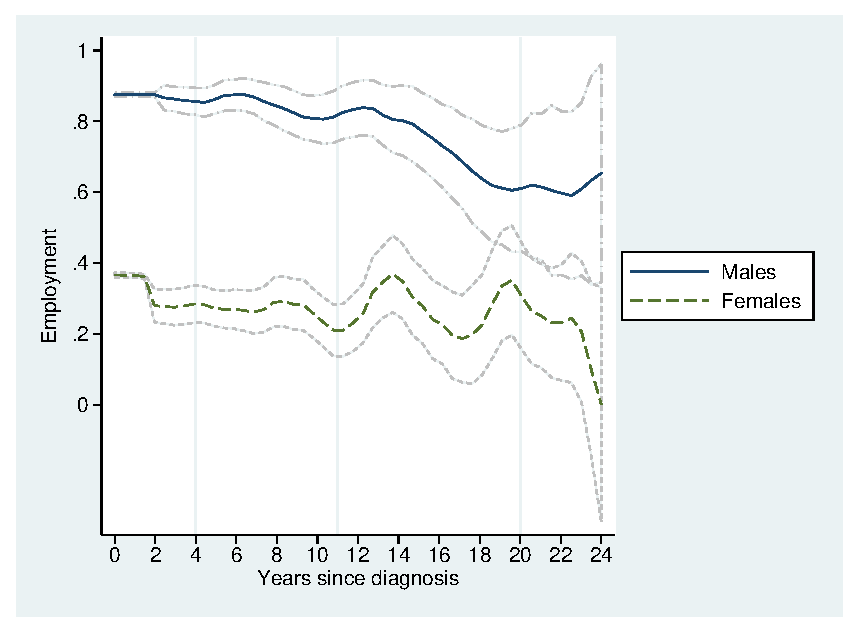
\includegraphics[width=\linewidth]{Chapter4/Figures/lpoly_works_diabetesduration.eps}\\
\footnotesize{\textit{Notes} The dotted lines around the main line show 95\% confidence intervals.}
\end{center}
\end{figure}

\newpage
\begin{figure}[h!]
\caption{\label{fig:Kernel-weighted-local-polynomial_wage}Kernel-weighted local
polynomial regression of log hourly wages on diabetes duration.}%
\begin{center}
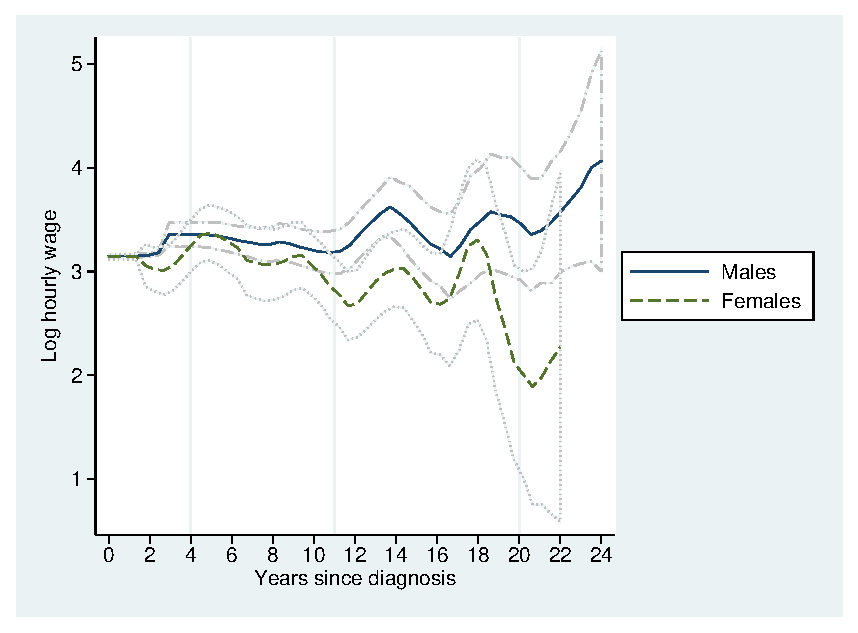
\includegraphics[width=\linewidth]{Chapter4/Figures/lpoly_wage_diabetesduration.eps}\\
\footnotesize{\textit{Notes} The dotted lines around the main line show 95\% confidence intervals.}
\end{center}
\end{figure}

\newpage
\begin{figure}[h!]
\caption{\label{fig:Kernel-weighted-local-polynomial_workhrs}Kernel-weighted local
polynomial regression of working hours on diabetes duration.}%
\begin{center}
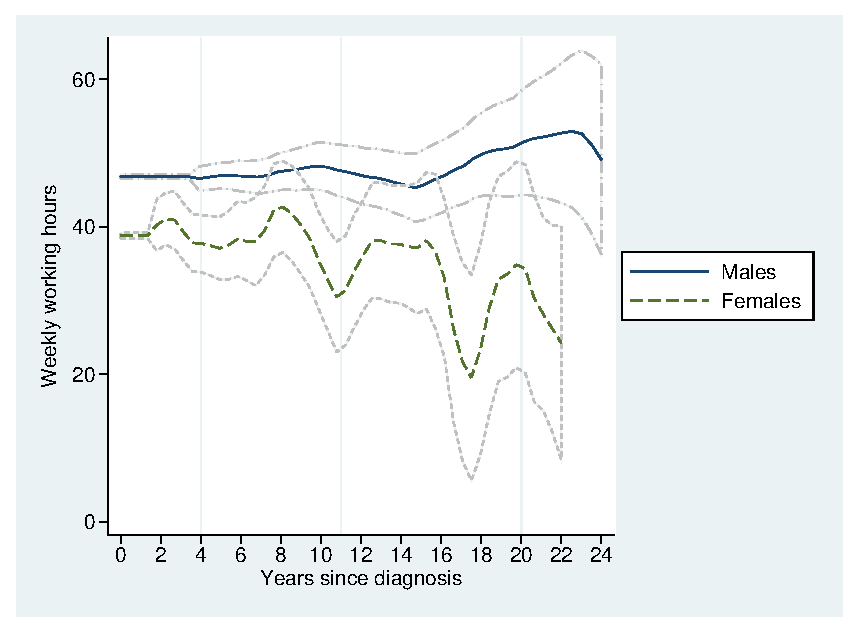
\includegraphics[width=\linewidth]{Chapter4/Figures/lpoly_workhrs_diabetesduration.eps}\\
\footnotesize{\textit{Notes} The dotted lines around the main line show 95\% confidence intervals.}
\end{center}
\end{figure}
\clearpage





\begin{table}[p]
\caption{\label{tab:Self-reported-diabetes-duration_employ}Relationship between self-reported years since diagnosis and employment probabilities using continuous duration and duration splines.}
\begin{center}
%\resizebox{\linewidth}{!}{%
\begin{adjustbox}{max width=\linewidth}
\begin{threeparttable}

{
\def\sym#1{\ifmmode^{#1}\else\(^{#1}\)\fi}
\begin{tabular}{l*{6}{S
S}}
\toprule
                &\multicolumn{3}{c}{Males}                               &\multicolumn{3}{c}{Females}                             \\\cmidrule(lr){2-4}\cmidrule(lr){5-7}
                &\multicolumn{1}{c}{(1)}&\multicolumn{1}{c}{(2)}&\multicolumn{1}{c}{(3)}&\multicolumn{1}{c}{(4)}&\multicolumn{1}{c}{(5)}&\multicolumn{1}{c}{(6)}\\
                  &\multicolumn{1}{c}{OLS}&\multicolumn{1}{c}{OLS}&\multicolumn{1}{c}{FE}&\multicolumn{1}{c}{OLS}&\multicolumn{1}{c}{OLS}&\multicolumn{1}{c}{FE}\\
                                &\multicolumn{1}{c}{(Wave 3)}&\multicolumn{1}{c}{(Pooled)}&\multicolumn{1}{c}{}&\multicolumn{1}{c}{(Wave 3)}&\multicolumn{1}{c}{(Pooled)}&\multicolumn{1}{c}{}\\
\midrule
\addlinespace
Panel A: linear &&&&&&\\
Diabetes duration &   -.008\sym{***}&    -.007\sym{***}&    -.017\sym{***}&    -.005\sym{***}&    -.004\sym{***}&    -.009\sym{*}  \\
                &   (.002)         &   (.002)         &   (.006)         &   (.002)         &   (.001)         &   (.005)         \\

\midrule
                Hausman test    &                  &                  &  153.024         &                  &                  &  200.073         \\
                \hspace*{10mm} p-value         &                  &                  &     .000         &                  &                  &     .000         \\
\midrule
\addlinespace
Panel B: splines&&&&&&\\
Diabetes duration &&&&&&\\
\hspace*{10mm}0--4&    -.007         &    -.007         &    -.026\sym{*}  &    -.010         &    -.015\sym{**} &    -.017         \\
                &   (.007)         &   (.006)         &   (.014)         &   (.007)         &   (.006)         &   (.016)         \\
\hspace*{10mm}5--11&     .000         &    -.003         &    -.003         &    -.004         &     .004         &    -.003         \\
                &   (.009)         &   (.006)         &   (.009)         &   (.008)         &   (.006)         &   (.008)         \\
\hspace*{10mm}12--20&  -.030\sym{**} &    -.017\sym{*}  &    -.029\sym{*}  &     .005         &    -.004         &    -.014         \\
                &   (.012)         &   (.010)         &   (.016)         &   (.008)         &   (.006)         &   (.011)         \\
\hspace*{10mm}> 20&     .011         &     .007         &    -.046\sym{*}  &    -.010\sym{*}  &    -.003         &    -.015         \\
                &   (.016)         &   (.014)         &   (.028)         &   (.006)         &   (.003)         &   (.018)         \\
\midrule
Hausman test    &                  &                  &  161.953         &                  &                  &  198.692         \\
\hspace*{10mm} p-value         &                  &                  &     .000         &                  &                  &     .000         \\
N               &     8217         &    16292         &    16292         &    10467         &    22407         &    22407         \\
\bottomrule
\end{tabular}
\begin{tablenotes}
\item \footnotesize \textit{Notes} The table presents the results of three estimation methods. Panel A presents the results of the linear specifications. Panel B presents the results of the non-linear specifications. Robust standard errors in parentheses. Other control variables: state dummies, urbanization dummies, education dummies, married dummy, number children < 6, wealth, age squared and calendar year dummies. The OLS and pooled OLS models additionally control for age. \sym{*} \(p<0.10\), \sym{**} \(p<0.05\), \sym{***} \(p<0.01\).
\end{tablenotes}
}
\end{threeparttable}
\end{adjustbox}
\end{center}
\end{table}


\begin{table}[p]
\caption{\label{tab:Self-reported-diabetes-duration_wage}Relationship between self-reported years since diagnosis and log hourly wage / weekly working hours using continuous duration and duration splines.}
\begin{center}
%\resizebox{\linewidth}{!}{%
\begin{adjustbox}{max width=\linewidth}
\begin{threeparttable}

{
\def\sym#1{\ifmmode^{#1}\else\(^{#1}\)\fi}
\begin{tabular}{l*{6}{S
S}}
\toprule
                &\multicolumn{3}{c}{Males}                               &\multicolumn{3}{c}{Females}                             \\\cmidrule(lr){2-4}\cmidrule(lr){5-7}
                &\multicolumn{1}{c}{(1)}&\multicolumn{1}{c}{(2)}&\multicolumn{1}{c}{(3)}&\multicolumn{1}{c}{(4)}&\multicolumn{1}{c}{(5)}&\multicolumn{1}{c}{(6)}\\
                &\multicolumn{1}{c}{OLS}&\multicolumn{1}{c}{OLS}&\multicolumn{1}{c}{FE}&\multicolumn{1}{c}{OLS}&\multicolumn{1}{c}{OLS}&\multicolumn{1}{c}{FE}\\
                 &\multicolumn{1}{c}{(wave 3)}&\multicolumn{1}{c}{(pooled)}&\multicolumn{1}{c}{}&\multicolumn{1}{c}{(wave 3)}&\multicolumn{1}{c}{(pooled)}&\multicolumn{1}{c}{}\\
\midrule

                &\multicolumn{6}{c}{\textbf{Log hourly wages}}\\
                \addlinespace
Panel A: linear &&&&&&\\
Diabetes duration&  .001         &     .010\sym{**} &    -.019         &    -.014\sym{*}  &    -.009         &    -.073\sym{**} \\
                &   (.006)         &   (.005)         &   (.018)         &   (.008)         &   (.008)         &   (.029)         \\
\midrule                
Hausman test    &                  &                  &  838.213         &                  &                  &   93.232         \\
\hspace*{10mm} p-value         &                  &                  &     .000         &                  &                  &     .000         \\                
\midrule
\addlinespace
Panel B: splines&&&&&&\\
Diabetes duration&&&&&&\\
\hspace*{10mm}0--4&      .034\sym{*}  &     .046\sym{***}&     .033         &     .027         &     .030         &     .015         \\
                &   (.017)         &   (.016)         &   (.055)         &   (.031)         &   (.026)         &   (.138)         \\
\hspace*{10mm}5--11&    -.041\sym{*}  &    -.037\sym{**} &    -.055\sym{*}  &    -.039         &    -.034         &    -.101\sym{*}  \\
                &   (.021)         &   (.018)         &   (.033)         &   (.030)         &   (.024)         &   (.056)         \\
\hspace*{10mm}12--20&      0.015         &     .044         &     .062         &    -.032         &    -.071\sym{*}  &    -.051         \\
                &   (.033)         &   (.029)         &   (.056)         &   (.042)         &   (.039)         &   (.047)         \\
\hspace*{10mm}> 20&     .053         &     .014         &    -.111         &    -.007         &     .041\sym{***}&    -.204\sym{***}\\
                &   (.054)         &   (.040)         &   (.104)         &   (.028)         &   (.015)         &   (.053)         \\
\midrule
Hausman test    &                  &                  & 1037.290         &                  &                  &   96.266         \\
\hspace*{10mm} p-value         &                  &                  &     .000         &                  &                  &     .000         \\
N               &     5509         &    10767         &    10767         &     2874         &     5741         &     5741         \\
\bottomrule
\addlinespace
&\multicolumn{6}{c}{\textbf{Weekly working hours}}\\
\addlinespace
Panel A: linear &&&&&&\\
Diabetes duration & .069         &     .048         &     .181         &    -.020         &    -.124         &     .208         \\
                &   (.124)         &   (.102)         &   (.330)         &   (.187)         &   (.127)         &   (.652)         \\
\midrule
Hausman test    &                  &                  &  704.904         &                  &                  &  107.709         \\
\hspace*{10mm} p-value         &                  &                  &     .000         &                  &                  &     .000         \\
\midrule
\addlinespace
Panel B: splines &&&&&&\\
Diabetes duration &&&&&&\\
\hspace*{10mm}0--4&      -.033         &    -.233         &     .709         &     .739         &     .470         &    2.014         \\
                &   (.421)         &   (.325)         &   (.938)         &   (.645)         &   (.586)         &  (2.947)         \\
\hspace*{10mm}5--11&  .269         &     .338         &    -.218         &    -.410         &    -.479         &    -.508         \\
                &   (.539)         &   (.399)         &   (.568)         &   (.728)         &   (.553)         &  (1.020)         \\
\hspace*{10mm}12--20&    .209         &     .137         &     .698         &    -.164         &    -.051         &    -.402         \\
                &   (.730)         &   (.538)         &   (.945)         &   (.995)         &   (.700)         &  (1.207)         \\
\hspace*{10mm}> 20&  -1.300         &    -.768         &     .039         &    -.499         &    -.418         &    8.117\sym{***}\\
                &   (.944)         &   (.930)         &  (2.184)         &   (.930)         &   (.305)         &  (1.612)         \\
\midrule
Hausman test    &                  &                  &  724.225         &                  &                  &  112.627         \\
\hspace*{10mm} p-value         &                  &                  &     .000         &                  &                  &     .000         \\
N               &     6807         &    13581         &    13581         &     3591         &     7383         &     7383         \\
\bottomrule
\end{tabular}
\begin{tablenotes}
\item \footnotesize \textit{Notes} The table presents the results of three estimation methods for the two dependent variables: log hourly wages and weekly working hours. Panel A presents the results of the linear specifications. Panel B presents the results of the non-linear specifications. Robust standard errors in parentheses. Other control variables: state dummies, urbanization dummies, education dummies, married dummy, number children < 6, wealth, age squared, calendar year dummies, type of work (agricultural and self employed with dependent non-agricultural wage employment as the base) and health insurance status. The OLS and pooled OLS models additionally control for age. \sym{*} \(p<0.10\), \sym{**} \(p<0.05\), \sym{***} \(p<0.01\).
\end{tablenotes}
}
\end{threeparttable}
\end{adjustbox}
\end{center}
\end{table}

%\FloatBarrier

\subsection{Cross-sectional biomarker analysis}


In this section we gain additional insights from using the biomarker data collected in the
third wave of the \ac{MxFLS}. These data enable us to identify respondents with
\ac{HbA1c} levels equal to or above the internationally recognized diabetes threshold of 6.5\%. This will allow the investigation of the direction of bias introduced when relying on self-reported diabetes only and when it is not possible to identify those unaware as well.

We first present a cross tabulation of self-reported diabetes and the results of the biomarker analysis (Table  \ref{tab:Biomarker_observations}). The table shows that 27\% of the sample have \ac{HbA1c} levels indicative of diabetes and 81\% of those self-reporting a diabetes diagnosis also have \ac{HbA1c} levels equal to or above the diabetes threshold. Overall, of the people with diabetes according to the biomarker analysis, 32\% self-report a diagnosis, while 68\% do not.


\begin{table}[p]
\caption{\label{tab:Biomarker_observations}Number of observations with diabetes (HbA1c $\geq 6.5\%$) and self-reported diabetes.}
\begin{center}
\begin{adjustbox}{max width=\linewidth}
\begin{threeparttable}
{
\def\sym#1{\ifmmode^{#1}\else\(^{#1}\)\fi}
\begin{tabular}{l*{3}{S S}}
\toprule
            &\multicolumn{1}{c}{$HbA1c < 6.5\%$}&\multicolumn{1}{c}{HbA1c $\geq 6.5\%$}&\multicolumn{1}{c}{Total}\\
\midrule
No self-reported diabetes & 4544 & 1181 & 5725 &  \\
 & 79\% & 21\% & 100\% &  \\
& 97\% & 68\% & 89\% &  \\
Self-reported diabetes & 129 & 554 & 683 &  \\
 & 19\% & 81\% & 100\% &  \\
 & 3\% & 32\% & 11\% &  \\
Total & 4673 & 1735 & 6408 &  \\
 & 73\% & 27\% & 100\% &  \\
  & 100\% & 100\% & 100\% &  \\
\bottomrule
\end{tabular}
\begin{tablenotes}
\item \footnotesize \textit{Notes} The first row of each category presents absolute values, the second row presents row percentages and the third row present column percentages.
\end{tablenotes}
}
\end{threeparttable}
\end{adjustbox}
\end{center}
\end{table}

To further investigate the relationship of self-reported and biomarker tested diabetes, we estimate the models presented in equations \ref{eq:diab_sr}, \ref{eq:diab} and \ref{eq:diab_ud}.  
The results in columns 1 and 2 of Table \ref{tab:Biomarker_results} show that the earlier longitudinal results using self-reported diabetes are robust for the biomarker sample. The coefficients in column 3 and 4 indicate that the associations with employment probabilities are much weaker when using diabetes defined by the biomarker instead of self-reported diabetes.\footnote{We also created a dummy variable that additionally to measured diabetes accounted for those with a self-reported diabetes diagnosis but biomarker levels below the diabetes threshold. This allowed us to investigate the effect for the entire diabetes population. The coefficients and their statistical significance are only marginally different to those presented in columns 3 and 4 of Table \ref{tab:Biomarker_results}, which is why we do not present them here.} In columns 5 and 6, obtained from estimating Eq. \ref{eq:diab_ud}, the coefficient for the biomarker diabetes population $Dbio_i$ now reflects the effect of undiagnosed diabetes, as the regression includes a control for self-reported diabetes, revealing that undiagnosed diabetes is not associated with any of the labour market outcomes. 

\newpage
\begin{table}[p]
\caption{\label{tab:Biomarker_results}Biomarker results}
\begin{center}
\begin{adjustbox}{max width=\linewidth}
\begin{threeparttable}
{
\def\sym#1{\ifmmode^{#1}\else\(^{#1}\)\fi}
\begin{tabular}{l*{6}{S
S}}
\toprule
                &\multicolumn{2}{c}{Self-reported diabetes}    &\multicolumn{2}{c}{HbA1c $\geq$ 6.5}&\multicolumn{2}{c}{HbA1c $\geq$ 6.5 and self-reported d.}                 \\\cmidrule(lr){2-3}\cmidrule(lr){4-5}\cmidrule(lr){6-7}
                &\multicolumn{1}{c}{(1)}&\multicolumn{1}{c}{(2)}&\multicolumn{1}{c}{(3)}&\multicolumn{1}{c}{(4)}&\multicolumn{1}{c}{(5)}&\multicolumn{1}{c}{(6)}\\
                &\multicolumn{1}{c}{Males}&\multicolumn{1}{c}{Females}&\multicolumn{1}{c}{Males}&\multicolumn{1}{c}{Females}&\multicolumn{1}{c}{Males}&\multicolumn{1}{c}{Females}\\
\midrule
\multicolumn{7}{l}{\hspace*{10mm}\textbf{Dependent variable: Employment}} \\
Self-reported diabetes&   -.051\sym{**} &    -.044\sym{*}  &                  &                  &    -.053\sym{**} &    -.032         \\
                &   (.026)         &   (.023)         &                  &                  &   (.026)         &   (.026)         \\
HbA1c $\geq$ 6.5&                  &                  &    -.012         &    -.031\sym{*}  &     .003         &    -.022         \\
                &                  &                  &   (.016)         &   (.018)         &   (.017)         &   (.019)         \\
\midrule
N               &\multicolumn{1}{S}{2785}         &\multicolumn{1}{S}{3623}         &\multicolumn{1}{S}{2785}         &\multicolumn{1}{S}{3623}         &\multicolumn{1}{S}{2785}         &\multicolumn{1}{S}{3623}         \\
\midrule
\multicolumn{7}{l}{\hspace*{10mm}\textbf{Dependent variable: Log hourly wages}} \\ 
\addlinespace
Self-reported diabetes&    -.010         &    -.040         &                  &                  &    -.006         &    -.010         \\
                &   (.065)         &   (.113)         &                  &                  &   (.078)         &   (.119)         \\
HbA1c $\geq$ 6.5&                  &                  &    -.007         &    -.057         &    -.006         &    -.055         \\
                &                  &                  &   (.044)         &   (.070)         &   (.049)         &   (.075)         \\
\midrule
N               &\multicolumn{1}{S}{1803}         &\multicolumn{1}{S}{884}         &\multicolumn{1}{S}{1803}         &\multicolumn{1}{S}{884}         &\multicolumn{1}{S}{1803}         &\multicolumn{1}{S}{884}         \\
\midrule
\multicolumn{7}{l}{\hspace*{10mm}\textbf{Dependent variable: Weekly working hours}} \\ 
\addlinespace
Self-reported diabetes&   -.293         &    -.751         &                  &                  &    -.286         &   -1.566         \\
                &  (1.305)         &  (2.178)         &                  &                  &  (1.419)         &  (2.351)         \\
HbA1c $\geq$ 6.5&                  &                  &    -.088         &    1.153         &    -.012         &    1.525         \\
                &                  &                  &   (.844)         &  (1.462)         &   (.925)         &  (1.565)         \\
\bottomrule
\end{tabular}
\begin{tablenotes}
\item \footnotesize \textit{Notes} Community level fixed effects. Robust standard errors in parentheses. Other control variables: age, age squared, state dummies, urbanization dummies, education dummies, married dummy, number children < 6 and wealth. Calender year dummies are included as data collection for the third wave was stretched out over several years. The wage and working hour models additionally control for type of work (agricultural and self employed with non-agricultural wage employment as the base) and for health insurance status. \sym{*} \(p<0.10\), \sym{**} \(p<0.05\), \sym{***} \(p<0.01\).
\end{tablenotes}
}
\end{threeparttable}
\end{adjustbox}
\end{center}
\end{table}


As discussed earlier, differences in effects between self-reported diabetes and those undiagnosed are likely to stem from selection into the diagnosed population, for instance those in worse health, with higher \ac{HbA1c} levels or a longer disease duration are more likely to go to the doctor and be diagnosed as well as to lose their job because of their diabetes. To further explore this, we first estimate models additionally controlling for self-reported health status to capture differences in subjective individual health. Secondly, we estimate models accounting for measured \ac{HbA1c} levels, to  investigate in how far current diabetes severity affects our labour market outcomes. If current severity would be related to labour market outcomes and explain the difference between self-reported and the undiagnosed diabetes population, one would expect an adverse association with increasing \ac{HbA1c} levels, for both self-reporting and undiagnosed. To investigate this, we construct three dummy variables using \ac{HbA1c} groups above the diabetes threshold (i.e. 6.5--7.9, 8--11.9 and 12--14), each for those with self-reported diabetes and for those unaware of their diabetes (Table \ref{tab:Diagnosed_undiagnosed_robust}, Panel B).

\begin{table}[p]
\caption{\label{tab:Diagnosed_undiagnosed_robust}Self-reported diabetes, biomarkers, diabetes severity and self-reported health and their association with labour market outcomes}
\begin{center}
\begin{adjustbox}{max width=\linewidth} 
\begin{threeparttable} 
{
\def\sym#1{\ifmmode^{#1}\else\(^{#1}\)\fi}
\begin{tabular}{l*{6}{S
S}}
\toprule
                &\multicolumn{2}{c}{Employment}       &\multicolumn{2}{c}{Log hourly wages} &\multicolumn{2}{c}{Weekly working hours}\\\cmidrule(lr){2-3}\cmidrule(lr){4-5}\cmidrule(lr){6-7}
                &\multicolumn{1}{c}{(1)}&\multicolumn{1}{c}{(2)}&\multicolumn{1}{c}{(3)}&\multicolumn{1}{c}{(4)}&\multicolumn{1}{c}{(5)}&\multicolumn{1}{c}{(6)}\\
                &\multicolumn{1}{c}{Males}&\multicolumn{1}{c}{Females}&\multicolumn{1}{c}{Males}&\multicolumn{1}{c}{Females}&\multicolumn{1}{c}{Males}&\multicolumn{1}{c}{Females}\\
\midrule
\multicolumn{6}{l}{\hspace*{10mm}\textbf{Panel A (self-reported health)}}\\  
Self-reported diabetes&   -.036         &    -.023         &     .002         &     .060         &     .123         &   -2.191         \\
                &   (.026)         &   (.027)         &   (.079)         &   (.121)         &  (1.433)         &  (2.386)         \\        
Hba1c $\geq 6.5\%$&       .003         &    -.023         &    -.004         &    -.051         &    -.066         &    1.829         \\
                &   (.017)         &   (.019)         &   (.049)         &   (.075)         &   (.926)         &  (1.569)         \\
\multicolumn{6}{l}{Self-reported health status}\\
\hspace*{10mm}good&    .023         &     .057\sym{*}  &     .061         &    -.115         &   -1.131         &    3.521         \\
                &   (.025)         &   (.034)         &   (.074)         &   (.124)         &  (1.376)         &  (2.499)         \\
\hspace*{10mm}fair&    -.007         &     .006         &     .025         &    -.157         &   -1.606         &    4.646\sym{*}  \\
                &   (.026)         &   (.034)         &   (.076)         &   (.128)         &  (1.424)         &  (2.607)         \\
\hspace*{10mm}bad &    -.127\sym{***}&    -.024         &    -.016         &    -.371\sym{*}  &   -6.190\sym{**} &    6.918\sym{*}  \\
                &   (.043)         &   (.046)         &   (.135)         &   (.189)         &  (2.521)         &  (3.858)         \\
\hspace*{10mm}very bad&    -.165         &     .117         &    -.331         &     .316         &   -1.869         &  -17.400\sym{*}  \\
                &   (.110)         &   (.116)         &   (.300)         &   (.439)         &  (6.433)         &  (9.005)         \\
\midrule
N               &\multicolumn{1}{S}{2785}         &\multicolumn{1}{S}{3621}         &\multicolumn{1}{S}{1803}         &\multicolumn{1}{S}{883}         &\multicolumn{1}{S}{2302}         &\multicolumn{1}{S}{1143}         \\
\midrule
\multicolumn{6}{l}{\hspace*{10mm}\textbf{Panel B (HbA1c levels)}}\\
\multicolumn{6}{l}{Self-reported diabetes}\\
\hspace*{10mm}$6.5 - 7.9$&    -.126\sym{**} &    -.040         &    -.228\sym{*}  &     .041         &    1.218         &   -9.170\sym{*}  \\
                &   (.059)         &   (.051)         &   (.127)         &   (.269)         &  (2.921)         &  (4.864)         \\
\hspace*{10mm}$8 - 11.9$&    -.052         &    -.051         &     .026         &     .225         &   -1.332         &   -1.086         \\
                &   (.051)         &   (.042)         &   (.107)         &   (.206)         &  (2.298)         &  (4.395)         \\
\hspace*{10mm}12+  &     .011         &     .021         &    -.106         &    -.427         &    1.979         &   -2.518         \\
                &   (.062)         &   (.069)         &   (.156)         &   (.279)         &  (3.692)         &  (5.335)         \\
\multicolumn{6}{l}{Undiagnosed diabetes}\\
\hspace*{10mm}$6.5 - 7.9$&     .005         &    -.002         &     .015         &    -.040         &    1.003         &    3.616         \\
                &   (.022)         &   (.025)         &   (.058)         &   (.099)         &  (1.178)         &  (2.323)         \\
\hspace*{10mm}$8 - 11.9$&     .006         &    -.027         &     .014         &    -.204         &   -1.004         &    -.077         \\
                &   (.035)         &   (.031)         &   (.078)         &   (.129)         &  (1.485)         &  (2.614)         \\
\hspace*{10mm}12+&     .015         &    -.055         &    -.019         &     .169         &   -1.581         &    1.753         \\
                &   (.040)         &   (.046)         &   (.087)         &   (.181)         &  (2.099)         &  (3.978)         \\
\midrule
N               &\multicolumn{1}{S}{2785}         &\multicolumn{1}{S}{3623}         &\multicolumn{1}{S}{1803}         &\multicolumn{1}{S}{884}         &\multicolumn{1}{S}{2302}         &\multicolumn{1}{S}{1144}         \\
\bottomrule
\end{tabular}
\begin{tablenotes}
\item \footnotesize \textit{Notes} Community level fixed effects. Robust standard errors in parentheses. Other control variables: age, age squared, state dummies, urbanization dummies, education dummies, married dummy, number children < 6 and wealth. Calender year dummies are included as data collection for the third wave was stretched out over several years. The wage and working hour models additionally control for type of work (agricultural and self employed with non-agricultural wage employment as the base) and for health insurance status. \sym{*} \(p<0.10\), \sym{**} \(p<0.05\), \sym{***} \(p<0.01\).
\end{tablenotes}
}
\end{threeparttable}
\end{adjustbox}
\end{center}
\end{table}


When additionally controlling for subjective health status, we find that for men and women the difference between self-reported diabetes and undiagnosed diabetes is reduced due to a smaller coefficient for self-reported diabetes (Table \ref{tab:Diagnosed_undiagnosed_robust}, Panel A). Especially for women, the point estimates for self-reported diabetes and undiagnosed diabetes are now virtually the same size, suggesting that differences could be due to the differences in self-reported health. For men, factors not captured by self-reported health may still play a role. \footnote{Additionally accounting for measures of overweight and obesity, self-reported hypertension, heart disease and depression does not further affect the interpretation of the diabetes coefficient.}

Turning to Panel B, we do not find a consistent relationship of increasing \ac{HbA1c} levels with employment chances, especially for those self-reporting, suggesting that current disease severity may not explain the different employment effects of diabetes for the aware and unaware.

To the best of our knowledge only one study has previously used biomarkers to analyse the relationship with labour market outcomes in a comparable population. \textcite{BrownIII2011} use data for a Mexican American population in a broadly comparable way to this paper, though stopping short of investigating the labour market impact of undiagnosed diabetes. In concordance with our results this study also finds that once diabetes is diagnosed, current management plays a minor role in determining labour market outcomes. This is not surprising given that \ac{HbA1c} levels only provide a picture of blood glucose levels over the last three months. They therefore may not be representative of blood glucose levels in the years before and after the diabetes diagnosis which ultimately determine how soon complications appear and how severe they will be.

\parencite{Minor2015} finds for a general USA population, similar to us, that people with undiagnosed diabetes likely, if at all, experience smaller employment penalties than people self-reporting the disease. He finds, however, much bigger effects then we do when estimating the impact of biometrically measured diabetes instead of distinguishing between the self-reporting and those unaware. This may be explained by the fact that in that study the undiagnosed population made up a much smaller share of the overall diabetes population compared to our study, so that self-reported diabetes was still the predominant factor driving the result.  
%\FloatBarrier


\section{\label{sec:cha_4_conclusion}Conclusion}

Diabetes has become one of the most common chronic diseases in middle- and high-income countries, with the potential to severely impact the health and economic well-being of those directly (and possibly indirectly) affected. Yet there remains only limited 'hard' evidence on the economic consequences, especially for these countries. Moreover, what evidence does exist at best partially tackles the econometric challenges involved. 

This paper improves on existing work by addressing several methodological challenges that arise due to the nature of the disease and types of data available, using rich longitudinal panel data from Mexico, a \ac{MIC} for which the biomarker data used in this paper indicates that diabetes, including undiagnosed diabetes, has reached alarming levels.

Apart from providing unique evidence for a developing country, the paper makes methodological contributions for the estimation of labour market effects of diabetes. By estimating individual fixed effects the analysis provides an improved accounting for the endogeneity of self-reported diabetes, as this allows cancelling out the potential role of unobserved individual traits that may affect both labour market outcomes and propensity to self-report (or suffer from) diabetes. Using further information on the year of diagnosis enables us to investigate the potential heterogeneity in the effect of self-reported diabetes on labour market outcomes over time. Finally, taking advantage of biomarker data to identify the entire diabetes population, i.e. including those with undiagnosed diabetes, allows for an assessment of the potential bias in estimates relying on self-reported diabetes (which is still the most frequent measure in the previous literature).

The first part of our results confirms a considerable gap in employment probabilities for both men and women reporting a diabetes diagnosis, compared to those that do not report the condition. We also find some evidence that diabetes is more likely to reduce the probability of employment in the agricultural and self-employment sector, characterized predominantly by informal arrangements, compared to the rest of the workforce. Those who remain employed do not suffer any wage or labour supply effects, possibly because they are still relatively healthy or are able to resort to a type of work that does not entail their diabetes status limiting their work-related performance. More research will be needed to confirm and further investigate this finding as well as its interpretation. 

Regarding the heterogeneity in the effects of diabetes over time, our results indicate an adverse impact of self-reported diabetes on employment chances, with the impact growing in magnitude especially after the first 10 years post-diagnosis. This is plausible in that as time lived with diabetes evolves, complications associated with diabetes tend to become more frequent and more severe \parencite{Adler2003}. Looking at wages as our labour market outcome, we uncover some adverse effects for females, indicating a sizeable reduction with time since diagnosis. These findings may bode ill for countries \DIFdelbegin \DIFdel{were }\DIFdelend \DIFaddbegin \DIFadd{where }\DIFaddend diabetes has started appearing at an increasingly younger age, causing people to live with the disease for larger parts of their productive lifespan, possibly exacerbating the economic effects of reduced employment due to diabetes \parencite{Hu2011,Villalpando2010}.

The second part of our results indicates that only relying on self-reported diabetes can lead to an overestimation of the relationship between diabetes and labour market outcomes. We find that a negative relationship only exists for those with self-reported, but not for those with undiagnosed diabetes. This perhaps surprising, notable difference, is at least mediated by the subjective health status being worse for those self-reporting compared to the undiagnosed. Current disease severity, as proxied by \ac{HbA1c} levels, does not appear to play an important role in this context.

Our findings bear several implications. First, when interpreting labour market impact estimates relying on self-reported diabetes, one cannot assume that the results extend to those with undiagnosed diabetes. However, the strategy of simply merging self-reported and undiagnosed in one diabetes category may not be ideal either, as doing so will fail to account for the heterogeneity between the groups in the amount of health information they possess, the time they have already been exposed to elevated blood glucose levels and consequently their subjective as well as true health status, leading to a potentially important loss of information. If, by contrast, both groups are separately accounted for in the model, thereby acknowledging their inherent differences, this allows us to gain information about the distribution of the economic burden across the two groups. 

In the case of Mexico, given that more than 7\% of the Mexican population have been diagnosed with diabetes, the identified reduction in employment probabilities for those with self-reported diabetes still amounts to a significant overall economic burden being associated with (diagnosed) diabetes.

Our results add further weight to the case for reducing the incidence and progression of diabetes. On top of the well-documented health benefits, it appears there are considerable potential gains to be had in terms of increasing the productive lifespan of people. This is of particular importance in \acp{LMIC}, where parental health shocks, related job loss and increasing health expenditures can have repercussions across the entire household. Other family members, including children, may be forced to increase their labour supply and to reduce non-health expenditures in order to prevent deterioration of the household's economic situation. This can lead to forgone investments into child education, showcasing the potential for adverse long-term effects of health shocks due to diabetes \parencite{Bratti2014}. Moreover, the large proportion of undiagnosed people indicates that diagnosis---at least in Mexico---happens too late or not at all, thereby significantly reducing the possibility to prevent complications via appropriate treatment and self-management, which has repercussions by increasing the risk of severe complications appearing early. Hence, much of the health and economic burden may be prevented by earlier diagnosis and, given the generally limited success in achieving good control in Mexico, better treatment of those already diagnosed with diabetes. Ultimately of course, there will be a need to invest in the prevention of diabetes cases in the first place. Taxation of sugar sweetened beverages may be one promising way forward \parencite{Colchero2016}, though the long-term effects in terms of diabetes prevention remain to be demonstrated.Diabetes has become one of the most common chronic diseases in middle- and high-income countries, with the potential to severely impact the health and economic well-being of those directly (and possibly indirectly) affected. Yet there remains only limited 'hard' evidence on the economic consequences, especially for these countries. Moreover, what evidence does exist at best partially tackles the econometric challenges involved. 







 \newpage 
\acresetall  %resets all acronyms
\chapter{\label{cha:China} The relationship between diabetes, employment status and behavioural risk factors: An application of marginal structural models and fixed effects to Chinese panel data}
\section*{Pre-amble}

Chapters \ref{cha:Mex1} and \ref{cha:Mex2} provided evidence of the adverse impact of self-reported diabetes on employment probabilities in Mexico. However, if this is also the case in other \acp{MIC} is unclear. Chapter \ref{cha:China} intents to add to this using panel data covering a period of rapid economic transition in China, again estimating the relationship of diabetes and employment status. Moreover, it provides information about the ability of people with diabetes achieving changes in behavioural risk factors important for the prevention of diabetes complications, as studies have shown that smoking cessation and weight loss after a diagnosis can have beneficial effects on blood glucose control and the risk of complications. Importantly, it not only addresses time-invariant unobserved heterogeneity by using individual level fixed effects as in the previous chapter, but also accounts for the potential effects of time-variant confounding by using marginal structural models.

This method is widely applied in epidemiology and able to account for confounding over time, where prior outcomes can affect the current treatment, for example the previous employment status affects the current diabetes status. This potential source of bias has been assumed to not exist in previous studies, but could potentially have biased the estimate of the effect of diabetes on labour market outcomes. This chapter thereby makes several contributions compared to the previous chapters: It provides information about the robustness of the identified relationship of diabetes on employment status by using an alternative estimation strategy in a different setting, thereby also taking into account the potential effect of behavioural risk factors, and it gives first evidence in how far people with diabetes in China are able to change their behavioural risk factors after a diabetes diagnosis.


%}
\acresetall  %resets all acronyms
 \newpage 
\begin{abstract}

A diabetes diagnosis entails important consequences for its recipients. Diagnosed patients obtain health information but also face the challenge of having to manage the condition via lifestyle adjustments, with potential consequences for---among other things---their economic activity. We investigate the causal effect of a diabetes diagnosis on employment status and behavioural risk-factors, two potentially intertwined factors, using longitudinal data from the \acf{CHNS} that cover the years 1997 to 2011. Two complementary statistical techniques---marginal structural models and fixed effects panel estimation---are used for the statistical analysis, and generate very similar results despite their different underlying assumptions. Both strategies find distinct patterns for males and females. They suggest a decrease in female employment probabilities after a diagnosis (over 11 percentage points) and further show that women are mostly unable to positively change their behavioural risk factors by loosing weight and reducing energy intake. Men, however, do not see their employment probabilities affected by diabetes and also respond to a diagnosis by losing weight and reducing energy intake as well as their intake of alcohol in ways that are sustained over time. These results suggest important inequities in the impact of diabetes between sexes in China and point to the potential of reducing behavioural risk factors for women to narrow these inequities.


\end{abstract}


\section{\label{sec:Introduction5}Introduction}

The effect of diabetes on employment status has received relatively little attention in \acp{MIC}, including China. The scarce existing evidence indicates that diabetes can affect labour market outcomes in \acp{HIC}, but also in \acp{MIC} \parencite{Seuring2016}. This is of growing relevance especially with diabetes appearing increasingly earlier in a person's productive lifespan, among others due to increasing obesity at earlier ages. Importantly, once diagnosed, the onset of diabetes, and diabetes complications, strongly depend on the patient's behaviour. Behavioural risk factors like alcohol consumption, smoking, caloric consumption and weight gain are all related to the onset of diabetes as well as ensuing diabetes complications. Research shows for instance that behaviour changes after a diabetes diagnosis can have positive health effects and reduce the risk of subsequent cardiovascular events \parencite{Long2014} and may help in effectively managing blood glucose levels and achieving further treatment goals \parencite{Zhou2016}. Consequently, if these risk factors can be reduced it may be possible to prevent some of the health and economic burden of diabetes. Thus, it seems that a diabetes diagnosis may present an important opportunity to reduce risk factors for diabetes complications \parencite{DeFineOlivarius2015} and hence also reduce the economic burden of diabetes to the individual. This raises the question how diabetes diagnosis affects both labour market outcomes and health behaviour over time.

However, one of the challenges of determining a causal relationship between  diabetes, employment status and changes in behavioural risk factors is their potential bidirectional interrelatedness. For example, employment status might by affecting weight status by reducing the time spend on physical activity due to reductions in available leisure time, or it may promote risk factors such as smoking behaviour or energy intake that can both affect the probability of developing diabetes as well as diabetes related complications, for instance by increasing stress levels. In an effort to  investigate the dynamic impact of unemployment on health behaviours, \textcite{Colman2014} found heterogeneous effects of unemployment which led to slight weight gain, a decrease in smoking and decreases in fast-food consumption. Macroeconomic evidence also indicates that job loss can lead to changes in health, especially in mental health \parencite{Charles2008}, which may have further downstream effects on health behaviours.

Research on the impact of diabetes on labour market outcomes has so far ignored the potentially simultaneous relationship of diabetes with employment and behavioural diabetes risk factors. Using regression techniques such as \ac{OLS} or \ac{FE} it was assumed that the investigated independent variables are unaffected by prior values of the dependent variable. However, if prior changes in employment status are causally related to a diabetes diagnosis or affect the risk factors for diabetes complications, not accounting for this can lead to biased estimates.\footnote{One solution is to include lagged values of the dependent variable on the right hand side, but this raises challenges of its own, including difficulty of interpretation, but also potentially biased estimates. The lagged dependent variable will be correlated with the time-invariant part of the error-term, violating the assumption of exogeneity of the right-hand side variables. Further, if the other covariates are correlated with the lagged-dependent variable, they will also be biased \parencite{Anderson1982,Nickell1981}.} Similarly, studies investigating the impact of a diabetes diagnosis on behavioural risk factors while not taking into account the effect of employment status on both diabetes and these risk factors, may produce biased estimates. Moreover, apart from time-varying confounding due to observed covariates, unobserved variables present a further challenge. In particular, time-invariant confounders---such as poor early life conditions or personal trades---may simultaneously increase the probabilities to develop diabetes, to be unemployed and to engage in unhealthy behaviour. 

The goal of this study is therefore to assess the impact of a diabetes diagnosis on both employment probabilities and behavioural risk factors while accounting for the potentially intertwined relationships between diabetes, employment and health behaviours. This is done via the use of \acp{MSM}, an estimation strategy that is increasingly common in epidemiology and is able to account for time-dependent confounding across time \parencite{Robins2000} when estimating the impact of a treatment, here a diabetes diagnosis, on the outcome of interest. This is, by our knowledge, the first time this estimation strategy is used to estimate the impact of diabetes on an individual's employment status or behavioural risk factors. We complement this strategy and test the robustness of the \ac{MSM} estimates to the potential violation of one of its crucial assumptions, namely that there are no unmeasured confounding factors. To do this, we compare them with \ac{FE} models which, although unable to account for the potentially bidirectional relationship, do account for unobserved time-invariant confounding factors in addition to confounding due to observed variables. Very different results to the \ac{MSM} would suggest a violation of the assumption of no unobserved confounding. To further investigate and understand the role of confounding factors, we also estimate \ac{RE} models and compare the results.  We thereby further extends the evidence base for the impact of diabetes on labour market outcomes in \acp{MIC}, where currently empirical information is only available for Mexico \parencite{Seuring2016}. At the same time the study provides, as far as we are aware, the first longitudinal evidence for the effect of a diabetes diagnosis on behavioural risk factors in any \acp{LMIC}  country.

 
More information about the effects of a diabetes diagnosis may be particularly important for \acp{LMIC} such as China, where diabetes prevalence has surged from 1\% in the early 1980s to about 10\% in recent years \autocite{Hu2011,Risk2016}. Confronting this diabetes epidemic puts a strain on healthcare systems \parencite{Seuring2015a}, increasing the need to find highly cost-effective prevention and treatment options applicable in \acp{MIC} \parencite{WHOresearchpriorities2010}. However, to do this it is important to assess how successful people with diabetes currently are in preventing adverse economic effects and reducing their risk factors for diabetes complications.


%Finally, another study on China also used diabetes biomarkers to identify those formally unaware of their diabetes, assuming that they were informed about their diabetes status by the survey team \parencite{Liu2014}. They use a difference in difference approach to identify the effect of a diagnosis on labour income in the wave after diagnosis, finding a decrease of about 16\%. They attribute this effect to the psychological consequences of the diabetes diagnosis, however, they are not able to rule out an effect of a deterioration of health on income. Further, the results only provide a short term picture, and it remains unclear if people are able to recover from the initial shock. ONLY INCLUDE IF I ALSO LOOK AT INCOME


The literature trying to identify a causal relationship between diabetes and employment has relied on \ac{IV} strategies \parencite{Brown2005,Latif2009,Seuring2015} and individual \ac{FE} models \parencite{Seuring2016}. However, while an \ac{IV} approach could potentially account for all forms of confounding, the validity of the instruments used is at least questionable (see discussion in Chapter \ref{cha:Mex2}). The \ac{FE} model, as discussed above, also relies on important assumptions that may be violated. Turning to the relationship between a diabetes diagnosis and behavioural risk factors, only one study has intended to causally relate a recent diabetes diagnosis with changes in health behaviours, finding positive behaviour changes shortly after diagnosis in a USA population. The found effects were mostly short lived and tended to dissipate over time, particularly considering weight loss \parencite{Slade2012}. To isolate the causal effect \textcite{Slade2012} created an 'at risk' control group without diabetes that was intended to be similar to the treatment group with diabetes, apart from not having received a diagnosis. He used information on diabetes biomarkers to estimate the propensity score of those without a diabetes diagnosis to be above a specific at risk threshold, so that everybody above a certain propensity score was used to form the control group. He then estimated dynamic population average models, including the lagged dependent variable on the right hand side, as well as \ac{FE} models to identify a causal relationship. While this approach likely improves the control group by increasing its similarity in the diabetes risk profile to the diagnosed population, the use of a lagged dependent variable may have biased the estimates due to unobserved time-invariant variables being correlated with the lagged dependent variable, violating the exogeneity assumption and potentially introducing bias in the other covariates. This is also true for the \ac{FE} model \parencite{Nickell1981,Anderson1982}. Further, the study did not account for employment status as one of the control variables. 

A different identification approach was used by \textcite{Zhao2013a} when investigating the effects of a hypertension diagnosis on nutritional outcomes in China. They used a regression-discontinuity design and biomarker information on blood pressure. A crucial assumption in that study was that people above the hypertension threshold were indeed informed about their hypertension while those just below the threshold were not. These two groups were then compared to isolate the particular effect of the additional health information on food consumption in the following wave. The results indicated that a diagnosis leads to reductions in fat consumption, but no other nutritional outcomes, and only for those economically better off. Several caveats exist for this study and the used approach. According to \textcite{Zhao2013a}, it was not always clear to what extent participants \DIFdelbegin \DIFdel{where }\DIFdelend \DIFaddbegin \DIFadd{were }\DIFaddend informed about their hypertension status and whether they had received just the actual blood pressure measurement information, leaving the interpretation to the participants, or whether they were made explicitly aware of their hypertension (or also pre-hypertension) status. Further, the results may have limited generalisability, since the measured treatment effect \DIFdelbegin \DIFdel{was }\DIFdelend \DIFaddbegin \DIFadd{may have been }\DIFaddend a very local one, \DIFdelbegin \DIFdel{applying only }\DIFdelend \DIFaddbegin \DIFadd{depending on the representativeness of the population distribution below and above the threshold of the overall population above the threshold. In the case of significant differences between the populations, the results would only be applicable }\DIFaddend to the population around the hypertension threshold. Finally, the study only provides information for a relatively short period until the first wave after diagnosis, unable to capture any changes further away from the point of diagnosis. 

Accordingly, there is a need to provide new evidence on the effects of a diabetes diagnosis on employment status as well as behavioural risk behaviours that could affect the development of diabetes complications, using longitudinal data and alternative estimation strategies. Thereby this study adds in several ways to the existing literature. First, it shows the impact of diabetes diagnosis on labour market outcomes in China, not only over the short term, but for a period covering the entire decade of the 2000s, allowing for a more long term investigation of the effects. This both confirms and extends earlier evidence for other settings and using different methods. Second, it provides information on the effect of a diabetes diagnosis on health behaviours. Third, by considering the effects over time on both employment and health behaviour, the results shed light on potential pathways through which the impact on employment may work.  Fourth, the study provides a methodological innovation by using both \ac{MSM} and \ac{FE} estimation methods, offering insights not only on the robustness of the \ac{MSM} results, but also on the validity of some of its assumptions.  


\section{\label{sec:Methods5}Methods}

\subsection{Study sample}


The \acf{CHNS} is an international collaborative project, led by the Carolina Population Center at the University of North Carolina at Chapel Hill, investigating nutrition and health behaviours in nine provinces of China \parencite{Zhang2014d}. We use data from 1997 onwards, which was the first time survey participants provided diabetes information. In total we use six waves (1997, 2000, 2004, 2006, 2009 and 2011) obtained from the longitudinal dataset released in 2015. The data provide extensive information on nutrition and health\DIFdelbegin \DIFdel{, including }\DIFdelend \DIFaddbegin \DIFadd{. Importantly this includes }\DIFaddend anthropometric measures of weight and height \DIFdelbegin \DIFdel{, reducing }\DIFdelend \DIFaddbegin \DIFadd{that reduce }\DIFaddend potential measurement issues \DIFaddbegin \DIFadd{plaguing self-reported data}\DIFaddend . It further provides socioeconomic information, most importantly for this study about employment. The sample is limited to the adult population aged 18--64.  The sample is not nationally representative and as such does not provide sampling weights  \parencite{Popkin2010}.

Overall, between 84\% to 90\% of the survey participants were followed up in the consecutive wave, with attrition being highest after 2006. Attrition in the \ac{CHNS} due to mortality was around 1\% \parencite{Popkin2010}. Other reasons mentioned by \textcite{Popkin2010} are loss in follow up due to migration, natural disasters and redevelopment of housing in the urban centres leading to relocations. We investigated whether any of our variables of interest was significantly related to attrition at any wave. Lower calorie consumption and being unemployed were associated with attrition. Further, attrition was strongly related to urbanization, a higher level of education, being of younger age and having lower family income, suggesting that mostly participants of younger age, more urbanized but from less well-off households tended to leave the survey. Having diabetes was not related to attrition. Attrition rates between the waves are shown in Table \ref{tab:attrition} in the appendix.


\subsection{Assessment of diabetes}

We used self-reported information on a diabetes diagnosis to construct our diabetes indicator. We only relied on incident cases of self-reported diabetes, excluding individuals with self-reported diabetes at baseline. Given the chronic nature of diabetes, we assumed that after the initial diagnosis diabetes persists for the rest of one's life. This is a reasonable assumption given the medical evidence \parencite{Steven2016}.\footnote{Recently, a study showed successful remission of at least 6 months in some patients after the initiation of a very low-calorie diet \parencite{Steven2016}. However, while this shows that type 2 diabetes may be reversible, this cannot be expected for patients diagnosed and currently treated in any healthcare system.} To construct a measure of diabetes duration for incident cases we used self-reported information on the year of diagnosis. If we found that the year of diagnosis was reported to be before the last wave without a reported diagnosis or if the year of diagnosis was not reported, we used the midpoint between the last wave without diagnosis and the first wave with a diagnosis as the year of diagnosis.\footnote{The number of observations replaced at each wave was: 21 (2000), 44 (2004), 51  (2006), 78 (2009), 59 (2011). Overall it affected 43\% of the self-reports of the year of diagnosis.}

\subsection{Assessment of outcomes}

The economic outcome of interest is employment status, and is measured through self-reported response stating whether the respondent is currently working. Respondents who reported not to be working because they were students are excluded, while those who are not working for any other reason, such as doing housework, being disabled or being retired, were included. 

The behavioural risk factor outcomes we estimate are current smoking status, if alcohol was consumed equal to or more than three times per week\footnote{We also estimated models investigating alcohol cessation instead of alcohol reduction, suggesting very similar effects.}, \ac{BMI}, waist circumference in centimetres and daily calorie consumption. Smoking status and alcohol consumption are self-reported, while \ac{BMI} and waist circumference are based on anthropometric measurements, minimizing potential reporting errors and indirectly indicating dietary and activity behaviour. Waist circumference is reported in centimetres. Finally, daily calorie consumption is a constructed variable, available in the \ac{CHNS}, based on the average daily consumption of carbohydrates, protein and fat of every individual in the survey, measured on three consecutive days. As robustness tests, we also considered binary overweight and obesity indicators instead of the continuous \ac{BMI} and waist circumference variables. We applied thresholds suggested by the China Obesity Task Force of a \ac{BMI} $\geq$ 24 to define overweight and a \ac{BMI} $\geq$ 28 to define obesity \parencite{group2004body}. Since there is considerable discussion about the correct thresholds to use for Asian populations to define overweight and obesity \parencite{WHO2004,He2015,Zeng2014a}, we do not include these results in our main analysis but report them in the appendix (page \pageref{tab:obesity_binary}). 


\subsection{Statistical analysis}


Our analysis focuses on two statistical approaches to account for potential confounding and selection bias: \acfp{MSM} and \acf{FE}. Additionally, also \ac{RE} models are estimated.

\subsubsection{Marginal structural models}

\acp{MSM} apply \DIFdelbegin \DIFdel{inverse probability weights }\DIFdelend \DIFaddbegin \acp{IPTW} \DIFaddend to adjust for confounding and selection bias as a result of time-varying confounders being affected by prior exposure to the treatment \DIFdelbegin %DIFDELCMD < \autocite{Robins2000}%%%
\DIFdelend \DIFaddbegin \parencite{Robins2000}\DIFaddend . Under the assumptions of the \ac{MSM}  \DIFdelbegin %DIFDELCMD < \autocite{Robins2000}%%%
\DIFdelend \DIFaddbegin \parencite{Robins2000}\DIFaddend ---the reported treatment is the treatment that has actually been received (consistency), there are no unmeasured confounders (exchangeability) and every person in the sample has a non-zero chance of receiving the treatment (positivity) (see the Discussion section for a discussion of the validity of these assumptions in our case)---the causal \ac{DAG} shown in Figure \ref{fig:DAG_msm} displays the association between confounders and outcomes and a diabetes diagnosis.

In our context it seems possible that, for example, \ac{BMI} could affect the probability of being diagnosed with diabetes which then itself may affect subsequent \ac{BMI} levels, confounding the relationship between a diabetes diagnosis and \ac{BMI} due to non-random selection. Similarly, employment history and current employment could affect the probability of a diabetes diagnosis through their impact on lifestyle and hence diabetes risk factors. For example, an increase in disposable income or a reduction in leisure time as a result of a new job and the subsequent effect on risk behaviours \DIFdelbegin \DIFdel{. }\DIFdelend such as weight gain or higher alcohol consumption, could confound the relationship between a diabetes diagnosis and employment status. \ac{MSM} accounts for this by calculating inverse probability weights based on the potential risk of a person being diagnosed at each point in time, estimated by logistic regression. 

\DIFdelbegin \DIFdel{To calculate these weights we first construct unstabilized weights using baseline values of }\DIFdelend \DIFaddbegin \DIFadd{For the estimation of }\acp{MSM}\DIFadd{, first }\textit{\DIFadd{unstabilized}} \acp{IPTW} \DIFadd{for being diagnosed with diabetes are calculated for each individual at each wave. The }\acp{IPTW} \DIFadd{are proportional to the inverse of the probability of a person having her own observed exposure through that wave and allow the creation of a pseudo population that is exchangeable with the study population within the levels of confounders }\parencite{Cole2008}\DIFadd{. The }\textit{\DIFadd{unstabilized}} \acp{IPTW} \DIFadd{are calculated using }\DIFaddend time-variant confounders \DIFdelbegin \DIFdel{, time-invariant confounders as well as }\DIFdelend \DIFaddbegin \DIFadd{measured at baseline, }\DIFaddend time-variant confounders lagged by one period \DIFaddbegin \DIFadd{and time-invariant confounders as right-hand side variables used }\DIFaddend to predict the \DIFaddbegin \DIFadd{cumulative }\DIFaddend probability of developing diabetes at each wave. We use lagged time-variant confounders to make sure that the predictors of diabetes were determined \DIFdelbegin \DIFdel{before the current diabetesstatus, because current diabetes status as reported in the survey was determined at some point between }\DIFdelend \DIFaddbegin \DIFadd{previous to the manifestation of diabetes. Otherwise, because }\DIFaddend the \DIFdelbegin \DIFdel{current and the previous wave. 
The predictors used are }\DIFdelend \DIFaddbegin \DIFadd{diagnosis happened at an unknown point of time between two waves, the key assumption that the time-variant variables used to predict the probability of a diabetes diagnosis are are determined before the diabetes diagnosis may have been violated. 
}

\DIFadd{The }\textit{\DIFadd{unstabilized}} \acp{IPTW} \DIFadd{are calculated using the following predictors: }\DIFaddend age and age squared to account for changes in risk with increasing age\DIFdelbegin \DIFdel{, }\DIFdelend \DIFaddbegin \DIFadd{; }\DIFaddend an index of urbanization pre-constructed within the \ac{CHNS} data, ranging from 1 to 120 as the level of urbanization increases \parencite{Zhang2014d}, to account for the impact of urbanization on diabetes risk \parencite{Attard2012}\DIFdelbegin \DIFdel{. We also use }\DIFdelend \DIFaddbegin \DIFadd{; }\DIFaddend binary variables for secondary and university education, being married, having any medical insurance, being of Han ethnicity, living in a rural area, the different Chinese regions and the respective survey waves\DIFdelbegin \DIFdel{as predictors. Moreover, we use }\DIFdelend \DIFaddbegin \DIFadd{; }\DIFaddend inflation adjusted per-capita household income to adjust for any effects of household wealth on diabetes\DIFdelbegin \DIFdel{. Finally, all outcome variables (}\DIFdelend \DIFaddbegin \DIFadd{; and }\DIFaddend employment status, alcohol consumption, smoking status, \ac{BMI}, waist circumference and average daily calorie consumption\DIFdelbegin \DIFdel{) are used as predictors. For each wave after the first wave in which each person participated}\DIFdelend \DIFaddbegin \DIFadd{. To create }\acp{IPTW} \DIFadd{that account for each individual's entire reported history of diabetes risk factors}\DIFaddend , cumulative probabilities of diabetes were calculated by multiplying the \DIFaddbegin \DIFadd{predicted }\DIFaddend probabilities in the current and all previous waves, \DIFdelbegin \DIFdel{thus accounting for each individual's entire reported history of diabetes risk factors}\DIFdelend \DIFaddbegin \DIFadd{for each waver after the baseline wave}\DIFaddend .\footnote{To calculated the inverse probability weights we followed the Stata code provided by \textcite{Fewell2004}.}


\begin{figure}[!p]
\begin{center}
\caption{\label{fig:DAG_msm} Direct acyclic graph for the marginal structural model}
\includegraphics[width=\linewidth]{Chapter5/DAG/dag_msm_alt}
\end{center}
\footnotesize{\textit{Notes} \acp{MSM} assume the absence of unobserved time-invariant and unobserved time-variant confounders but allow the past treatments to affect the current outcomes  (arrows going from Diabetes to time-variant covariates in the same wave) and the past outcomes to affect the current treatment (arrows going from time-variant covariates to Diabetes).  Lagged time-variant covariates, baseline and time-invariant covariates predict current diabetes status.}
\end{figure}


Because \DIFdelbegin \DIFdel{unstabilized weights }\DIFdelend \DIFaddbegin \textit{\DIFadd{unstabilized}} \acp{IPTW} \DIFaddend can be highly variable \DIFaddbegin \DIFadd{and therefore less precise}\DIFaddend , it is recommended to stabilize the weights \parencite{Cole2008}. \DIFdelbegin \DIFdel{Using the unstabilized weights as the denominator, stabilized weights }\DIFdelend \DIFaddbegin \DIFadd{To calculate }\textit{\DIFadd{stabilized}} \acp{IPTW}\DIFadd{, }\acp{IPTW} \DIFadd{are created by predicting the diagnosis of diabetes using only baseline values of time-variant and time-invariant confounders as right-hand side variables. Similar to the calculation of }\textit{\DIFadd{unstabilized}} \acp{IPTW}\DIFadd{, cumulative probabilities }\DIFaddend are calculated by \DIFdelbegin \DIFdel{dividing the denominator by the predicted treatment propensity from a model using only time-invariant confounders and baseline information of the time-variant confounders as predictors}\DIFdelend \DIFaddbegin \DIFadd{multiplying the predicted probabilities in the current and all previous waves, for each waver after the baseline wave. To calculate }\textit{\DIFadd{stabilized}} \acp{IPTW} \DIFadd{the just created weights are divided by the }\textit{\DIFadd{unstabilized}} \acp{IPTW}\DIFadd{. The resulting }\textit{\DIFadd{stabilized}} \acp{IPTW} \DIFadd{now only reflect the confounding due to the time-varying covariates, which cannot be appropriately adjusted for by standard regression models }\parencite{Cole2008}\DIFaddend . Because our analysis is stratified by males and females, we create \DIFdelbegin \DIFdel{weights separately for both groups}\DIFdelend \DIFaddbegin \DIFadd{separate weights for each gender}\DIFaddend .

The \acp{MSM} \DIFdelbegin \DIFdel{are estimated using }%DIFDELCMD < \ac{OLS} %%%
\DIFdel{for the continuous outcomes }\DIFdelend \DIFaddbegin \DIFadd{for any of the outcome variables are then estimated adjusting for any baseline and time-invariant confounders used in the calculation of the }\acp{IPTW}\DIFadd{, except for the respective outcome of interest, and weighted by the }\textit{\DIFadd{stabilized}} \acp{IPTW} \DIFadd{to adjust for time-variant confounding. }\ac{OLS} \DIFadd{regression models were used for continuous outcomes (}\ac{BMI}\DIFadd{, waist circumference and calorie consumption) }\DIFaddend and a logistic model for the binary outcomes \DIFaddbegin \DIFadd{(employment status, smoking status and alcohol consumption)}\DIFaddend . For the logistic model we calculate average marginal effects for greater comparability with the results of the \ac{FE} models. \DIFdelbegin \DIFdel{All models are weighted by the stabilized weights constructed beforehand while adjusting for all baseline and time-invariant covariates used in the calculation of the stabilized weights, except for the respective outcome of interest. }\DIFdelend Robust standard errors to account for intra-class correlation of repeated outcome measurements in individuals are used throughout. In our primary analysis, we present the results of the \ac{MSM} with untruncated stabilized weights, as these provide theoretically unbiased estimates, albeit they \DIFdelbegin \DIFdel{likely are }\DIFdelend \DIFaddbegin \DIFadd{may be }\DIFaddend less efficient than truncated weights \DIFaddbegin \DIFadd{if the }\acp{IPTW} \DIFadd{have a wide range considerably diverting from 1 }\DIFaddend \parencite{Cole2008}. \DIFdelbegin \DIFdel{The distribution of the inverse probability weights supports this decision as there are no }\DIFdelend \DIFaddbegin \DIFadd{Given that our }\acp{IPTW} \DIFadd{do not include very }\DIFaddend extreme values and \DIFdelbegin \DIFdel{the mean weight is }\DIFdelend \DIFaddbegin \DIFadd{have a mean weight of }\DIFaddend 1 (see Table \ref{tab:stabweights})\DIFaddbegin \DIFadd{, using untruncated weights likely leads to very little loss in efficiency in our case, supporting the decision to use untruncated weights in our primary analysis}\DIFaddend .

\subsubsection{Fixed effects}

While the \ac{MSM} can account for pre-treatment selection on observable and time-variant confounders, it assumes that there are no unobserved time-invariant confounders such as family background, cognitive abilities, and other personal characteristics. This is a strong assumption that might be violated in practice. The individual level \ac{FE} model can help remedy this problem as it is able to account for both observed time-variant and invariant variables as well as time-invariant unobserved variables as shown in the \ac{DAG} in Figure \ref{fig:DAG_fe}. It does so by demeaning all covariates at each time point with the overall individual mean across all observed time points. It then uses solely the within-person variation for identification, thereby accounting for any time-invariant observed or unobserved as well as observed time-variant effects. 


This comes at a price: due to the demeaning, time-invariant variables, such as Han ethnicity, are dropped from the model and their association with the outcomes cannot be estimated. Further, because the \ac{FE} model is not able to account for any effects of a diabetes diagnosis on other time-variant confounders, only a more limited set of confounders can be included compared to the \ac{MSM}. Otherwise the estimates of the effect of a diabetes diagnosis would likely be biased due to the inclusion of 'bad controls'. Bad controls are control variables that have been affected by the treatment itself---such as \ac{BMI} or smoking status after a diabetes diagnosis---and therefore likely capture part of the causal effect of diabetes on the outcome of interest, biasing the diabetes coefficient \parencite{Angrist2009a}. Also age is dropped from our \ac{FE} estimations because in \ac{FE} models two or more variables that change at the same rate between waves cannot be separately identified. In our case this applies for age and time-dummies, as both variables increase by one unit each additional year \parencite{Wooldridge2012}. Consequently, for the estimation of the effect of time since diagnosis, we have to rely on the presence of people without diabetes in the sample, for which diabetes duration does not increase at the same rate as time. Our \ac{FE} specifications thus only include controls for age squared, the level of urbanization, education, being married, having any medical insurance, living in a rural area, region and time dummies as well as per capita household income.  \ac{FE} models also make another assumption, which has received much less attention, namely that there is no dynamic causal relationship between treatment and outcomes, i.e. that past treatments have no direct effect on current outcomes, and that past outcomes have no direct effect on current treatment. If this assumption is violated, then results based on \ac{FE} are biased \parencite{Imai2016}. Accordingly, the choice between the use of a \ac{FE} model or a \ac{MSM} depends on the trade-off between unobserved time-invariant confounding and dynamic causal relationships between diabetes and our outcome variables.\footnote{Because it is not possible to retrieve average marginal effects from a logistic \ac{FE} model, we prefer to use a linear \ac{FE} model instead. It generally produces very similar estimates compared to non-linear models \parencite{Angrist2009a}.}


\begin{figure}[!p]
\begin{center}
\caption{\label{fig:DAG_fe} Direct acyclic graph for the fixed effects model}
\DIFdelbeginFL %DIFDELCMD < \includegraphics[width=\linewidth]{Chapter5/DAG/dag_fe_alt}
%DIFDELCMD < %%%
\DIFdelendFL \DIFaddbeginFL \includegraphics[width=\linewidth]{Chapter5/DAG/dag_fe_alt_corrections}
\DIFaddendFL \end{center}
\DIFdelbeginFL %DIFDELCMD < \footnotesize{\textit{Notes} \ac{FE} models account for time-invariant unobserved confounding (light grey circle), but still assume the absence of unobserved time-variant confounding. They further do not allow for past outcomes to affect the current treatment, i.e. diabetes status. }
%DIFDELCMD < %%%
\DIFdelendFL \DIFaddbeginFL \footnotesize{\textit{Notes} \ac{FE} models account for time-invariant unobserved confounding (light grey circle), but still assume the absence of unobserved time-variant confounding. They further do not allow for past outcomes to affect the current treatment, i.e. diabetes status.}
\DIFaddendFL \end{figure}


\subsubsection{Random effects}

Random effects assume, similar to the \ac{MSM}, no unmeasured confounding and, similar to the \ac{FE} model, no dynamic relationship between diabetes and our outcomes. Under these assumptions the \ac{RE} model is efficient and consistent, making it the preferable estimator if its assumptions are not violated. It is also preferable over the pooled \ac{OLS} estimator, as the \ac{RE} estimator takes into account the serial correlation of the errors across time \parencite{Wooldridge2012}. 

To discriminate between the \ac{RE} and \ac{FE} estimator, a robust Hausman test is carried out using the user written Stata command xtoverid. A rejection of the null hypothesis suggests that the underlying \ac{RE} assumptions are false and the \ac{FE} model should be used instead \parencite{Wooldridge2012}.\footnote{We use the original non-imputed data to carry out the Hausman test.} 



\subsubsection{Multiple imputation}

To avoid excluding participants with missing data on one or more variables, we used chained multiple imputation to impute the missing values in Stata 13 using the user written ICE command \parencite{Royston2009}. \DIFdelbegin \DIFdel{Overall, thirty imputed datasets were created}\DIFdelend \DIFaddbegin \DIFadd{For most of the included variables, less than 10 percent of the observations was missing. Only the anthropometric measures of }\ac{BMI} \DIFadd{and waist circumference had both about thirteen percent missing data which had to be imputed (see Table \ref{tab:missing_data} in the appendix for detailed information on the number of missing observations). In total---before imputation---close to 20 percent of all cases were incomplete, i.e. had at least one variable that had missing data. Therefore thirty imputations were performed to ensure efficiency and correct standard errors. This is well above the commonly suggested rule of thumb that the number of imputations should be similar to the percentage of incomplete cases in the data (see for example } \textcite{White2011,Bodner2008} \DIFadd{for practical suggestions regarding the optimal number of imputations)}\DIFaddend . Imputation models included all variables used in the \acp{MSM}. We imputed missing data in the same wave for which some data were recorded; we did not impute completely missing waves. Further, we assumed that once a diabetes diagnosis was reported, the individual had diabetes in every ensuing wave, even when the observation was missing. If diabetes was never reported in any wave, we assumed that the individual never had diabetes. We then only imputed missing values for those observations that had a non-missing diabetes status. For the calculation of the marginal effects in the \ac{MSM} logit models, Rubin's rules were applied using the user written Stata command mimrgns \parencite{Klein2014}.

\subsubsection{Numbers of observations}

Because we used lagged independent variables to construct the stabilized weights for the \acp{MSM}, the number of observations used in the \acp{MSM} is lower than those used in the \ac{FE} and \ac{RE} models, where we do not use lagged variables. The summary statistics shown in Table \ref{tab:descriptives_diab} are based on the observations used in the \ac{FE} models. The number of observations is stated below each table.

\subsubsection{Sensitivity analyses}

We conduct three additional sensitivity analyses in order to test the robustness of our results. First, we truncate weights at the 1\textsuperscript{st} and 99\textsuperscript{th} percentile to investigate the sensitivity of the \acp{MSM} to the most extreme weights. While untruncated weights provide unbiased estimates under the assumptions of the \ac{MSM}, they may not be the most efficient and tend to have larger standard errors \parencite{Cole2008}. Second, we estimate the \ac{FE} and \acp{MSM} using the original non-imputed data to ascertain the extent to which multiple imputation affected the results. Third, we report in the appendix the estimates of models using overweight and obesity instead of \ac{BMI} and waist circumference as the outcomes of interest, to investigate the effect of a diabetes diagnosis on changes in the probabilities to be overweight or obese.

\section{\label{sec:Results5}Results}

From the descriptive statistics (Table \ref{tab:descriptives_diab}), we can observe that people with diabetes in any wave are less likely to be employed. Looking at health behaviours, the prevalence of smoking and drinking is lower for men with diabetes; they also consume fewer calories compared to men without diabetes.  Note that it is mainly men who smoke and report alcohol consumption while very few women do so. Further, the diabetes group has both higher \ac{BMI} and waist circumference levels. They are also older, live in more urbanized areas, are more likely to have insurance and men are somewhat better educated while women are less educated compared to their counterparts without diabetes. Both men and women with diabetes report an average time since diagnosis of around 4.5 years. Looking at per capita household income, men and women with diabetes come from household with higher income levels than those without a diabetes diagnosis. Further, it appears that in China it is less educated women that report a diagnosis, while men with diabetes are better educated compared to those without diabetes.

Predicting the denominator for the stabilized weights (Table \ref{tab:predictors}) we find that for men a higher baseline \ac{BMI} increases the risk of a diabetes diagnosis. Further, increases in age, waist circumference as well as urbanization levels are associated with higher chances for men to be diagnosed with diabetes throughout the survey. Interestingly, becoming employed decreases the chances of being diagnosed with diabetes slightly, justifying the use of the \ac{MSM} in our employment models as well  . Because these are not causal estimates, it may be that it is more likely for men with a lower risk of diabetes to select into employment.
\begin{landscape}
\begin{table}[p]
\caption{\label{tab:descriptives_diab}Sample means for males and females, by diabetes status}
\begin{center}
\begin{adjustbox}{max width=\linewidth}  
{
\def\sym#1{\ifmmode^{#1}\else\(^{#1}\)\fi}
\begin{tabular}{l*{6}{SS}}
\toprule
                    &\multicolumn{3}{c}{Males}             &\multicolumn{3}{c}{Females}           \\\cmidrule(lr){2-4}\cmidrule(lr){5-7}
                    &\multicolumn{1}{c}{No diabetes}&\multicolumn{1}{c}{Diabetes}&\multicolumn{1}{c}{p-value (t-test)}&\multicolumn{1}{c}{No diabetes}&\multicolumn{1}{c}{Diabetes}&\multicolumn{1}{c}{p-value (t-test)}\\
\midrule
Employed            &        82\%&        68\%&    <0.001        &        67\%&        29\%&     <0.001       \\
Smokes              &        58\%&        47\%&      <0.001      &        3\%&        4\%&    0.409        \\
Any alcohol consumption&     63\%&        53\%&       <0.001     &        9\%&        4\%&   <0.001         \\
Daily Kcal eaten (3-day average)&     2422&     2166&      <0.001      &     2068&     1931&   0.001         \\
BMI                 &       22.99&      24.90&       <0.001     &       23.10&       25.80&    <0.001        \\
Waist circ. (cm)    &       82.02&       88.81&      <0.001      &       78.80&       87.55&     <0.001       \\
Age                 &       42.27&      52.76&      <0.001      &       43.24&       55.32&     <0.001       \\
Han ethnicity       &        87\%&      89\%&     0.292       &        87\%&        93\%&     0.002      \\
Rural area          &        69\%&       52\%&     <0.001       &        68\%&        51\%&     <0.001       \\
Married             &        83\%&      93\%&     <0.001       &        88\%&        87\%&    0.392        \\
Secondary education     &        65\%&      68\%&   0.439         &        50\%&        43\%&       0.007     \\
University education    &        5\%&      11\%&    <0.001        &        4\%&        1\%&     0.017      \\
Any health insurance&        51\%&     82\%&     <0.001       &        50\%&        71\%&       <0.001      \\
Urbanization Index  &       60.87&     74.48&     <0.001       &       61.77&       68.68&     <0.001       \\
Per capita household income (Yuan (2011))&    8617&     16328&    <0.001        &     8581&     11101&    <0.001        \\
Years since diabetes diagnosis&       -&        4.5&      -      &        -&        4.65&      -      \\
\midrule
Observations        &       23159&         284&       &        23369&         333&            \\
\bottomrule
\end{tabular}
}
\end{adjustbox}
\end{center}
\end{table}
\end{landscape}
Higher household income levels are not predictive of a diagnosis for men or women, despite what the descriptive statistics indicated. For women, higher age and waist circumference at baseline, increases in \ac{BMI} as well as living in a non-rural environment predict a diabetes diagnosis. 

\begin{table}[p]
\caption{\label{tab:predictors}Time variant and invariant predictors of a diabetes diagnosis  (denominator of stabilized weights): logistic regression models}
\begin{center}
\begin{adjustbox}{max width=\linewidth} 
\begin{threeparttable}  %adds notes to tables 
{
\def\sym#1{\ifmmode^{#1}\else\(^{#1}\)\fi}
\begin{tabular}{l*{4}{S S}}
\toprule
                &\multicolumn{2}{c}{Males}&\multicolumn{2}{c}{Females}\\\cmidrule(lr){2-3}\cmidrule(lr){4-5}&\multicolumn{1}{c}{(1)}&\multicolumn{1}{c}{(2)}&\multicolumn{1}{c}{(3)}&\multicolumn{1}{c}{(4)}\\
                &\multicolumn{1}{c}{$\beta$}&\multicolumn{1}{c}{SE}&\multicolumn{1}{c}{$\beta$}&\multicolumn{1}{c}{SE}\\
\midrule
Age (bl)          &-.000 &.001         &.004\sym{**} & .002         \\
Age squared (bl)       &.000 &.000         &-.000\sym{**} &.000         \\
\ac{BMI} (bl)        &.001\sym{***} &.000         &.001 &.000         \\
Waist circumference (cm) (bl)        &.000 &.000         &.000\sym{*} &.000         \\
3-Day Ave: Energy (kcal) (bl)       &-.000 &.000         &.000 &.000         \\
Smoking (bl)    &.001 &.002         &.003 &.006         \\
Alcohol consumption (bl)        &.003\sym{*} &.002         &.000 &.005         \\
Urbanization index (bl)      &-.000 &.000         &-.000 & .000         \\
Secondary educ. (bl)    &-.001 &.003         &.003 &.003         \\
University educ. (bl) &-.000 &.006         & - & -         \\
Married (bl)      &-.002 &.004         &-.000 &.004         \\
Any medical insurance (bl)    &.002 &.002         &-.000 &.002         \\
Employed (bl)        &.002 &.003         &.001 &.002         \\
Han ethnicity   &.001 &.003         &-.002 &.003         \\
Rural      &-.001 &.002         &-.005\sym{***} &.002         \\
Per capita household income (2011 Yuan) (bl)&-.000 &.000         &-.000 &.000         \\
Survey year && \\
\hspace*{10mm}2004&.002 &.002         &-.001 &.002         \\
\hspace*{10mm}2006&.003 &.002         &-.003 &.003         \\
\hspace*{10mm}2009&.009\sym{***} &.003         &-.001 &.004         \\
\hspace*{10mm}2011&.001 &.003         &.001 &.004         \\
Age           &.003\sym{**} &.001         &-.002 &.002         \\
Age squared        &-.000\sym{**} &.001         &.000 &.000         \\
BMI          &-.001 &.000        &.001\sym{**} &.000         \\
Waist circumference (cm)         &.000 &.000         &-.000 &.000         \\
3-Day Ave: Energy (kcal)        &-.000 &.000         &-.000 &.000         \\
Smoking         &-.003 &.002         &.000 &.006         \\
Alcohol consumption        &-.004\sym{**} &.002         &-.003 &.006         \\
Urbanization index         &.000 &.000         &.000 &.000         \\
Secondary education     &.001 &.003         &.000 &.003         \\
University education    &.001 &.006         & - & -         \\
Married       &-.000 &.004         &-.003 &.004         \\
Any medical insurance     &.001 &.002         &-.001 &.002         \\
Employed         &-.004\sym{**} &.002         &-.003 &.002         \\
Per capita household income (2011 Yuan) (2011 Yuan) &.000 &.000         &-.000 &.000         \\
\bottomrule
\end{tabular}
\begin{tablenotes}
\item \footnotesize \textit{Notes} Average marginal effects based on logistic regression. Results for province dummies omitted to preserve space. University education was dropped in the female sample as having university education perfectly predicted diabetes status. N=16047 (male sample), N=16658 (female sample). \sym{*} \(p<0.10\), \sym{**} \(p<0.05\), \sym{***} \(p<0.01\). \\
\end{tablenotes}
}
\end{threeparttable}

\end{adjustbox}
\end{center}
\end{table}



\begin{table}[p]
\caption{\label{tab:binary}Analysis of the effect of a diabetes diagnosis on employment status and behavioural outcomes using MSM, FE and RE}
\begin{adjustbox}{max width=\linewidth, center}
\begin{threeparttable}  %adds notes to tables
{
\def\sym#1{\ifmmode^{#1}\else\(^{#1}\)\fi}
\begin{tabular}{l*{6}{S
S}}
\toprule
                &\multicolumn{1}{c}{(1)}&\multicolumn{1}{c}{(2)}&\multicolumn{1}{c}{(3)}&\multicolumn{1}{c}{(4)}&\multicolumn{1}{c}{(5)}&\multicolumn{1}{c}{(6)}\\
                &\multicolumn{1}{c}{Employment}&\multicolumn{1}{c}{Smoking}&\multicolumn{1}{c}{Alcohol}&\multicolumn{1}{c}{BMI}&\multicolumn{1}{c}{Waist (cm)}&\multicolumn{1}{c}{Calories (kcal)}\\
                \midrule
&\multicolumn{6}{c}{\emph{Marginal structural model}} \\  
\addlinespace                                   

Male sample &&&&&&\\
Diabetes&      -.009         &    -.070\sym{**} &    -.094\sym{***}&    -.735\sym{***}&   -1.887\sym{***}& -135.061\sym{**} \\
                &   (.026)         &   (.032)         &   (.036)         &   (.180)         &   (.574)         & (58.593)         \\
Female sample &&&&&&\\
Diabetes     &     -.117\sym{***}&    -.015\sym{*}  &    -.029\sym{**} &    -.388         &    -.335         &  -45.630         \\
                &   (.029)         &   (.008)         &   (.012)         &   (.240)         &   (.631)         & (33.530)         \\    
\midrule      
\addlinespace 
&\multicolumn{6}{c}{\emph{Fixed effects}} \\
\addlinespace             
Male sample &&&&&&\\
Diabetes        &      .022         &    -.023         &    -.104\sym{***}&    -.715\sym{***}&   -2.217\sym{***}& -168.297\sym{***}\\
                &   (.030)         &   (.032)         &   (.036)         &   (.183)         &   (.610)         & (62.115)         \\
Female sample &&&&&&\\
Diabetes        &    -.112\sym{***}&    -.027\sym{**} &    -.012         &    -.644\sym{**} &   -1.251\sym{**} &  -61.175         \\
                &   (.035)         &   (.013)         &   (.010)         &   (.263)         &   (.616)         & (47.420)         \\ 
\midrule      
\addlinespace                 
&\multicolumn{6}{c}{\emph{Random effects}} \\
\addlinespace             
Male sample &&&&&&\\
Diabetes        &    -.022         &    -.064\sym{**} &    -.104\sym{***}&    -.379\sym{**} &    -.756         & -172.467\sym{***}\\
                &   (.028)         &   (.029)         &   (.029)         &   (.177)         &   (.542)         & (48.768)         \\
Female sample &&&&&&\\
Diabetes        &    -.152\sym{***}&    -.021\sym{**} &    -.019\sym{***}&    -.263         &     .459         &  -39.267         \\
                &   (.027)         &   (.011)         &   (.006)         &   (.247)         &   (.570)         & (34.256)         \\                            
\bottomrule
\end{tabular}
\begin{tablenotes}
\item \footnotesize \textit{Notes} The coefficients of the MSM for outcomes 1--3 represent average marginal effects based on logistic regression models. All other coefficients are from linear regression models. Robust standard errors in parentheses. Other control variables for FE/RE: Age squared, region, urban, education, Han ethnicity, marital status, urbanization index, time dummies, health insurance status, household expenditures. RE additionally controls for age. MSM controls for baseline values of the same variables as the FE/RE models additionally to baseline values of age, alcohol consumption, smoking status, BMI, waist circumference and calorie consumption.  Fixed/random effects: N=23443 (male sample), N=23702 (female sample); MSM:  N=16047 (male sample), N=16658 (female sample). \sym{*} \(p<0.10\), \sym{**} \(p<0.05\), \sym{***} \(p<0.01\).
\end{tablenotes}
}
\end{threeparttable}
\end{adjustbox}

\end{table}
The results of our regression analysis are presented in Table \ref{tab:binary}. Both the \acp{MSM} and \ac{FE} models indicate that women with a diabetes diagnosis have lower probabilities of being employed than their counterparts without diabetes, with a reduction of 11.7 percentage points in the \ac{MSM} and 11.2 percentage points in the \ac{FE} model. This translates into a relative reduction in employment probabilities between 16--17\%. For men no such effect is observed.



A more ambiguous picture is painted for the effect of a diabetes diagnosis on behavioural risk factor outcomes. According to the \ac{MSM}, for males a diabetes diagnosis leads to smoking cessation, reductions in alcohol consumption as well as \ac{BMI}, waist circumference and calorie consumption. Results for women look different. While the point estimates indicate a reduction in all outcomes, these tend to be smaller than those for men and only exhibit strong statistical significance for smoking cessation and alcohol consumptions, factors where women already have a very low prevalence. Compared to the \ac{MSM}, the \ac{FE} model finds similar effects for men, apart from a less important effect on smoking cessation.	For women, however, it finds much larger, and statistically significant, reductions in \ac{BMI} and waist circumference compared to the \ac{MSM}. 

The results of the \ac{RE} models shows an even stronger effect of diabetes on female employment probabilities and  smaller reductions in male and female \ac{BMI} and waist circumference, even suggesting a positive association between a diabetes diagnosis and female waist circumference. For the other outcomes, results are very similar to those from the \acp{MSM} and \ac{FE} models. Nonetheless, the Hausman test still rejects the use of the \ac{RE} model throughout (see Table \ref{tab:binary_non_mi}).

Exploring the effect of a diabetes diagnosis over time, we first estimate a specification using time since diagnosis as a continuous variable. The results of the \acp{MSM} (Table \ref{tab:duration}) indicate a steady reduction of female employment probabilities of close to two percentage points per year and of male alcohol consumption, \ac{BMI}, waist circumference and calorie consumption. The \ac{FE} model again supports the finding of the \ac{MSM}, showing very similar, though somewhat larger effects in terms of size and statistical significance. The evidence for changes in risk factors for females is less consistent across models and outcomes, with the \ac{MSM} suggesting almost no effects while the \ac{FE} model indicates a reduction in \ac{BMI}. The effect sizes for changes in health behaviours in women are consistently lower than those found for men. 

The \ac{RE} models again find larger effects on female employment probabilities and a smaller impact of a diabetes diagnosis on reductions in \ac{BMI} and waist circumference for both sexes. 


\begin{table}[p]
\caption{\label{tab:duration}Analysis of the effect of each year since diabetes diagnosis on employment status and behavioural outcomes using MSM, FE and RE}
\begin{adjustbox}{max width=\linewidth} 
\begin{threeparttable}  %adds notes to tables
{
\def\sym#1{\ifmmode^{#1}\else\(^{#1}\)\fi}
\begin{tabular}{l*{6}{S S}} \toprule
                &\multicolumn{1}{c}{Employment}&\multicolumn{1}{c}{Smoking}&\multicolumn{1}{c}{Any alcohol}&\multicolumn{1}{c}{\ac{BMI}}&\multicolumn{1}{c}{Waist (cm)}&\multicolumn{1}{c}{Calories (kcal)}\\
                \midrule
&\multicolumn{6}{c}{\emph{Marginal structural model}} \\
\addlinespace                     
Male sample &&&&&&\\
Time since diagnosis&    -.003         &    -.010\sym{*}  &    -.014\sym{**} &    -.127\sym{***}&    -.340\sym{***}&  -21.770\sym{**} \\
                &   (.004)         &   (.005)         &   (.007)         &   (.031)         &   (.099)         &  (9.842)         \\
Female sample &&&&&&\\
Time since diagnosis&      -.017\sym{***}&    -.002         &    -.004         &    -.066\sym{*}  &    -.072         &   -8.735         \\
                &   (.005)         &   (.001)         &   (.003)         &   (.040)         &   (.109)         &  (5.589)         \\
\addlinespace 
\midrule
&\multicolumn{6}{c}{\emph{Fixed effects}} \\               
\addlinespace
Male sample &&&&&&\\
Time since diagnosis   &  -.001         &    -.003         &    -.017\sym{**} &    -.150\sym{***}&    -.520\sym{***}&  -22.286\sym{**} \\
                &   (.007)         &   (.006)         &   (.007)         &   (.037)         &   (.121)         & (11.083)         \\
Female sample &&&&&&\\
Time since diagnosis  & -.019\sym{***}&    -.003         &    -.000         &    -.102\sym{***}&    -.215\sym{*}  &   -6.747         \\
                &   (.007)         &   (.002)         &   (.001)         &   (.039)         &   (.117)         &  (7.028)         \\                 
\midrule      
\addlinespace                 
&\multicolumn{6}{c}{\emph{Random effects}} \\
\addlinespace             
Male sample &&&&&&\\
Diabetes        &    -.006         &    -.009\sym{*}  &    -.015\sym{***}&    -.099\sym{***}&    -.269\sym{***}&  -24.703\sym{***}\\
                &   (.006)         &   (.006)         &   (.005)         &   (.035)         &   (.096)         &  (8.655)         \\
Female sample &&&&&&\\
Diabetes        &     -.023\sym{***}&    -.002         &    -.002\sym{**} &    -.056         &     .013         &   -6.444         \\
                &   (.006)         &   (.002)         &   (.001)         &   (.039)         &   (.114)         &  (5.670)         \\ 
\bottomrule
\end{tabular}
\begin{tablenotes}
\item \footnotesize \textit{Notes} The coefficients of the MSM for outcomes 1--3 represent average marginal effects based on logistic regression models. All other coefficients are from linear regression models. Other control variables for FE/RE: Age squared, region, urban, education, Han ethnicity, marital status, urbanization index, time dummies, health insurance status, household expenditures. RE additionally controls for age. MSM controls for baseline values of the same variables as the FE/RE models additionally to baseline values of age, alcohol consumption, smoking status, BMI, waist circumference and calorie consumption. FE/RE: N=23443 (male sample), N=23702 (female sample); MSM:  N=16047 (male sample), N=16658 (female sample). \sym{*} \(p<0.10\), \sym{**} \(p<0.05\), \sym{***} \(p<0.01\).
\end{tablenotes}
}
\end{threeparttable}
\end{adjustbox}
\end{table}


In a second step we estimate a specification using year dummies to capture the potential non-linearity in the relationship between time since diagnosis and our outcomes. The results for the different estimation methods are visualized in Figures \ref{fig:duration_g_msm_mi} \DIFdelbegin \DIFdel{, \ref{fig:duration_g_fe_mi} and \ref{fig:duration_g_re_mi} }\DIFdelend \DIFaddbegin \DIFadd{and \ref{fig:duration_g_fe_mi} }\DIFaddend and presented in Tables \ref{tab:duration_groups_msm}, \ref{tab:duration_groups_fe} and \ref{tab:duration_groups_re} in the appendix for the \ac{MSM}, \ac{FE} and \ac{RE} model, respectively.  The \ac{MSM} \DIFdelbegin \DIFdel{model still indicates a }\DIFdelend \DIFaddbegin \DIFadd{and }\ac{FE} \DIFadd{model indicate a statistically significant }\DIFaddend reduction in female employment probabilities \DIFdelbegin \DIFdel{and }\DIFdelend \DIFaddbegin \DIFadd{in the first eight years after diagnosis, with the exception of the fifth and sixth year, where the effects are not statistically significant. Further, }\DIFaddend male \ac{BMI} \DIFdelbegin \DIFdel{, waist circumference and calorie consumption as well as smoking and alcohol consumption, }\DIFdelend \DIFaddbegin \DIFadd{and waist circumference are also reduced significantly in most years }\DIFaddend especially in the \DIFdelbegin \DIFdel{first 8 to 10 }\DIFdelend \DIFaddbegin \ac{FE} \DIFadd{models which finds significant effects in the first six }\DIFaddend years after diagnosis \DIFaddbegin \DIFadd{and then in years nine to twelve. The }\ac{MSM} \DIFadd{model still indicates reductions but these tend to be less statically significant. Calorie consumption is not found to be statistically significantly reduced in a consistent manner neither in the }\ac{MSM} \DIFadd{or the }\ac{FE} \DIFadd{model}\DIFaddend . Behavioural risk factors for women are again not found to be reduced consistently, apart from \ac{BMI} where some trend towards a reduction over time is visible. Interestingly, female employment already decreases rapidly in the first to second year after diagnosis and it does not appear that females are able to increase their employment probabilities later on. Unfortunately it was not possible to estimate the effects on female smoking and alcohol consumption due to the low prevalence of these risk factors in females and the lower sample size in the \ac{MSM}. Using the \ac{FE} model, all point estimates indicate similar effects. The \ac{RE} model, again suggests larger effects on female employment and lower effects on \ac{BMI} and waist circumference than both other estimation methods. 

The sensitivity analyses using truncated weights shows very similar effects to those using the untruncated weights (Tables \ref{tab:truncation} and \ref{tab:duration_groups_tr} in the appendix), suggesting no important bias and supporting the decision to use untruncated weights. The results using non-imputed data are broadly similar (Tables \ref{tab:binary_non_mi}, \ref{tab:duration_non_mi}, \ref{tab:duration_groups_non_mi_msm}, \ref{tab:duration_groups_non_mi_fe} and \ref{tab:duration_groups_non_mi_re} in the appendix), in particular for the \ac{FE} model, and also indicate a reduction in female employment probabilities and male alcohol consumption, \ac{BMI} and waist circumference. The coefficients of the \ac{MSM} still point into the same direction as those using the imputed data, but the estimated effects are smaller in size and confidence intervals are relatively large. The \ac{RE} model still shows a stronger effect on female employment probabilities and smaller reductions in especially the weight measures \ac{BMI} and waist circumference. Using overweight and obesity instead of \ac{BMI} and waist circumference as indicators for weight changes, we do not find as consistent reductions in weight status for men as we did using the continuous estimates (Tables \ref{tab:obesity_binary} and \ref{tab:obesity_dur} and Figure \ref{fig:obesity_duration_g} in the appendix). Nonetheless, the point estimates still show a reduction in obesity, in particular over time and for men, supporting the reductions found using continuous measurements.\footnote{The coefficients for overweight are difficult to interpret as it is unclear if the negative coefficient is caused by people transferring into obesity or into normal weight.}

\begin{landscape}
\DIFdelbegin %DIFDELCMD < 

%DIFDELCMD < %%%
\DIFdelend \begin{figure}
\begin{center}
\caption{\label{fig:duration_g_msm_mi} \DIFdelbeginFL \DIFdelFL{Analysis of the }\DIFdelendFL \DIFaddbeginFL \DIFaddFL{The }\DIFaddendFL effect of time since diabetes diagnosis on employment\DIFdelbeginFL \DIFdelFL{status }\DIFdelendFL \DIFaddbeginFL \DIFaddFL{, smoking }\DIFaddendFL and \DIFdelbeginFL \DIFdelFL{behavioural outcomes }\DIFdelendFL \DIFaddbeginFL \DIFaddFL{alcohol consumption }\DIFaddendFL (duration groups\DIFdelbeginFL \DIFdelFL{, marginal structural model}\DIFdelendFL )}
\DIFdelbeginFL %DIFDELCMD < 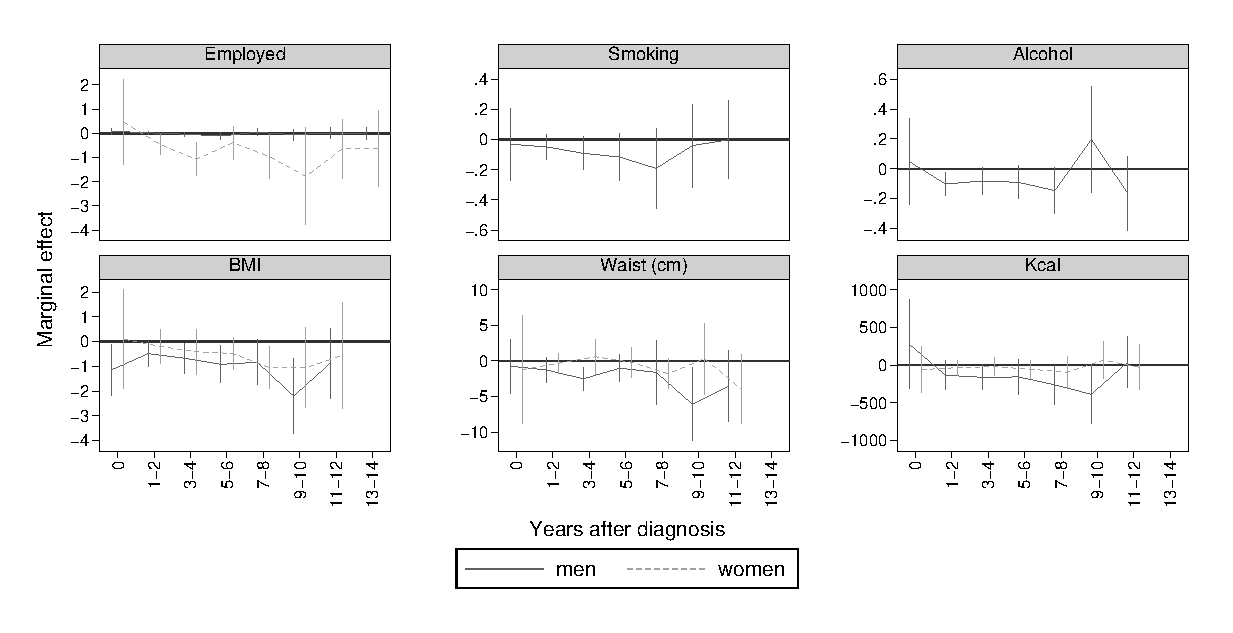
\includegraphics[width=\linewidth]{Chapter5/Figures/mi_msm_l_all.eps}
%DIFDELCMD < \end{center}
%DIFDELCMD < \end{figure}
%DIFDELCMD < \begin{figure}
%DIFDELCMD < \begin{center}
%DIFDELCMD < %%%
%DIFDELCMD < \caption{%
{%DIFAUXCMD
%DIFDELCMD < \label{fig:duration_g_fe_mi} %%%
\DIFdelFL{Analysis of the effect of time since diabetes diagnosis on employment status and behavioural outcomes (duration groups, fixed effects)}}
%DIFAUXCMD
%DIFDELCMD < 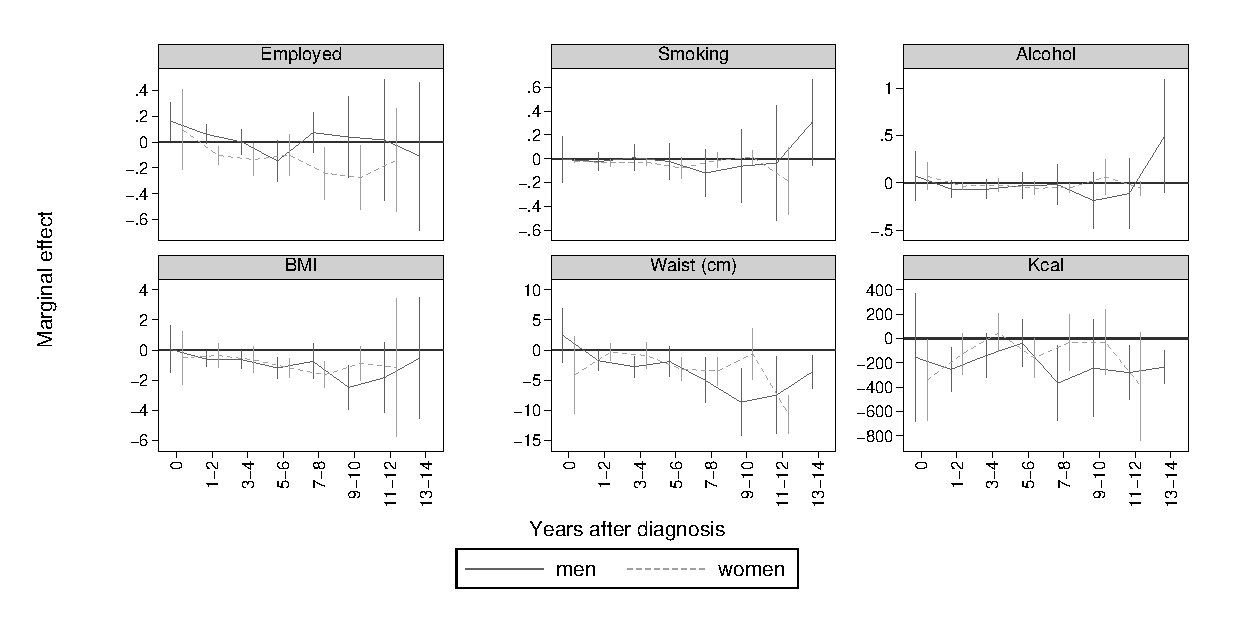
\includegraphics[width=\linewidth]{Chapter5/Figures/mi_fe.eps}
%DIFDELCMD < %%%
\DIFdelendFL \DIFaddbeginFL \DIFaddFL{\makebox[\linewidth]{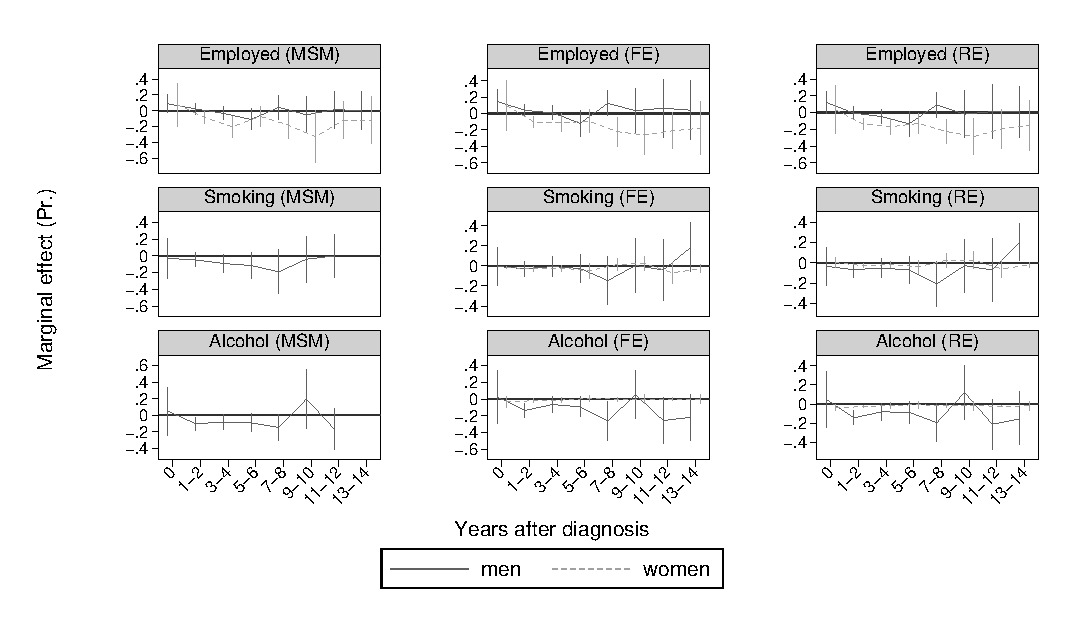
\includegraphics[width=\linewidth,height=\textheight]{Chapter5/Figures/binary.eps}}
}\DIFaddendFL \end{center}
\DIFaddbeginFL \footnotesize\textit{\DIFaddFL{Note}} \DIFaddFL{The visualized coefficients are based on the results of the regression models shown in Tables \ref{tab:duration_groups_msm} and \ref{tab:duration_groups_fe} in the appendix. 95}\% \DIFaddFL{confidence intervals.
}

\DIFaddendFL \end{figure}
\begin{figure}
\begin{center}
\caption{\DIFdelbeginFL %DIFDELCMD < \label{fig:duration_g_re_mi} %%%
\DIFdelendFL \DIFaddbeginFL \label{fig:duration_g_fe_mi} \DIFaddendFL The effect of time since diabetes diagnosis on \DIFdelbeginFL \DIFdelFL{employment status }\DIFdelendFL \DIFaddbeginFL \DIFaddFL{BMI, waist circumference }\DIFaddendFL and \DIFdelbeginFL \DIFdelFL{behavioural outcomes }\DIFdelendFL \DIFaddbeginFL \DIFaddFL{calorie consumption }\DIFaddendFL (duration groups\DIFdelbeginFL \DIFdelFL{, random effects}\DIFdelendFL )}
\DIFdelbeginFL %DIFDELCMD < 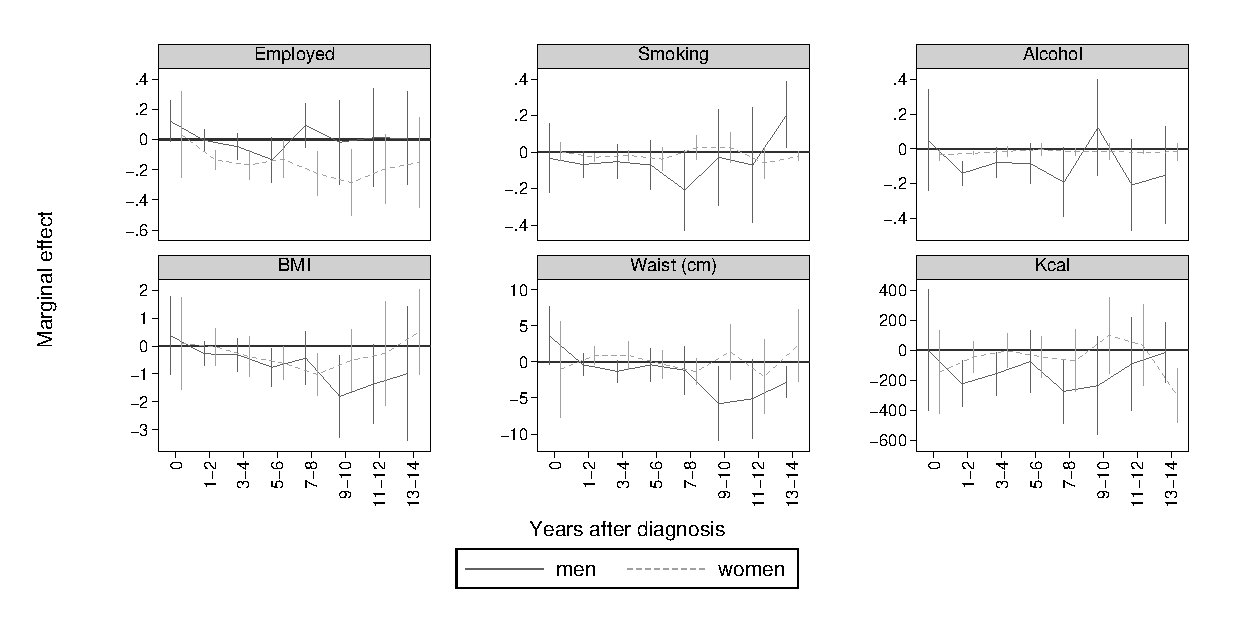
\includegraphics[width=\linewidth]{Chapter5/Figures/mi_re.eps}
%DIFDELCMD < %%%
\footnotetext{\textit{\DIFdelFL{Notes}} %DIFAUXCMD
\DIFdelFL{95}%DIFDELCMD < \% %%%
\DIFdelFL{confidence intervals}}
%DIFAUXCMD
\DIFdelendFL \DIFaddbeginFL \DIFaddFL{\makebox[\linewidth]{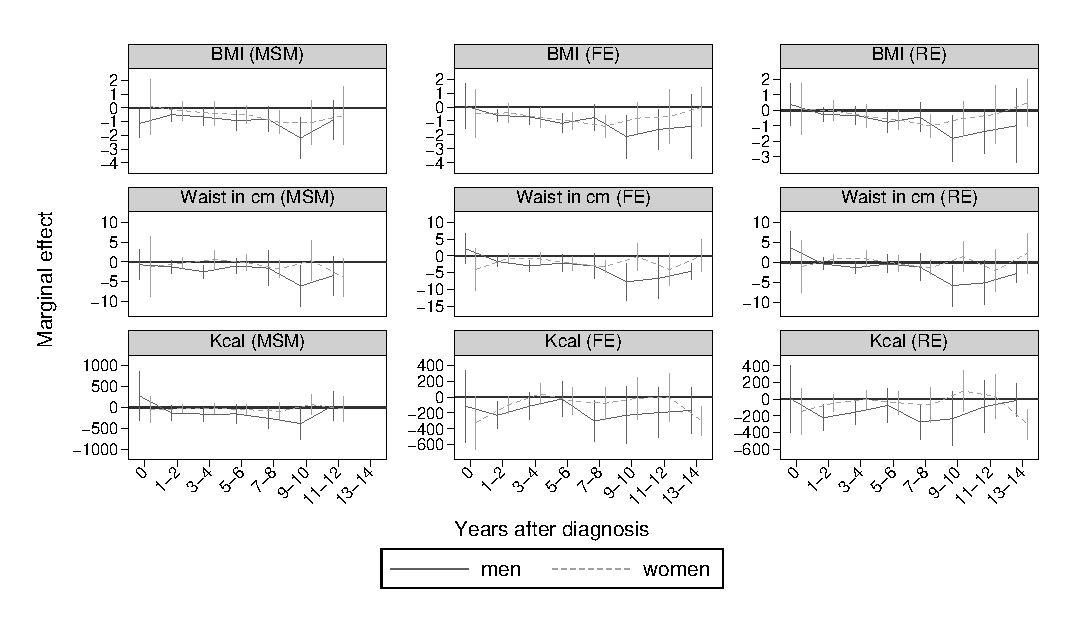
\includegraphics[width=\linewidth,height=\textheight]{Chapter5/Figures/continuous.eps}}
}\DIFaddendFL \end{center}
\DIFaddbeginFL \footnotesize\textit{\DIFaddFL{Note}} \DIFaddFL{The visualized coefficients are based on the results of the regression models shown in Tables \ref{tab:duration_groups_msm} and \ref{tab:duration_groups_fe} in the appendix. 95}\% \DIFaddFL{confidence intervals.
}

\DIFaddendFL \end{figure}
\end{landscape}


\section{\label{sec:Discussion5}Discussion}

The evidence for the impact of a diabetes diagnosis on employment probabilities and behavioural risk factors remains scarce, in particular in \acp{MIC}, where diabetes has become a mayor contributor to the burden of disease. We added to this evidence by exploring these relationships using longitudinal data from China, also improving upon previously used methodologies by taking into account the potential relationship over time between diabetes and these outcomes.

Our results suggest that receiving a diabetes diagnosis in China leads to a strong and lasting reduction in female, but not male, employment probabilities. We also found reductions in male \ac{BMI} and waist circumference, alcohol and calorie consumption and potentially smoking to be associated with a diabetes diagnosis. We did not, however, find similar changes in behavioural risk factors for women. Accordingly, it appears that women in China have to endure stronger adverse labour market effects of diabetes and at the same time are less successful then men at making risk behaviour changes to reduce their risk of diabetes complications.

The \ac{MSM} models and \ac{FE} models indicated very similar results suggesting that they are robust and that time-invariant confounding factors may play a limited role over and above baseline and time varying confounding factors. The \ac{MSM} results suggest that in particular \ac{BMI} and waist circumference levels as well as employment status can cause selection into a diabetes diagnosis and are then later themselves affected by the diagnosis, justifying the use of a \ac{MSM}. The \ac{RE} models further indicated that insufficiently accounting for confounding can---at least in this setting---lead to an overestimation of the impact of diabetes on employment status and an underestimation of the effects of a diagnosis on weight measures (\ac{BMI} and waist circumference). However, confounding may only be of limited relevance for  alcohol consumption, where the \ac{RE} models showed very similar results.

\subsection{Limitations}

The study has several limitations. While we used two estimation methods to reduce the influence of observed and unobserved confounding, respectively, none of the models is able to account for both forms of confounding. Therefore a causal interpretation is only possible under restrictive assumptions, namely no unobserved time-variant confounding for the \ac{FE} model and positivity, exchangeability and consistency for the \ac{MSM}. The assumption of positivity is likely to hold, given that every person should have at least a small chance of receiving a diabetes diagnosis. This is also supported by the relatively small range of stabilized weights and absence of zero-weights. The assumption of exchangeability or no unmeasured confounding could potentially be violated if not all time-invariant and time-variant confounders were accounted for, but this cannot be known for certain from existing data. We tested for part of this assumption by estimating a \ac{FE} model and, given that the results remained very similar, this suggests that unobserved time-invariant confounding may be of limited relevance in this case, even though this remains speculative as the Hausman test indicated some time-invariant confounding. Consistency would have been violated if a diabetes diagnosis had been reported but the person had actually not been diagnosed with diabetes. This was likely only violated in very rare cases of misreporting, given that specificity of diabetes self-report is very high in China \autocite{Yuan2015}. Because we were interested in the effect of a diabetes diagnosis, unobserved diabetes did not violate the consistency assumption.

A limitation of the \ac{FE} model is the possibility of time-variant confounding due to prior outcomes (for example employment status) affecting the current treatment (a diabetes diagnosis). We found some evidence that prior outcomes could affect selection into a diabetes diagnosis, potentially introducing bias in our \ac{FE} estimates. Given that the \ac{FE} estimates were close to those of the \acp{MSM}, it could be that this bias may not have been very strong. Overall, it remains difficult to pin down the potential source of a potential bias as, for example in the female employment models, both the \ac{MSM} and the \ac{FE} results are very similar while the \ac{RE} results indicate a somewhat bigger adverse effect. We have some evidence for both models that their underlying assumptions may not hold, with the Hausman test suggesting time-invariant confounding and the results of Table \ref{tab:predictors} indicating some time-variant confounding due to prior outcomes.

Finally, a limitation is that in this study we only observe the combined effect of all that entails a diabetes diagnosis.  However, a diabetes diagnosis can entail a variety of 'treatments' that are difficult to disentangle and may each have a distinct effect on the explored outcomes. 

\subsection{Potential mechanisms}

The effects of diabetes on employment and behaviour could work through several mechanisms. Firstly, the provision of information at diagnosis, may causes increases in stress and anxiety, but could also reduce anxiety by providing an explanation for the experienced symptoms \parencite{Peel2004}, with both potentially affecting productivity. Secondly, a diagnosis is also the starting point for medical treatment, which could help to alleviate symptoms and to lose weight, but also poses new challenges, in particular if treatment entails the exogenous provision of insulin or adherence to strict meal plans, likely adding to the burden of diabetes in daily life \parencite{vijan2005,Pibernik-Okanovic1996}. Thirdly, adherence to medical treatment may be heterogeneous across people with diabetes, with non-adherence likely leading to a further worsening of risk factors for complications, while good adherence may prevent or delay debilitating complications \parencite{Asche2011}. Fourthly, a diagnosis may also cause lifestyle changes such as increasing exercise levels, eating healthier and reducing smoking or alcohol consumption, all potentially affecting the risk of developing further complications and of changes in productivity. In the current study, it is not possible to ascertain the role of each of these factors in affecting employment probabilities and behavioural risk factors. Only for the reductions in smoking and alcohol consumption, it seems reasonable to attribute them to diagnosis induced awareness of the need to reduce these risk factors, as other pathways appear less likely to be relevant. 

The found adverse effect of diabetes on employment is in line with other studies on the labour market impact of diabetes that have found diabetes to reduce employment probabilities for women \parencite{Minor2011,Latif2009,Harris2009,Seuring2016}---often more than for men. Most comparable to our results are likely the results from Mexico in Chapter \ref{cha:Mex2}, which were also based on \ac{FE} estimations and data for a similar time period \parencite{Seuring2016}. The study found significant reductions for both males and females of about 5 percentage points. Taking into account the lower overall employment rate of Mexican women compared to men, this translated into a 16\% reduction in female employment probabilities, a figure comparable to the effect on Chinese women. However, in Mexico also men experienced adverse effects, unlike to what we found for China.

The found effects on changes in behavioural risk factors can be compared to the study by \textcite{Slade2012}. Slade finds reductions in alcohol consumption and smoking, though it appears that these reductions were not maintained over a longer time period. Unfortunately, Slade only provided information for the entire sample and the male sample, so that we cannot compare them directly with our results for women. In terms of the effect on weight, again both studies cannot be directly compared because Slade investigated the effect of a diagnosis on being overweight or obese, while we used continuous weight measures in our primary analysis due to the discussed difficulties of defining cut-off values for Asian populations. Slade found an initial reduction in weight status, but also that people with diabetes tended to become more likely to be overweight or obese after some time. Our results using overweight and obesity could tentatively be interpreted to indicate a more constant reduction in obesity over time, suggesting that reductions in weight in Chinese men may be longer lived than in the USA. Importantly---and in concordance with our findings---he found that simple covariate adjustment led to biased estimates of the impact on weight status, finding a positive relationship. This underlines the importance of accounting for potential sources of confounding.

The permanent reduction in male \ac{BMI} and waist circumference we have found has also been observed in a cohort of Danish patients \autocite{DeFineOlivarius2015}, where weight increased in the years preceding diagnosis, while after diagnosis weight decreased. The exact reasons for this decrease were unknown but attributed to motivation changes as a result of the diagnosis, concluding that the time around the diagnosis may represent a window of opportunity to obtain long lasting weight change. Nonetheless, reductions in weight may also be the result of treatment initiation with metformin or other diabetes drugs that have been shown to lead to weight reductions \autocite{Yang2014}. Importantly, the reduction in male \ac{BMI} levels and waist circumference were accompanied by reduced energy intake, suggesting that the changes in weight were at least partly the result of lower energy intake.  Further, given that in China diabetes incidence has been especially attributed to a high accumulation of visceral fat and central obesity \autocite{Ma2014}, the reductions in waist circumference may have had a particular positive effect on diabetes control and the prevention of comorbidities. Together, the lower levels of energy intake and waist circumference after the diagnosis allow for the interpretation that the reductions in \ac{BMI} were due to fat loss and not lower lean body mass \autocite{Klein2007}. 

For women, however, we did not find similar strong evidence for reductions in \ac{BMI}, waist circumference or energy intake. The relatively smaller effects for women could indicate a lower ability to change behaviours supportive of weight loss. This appears to be supported by the smaller reductions in energy intake. This could have---at least partly---contributed to a higher risk for diabetes complications further down the line, also adversely affecting employment probabilities. Apart from this, other explanations for the lower weight loss and larger employment penalty for women compared to men include their lower educational attainment, which has been indicated as a factor in preventing better glucose control \autocite{Luo2015} and may also affect the ability to successfully change behaviours. Lower income levels for females compared to men may also have negatively affected the ability to receive adequate treatment following a diagnosis, limiting their ability to change health behaviours \autocite{Luo2015}, increasing the risk of complications. We found that women with diabetes lived in households with lower income levels compared to men with diabetes, however, these income levels were still higher then for those without diabetes. Nonetheless, it may still be the case that women were less likely to access care due these differences in income. Moreover, there are likely biological factors that lead to worse health outcomes for women compared to men. There is some evidence that, due to different ways of fat storage between men and women, men tend to cross the diabetes threshold at an earlier point in time and at a comparatively healthier metabolic state then women \parencite{Peters2015,Peters2014a,Peters2014}. Women are more likely to have spend more time in a pre-diabetes state \parencite{Bertram2010} and to cross the threshold only once their metabolic health has significantly deteriorated, leading to a greater risk of cardiovascular disease and stroke \parencite{Peters2015}. Supporting this, a study for China found a greater prevalence of diabetes comorbidities in Chinese women compared to men \autocite{Liu2010}. In this light it may not be surprising that we find more conclusive evidence of worsening employment probabilities for women. If women are less likely to receive proper treatment and to change their health behaviours and at the same time have a greater risk for complications then men, the long term effects of diabetes on their health are likely more severe than for men and consequently affect their employment status to a greater extent.

Taken together, these estimation results suggest a lower risk of unemployment for men with diabetes potentially due to their greater ability to reduce behavioural risk factors, while the effect of diabetes on employment for women is substantial because no such changes in behaviour take place. Further analysis is needed to test this formally, and is beyond the scope of this paper.





\section{Conclusion}

Our results indicate worse outcomes for women then men after a diabetes diagnosis, with women experiencing a reduction in employment probabilities accompanied by and potentially partly due to an inability to reduce important risk factors for diabetes complications. For males, the opposite pattern is found, as they do not experience adverse employment effects and are able to achieve reductions in the investigated risk factors. These findings are robust to the application of two distinct, but complementary econometric techniques. Overall, given the large prevalence of undiagnosed diabetes, our results indicate that an early diagnosis may be a good way to foster early behaviour change that could lead to more positive health and economic outcomes for people with diabetes over time. It appears, however, that greater emphasis needs to be put on reducing the burden of diabetes for women to reduce the observed inequities in the impact of diabetes. Future research should try to unravel the mechanisms behind these differential outcomes for men and women, investigating more formally whether differences in behavioural risk factors could be a potential explanation.

\clearpage
 \newpage 
%\comment{
\acresetall  %resets all acronyms
\chapter{\label{cha:Discussion}Discussion and conclusions} 
\acresetall  %resets all acronyms
 \newpage \section{Chapter overview}
Diabetes has reached epidemic proportions in \acp{MIC} and is a major contributing factor to poor health and early mortality, as also discussed in Chapter \ref{cha:intro}. The economic impact of diabetes on individuals and healthcare systems has, however, received limited attention. In particular, we have a limited understanding of the effect of diabetes on individual labour market outcomes. Moreover, little is known about how people with diabetes currently achieve positive change in behaviour risk factors to prevent the disabling complications of diabetes, and whether this plays a role in the effect if the disease on labour market outcomes. The main goal of this thesis has been to assess the economic burden of diabetes in \acp{MIC}, focusing on two predominant and large countries with an increasing diabetes disease burden. This should help to better understand the importance of primary and secondary prevention of diabetes and to identify those populations \DIFdelbegin \DIFdel{must }\DIFdelend \DIFaddbegin \DIFadd{most }\DIFaddend susceptible to the adverse economic effects of diabetes.

Four separate studies were conducted that intended to answer the research questions posed in Chapter \ref{cha:intro}. This concluding chapter has four parts. Firstly, it summarises the principal findings. Secondly, it contextualises the findings within the wider literature and provides implications for policies. Thirdly it reflects on the methods. Finally, there are suggestions for future research and concluding comments.

\section{Summary of principal findings}



\paragraph{Chapter \ref{cha:review}} set out to provide an overview of and critically assess existing studies on the economic costs of type 2 diabetes globally. This not only included \ac{COI} studies but also studies on labour market outcomes. Systematic review methods were used and the evidence was synthesized narratively. 86 \ac{COI} studies and 23 labour market studies were identified. Of those, 24 came from \acp{LMIC}, with 23 being \ac{COI} studies.

For \ac{COI} studies, the review found a large range of estimated costs, with the largest per-capita costs \DIFdelbegin \DIFdel{being generated }\DIFdelend \DIFaddbegin \DIFadd{observed }\DIFaddend in the USA while costs were generally lower in \acp{LMIC}. However, in \acp{LMIC} treatment costs were paid almost entirely out-of-pocket by the poor due to a lack of health insurance coverage, consuming considerable parts of their annual income.  The review also found considerable differences in the methodologies used and in the study quality. This made it difficult to directly compare the results across studies. While in many \acp{HIC} studies an incremental costing approach was used and data sources were representative for a distinct population, studies in developing countries often had to rely on non-representative, relatively small convenience samples, often lacking a control group. Many studies also lacked explicit mentioning of the study perspective or of the costing components that were included. 

For labour market impact studies, most found adverse effects of self-reported diabetes on employment probabilities, wages or working days. Studies were concentrated on a few \ac{HIC}, in particular the USA. More recent studies took into account potential biases due to the endogeneity of diabetes, mainly using an \ac{IV} strategy with the family history of diabetes as an instrument. However, the direction of bias was ambiguous across different studies and countries. 

The review also identified methodological and thematic areas that previous research had only covered sparingly. No \ac{COI} studies took into account the possibility of biased estimates as a result of endogeneity of diabetes. Consequently, there is a lack of evidence in the literature about the potential bias in the cost estimates of diabetes \ac{COI} studies. Further, few studies used an incidence approach to investigate lifetime costs of people with diabetes, which could provide better information about the dynamics of cost increases post diabetes diagnosis. 

Despite these identified limitations of the \ac{COI} literature, the review provided a picture of the healthcare costs of diabetes in almost every continent. This was not the case for labour market studies, where almost no evidence was found for \acp{LMIC}. There is reason to expect the labour market impact of diabetes to be very different in \acp{LMIC} compared to \acp{HIC}, given the \acp{LMIC}' less advanced healthcare systems, later diagnosis but---in some populations---earlier onset of diabetes and greater susceptibility to develop it, the larger informal labour market and overall different labour market structure in \acp{LMIC}. Also, in terms of methodology, studies had not taken advantage of panel data techniques to get closer to a causal interpretation of their estimates. Especially studies on the effect on employment probabilities had instead relied on the same---at least debatable---identification strategy using \acp{IV}. Therefore, a study using a different identification strategy was warranted.

Importantly, no study investigating the impact of undiagnosed diabetes on labour market outcomes was identified by the review. Hence, an important part of the diabetes population had been mostly neglected. This left open the question in how far results for self-reported diabetes were applicable that part of the population that was unaware of their diabetes status.

Based on the findings of the review, the three research studies that followed addressed parts of the identified gaps, in particular focusing on labour market outcomes. 

\paragraph{Chapter \ref{cha:Mex1}} provided the first evidence for the impact of diabetes on employment probabilities in a developing country, where diabetes had become a public health concern. Because little was known about the equity impacts of diabetes, a further goal was to investigate the heterogeneity of effects across formal and informal employment and for the 'rich' and 'poor'. Due to the unavailability of an alternative identification strategy, the study applied the already established \ac{IV} approach using parental diabetes as the instrument. Using further background information on parental education, it improved upon earlier studies by controlling for a potential confounding pathway that could have invalidated the specific instrument. It further used two methods to implement the \ac{IV} approach. The main analysis was based on a bivariate probit model that had been shown to be better suited for our specific data, in comparison to a standard linear \ac{IV} model. We nonetheless also provided the results of the latter approach. Both models found no indication of diabetes being exogenous in this context so that a simple univariate probit model was used for inference. The results showed an adverse effect of diabetes on employment probabilities in Mexico, reducing them by about 10 percentage points for men and 5 percentage points for women. The subgroup analysis suggested that the adverse employment effects occurred mainly to those above age 44, while younger people seemed less affected. Also, being poorer increases the exposure to negative employment effects of diabetes. The same was the case for those in the informal compared to those in the formal labour market. Across all models, the point estimates were bigger for males than for females. 

\paragraph{Chapter \ref{cha:Mex2}}  went on to address several questions identified in Chapter \ref{cha:review} that had not been investigated in the first Mexico study. Further, the robustness of the findings of Chapter \ref{cha:Mex1} had to be tested using more extensive and recent data and a different identification strategy. Chapter \ref{cha:Mex2} thereby took advantage of a recent extension to the data used in Chapter \ref{cha:Mex1}. The data now spanned three waves and eight years, which allowed for the use of a longitudinal individual fixed effects model to estimate the relationship of self-reported diabetes with employment. Additionally, the investigated labour market outcomes were extended to wages and working hours. In addition, it was now possible to investigate the relationship of diabetes duration with labour market outcomes, in order to better understand the timing of any diabetes impact on labour market outcomes. Importantly, the additional wave also provided information on diabetes biomarkers to explore the effects of diabetes for the entire diabetes population as well as those unaware of diabetes separately.

The analysis carried out in Chapter \ref{cha:Mex2} confirmed the adverse relationship of self-reported diabetes with employment, finding a five percentage point reduction for males and females alike. Given the relatively low female employment rate, this translated into a 14\% relative decrease in employment probabilities for women compared to 6\% for men. Compared to the cross-sectional results of Chapter \ref{cha:Mex1}, the estimated effects of the \ac{FE} model are about half the size for men, but are similar and of stronger statistical significance for women. This is likely due to the additional data used in Chapter \ref{cha:Mex2}, but could also partly be the result of the different estimation technique. For wages and working hours no adverse effects of self-reported diabetes were found.

Further analysis showed that the most adverse effects were concentrated among self-employed and independent agricultural workers, potentially due to lower job security and access to healthcare in these often informal jobs. Further, Chapter \ref{cha:Mex2} revealed that the adverse effect of diabetes on employment appeared shortly after diagnosis, then levelled off for some time until it appeared again. This pattern was observed for both males and females, albeit only statistically significant for the former. Interestingly it was found that when the employment effects levelled off, wages started to fall, again for both genders. This suggested that during this period diabetes, plausibly through reductions in productivity, mainly reduced wages, without affecting job loss.

Finally, the results of the biomarker analysis presented in Chapter \ref{cha:Mex2} showed that relying on self-reported diabetes information can lead to measurement bias in the coefficient of diabetes. Using the biomarker data to identify people with diabetes, compared to self-reported diabetes smaller effects especially on employment probabilities were found. This was caused by the non-existent associations between undiagnosed diabetes and employment probabilities. It was further found, that part of the difference in effects between self-reported and undiagnosed diabetes could be explained by differences in subjective health status, with those self-reporting diabetes also reporting a worse health status. Interestingly, differences in \ac{HbA1c} levels did not drive the stronger effects for those self-reporting. %Add ttest to Chapter 4 showing difference in subjective health  


\paragraph{Chapter \ref{cha:China}} continued the investigation of the impact of self-reported diabetes on employment probabilities, but this time in China. It further investigated how a diabetes diagnosis affected diabetes-relevant health behaviours in a developing country. Because the relationships may be biased due to confounders not previously taken into account, the study used two different econometric strategies\DIFdelbegin \DIFdel{in }\DIFdelend \DIFaddbegin \DIFadd{: }\DIFaddend \acp{MSM} and \ac{FE}. Each controlled for a different source of confounding, improving the robustness of the identified effects. The dataset used consisted of six waves of the \ac{CHNS}, covering a period from 1997 to 2011.

The results from Chapter \ref{cha:China} provided further evidence of a deterioration of employment probabilities after a diabetes diagnosis, though this time only for women. They experienced a reduction in employment probabilities between 11 to 12 percentage points. For men, the \ac{MSM} and \ac{FE} models showed insignificant relationships. These reductions for women were similar to those found in Mexico (16--17\% in China and 14\% in Mexico) when the different female employment rates were taken into account. The results for behavioural risk factors also suggested different effects for men and women. According to the results, men were able to reduce alcohol consumption, \ac{BMI} levels, waist circumference and their daily calorie consumption, potentially reducing the risk for diabetes complications \parencite{Wilding2014}. For women, no strong evidence for similar reductions was found. A similar picture remained when investigating the effects over time using linear and non-linear specifications. On the one hand they suggested maintained reductions in female employment probabilities over time but no strong changes in risk factors. On the other hand, men were able to consistently reduce behavioural risk factors in the years following diagnosis while not experiencing any labour market penalties. Overall, the findings suggest a potential relationship of changes in risk factors with changes in labour market outcomes.

\section{Implications for policy making}

The findings of this thesis indicate an important global economic burden of diabetes and have added first evidence on the effect of diabetes on labour market outcomes in \acp{MIC}. The thesis also showed that diabetes---at least as far as labour market outcomes are concerned---did not similarly affect the population unaware of their diabetes diagnosis as it did those who were aware. Additionally it showed, that a diabetes diagnosis can elicit positive changes in behavioural risk factors, though to different degrees for men and women. Further, the distributional analysis brought to light that the burden of diabetes appears to be distributed unequally, disproportionally affecting the poor, those in the informal labour market and women.

These findings may lead to several implications to reduce the economic burden of diabetes in \acp{MIC}. 

\subsection{Inequities in the economic burden of diabetes}

An important finding of this thesis are the economic inequities in the burden of diabetes. In Chapter \ref{cha:review} the review found a high \ac{OOP} burden in \acp{LMIC}, especially for those with no insurance coverage. Chapter \ref{cha:Mex1} showed that the adverse employment effects were concentrated among those in the informal labour market and with fewer resources. This was further supported by findings from Chapter \ref{cha:Mex2} that indicated a greater reduction in employment probabilities to work in the agricultural or self-employed sector, while for those working in a non-independent wage job---that often entails greater contractual job security and better access to health insurance---diabetes did not appear to elicit negative effects. Chapter \ref{cha:China} found bigger adverse employment effects and more modestly positive behavioural changes in women compared to men after they had received a diabetes diagnosis. These gender inequities are also supported by the results for Mexico, in particular by Chapter \ref{cha:Mex2}, where, taking into account the lower overall employment rates for women in Mexico, the relative reduction in employment probabilities was much greater for females than for males.

There may be several potential strategies how to reduce these inequalities\DIFdelbegin \DIFdel{and improve access to care}\DIFdelend . In particular these include tackling the observed differences by gender, better prevention of diabetes, earlier diagnosis and better treatment of those diagnosed.

\subsubsection{Gender}

One of the main results of this thesis, is the identification of women with diabetes as a specific target group. Gender differences in the disease burden of diabetes have come to the forefront only recently \parencite{Peters2015}, but may hold one of the keys to reducing the economic burden of diabetes. However, it appears that biological differences between men and women may make it necessary to specifically target women \DIFdelbegin \DIFdel{. Diabetes likely affects them to a greater extent }\DIFdelend \DIFaddbegin \DIFadd{that are likely more affected by diabetes than men }\DIFaddend \parencite{Peters2015,Peters2014a,Peters2014,Bertram2010} \DIFdelbegin \DIFdel{and this }\DIFdelend \DIFaddbegin \DIFadd{which }\DIFaddend could be driving the observed differences in the economic effects. Efforts to reduce the burden for females would include increasing awareness among doctors about the higher risks for women to develop diabetes complications, as well as screening for cardiovascular risk factors in women at or before a diabetes diagnosis. This would present an opportunity to prevent a further escalation of the cardiovascular risk profile \parencite{Peters2015}. For women, weight reduction thereby seems to be the single most important step to reduce the risk of diabetes and ensuing complications \parencite{Peters2015}. As this thesis has shown, women in China were not able to achieve weight reduction to the extent men did and therefore may need to be treated differently. Future work on \acp{LMIC} can provide important contributions to help develop effective strategies to obtain this type of improvements in women's health outcomes.

Moreover, reductions in socioeconomic inequities identified in this thesis may also contribute to a reduction in the observed gender differences. If women have fewer economic resources than men, are more likely to work in the informal labour market and less likely to be insured \parencite{Galli2008} and therefore are more adversely affected by diabetes, then interventions targeting the poor and uninsured should specifically help women. Some of these interventions will be discussed below.

\subsubsection{Prevention}

Greater prevention of diabetes could help to reduce the observed inequities and the individual economic burden of diabetes. Given the inequities found in this thesis, such efforts may be particularly worthwhile if they focus on those disproportionally affected by the adverse economic effects of diabetes.

One option \DIFdelbegin \DIFdel{are }\DIFdelend \DIFaddbegin \DIFadd{is }\DIFaddend the introduction of national policies to affect food consumption. There is already some real life evidence of such interventions with the goal of reducing obesity in developing countries. In Mexico, a 10\% tax on purchases of sugar-sweetened beverages and 'junk food' has been introduced in 2014. First results suggested a reduction in purchases of these goods after the introduction of the tax, with a steeper decline for those with lower income levels \parencite{Colchero2016,Batis2016}. If these changes in consumption actually lead to a healthier diet and are large enough to cause reductions in obesity and diabetes prevalence has not been evaluated yet and remains to be seen. Other efforts to prevent diabetes in \acp{LMIC} include increasing the awareness of diabetes and how to prevent it via population level campaigns, and  increasing the accessibility to sport courses and fitness equipment to increase physical activity \parencite{Cefalu2016}. 

Another option is the identification of at risk groups and targeting them with interventions to increase physical activity and dietary changes. These have shown promising results across the globe, including in developing countries such as India and China, where interventions have caused long term reductions in the risk of developing diabetes \parencite{Cefalu2016}. For example, for China a randomized controlled trial provided long term lifestyle interventions to reduce the incidence of diabetes and cardiovascular disease as well as to reduce mortality in people at risk of developing type 2 diabetes. Over the active trial period of six years, the diet and exercise intervention reduced the relative risk for diabetes incidence by  over 50\% \parencite{Pan1997}. A more recent evaluation of the long-term impact of the interventions showed that over 20 years after the intervention had ended, the incidence of diabetes was still over 40\% lower in the intervention group. Further, people that had received the intervention spend 3.6 years less with diabetes than those in the control group \parencite{Li2008}. However, all these interventions were tested in randomized controlled trials, and translation into real-world settings in community-interventions has been less successful, even in high-income countries \parencite{Wareham2016, Kahn2014}. For example, weight loss has only been a small fraction of the reductions achieved in trials, often likely too little to prevent diabetes. \textcite{Kahn2014} argue that weight loss is notoriously difficult to maintain over a longer period of time, with trials often only capturing initial weight loss, but not the return to previous weight levels over time.  Therefore, prevention efforts based on lifestyle interventions or aiming at weight loss may not yet be translatable into real life, as too little is known about their cost-effectiveness and long-term effects to justify the use of limited resources \parencite{Kahn2014}. There are also questions about the cost-effectiveness of these interventions if scaled to a population level and the problem of finding qualified staff to implement lifestyle interventions at the local level. 

The evidence for pharmacological interventions mainly using metformin also indicates a reduction in the risk of diabetes. However, \textcite{Cefalu2016} mention the potentially large heterogeneity in the benefit of pharmacological interventions across ethnicities. More research on this subject will be needed to find out if successful pharmacological interventions in one ethnicity can be translated to other ethnicities. Nonetheless, \textcite{Cefalu2016} argue that preventive metformin treatment---which has been shown to reduce diabetes incidence in a number of randomized controlled trials---in individuals with a high risk of progressing to diabetes may be the best approach in countries with few economic resources. Low-cost generic versions of metformin exist, are considered essential diabetes medications in almost all \acp{LMIC} \parencite{Bazargani2014}, are effective in preventing or delaying the onset of diabetes, and are safe \parencite{Gomes2013}. They therefore may present a relatively cost-effective intervention that could be applied using existent healthcare infrastructure and pharmacies. It could be especially effective in \acp{MIC}, where the healthcare system infrastructure is much more developed than in \acp{LIC}. Nonetheless, specific targeting of populations most likely to benefit from pharmacological preventative treatment will be needed, as effects of metformin appear to be heterogeneous across age a diabetes risk. Further, pharmacological treatments may also exhibit different effects across populations and ethnicities \parencite{Cefalu2016}. 

The identification of high-risk individuals that could be targeted with the mentioned interventions may pose an additional hurdle to successfully preventing diabetes. Population level screening could be a way to identify people at risk. Screening could also be carried out at the workplace or the community and existing medical records could be used to identify people at an increased risk. Further, there may be possibilities to promote risk self-assessments using online resources through advertising and social media \parencite{Cefalu2016}. However, scientific evidence of the cost-effectiveness and feasibility of screening for high-risk individuals in \acp{LMIC} is non-existent, and if it where to happen may overwhelm health care systems. It also carries the risk of further widening health inequities if the lower income populations were less likely to attend screening efforts \parencite{Wareham2016}.


\subsubsection{Diagnosis}

If prevention is not successful and people have \DIFdelbegin \DIFdel{reached advanced to diabetes, }\DIFdelend \DIFaddbegin \DIFadd{developed diabetes, the }\DIFaddend earlier diagnosis of diabetes to prevent further complications could be a viable option to reduce the economic burden of diabetes. In Chapter \ref{cha:Mex2}, adverse labour market outcomes were only observed for the self-reporting diabetes population, suggesting that the adverse impact manifested only after some time of living with the disease and mainly after diagnosis. This is not surprising given the gradual increase in blood glucose as diabetes progresses and the concomitant relatively slow deterioration of health \parencite{Bertram2010}. While earlier detection of diabetes via screening did not yield important improvements in disease outcomes in the Addition-Trial in European \acp{HIC}, this might be markedly different in \acp{MIC}. The large undiagnosed population found in Mexico in Chapter \ref{cha:Mex2} as well as for other \acp{LMIC} in a recent study by \textcite{Beagley2014}, suggests that, compared to \acp{HIC}, in \acp{MIC} more people with diabetes remain undiagnosed for an extended period of time. Therefore, earlier detection may have a greater beneficial effect  \parencite{Choukem2013}, in particular if it can prevent complications from appearing within a person's productive lifespan. 
\DIFaddbegin 

\DIFaddend The results of Chapter \ref{cha:China} indicate that a diagnosis can introduce positive changes in behavioural risk-factors that may be directly related to a reduced economic burden of diabetes, suggesting that diagnosing those currently unaware could have positive effects. Nonetheless, earlier detection would also increase healthcare demands and costs, at least in the short term. Therefore evidence is needed that explores the trade-off between the costs generated by longer treatment periods and a greater number of patients due to an earlier diagnosis and potential reductions in healthcare expenditures and productivity losses as a result of lower complication rates at later stages \parencite{Engelgau2012}. Evidence on the cost-effectiveness of a population-based diabetes screening program was provided by a recent study from Brazil, where over 22 million people over the age of 40 were screened for diabetes, being the first evaluating an actual real-life population-based diabetes screening program in a developing country \parencite{Toscano2015}. It was unclear if the program could be considered good value for the healthcare system, as the cost-effectiveness of the findings depended strongly on the assumptions used about how effective treatment would be in preventing coronary heart disease and stroke. Given the results from this thesis, cost-effectiveness might be greater from a societal perspective if an earlier diagnosis would prevent or decrease losses in productivity and productive lifespan. Of course, early diagnosis may only be reasonable if the healthcare system is sufficiently developed to allow all diagnosed cases access to appropriate treatment options \parencite{Toscano2015,Engelgau2012}. 

Apart from worse health in the population aware of its diabetes, another policy relevant reason for the difference in the observed effects could be the psychological effect of a diabetes diagnosis. Reductions in productivity may be the result of increasing anxiety and depression as a result of becoming aware of the disease and its potential consequences. Further, difficulties in adapting to the treatment regime may cause additional stress. As discussed in Chapter \ref{cha:Mex2}, there is some evidence that becoming aware of the disease leads to reductions in labour income likely due to its psychological effects \parencite{Liu2014}. If this is confirmed by other studies, then strategies to provide better guidance and support at diagnosis and thereafter to reduce the psychological burden of the disease could be worthwhile.



\subsubsection{Treatment}

Earlier diagnosis, however, will only be worthwhile if those diagnosed are able to receive effective diabetes treatment. The adverse labour market effects found for those with self-reported diabetes and the increase in effect size over time after diagnosis, suggest that currently this may not be the case and adverse health and ensuing economic events often cannot be prevented. This may have several reasons. The diagnosis could happen too late to prevent first complications from having developed, making it increasingly difficult to prevent further complications. Another reason could be the sub-optimal treatment of the disease, in particular in the most adversely affected---likely socioeconomically disadvantaged---groups identified in this thesis.

Therefore, an important step to improve outcomes would be the provision of better quality in diabetes treatment, targeting the identified groups and tailoring interventions according to their socioeconomic, physical and personal characteristics \parencite{Cefalu2016}. The existing evidence on diabetes treatment models applicable in very resource constrained settings has recently been reviewed by \textcite{Esterson2014}. While the evidence is still limited, the study provided information on interventions that have had some success in improving diabetes treatment for the poor. Further, it identified common characteristics of these successful interventions: collaboration, education, standardization of guidelines and algorithms, technological innovations, and resource optimization. The authors recommended that initiatives to provide care to underserved populations should be built on collaborations between academic institutions, hospitals, the private sector and other organizations such as local governments. This should help to achieve goals that would otherwise be difficult to reach for one stakeholder alone. Further, programs should aim at providing appropriate education to doctors to increase their ability to successfully treat people with diabetes. For very remote communities \textcite{Esterson2014} suggested the use of peer-support programs, so that few well educated community members or nurses could help their peers with the challenges of diabetes management. Further, a need for standardized guidelines and treatment algorithms was identified as a means for healthcare professionals to improve and maintain their standards of care. Given that mobile phones have already reached even very remote areas and are common in the developing world, interventions based on existent technologies could also improve care and diabetes outcomes. They could facilitate communication between doctors and their patients as well as tracking and controlling diabetes management and outcome measures. Finally, resource optimization to use available and constrained resources more effectively, e.g., by transferring certain responsibilities from doctors to nurses or from healthcare professionals to peers could be an option in very resource constrained settings \parencite{Esterson2014}. Together, the presented strategies could help in reaching and treating poorer parts of the population.

A number of \DIFdelbegin \DIFdel{relevant }\DIFdelend interventions have been implemented in \acp{LMIC} to improve care for people with diabetes\DIFdelbegin \DIFdel{, causing improvements in risk factors}\DIFdelend . Focusing on China, Mexico and other \acp{MIC}, some of these will be mentioned here. Most of these interventions apply at least one of the recommendations mentioned in the previous paragraph. For Mexico, a recent randomized controlled trial tested the effects of providing better diabetes training to physicians as well as supporting them with nurses trained in diabetes care and peer-support groups \parencite{Contreras2016}. \DIFdelbegin \DIFdel{In a separate treatment}\DIFdelend \DIFaddbegin \DIFadd{Further}\DIFaddend , the additional monitoring and support of patients via the use of mobile phone technology was tested in a second intervention group, given the common use of mobile phones in Mexico. First results indicated a significant reduction in \ac{HbA1c} and better diabetes knowledge in both intervention groups compared to standard care, with better, but not statistically significant outcomes, for the group also using mobile phone technology. Other studies investigating the use of mobile phone technology have also shown promising results \parencite{Singh2016}. Two randomized controlled trials investigated ways to improve diabetes outcomes in Costa Rica and China, respectively \parencite{Goldhaber-Fiebert2003a,Sun2008}. In Costa Rica, the application of a community-based nutrition and exercise program led to reductions on weight, fasting glucose and \ac{HbA1c} levels. In Shanghai, China, more extensive diabetes education and the provision of meal plans led to improvements in blood glucose, \ac{HbA1c} levels, blood pressure and waist-to-hip ratios compared to the group receiving standard diabetes eduction.  Unfortunately, so far information about the ultimate value of these interventions in terms of their cost-effectiveness and long term effects is scarce, partly because the investigation is still under way \parencite{Contreras2016} or has not (yet) been evaluated \parencite{Singh2016}.

Further, in \acp{MIC}, the provision of universal health care has been advocated as a means to reduce health inequities by providing everyone with the ability to access healthcare \parencite{Marmot2008}.  Mexico has been one of the countries where the goal of universal health care has been almost accomplished through the introduction of ``Seguro Popular'', which provides those without prior health insurance coverage with social security and access to diabetes treatment options \parencite{Knaul2012,Rivera-Hernandez2016}. However, evidence on the impact of diabetes treatment and outcomes has shown that the availability of this program has only led to very modest improvements, only finding a positive effect on the use of pharmacological therapy. No effects were found on the monitoring of blood glucose or adherence to exercise plans by people with diabetes \parencite{Rivera-Hernandez2016}. A likely reason for this brought up by the authors was that many clinics were not prepared to provide specialized diabetes care and medications, suggesting that barriers to accessing appropriate diabetes care and education still existed. Hence, while public health care provision for those previously uninsured can reduce inequities, such programs need to ensure that their efforts are not sabotaged by the low quality of the offered services.


\DIFaddbegin \subsubsection{\DIFadd{Communicable diseases and structural constraints}}

\DIFadd{The mentioned strategies may be able to reduce the diabetes, however, they mostly focus on diabetes only and do not take into account potential possibilities for the integration of treatment with other diseases common among the poor, nor do these interventions address overall structural problems responsible for the inequities in the burden of diabetes. They therefore tend to represent temporal solutions aiming to address specific needs of people at risk of or living with diabetes under current circumstances, but may not help to substantially reduce the burden of diabetes in the long term if structural constraints existent in most }\acp{MIC} \DIFadd{are not taken into account. 
}

\DIFadd{A first constraint to the successful implementation of above mentioned interventions is the wider disease burden, which may inhibit the healthcare system  from providing effective treatment for diabetes and other chronic diseases. However, integrating diabetes care with the healthcare for other diseases may also present a viable opportunity for healthcare systems in }\acp{MIC}\DIFadd{.
}

\DIFadd{Health systems in developing countries have been slow to adopt technologies to reduce the burden of communicable diseases, maternal and perinatal conditions as well as nutritional deficiencies }\parencite{Gutierrez-delgado2009}\DIFadd{. The main reasons for this slow adoption are social and political instability limiting long-term planning, a lack of resources to finance the introduction of health technologies, and a dearth of qualified personnel in the public sector due to a lack of training and the loss of qualified personal to the private sector or health systems in developed countries }\parencite{Gutierrez-delgado2009}\DIFadd{. Therefore many }\acp{MIC} \DIFadd{face a double disease burden with high rates of communicable and non-communicable diseases at  the same time }\parencite{Gutierrez-delgado2009}\DIFadd{. The treatment of }\acp{NCD} \DIFadd{places additional pressure on health systems that did mainly developed to provide acute care of infectious diseases based on single-visit treatments and are lacking the infrastructure, resources and experience for the treatment of chronic diseases such as diabetes }\parencite{Nulu2016}\DIFadd{. Policy makers in }\acp{MIC} \DIFadd{therefore are forced to make decisions about the prioritization of treatments in an effort to use the available resources in a cost-effective as well as equitable manner }\parencite{Gutierrez-delgado2009}\DIFadd{, potentially limiting a systems ability to provide effective diabetes care.
}

\DIFadd{To improve treatment for diabetes under these circumstances, a greater integration of health services and control efforts of diabetes with the treatment of communicable diseases could help to exploit synergies and interactions between diabetes and communicable diseases. One such example presents the known relationship of diabetes with tuberculosis, where diabetes patients have a two- to threefold higher risk to develop tuberculosis. Further, tuberculosis may also complicate glucose management in people with diabetes }\parencite{Dooley2009}\DIFadd{. Therefore, instead of competing for resources, the detection and treatment of both diseases may be integrated to reduce costs and improve health outcomes }\parencite{Marais2013}\DIFadd{. Because tuberculosis and other communicable diseases are more common in groups of lower socioeconomic status with less access high quality care, the double burden with diabetes and the interplay between the diseases has the potential to even further increase the already existing health and social inequities }\parencite{Marais2013}\DIFadd{.  Therefore, focusing on ways to take advantage of the synergies presenting themselves in the treatment of communicable and non-communicable diseases could provide a way to reduce the overall disease burden, in particular of more marginalized populations, which could also reduce the existing inequities while limiting the strain on healthcare budgets.
}

\DIFadd{Additionally, studies have consistently shown a relationship of early life health with later life health outcomes, suggesting that bad health and nutritional status early in life could increase the risk to develop diabetes and other diseases later  }\parencite{Currie2013,Hanson2012}\DIFadd{. Therefore, efforts to improve maternal and early life health outcomes of children will not only have short-term effects but likely help to prevent adverse health outcomes later in life }\parencite{Marais2013,Bygbjerg2012}\DIFadd{. As a result, investing in the treatment of infectious diseases, nutritional deficiencies and maternal health could help to reduce the overall disease burden now and in the future. Further, because again it is the poor that are likely most exposed to the risk of adverse early life events, such efforts would likely help to reduce the economic inequities found in this thesis.  
}

\DIFadd{However, while a grater integration of diabetes care with the care of other diseases may be a viable way forward, these changes in the formal health-care sectors will not be sufficient. Because of the feedback loops between poverty and bad health, i.e. poor people are more likely to be sick which then further worsens their economic situation, socioeconomic inequities themselves are drivers of the disease burden }\parencite{DiCesare2013}\DIFadd{. Consequently, structural problems such as an unequal distribution of power, financial resources, education, the environment, housing as well as access to high quality health care,  need to be addressed. Only this will help to achieve lasting reductions in inequalities and consequently also the disease burden due to both communicable and non-communicable diseases }\parencite{DiCesare2013}\DIFadd{.
}

\subsubsection{\DIFadd{Discrimination of people with diabetes}}

\DIFadd{Despite the proposed efforts to reduce inequities in the burden of diabetes, people with diabetes may still face discrimination. The thesis has found considerable adverse effects of diabetes on employment chances which may not only be explained by its health impact, but also by employers discriminating against people with the disease. Once employers are aware of the employee's diabetes, they may decide to replace the employee with a healthy person as they suspect reductions in productivity due to health problems or disease management at the workplace. Little information exists regarding the importance of discrimination of employers against people with diabetes in }\acp{LMIC}\DIFadd{. For the USA, studies show that people with diabetes were more likely to experience discharge, constructive discharge or suspensions affecting their ability to retain their job }\parencite{McMahon2005}\DIFadd{. Further, working for smaller employers, being older and the ethnic background affected the risk of experiencing discrimination due to diabetes in the workplace. Similarly, a study for Switzerland found that people with diabetes were less likely to be hired and diabetes related events---such as hypoglycemia---made it more likely to experience job loss }\parencite{Nebiker-Pedrotti2009}\DIFadd{. Even though we have no information about the importance of discrimination for the employment effects found in this thesis, given the evidence from }\acp{HIC} \DIFadd{it is likely that it plays a considerable role. The adverse effects for the poor and informally employed found in this thesis suggest that discrimination may play a more important role in manual occupations that value physical health to a greater extent than more brain based jobs in the formal sector. Additionally, informal jobs are not affected by job security legislation }\parencite{Ulyssea2010,Loayza2011}\DIFadd{, reducing the costs of hiring and training a new employee, making it easier to replace a 'unhealthy' with a 'healthy' employee, further incentivising discrimination against people with diabetes.
}

\DIFadd{Unfortunately, simple remedies for this type of discrimination are difficult in }\acp{MIC}\DIFadd{. Because informal labour markets are a substantial part of transition economies, legislative measures to reduce the incentives of discriminating against people with diabetes may fall short---at least partly---as they would not be enforceable in the informal sector. Further, stricter protection legislation may have counterproductive effects in middle-income countries if they lead to reduced hirings of people with diabetes or those at a higher risk to develop diabetes, such as overweight or obese candidates }\parencite{Muravyev2014}\DIFadd{. Companies may be inclined to demand health check-ups prior to hiring to prevent the employment of personal with a higher risk of adverse health outcomes. Therefore measures to reduce discriminatory behaviour in employers in }\acp{MIC} \DIFadd{should also aim at reducing prejudices about people with diabetes, increase the knowledge about the treatment of the condition and the potential to prevent its adverse health consequences.
}


\DIFaddend Overall it seems that for \DIFdelbegin %DIFDELCMD < \acp{LMIC}%%%
\DIFdelend \DIFaddbegin \acp{MIC}\DIFaddend , national policies to change food consumption behaviours to prevent diabetes \DIFdelbegin \DIFdel{are currently }\DIFdelend \DIFaddbegin \DIFadd{could currently be }\DIFaddend the best option to halt the escalation of the economic impact of diabetes and to reduce inequities. The results of this thesis suggest that it should be a priority to design interventions that address the existent inequities by preventing diabetes in those populations that experience the worst economic consequences\DIFdelbegin \DIFdel{. Further, targeting those with little access to healthcare in screening programs for both undiagnosed diabetes and those at high-risk for diabetes, and then following up with offers for preventive }\DIFdelend \DIFaddbegin \DIFadd{, i.e. the poor and more marginalised groups of a country. One way to reduce the existing inequities using the existing health care system would be the integration of the treatment of diabetes with already existing strategies to treat related communicable diseases, common among underserved populations. This would also reduce competition for resources to treat different diseases, a problem facing many decision makers in very resource constrained healthcare systems. The evidence base for the effectiveness of screening programs, preventative }\DIFaddend pharmacological treatment and \DIFdelbegin \DIFdel{potentially also lifestyle interventions could be of value, but more conclusiveevidence on their cost-effectiveness and sustainability will be needed first. Further, strategies to improve treatment of diabetes }\DIFdelend \DIFaddbegin \DIFadd{lifestyle interventions is less conclusive, potentially due to the social and economic structural constraints existent in many }\acp{MIC}\DIFadd{, preventing their successful implementation. Therefore, the structural problems underlying the already existing social, economic as well as health inequities }\DIFaddend will need to \DIFdelbegin \DIFdel{take into account the specific circumstances of the respective target group and should be developed in cooperative efforts to make them work}\DIFdelend \DIFaddbegin \DIFadd{be addressed to achieve long term reductions in the burden of diabetes. This also pertains to issues of discrimination of people with diabetes at the workplace, currently being mostly unprotected from such behaviour due to the large informal labour markets in }\acp{MIC}\DIFaddend .



\section{Strengths and limitations}

The strengths and limitations of each study and the methodological approach used have been evaluated within each chapter. Additionally, the thesis overall has strengths and limitations.


A strength of this thesis is the provision of a comprehensive overview and assessment of the state of economic research on the impact of diabetes. It provides other researchers guidance by identifying areas for future research and suggestions on which methods to use. Further, the thesis itself fills some of the identified gaps by investigating the impact of diabetes on labour market outcomes in \acp{MIC}. A strength of these analyses is the use of rigorous econometric approaches taking advantage of available and previously underexplored, high quality, household data, allowing to investigate a variety of topics in the absence of experimental data. One of the challenges was the choice of the most appropriate method to establish a causal relationship. The main concern was that unobserved variables, measurement error as well as reverse causality may introduce bias into the estimates. A variety of methods were used that each had advantages and disadvantages in terms of the underlying assumptions and the ability to account for potential sources of bias. Their choice was mainly guided by the available data and the best way of achieving a causal interpretation under the given circumstances. Nonetheless, regardless of the method used, results consistently showed an adverse relationship of self-reported diabetes with employment probabilities, suggesting a relatively robust and likely causal effect. The methods used also improved upon previous approaches, providing more robust evidence and also incorporated methods predominantly known in epidemiology. 

A further strength is the provision of evidence on the potential of diabetes to widen the economic inequities in developing countries, identifying the groups that were disproportionally affected by the disease. Further, it has also advanced the understanding of diabetes as a multifaceted condition by exploring effects over time and for those who are aware and those who are unaware of their diabetes. Finally, it provides evidence from different data sources and contexts and also investigates the value of becoming aware of the disease through a diagnosis and its ability to influence health behaviours.

The thesis has several limitations. Whilst the intention was to provide evidence on the economics of diabetes in \acp{MIC}, the thesis mostly investigates the economic impact of diabetes. While this provided important information for researchers and policy makers, the thesis did not investigate how to curb this economic diabetes burden. Information about the best and most costs-effective interventions that could be applied in \acp{MIC} to lower the burden of diabetes is urgently needed as information about who is affected most will not suffice to effectively reduce the burden. Research on how to implement interventions feasible in non-\ac{HIC} settings is therefore of paramount importance, but was beyond the scope of this thesis.

This leads to the next limitation. The thesis does not investigate in how far healthcare systems in \acp{MIC} need to change in order to better provide care. Because they often lack financial resources, do not efficiently use the available resources, are designed to treat acute infectious diseases rather then affecting the outcomes of long-lasting non-acute \acp{NCD}, and often provide unequal access to their health services due to financial constraints of those seeking care, research into how to better equip healthcare systems to confront the challenges of treating \acp{NCD} is urgently needed \parencite{Mills2014,Guzman2010}.

A further limitation is the geographical concentration of the thesis, as far as the empirical, analytical chapters are concerned. While Mexico and China are among the ten countries worldwide regarding the absolute size of their diabetes population, there are other large and small \acp{MIC} currently facing similar challenges \parencite{Risk2016}.  It cannot be assumed that the evidence provided in this thesis is perfectly representative of all other \acp{MIC}. There is hence a need to investigate the economic burden and potential solutions in other countries, given their own specific context in terms of culture, the political system, economic development and existing inequities.

Finally, while the thesis intended to provide a picture of the potential inequities in the economic impact of diabetes for socioeconomic subgroups, it did not investigate in detail why these inequities exist and could only speculate on the reasons. A better understanding of the underlying reasons will be essential for designing adequate strategies to address these inequities. Further, whilst the thesis has touched upon the potential reasons for the differences in employment effects between those self-reporting diabetes and those unaware, it has not provided an in depth analysis of this phenomenon. A better identification of the underlying reasons will be required to design interventions that can prevent the adverse economic effects of diabetes. 



\section{Suggestions for future research}

This thesis has shown the global economic impact of diabetes and its adverse effect on labour market outcomes in Mexico and China. It identified the poor, those in the informal economy and women as being most adversely affected by the disease. It further found that, at least in China, it is men that appear to make the most from a diabetes diagnosis in terms of positively changing their health behaviours. Finally, it provided some indication that while self-reported diabetes is related to adverse labour market effects, undiagnosed diabetes is not. Without a greater understanding of the underlying reasons for the differences found, it will be difficult to design policies that can help prevent the burden of diabetes in \ac{MIC} and reduce inequalities.

Several reasons for the observed gender differences in the impact of diabetes have been discussed in this thesis, including biological reasons that increase the risk of complications in women \parencite{Peters2014,Peters2015,Arnetz2014,Roche2013,Policardo2014,Catalan2015,Engelmann2016,Seghieri2015} and may also impair the ability of women to lose weight \parencite{Penno2013}, as well as differences in the access to appropriate healthcare \parencite{Penno2013}. One strategy to further investigate these differences would be the use of biomarker data in combination with information on healthcare utilization as well as socioeconomic outcomes. This could then be used to investigate potential heterogeneities in the relationship between diabetes and overall metabolic health with labour market outcomes. Further, information on healthcare usage could be used to investigate if differences in healthcare access mediate the economic impact of diabetes. A potentially rich source of information is provided by two Chinese household surveys, the \acf{CHNS} and the \acf{CHARLS}. Both contain an extensive list of measured biomarkers and socioeconomic variables that could help to investigate gender differences in metabolic risk. Because biomarker data were only available for one wave in both the \ac{CHNS} and \ac{CHARLS}, in the present studies they could not be used longitudinally to predict future effects of diabetes. However, they will be able to be used for this purpose in future waves. This information may also be used to further explore differences in metabolic risk between people aware and unaware of their diabetes. Also, studies measuring potential mediating variables---such as knowledge, motivation, treatment, diabetes control and complications---would help clarify the causal mechanisms through which diabetes affects economic and other outcomes. Structural equation and mediation models could be useful with such data. 

Researchers should also try to confirm the results regarding the inequities found, using different data and countries. Whether these relationships can be confirmed or not, the underlying drivers of these inequities need to be explored to design adequate policies. This could be done by identifying countries where these inequities may not have been found, to isolate the causal determinants. Further, strategies implemented currently or in the future in \acp{MIC} that aim at reducing these inequities, such as the implementation of universal health insurance schemes need to be evaluated in how far they are actually achieving this goal in terms of diabetes. The same is true for population level interventions such as taxes on foods or nutrients, as these are probably regressive and theoretically should reduce consumption in particular for those with lower levels of income \parencite{Mytton2012c}. This could then lead to a reduction in diabetes incidence in these groups. However, depending on the price elasticities of the taxed products, such taxes may only reduce the disposable income of the poor, leading to reductions in the consumption of other, potentially healthier foods. They therefore may be seen as taxes on the poor, raising political and ethical dilemmas. Further, substitution effects with equally untaxed products may only cause a shift in consumption towards other equally unhealthy, but untaxed products \parencite{Mytton2012c}.

The diabetes population in all countries, but especially in \acp{LMIC} is only partially observed. In other words many people with diabetes are not aware that they have the disease. This thesis has provided an investigation of the differences between those who are aware and unaware in Chapter \ref{cha:Mex2}. It, however, still remains unclear to what extent different factors such as health information and actual health status are causing the observed heterogeneity in the economic impact. Because increasingly household surveys are providing biomarker data in combination with socioeconomic information, they should be used together with quasi-experimental econometric techniques to investigate this topic. A regression-discontinuity design may be used in a similar vein as in \textcite{Zhao2013a}, who use cut-off values for hypertension to identify those newly diagnosed and the subsequent effect of this diagnosis on health behaviours. A similar approach could be used to explore the effects of a diabetes diagnosis and the entailed health information on labour market outcomes, health behaviours and other economic outcomes. Importantly, research should assess the heterogeneity of effects across income groups, rural versus urban, education levels and between males and females. This would provide important information for designing interventions to reduce the physiological and economic burden of diabetes while preventing a widening of inequities.

Finally, there is a need to explore further economic downstream effects of the economic impact of diabetes. If diabetes causes reductions in employment and potentially also income, it is likely that these will cause not only problems for the individual directly affected, but for the entire household as well. In \acp{MIC}, where social security is less extensive and comprehensive, adverse health shocks due to diabetes could have consequences for the children, spouses or other family members living in affected households \parencite{Alam2014}. The loss in labour income due to diabetes needs to be compensated either by increasing the labour supply of other household members or by reducing expenditures for other consumption goods. Both could affect children directly, for example by reducing the time for or quality of education when tuition fees cannot be paid anymore and also by having to substitute time for education with labour time. Similarly spouses may be forced to increase their labour supply, reducing the time they can care for their children. These effects have remained unexplored for diabetes but given the scale of the diabetes epidemic may not be trivial.



\section{Conclusion}

Diabetes presents a major challenge for \acp{MIC}, but evidence on its economic effects has been scarce. This thesis has found that diabetes has an adverse economic impact on individuals and puts a burden on healthcare systems. Because evidence on the impact of diabetes on labour market outcomes was lacking in developing countries, the thesis did focus particularly on this topic. Thereby it not only provided evidence of the adverse impact of diabetes on employment, but also improved upon previously used econometric methods by using novel strategies to identify a causal relationship. The thesis also identified potential inequities in the impact of diabetes, pointing to larger adverse effects for the poor, those in the informal labour market and women. But the thesis did not only focus on the economic impact of diabetes, but also investigated the effects of a diabetes diagnosis on health behaviours, unravelling evidence for differences in the ability to change health behaviours between men and women.

These findings suggest that there is a need to reduce the economic impact of diabetes in \acp{MIC}. Considering the increasingly earlier onset of diabetes and the ongoing increase in incidence in many countries, the non-trivial adverse economic effects could otherwise hinder economic development and present a substantial poverty risk. Strategies to combat the adverse diabetes effects need to be tailored to the available resources within countries, target the most affected groups to narrow inequities, also having in mind potential gender differences. Finally, there is a large undiagnosed diabetes population in \acp{MIC} that is likely to experience severe diabetes complications if identified very late. Hence, ways to diagnose this population earlier in order to prevent further deterioration of health may go a long way in preventing and delaying the most catastrophic economic and health outcomes.

In conclusion, it is hoped that the research presented in this thesis contributes to the knowledge on the economics of diabetes and help to identify cost-effective strategies to lower the health and economic consequences of diabetes. It has demonstrated the economic burden currently caused by diabetes, in particular in Mexico and China, and has identified groups that are particularly vulnerable to the negative consequences of the disease and should be at the centre of efforts to prevent the burden of diabetes. \newpage 
\printbibliography[heading=bibintoc]
\chapter*{\label{cha:Appendix}Appendices}
\addcontentsline{toc}{chapter}{\nameref{cha:Appendix}}
\renewcommand{\thechapter}{{\Roman{chapter}}} 
\renewcommand{\thetable}{A\arabic{table}} %changes chapter number to roman
\renewcommand{\thefigure}{A\arabic{figure}} %changes chapter number to roman
\setcounter{chapter}{0}  % sets chapter counter to zero to start numbering again for appendices with roman numbering
\setcounter{table}{0}
\setcounter{figure}{0}
 \newpage 

\chapter{Appendix to Chapter \ref{cha:intro}}

\begin{landscape}
\footnotesize{
\begin{tabularx}{\linewidth}{XXXXXXXXXXXXXX}
\caption{\label{tab:datasets}Household surveys from low- and middle-income  countries including diabetes information as of 2014} \\
\toprule
Name & Country & Cross-section / Panel & Waves & Years & Population & Sample size & Nationally Representative & Ongoing & Data available & Interesting content & URL \\  \midrule \endfirsthead %second time to prevent caption at each additional page
\caption[]{Household surveys from low- and middle-income  countries including diabetes information as of 2014} \\
\toprule
Name & Country & Cross-section / Panel & Waves & Years & Population & Sample size & Nationally Representative & Ongoing & Data available & Interesting content & URL \\  \midrule \endhead
DHS & Armenia & Cross-section &  & 2010 & women and men 15-49 & 6700 households & yes & no & yes & diabetes questions, health expenditures &  \url{http://www.measuredhs.com/what-we-do/survey/survey-display-354.cfm} \\
DHS & Bangladesh & Cross-section &  & 2011 & women 12-49 and men 15-54 & 17141 households & yes & no & yes & & \url{http://www.measuredhs.com/what-we-do/survey/survey-display-349.cfm} \\
DHS & Benin & Cross-section &  & 2011-2012 & women 12-49 and men 15-64 & 17422 households & yes & yes & not yet & diabetes questions & \url{http://www.measuredhs.com/what-we-do/survey/survey-display-420.cfm} \\
LSMS & Bosnia and Herzegovina & Cross-section &  & 2004 & both sexes & 2969 household & yes & no & yes & Diabetes question, healthcare expenditures, employment, earnings & \url{http://go.worldbank.org/OLMHSTUX40} \\
LSMS & Bulgaria & Cross-section &  & 2001, 2003, 2007 & both sexes & 4300 households & yes & no & yes & diabetes questions, since when diagnosed, health expenditures, earnings & \url{http://econ.worldbank.org/} \\
Cebu Longitudinal Health and Nutrition Survey & Philippines & Panel & 5 & 1991-2005 & Filipino women who gave birth between May 1, 1983, and April 30, 1984 & 2800 women and 2260 children & no & yes & yes & diabetes, health, nutrition and economic data for mothers available at least since 1991, for children blood samples taken in 2005 and were asked for chronic illnesses & \url{http://www.cpc.unc.edu/projects/cebu/datasets} \\
CHNS& China & Panel & Every 2 years since 1989 & 1989-2011 & both sexes, all ages & Around 16000 people & yes & yes (next wave 2013) & yes & Diabetes question, biomarkers & \url{http://www.cpc.unc.edu/projects/china} \\
DHS &  Dominican Republic & Cross-section &  & 2007 & Women 15-49 and men 15-59 & 32000 households & yes & no & yes & Diabetes question, (earnings, employment, health expenditures, wealth) & \url{http://www.measuredhs.com/what-we-do/survey/survey-display-291.cfm} \\
DHS & Egypt & Cross-section &  & 2008 & Females 15-49 and males 15-59 & 18968 households & yes & no & yes & Diabetes question, socioeconomic information (earnings, employment, health expenditures, wealth) &\url{http://www.measuredhs.com/what-we-do/survey/survey-display-294.cfm} \\
DHS & India & Cross-section &  & 2005 & women 15-49 and men 15-54 & 109041 households & yes & no & yes & diabetes question and history, earnings, employment, wealth & \url{http://www.measuredhs.com/what-we-do/survey/survey-display-264.cfm} \\
Indonesian Family Life Survey & Indonesia & Panel & 4 & 1993, 1997, 2000, 2007 & both sexes, all ages & 30000 people & almost & no & yes & diabetes question only in last wave & \url{http://www.rand.org/labour/FLS/IFLS.html} \\
LSMS & Iraq & Cross-section &  & 2007 & both sexes, all ages & 18144 households & yes & no & yes & diabetes questions, comorbidities,health expenditures, earnings, employment, wealth & \url{http://go.worldbank.org/HATUQJIMF0} \\
DHS & Lesotho & Cross-section &  & 2009 & Women 15-49 and men 15-59 & 9391 households & yes & no & yes & diabetes questions, earnings, income, wealth & \url{http://www.measuredhs.com/what-we-do/survey/survey-display-317.cfm} \\
LSMS & Malawi & From 2013 on partly panel structure &  & 2004, 2010 & both sexes & 12271 households in 2010 & yes & yes & yes & diabetes questions, health expenditures, employment, income & \url{http://go.worldbank.org/RMEFTSE8O0} \\
MxFLS & Mexico & Panel & 2 & 2002, 2005 & both sexes, all ages & 35000 & yes & no & yes & diabetes question, labour market outcomes, parental diabetes & \url{http://www.ennvih-mxfls.org/es/ennvih.php?seccion=1\&subseccion=1\&session=76719964140} \\
Enquete nationale sur les niveaux de vie des menages & Morocco & Cross-section &  & 2007 & ? & 7200 households & yes & no & no information found & Diabetes question & \url{http://www.hcp.ma/Enquete-nationale-sur-les-niveaux-de-vie-des-menages\_a96.html} \\
LSMS & Nepal & Cross-section/Panel & 3 & 1996, 2003, 2010 & both sexes & 6000 households, Panel 1200 & yes & no & yes & diabetes questions, since when diagnosed, health expenditures, earnings, employment & \url{http://go.worldbank.org/LLAVNKC6E0} \\
DHS & Peru & Cross-section &  & 2011 & only females, 15-49 & 26182 households & yes & no & yes & diabetes questions, income, health expenditures, employment, wealth & \url{http://www.measuredhs.com/what-we-do/survey/survey-display-433.cfm} \\
DHS & Senegal & Cross-section &  & 2011 & Women 15-49 and men 15-59 & 7902 households & yes & no & yes & diabetes questions, income, health expenditures, employment, wealth & \url{http://www.measuredhs.com/what-we-do/survey/survey-display-365.cfm} \\
LSMS & Serbia and Montenegro & Panel & 2 & 2002, 2003 & both sexes & 19725 persons (2002), 8027 persons (2003) & yes & no & yes & Diabetes question, healthcare expenditures, employment & \url{http://microdata.worldbank.org/index.php/catalog/80} \\
South African National Income Dynamics Study (NIDS) & South Africa & Cross-section & 2 & 2008, 2011 & both sexes & 7300 households & yes & yes & yes & Diabetes question, taking medication and since when diabetes, income, health expenditures, labour market outcomes & \url{http://www.nids.uct.ac.za/home/} \\
LSMS & Tajikistan & Cross-section &  & 2007 & both sexes & 4860 households & yes & no & yes & diabetes questions, labour market outcomes, health expenditures & \url{http://go.worldbank.org/6TUMCB3K30} \\
LSMS & Tanzania& Panel & 2 & 1994, 2004 & both sexes & 900 households & no & no & yes & diabetes questions, income, employment, health expenditures & \url{http://go.worldbank.org/9F9RHLXM20} \\
WHO World Health Survey & Worldwide & Cross-section &  & 2002 & both sexes &  & yes & no & not directly & Diabetes question &  \url{http://www.who.int/healthinfo/survey/instruments/en/index.html} \\
Russia Longitudinal Monitoring Survey (RLMS) & Russia & Panel & 15 & 1994-2011 & both sexes & 4000-6000 households & yes & yes & yes & diabetes question,  time of diagnosis, health expenditures, labour market outcomes & \url{http://www.cpc.unc.edu/projects/rlms-hse} \\ 
\bottomrule
\end{tabularx}
}
\textbf{LSMS} Living Standards Measurement Surveys \textbf{DHS} Demographic and Health Survey
\end{landscape}


\chapter{Appendix to Chapter \ref{cha:review}}


\section*{\label{sec:appendix_endogeneity}What is endogeneity?}
Endogeneity is a statistical problem that occurs in regression models if the assumptions about the flow or direction of causality are incorrect. If endogeneity is ignored, it could be that claims about causality between two variables or the magnitude of the effect are false. In general, one can only be certain about a causal relationship of the effect of x on y if the following three conditions are met \parencite{Antonakis2012}:

\begin{itemize}
\item	y follows x temporally
\item	y changes as x changes (and this relationship is statistically significant)
\item	no other causes should eliminate the relation between x and y.
\end{itemize}

There are three major causes of endogeneity that violate the conditions above.

\begin{enumerate}

\item \textbf{Omitted variables}
When a regression is run to determine the causal effect of variable x on variable y, but there are unobserved variables that affect variables x or x and y simultaneously, the estimated effect of x on y will be biased. For the case of type 2 diabetes and employment probabilities, there is the danger that, e.g., personal traits like ambition, which are hard to observe, could influence the probability of developing type 2 diabetes through their effect on a person's lifestyle, but they could also simultaneously affect the chances of employment through their influence on a person's determination to find work or to perform well at work. If we are not able to control for this, then our estimate of the effect of diabetes on employment probabilities might, at least partially, represent the effect of personal traits on employment probabilities. As a result, our estimate of the effect of diabetes is biased and does not represent the true size of the relationship between the two variables.
\item \textbf{Simultaneity}
Simultaneity is present if our outcome variable y and our variable of interest x influence each other simultaneously, so that y not only is affected by x but x is also affected by y. In the case of type 2 diabetes and labour market outcomes, not only diabetes could influence employment probabilities or work related income, but also resulting changes in lifestyle due to employment or an increase in income could affect the probabilities of developing diabetes. Due to an increase in income people could change their diet or change towards a less active lifestyle which in turn would make them more likely to develop type 2 diabetes.
\item \textbf{Measurement error}
Measurement errors occur when the independent variable x is imprecisely measured. Here this would be the case if people in a survey did not remember if they have been diagnosed with type 2 diabetes and gave a wrong answer.
\end{enumerate}

There are several solutions to the problem of endogeneity, but only using \ac{IV} techniques has the potential to deal with all three causes of endogeneity at once. Endogeneity is a problem, because the variable of interest, here diabetes, is correlated with the error term of the estimated model, which includes all omitted variables as well as the effect of y on x and if measurement error is present, the true values. To do this, one needs to find a suitable instrument that needs to fulfil the following conditions:
\begin{itemize}
\item	it has to be causally related to the endogenous variable x and
\item	it should not be correlated to the dependent variable y other than through its correlation with x.
\end{itemize}
This instrument is then used in a first regression to obtain predicted values of the problematic endogenous regressor. Because the instrument is not correlated with the error term, these predicted values of the endogenous variable will be uncorrelated as well and can then be used in a second regression to predict the dependent variable y. The estimated coefficients of this second stage can then be regarded as consistent estimates.

In the case of type 2 diabetes and labour market outcomes, an instrument has to predict the development of diabetes without being otherwise causally related to any of the labour market outcomes, be it employment probabilities, wages or some other measure of productivity. The instrument of choice so far has been the family history of diabetes. It has been shown that a considerable part of the risk of developing type 2 diabetes is hereditary \parencite{Herder2011,Hemminki2010,TheInteractConsortium2013}. This fact is exploited when the instrument is used and it is assumed that this is the only pathway through which a family history of diabetes affects a person's diabetes risk, and also that, e.g., parental diabetes does not affect the person's labour market outcomes directly.

The most common estimation techniques for the estimation of \ac{IV} regressions are the linear \ac{IV} model and the bivariate probit model. The latter is often deemed more apt for models where both the outcome as well as the instrumental variable are binary, so either 0 or 1, which is the case for employment as an outcome variable as well as diabetes family history as an instrument. Nonetheless, there is some discussion in the econometrics literature regarding the best method to estimate these cases, as it also has been argued that because the linear \ac{IV} technique does not depend on the assumption of normality of the error terms, in contrast to the bivariate probit model, its results are more reliable in the case of non-normality, but can sometimes lead to imprecise estimators which can no longer be interpreted meaningfully \parencite{Chiburis2012}. Both methods can be found in the reviewed papers.

\clearpage

\section*{Country codes}
{\small \begin{tabularx}{\linewidth}{Z Y Z Y}
\caption{Country Codes}\label{tab:review_countries}\\
\toprule
Country                 & Country code & Country                                             & Country code \\ 
\midrule  \endhead
35 developing countries & LMIC         & Jamaica                                             & JAM          \\
Argentina               & ARG          & Japan                                               & JPN          \\
Australia               & AUS          & Latin America and Caribbean                         & LAC          \\
Bahamas                 & BHS          & Mexico                                              & MEX          \\
Barbados                & BRB          & Netherlands                                         & NLD          \\
Belgium                 & BEL          & Nicaragua                                           & NIC          \\
Bolivia                 & BOL          & Nigeria                                             & NGA          \\
Brazil                  & BRA          & Norway                                              & NOR          \\
Canada                  & CAN          & Pakistan                                            & PAK          \\
Chile                   & CHL          & Panama                                              & PAN          \\
China                   & CHN          & Paraguay                                            & PRY          \\
Colombia                & COL          & Peru                                                & PER          \\
Costa Rica              & CRI          & Serbia                                              & SRB          \\
Cuba                    & CUB          & Spain                                               & ESP          \\
Czech Republic          & CZE          & Sudan                                               & SDN          \\
Denmark                 & DNK          & Sweden                                              & SWE          \\
Dominican Republic      & DOM          & Switzerland                                         & CHE          \\
Ecuador                 & ECU          & Taiwan                                              & TWN          \\
El Salvador             & SLV          & Thailand                                            & THA          \\
Europe                  & EUR          & The Bahamas, Barbados, Jamaica, Trinidad and Tobago & CARICOM      \\
France                  & FRA          & Trinidad and Tobago                                 & TTO          \\
Germany                 & DEU          & United Arab Emirates                                & ARE          \\
Guatemala               & GTM          & United Kingdom                                      & GBR          \\
Guyana                  & GUY          & United States                                       & USA          \\
Haiti                   & HTI          & Uruguay                                             & URY          \\
Honduras                & HND          & Venezuela                                           & VEN          \\
Hong Kong               & HKG          & WHO African Region                                  & AFR          \\
India                   & IND          &                                                     &              \\
Iran, Islamic Rep.      & IRN          &                                                     &              \\
Ireland                 & IRL          &                                                     &              \\
Israel                  & ISR          &                                                     &              \\
Italy                   & ITA          &                                                     &              \\ \bottomrule
\end{tabularx}
}




{\scriptsize \begin{landscape}
\begin{tabularx}{\linewidth}{Z X X Z Z X X X X X X X X Y Y}
\caption{COI study characteristics and cost estimates}\label{tab:COI_charactersitics}\\
\toprule
Ref. & Horizon & Country & Sample size & Population & Perspective & Approach & LCU & \multicolumn{3}{c}{Aggregate costs (mill. \$)} & \multicolumn{4}{c}{Per capita costs} \\ \cmidrule(l){9-11} \cmidrule(l){12-15}
 &  &  &  &  &  &  &  & Total & Direct & Indirect & Direct    (LCU) & Direct    (\$) & Indirect    (LCU) & Indirect    (\$) \\ \midrule \endfirsthead
 \caption[]{COI study characteristics and cost estimates}\\
 \toprule
 Ref. & Horizon & Country & Sample size & Population & Perspective & Approach & LCU & \multicolumn{3}{c}{Aggregate costs (mill. \$)} & \multicolumn{4}{c}{Per capita costs} \\ \cmidrule(l){9-11} \cmidrule(l){12-15}
  &  &  &  &  &  &  &  & Total & Direct & Indirect & Direct    (LCU) & Direct    (\$) & Indirect    (LCU) & Indirect    (\$) \\ \midrule \endhead
\textcite{Smith-Spangler2012} & 2002--2003 & 35 LMIC & 121051 & General pop. & Patient & RB/M & \$ &  &  &  & 3 at 50th percentile to 157 at 95th   percentile & 3.40 at 50th percentile to 178 at 95th   percentile &  &  \\
\textcite{Boutayeb2014} & NA & Various Arab countries & NA & General pop. & Healthc. system & SAM & USD &  &  &  & UDD 529\textsuperscript{j} &  &  &  \\
\textcite{Barcelo2003} & 2000 & ARG & 1250300 & General pop. & Societal & SAM & ARS & 16547 & 1130 & 15416\textsuperscript{b} & 597\textsuperscript{a} & 904\textsuperscript{a} & 8145\textsuperscript{a} & 12330\textsuperscript{a} \\
\textcite{Davis2006b} & 2000--2051 & AUS & 1294 & General pop. & Healthc. system & SDS & AUD &  & 1514 (2000), 2282 (2051) &  & 3496\textsuperscript{a} (2000) & 3379\textsuperscript{a} (2000) &  &  \\
\textcite{Barcelo2003} & 2000 & BHS & 12800 & General pop. & Societal & SAM & BSD & 43 & 25.2 & 16 & 1605 & 2507 & 1009 & 1575 \\
\textcite{Abdulkadri2009b} & 2001 & BHS & 10435 & General pop. & Societal & SDS & BSD & 233 & 17 & 216\textsuperscript{b} & 836\textsuperscript{a} & 1310\textsuperscript{a} & 10789\textsuperscript{a} & 16914\textsuperscript{a} \\
\textcite{Abdulkadri2009b} & 2001 & BRB & 28438 & General pop. & Societal & SDS & BBD & 75 & 69.2 & 5 & 2455 & 2433 & 204 & 202 \\
\textcite{Barcelo2003} & 2000 & BRB & 23300 & General pop. & Societal & SAM & BBD & 307 & 26 & 281\textsuperscript{b} & 1099\textsuperscript{a} & 1117\textsuperscript{a} & 11880\textsuperscript{a} & 12076\textsuperscript{a} \\
\textcite{Jonsson2002b} & 1999 & BEL & 735 patients & General pop. & Healthc. system & SAM & EUR &  & 1561 &  & 3295 & 4704 &  &  \\
\textcite{Jonsson2002b} & 1999 &  & 7000 (overall) & General pop. & Healthc. system & SAM & EUR &  &  &  & 2834 &Not possible because no country specific   estimate &  &  \\
\textcite{Barcelo2003} & 2000 & BOL & 153900 & General pop. & Societal & SAM & BOB & 901 & 338 & 563\textsuperscript{b} & 3435\textsuperscript{a} & 2199\textsuperscript{a} & 5717\textsuperscript{a} & 3659\textsuperscript{a} \\
\textcite{Barcelo2003} & 2000 & BRA & 4532600 & General pop. & Societal & SAM & BRL & 54892 & 9598 & 45294\textsuperscript{b} & 1595\textsuperscript{a} & 2118\textsuperscript{a} & 1595\textsuperscript{a} & 9993\textsuperscript{a} \\
\textcite{Lau2011a} & 2008--2035 & CAN & 147498 with diabetes & Four Alberta Health and Wellness databases & Healthc. system & SAM & CAD &  & 5934 (2007); 20032 (2035) &  & 4563\textsuperscript{a} & 4023\textsuperscript{a} &  &  \\
\textcite{Pohar2007} & 1993--2001 & CAN & 57774 & Saskatchewan Canadians (excluding Indians) & Healthc. system & SAM & CAD &  &  &  & large urban: 3563 (1993), 3454 (2001), small  urban: 3321 (1993), 3427 (2001), rural: 3368 (1993), 3289 (2001) & large urban: 2665 (1993), 3591 (2001),   small urban: 3453 (1993), 3563 (2001), rural: 3502 (1993), 3420 (2001) &  &  \\
\textcite{Pohar2007a} & 2001 & CAN & 5284 (Indians) + 41630 (general pop.) with  diabetes, 11692 (Indians) + 98680 (general pop.) without diabetes & Registered Indians according to the Indian   Act & Healthc. system & RB/M & CAD &  &  &  & Excess costs: Indians 2227, General pop.   2378 (total costs with diabetes: 3622 for Indians/ 3253 in general pop.,   controls: 1,395 for Indians/ 875 for general pop.) & Excess costs: Indians 2316, General pop.   2473: ( total costs with diabetes: 3766 for Indians / 3382 in general pop.,   controls: 1450 for Indians / 910 for general pop.) &  &  \\
\textcite{Barcelo2003} & 2000 & CHL & 496500 & General pop. & Societal & SAM & CLP & 5890 & 719 & 5171\textsuperscript{b} & 320601\textsuperscript{a} & 1447\textsuperscript{a} & 2307131\textsuperscript{a} & 10416\textsuperscript{a} \\
\textcite{Wang2010c} & 2007 & CHN & 1478 & T2D patients in these Chinese hospitals & Healthc. system & Survey & RMB &  &  &  & 4564 (median), 7926 (mean) & 1246 (median), 2164 (mean) &  &  \\
\textcite{Wang2009f} & 2007 and 2030 (projection) & CHN & 2040 & In-patients and out-patients with DM in 20   hospitals & Societal & Survey & RMB & 72916 (2007), 132472 (2030) & 67946 (2007), 123187 (2030) & 4982 (2007), 9058 (2030) & 11555 & 3401 & 1586 & 467 \\
\textcite{Yang2012} & 2009--2010 & CHN & 1232 (diabetes), 1201 (no diabetes) & General pop. & Healthc. system & RB/M & RMB &  &  &  & 4135 (3.38 times greater than controls) & 1136 (3.38 times greater than controls) &  &  \\
\textcite{Wang2009b} & 2007 & CHN & 2054 & T2D patients in these Chinese hospitals & Healthc. system & Survey & RMB &  &  &  & 4800 (median), 10164 (mean) & 1412 (median), 2991 (mean) &  &  \\
	extcite{Gonzalez2009b} & 32 years & COL & NA & Average Columbian type 2 DM   patient & Societal & SAM & COP & 5.3 & 1.8 & 3.5 & 611750 & 570 & 1187000 & 1106 \\
\textcite{Barcelo2003} & 2000 & COL & 937700 & General pop. & Societal & SAM & COP & 7737 & 1241 & 6496\textsuperscript{b} & 923826\textsuperscript{a} & 1323\textsuperscript{a} & 4836001\textsuperscript{a} & 6928\textsuperscript{a} \\
\textcite{Barcelo2003} & 2000 & CRI & 154900 & General pop. & Societal & SAM & CRC & 1026 & 210 & 817\textsuperscript{b} & 192194\textsuperscript{a} & 1353\textsuperscript{a} & 749278\textsuperscript{a} & 5274\textsuperscript{a} \\
\textcite{Barcelo2003} & 2000 & CUB & 592400 & General pop. & Societal & SAM & CUP & 1721 & 923 & 798\textsuperscript{b} & 1219\textsuperscript{a} & 1558\textsuperscript{a} & 1054\textsuperscript{a} & 1347\textsuperscript{a} \\
\textcite{Horak2009} & 2007 & CZE &  & Insured in healthcare system (63.1\% of   pop.) & Healthc. system & SAM & CHK &  & 190 &  &  &  &  &  \\
\textcite{Gyldmark2001} & 1993 & DNK & 948 & General pop. & Societal & \ac{WTP} & DKK &  &  &  &  &  & 1128 (mean), 300 (median) & 191 (mean), 51 (median) \\
\textcite{Barcelo2003} & 2000 & DOM & 254100 & General pop. & Societal & SAM & DOP & 1410 & 509 & 901\textsuperscript{b} & 14580\textsuperscript{a} & 2003\textsuperscript{a} & 25801\textsuperscript{a} & 3545\textsuperscript{a} \\
\textcite{Barcelo2003} & 2000 & ECU & 267300 & General pop. & Societal & SAM & USD & 2830 & 1104 & 1727\textsuperscript{b} & 873\textsuperscript{a} & 4129\textsuperscript{a} & 1366\textsuperscript{a} & 6460\textsuperscript{a} \\
\textcite{Barcelo2003} & 2000 & SLV & 219400 & General pop. & Societal & SAM & SVC & 1385 & 381 & 1004\textsuperscript{b} & 626\textsuperscript{a} & 1737\textsuperscript{a} & 1650\textsuperscript{a} & 4577\textsuperscript{a} \\
\textcite{Honkasalo2014} & 2005--2010 & FIN & 1890 with T2D & People with T2D in two cities in Finland & Healthc. system & SDS & EUR &  &  &  & 1038 & 1087 &  &  \\
\textcite{Ricordeau2003} & 1998, 2000 & FRA & 704423 (1998), 1145603 (2000) with diabetes & Metropolitan France & Healthc. system & RB/M & EUR &  & 2784 (1998), 3268 (2000) &  & 1529    (1998), 1655 (2000) & 2107 (1998), 2241 (2000) &  &  \\
\textcite{Jonsson2002b} & 1999 & FRA & 751 patients & General pop. & Healthc. system & SAM & EUR &  & 5478 &  & 3064 & 4214 &  &  \\
\textcite{Jonsson2002b} & 1999 & DEU & 809 patients & General pop. & Healthc. system & SAM & EUR &  & 1653 &  & 3576 & 4752 &  &  \\
\textcite{Koster2006c} & 2001 & DEU & 306736 (26971 with diabetes) & General pop. & Societal & RB/M & EUR &  & Excess: 19364  (total: 40650) &  & Excess 2507 (total 5262) & Excess: 3329 (total: 6987) & Excess 1328 (total: 5019) & Excess: 1763 (total: 6664) \\
\textcite{Koster2011c} & 2000--2007 & DEU & 320000 (2000) to 275000 (2007) & AOK Hessen & Healthc. system & RB/M & EUR &  & 17299 (2000),   25614 (2007) &  & 2400 (2000),   2605 (2007) & 3493 (2007), 3218 (2000) &  &  \\
\textcite{Martin2007b} & 1995--2003 & DEU & 3268 & Newly diagnosed T2D patients & Healthc. system & SAM & EUR &  &  &  & 3210 & 4075 &  &  \\
\textcite{Koster2012} & 2000--2009 & DEU & not given, only DM patients stated (30472) & AOK Hessen & Healthc. system & RB/M & EUR &  & 21230 (2000), 26226 (2009) &  & 2779 (2000), 2611 (2009) & 3471 (2000), 3261 (2009) &  &  \\
\textcite{Barcelo2003} & 2000 & GTM & 368700 & General pop. & Societal & SAM & GTQ & 2535 & 878 & 1657\textsuperscript{b} & 6131\textsuperscript{a} & 2382\textsuperscript{a} & 11572\textsuperscript{a} & 4495\textsuperscript{a} \\
\textcite{Barcelo2003} & 2000 & GUY & 28400 & General pop. & Societal & SAM & GYD & 141 & 80 & 62\textsuperscript{b} & 131041\textsuperscript{a} & 2800\textsuperscript{a} & 102135\textsuperscript{a} & 2182\textsuperscript{a} \\
\textcite{Barcelo2003} & 2000 & HTI & 79500 & General pop. & Societal & SAM & HTG & 249 & 152 & 97\textsuperscript{b} & 12782\textsuperscript{a} & 1912\textsuperscript{a} & 8175\textsuperscript{a} & 1223\textsuperscript{a} \\
\textcite{Barcelo2003} & 2000 & HND & 193000 & General pop. & Societal & SAM & HNL & 772 & 366 & 405\textsuperscript{b} & 8750\textsuperscript{a} & 1898\textsuperscript{a} & 9680\textsuperscript{a} & 2100\textsuperscript{a} \\
\textcite{Chan2007a} & 2004 & HKG & 147 & T2D patients attending the DM outpatient   clinic at a public hospital & Societal & Survey & USD &  &  &  & 11638 & 2288 & 1817\textsuperscript{e} & 357\textsuperscript{e} \\
\textcite{Ramachandran2007d} & 1998,  2005 & IND & 556 with T2D (urban = 309, rural = 247) & T2D patients in India & Patient & Survey & INR &  &  &  & Median values: 10000 (urban), 6260 (rural) & Median values: 773 (urban), 484 (rural) &  &  \\
\textcite{Tharkar2010a} & 2009 & IND & 718 & Diabetes patients in Chennai city & Societal & Survey & INR &  & 268 &  & 25391 (median) & 1557 (median) & 4970 (median) & 305 (median) \\
\textcite{Javanbakht2011b} & 2009 & IRN & 4500 & Diabetes patients from Tehran and Fars   province & Societal & Survey & IRR & 9611\textsuperscript{h} & 5187\textsuperscript{h} & 4420\textsuperscript{h} & 8358592 & 2142 & 8578816 & 2199 \\
\textcite{Esteghamati2009} & 2004, 2005 & IRN & 710 (T2D), 904 (controls) & Pop. in Teheran & Societal & RB/M & IRR & 401 (Teheran); 2117\textsuperscript{h}   (Iran) & 327 (Teheran); 1727\textsuperscript{h}   (Iran) & 74 (Teheran), 390\textsuperscript{h}   (Iran) & 876622 (Teheran) & 443 (Teheran) & 200146 (Teheran) & 101 (Teheran) \\
\textcite{Nolan2006c} & 1999 & IRL & 701 & T2D patients of   four Irish hospitals & Healthc. system & SAM & EUR &  &  &  & 2469 & 2867 &  &  \\
\textcite{Chodick2005a} & 2001 & ISR & 24632 & Insured patients in HMO & Healthc. system & RB/M & ILS &  & 433 &  & 6002 (2001), 3926 (1999) & 1950 (2001), 1275 (1999) &  &  \\
\textcite{Lucioni2003} & 1998 & ITA & 1263 & T2D patients from randomly drawn practices   across Italy & Societal & SAM & EUR & 8289\textsuperscript{d} & 7930 & 359 & 2991 & 4588 & 135\textsuperscript{ac} & 208\textsuperscript{ac} \\
\textcite{Bruno2012} & 2003--2004 & ITA & 33792 (diabetes) and 863123 (no diabetes) & Turin pop. & Healthc. system & RB/M & EUR &  &  &  & 2465 (3361 (diabetes), 896 (no diabetes) & 3328 (4537 (diabetes), 1210 (no diabetes) &  &  \\
\textcite{Morsanutto2006b} & 2001--2002 & ITA & 299 & T2D patients who visited a diabetologic   center in Italy (DC) & Healthc. system & SAM & EUR &  &  &  & 1910 & 2823 &  &  \\
\textcite{Marchesini2011b} & 2006 & ITA & 311979 & People with DM at 22 local health districts & Healthc. system & RB/M & EUR &  &  &  & 2589 & 3296 &  &  \\
\textcite{Abdulkadri2009b} & 2001 & JAM & 186036 & General pop. & Societal & SDS & JMD & 556 & 454 & 102 & 44647 & 2439 & 10046 & 549 \\
\textcite{Barcelo2003} & 2000 & JAM & 181400 & General pop. & Societal & SAM & JMD & 1037 & 345 & 693\textsuperscript{a} & 32251\textsuperscript{a} & 1901\textsuperscript{a} & 64787\textsuperscript{a} & 3818\textsuperscript{a} \\
\textcite{Nakamura2008} & 1990--2001 & JPN & 4535 & Community-dwelling in Shiga & Healthc. system & SAM & JPY &  &  &  & 189060 (diabetes), 99900 (non-diabetes) & 1674 (diabetes), 884 for (non-diabetes) &  &  \\
\textcite{Barcelo2003} & 2000 & LAC & Diabetes prevalence of 15.2 million & Pop. from all countries in Latin America   and Caribbean & Societal & SAM & USD & 82304 & 13529 & 68774\textsuperscript{b} & 703\textsuperscript{a} & 887\textsuperscript{a} & 3576\textsuperscript{a} & 4512\textsuperscript{a} \\
\textcite{Barcelo2003} & 2000 & MEX & 3738000 & General pop. & Societal & SAM & MXN & 30677 & 4006 & 26671\textsuperscript{b} & 4994\textsuperscript{a} & 1072\textsuperscript{a} & 33249\textsuperscript{a} & 7135\textsuperscript{a} \\
\textcite{Arredondo2005a} & 2004, 2006 & MEX & 951417 estimated cases & All users of health care in public   institutions & Societal & SAM & MXN & 290\textsuperscript{d} & 229 & 61k & 1472\textsuperscript{a} & 242\textsuperscript{a} & 386\textsuperscript{a} & 64\textsuperscript{a} \\
\textcite{Arredondo2011b} & 2010 & MEX & Whole pop. & Population demanding services at Mexican   healthcare institutions for T2D & Societal & SAM & MXN & 1066 & 470 & 596 & 4016\textsuperscript{a} & 485\textsuperscript{a} & 5090\textsuperscript{a} & 610\textsuperscript{a} \\
\textcite{Arredondo2007} & 2005 & MEX & Whole pop. & General pop. & Patient & SAM & MXN &  & 284   \ac{OOP} expenditures (52\% of overall expenditures) &  &  &  &  &  \\
\textcite{Arredondo2004} & 2003, 2005 & MEX & Whole pop. & General pop. using public healthcare   institutions & Societal & SAM & MXN & 532 (2005) & 235 (2005) & 297 (2005) & 1467\textsuperscript{a}    (2005) & 263\textsuperscript{a}    (2005) & 1852\textsuperscript{a}    (2005) & 331\textsuperscript{a}    (2005) \\
\textcite{RodriguezBolanos2010a} & 2002, 2004 & MEX & 497 & IMSS insured & Healthc. system & SDS & MXN &  & 661 (2004) &  & 35622\textsuperscript{a}    (2004) & 4672\textsuperscript{a}    (2004) &  &  \\
\textcite{Redekop2002b} & 1998 & NLD & 1371 with T2D & T2D patients in the Netherlands & Societal & SAM & NLG & 1014\textsuperscript{d} & 953 & 61 & 4023 & 2780 & 282\textsuperscript{a} & 195\textsuperscript{a} \\
\textcite{VanderLinden2009c} & 2000--2004 & NLD & 2.5 million (641200 with diabetes) & Dutch people with diabetes & Healthc. system & SDS & EUR &  & 571 (2000), 1063 (2004) &  & 974 (2000), 1283 (2004) & 1259 (2000), 1658 (2004) &  &  \\
\textcite{Jonsson2002b} & 1999 & NLD & 909 patients & General pop. & Healthc. system & SAM & EUR &  & 671 &  & 1827 & 2761 &  &  \\
\textcite{Barcelo2003} & 2000 & NIC & 136100 & General pop. & Societal & SAM & NIO & 442 & 292 & 150\textsuperscript{b} & 7922\textsuperscript{a} & 2145\textsuperscript{a} & 4082\textsuperscript{a} & 1105\textsuperscript{a} \\
\textcite{Suleiman2006} & July 2003--June 2004 & NGA & 35 & Diabetes patients in out-patient clinic in   Nigeria & Patient & SDS & NGN &  &  &  & 29366 & 662 &  &  \\
\textcite{Solli2010a} & 2005 & NOR & 4.6 million from register data of entire   pop. & General pop. & Societal & SDS & NRK & 319 & 242 & 76 & 20492\textsuperscript{a} & 2061\textsuperscript{a} & 5067\textsuperscript{a} & 650\textsuperscript{a} \\
\textcite{Khowaja2007a} & 2006 & PAK & 345 & Diabetes patients in Karachi & Societal & Survey & PKR &  &  &  & 11580\textsuperscript{f} & 620\textsuperscript{f} & 840\textsuperscript{e} & 45\textsuperscript{e} \\
\textcite{Barcelo2003} & 2000 & PAN & 120500 & General pop. & Societal & SAM & PAB & 926 & 222 & 704\textsuperscript{b} & 866\textsuperscript{a} & 1846\textsuperscript{a} & 2741\textsuperscript{a} & 5840\textsuperscript{a} \\
\textcite{Barcelo2003} & 2000 & PRY & 94300 & General pop. & Societal & SAM & PYG & 738 & 244 & 495\textsuperscript{b} & 2661903\textsuperscript{a} & 2587\textsuperscript{a} & 5397747\textsuperscript{a} & 5245\textsuperscript{a} \\
\textcite{Barcelo2003} & 2000 & PER & 606800 & General pop. & Societal & SAM & PEN & 5627 & 1533 & 4094\textsuperscript{b} & 2890\textsuperscript{a} & 2526\textsuperscript{a} & 7717\textsuperscript{a} & 6746\textsuperscript{a} \\
\textcite{Lesniowska2014} & 2009 & POL & Whole pop. & All Polish diabetes patients & Healthc. system & SAM & RSD & 3396 & 1910 & 1486 &  &  &  &  \\
\textcite{Biorac2009a} & 2007 & SRB & 99 & T2D patients in health centre in Svilajnac & Societal & Survey & RSD & 7579\textsuperscript{h} &  &  & 47865 & 1610 & 5548 & 187 \\
\textcite{Bjegovic2007b} & 2002 & SRB & 360433 people with T2D in Serbia & Serbian T2D patients & Healthc. system & SAM & RSD &  & 280 &  & 12457\textsuperscript{a} & 761\textsuperscript{a} &  &  \\
\textcite{Mata2002a} & 1998 & ESP & 1004 & Diabetes patients from 29 primary   healthcare centres & Healthc. system & SDS & EUR &  &  &  & 771 & 1488 &  &  \\
\textcite{Ballesta2006} & 1999 & ESP & 517 & People with DM in region of Cadiz & Societal & SDS & EUR &  &  &  & 2560 & 4690 & 1844 & 3379 \\
\textcite{Oliva2004a} & 2002 & ESP & 1675304 to 2010365 depending on assumed   prevalence & Diabetes patients in National Health System & Healthc. system & SAM & EUR &  & 4010 (6\% prev.)--4461 (5\% prev.) &  & 1290 (6\% prev.)--1476 (5\% prev.) & 2155 (6\% prev.)--2466 (5\% prev.) &  &  \\
\textcite{Jonsson2002b} & 1999 & ESP & 1004 patients & General pop. & Healthc. system & SAM & EUR &  & 3679 &  & 1305 & 2453 &  &  \\
\textcite{LopezBastida2002a} & 1998 & ESP & Whole pop. (exact number not given) & Canary Island pop. with diabetes & Societal & SDS & Pts (pre Euro) & 75 & 47 & 28 & 78240 & 907 & 47928\textsuperscript{b} & 556\textsuperscript{b} \\
\textcite{Elrayah-Eliadarous2010b} & 2005 & SDN & 822 & Patients with T2D in Khartoum state in   Sudan & Patient & Survey & USD &  &  &  & 438 & 456 &  &  \\
\textcite{Bolin2009d}  & 1987 and 2005 & SWE & Whole pop. & General pop. & Societal & SDS & SEK & 499 (1987), 1045 (2005) & 223 (1987), 383 (2005) & 276 (1987), 662 (2005) & 12102 (1987), 12287 (2005) & 1484 (1987), 1507 (2005) & 15000\textsuperscript{a}    (1987), 21253\textsuperscript{a}  (2005) & 1840\textsuperscript{a}    (1987), 2606\textsuperscript{a}  (2005) \\
\textcite{Norlund2001a} & 1993 & SWE & 70786 (1677 with diabetes) & Southern Sweden & Societal & RB/M & SEK &  &  &  & 19411 & 2855 & 14777 & 2174 \\
\textcite{Wirehn2008b} & 2005 & SWE & 415990 (19226 with diabetes) & Whole \"Osterg\"otland population & Healthc. system & RB/M & EUR &  &  &  & 18293 & 2243 &  &  \\
\textcite{Jonsson2002b} & 1999 & SWE & 773 patients & General pop. & Healthc. system & SAM & SEK &  & 929 &  & 24927 & 3319 &  &  \\
\textcite{Ringborg2008a} & 2004 & SWE & 8230 & Diabetes patients in Uppsala county & Healthc. system & SAM & SEK &  &  &  & 33210 & 3888 &  &  \\
\textcite{Schmitt-Koopmann2004b} & 1998 & CHE & 1479 & T2D patients from randomly drawn practices   across Switzerland & Healthc. system & SDS & CHF &  & 561 &  & 3004 & 2030 &  &  \\
\textcite{Lin2004} & 1998--1999 & TWN & 20757185 (in 1998), 21089859 (in 1999) & People with DM in National Health Insurance & Healthc. system & SDS & TWD &  &  &  & 62617 (1998), 60775 (1999) & 3499 (1998), 3396 (1999) &  &  \\
\textcite{Chang2010b} & 2006--2007 & TWN & 498 & Diabetes patients in out-patient clinics in   northern Taiwan & Societal & \ac{WTP} & TWD &  &  & 4003 &  &  & 68118 & 4004 \\
\textcite{Chi2011a} &  & TWN & 16094 & Elderly with DM in Taiwan & Healthc. system & SAM &  &  & 51 &  & 111982 & 6338 &  &  \\
\textcite{Chatterjee2011c} & 2008 & THA & 475 & Diabetes patients treated in district hospital & Societal & Survey & TWD &  &  &  & 17638 & 1082 & 10569 & 649 \\
\textcite{Barcelo2003} & 2000 & TTO & 71300 & Pop. from all countries in Latin America   and Caribbean & Societal & SAM & TTD & 540 & 72 & 468\textsuperscript{b} & 3358\textsuperscript{a} & 1011\textsuperscript{a} & 21780\textsuperscript{a} & 6560\textsuperscript{a} \\
\textcite{Abdulkadri2009b} & 2001 & TTO & 135093 & General pop. & Societal & SDS & TTD & 852 & 227 & 625 & 5722 & 1677 & 15797 & 4628 \\
\textcite{Al-Maskari2010c} & 2004 & ARE & 150 & Diabetes patients in Al-Ain District & Healthc. system & Survey & AED &  &  &  & no complication: 5906, with complications:   20774, overall: 16115 & no complications: 2047, with complications:   7199, overall: 5585 &  &  \\
\textcite{Jonsson2002b} & 1999 & GBR & 756 patients & General pop. & Healthc. system & SAM & GBP &  & 244 &  & 1558 & 3065 &  &  \\
\textcite{Dall2010} & 2007 & USA & Diabetes prevalence of 16.5 million & General pop. & Societal & SDS & USD & 167862 & 111257 & 56604 & 6414 & 6751 & 3263 & 3434 \\
\textcite{Buescher2010} & 1998 & USA & 127991 & Medicaid pop. & Healthc. system & SDS & USD &  & 540 &  & 4098 & 4221 &  &  \\
\textcite{Dall2003a} & 2002 & USA & Diagnosed DM prevalence of 12.1 million & General pop. & Societal & SDS & USD & 161896 & 112947 & 48948 & 7601\textsuperscript{a} & 9346\textsuperscript{a} & 3294\textsuperscript{a} & 4050\textsuperscript{a} \\
\textcite{Druss2001} & 1996 & USA & 23200 & General pop. & Societal & Survey & USD & 78518 & 13768 & 4771 & 1097 & 1495 & 380\textsuperscript{ac} & 518\textsuperscript{ac} \\
\textcite{Durden2009b} & 2000, 2005 & USA & 21592 (2000), 127254 (2005) & Employees of large, privately-insured   companies & Healthc. system & RB/M & USD &  &  &  & 7365 (2000), 7327 (2005) & 8349 (2000), 8306 (2005) &  &  \\
\textcite{Trogdon2008a} & 2000--2004 & USA & 3790 (diabetes), 42413 (no diabetes) & General pop. & Healthc. system & RB/M & USD &  &  &  & 5035\textsuperscript{i} & 5708\textsuperscript{i} &  &  \\
\textcite{Brandle2003d} & 2000 & USA & 1364 & People with T2D enrolled in managed care   programs & Healthc. system & SAM & USD &  &  &  & 3715 (median) & 4747 (median) &  &  \\
\textcite{Oconnell2012} & 2005 & USA & 32052 & American Indians in and around Phoenix,   Arizona & Healthc. system & RB/M & USD &  &  &  & 5542 & 6282 &  &  \\
\textcite{Peele2002a} & 1996 & USA & 20937 with diabetes & Employed DM patients & Healthc. system & SAM & USD &  & 126 &  & 4430 (17.9\% \ac{OOP}) & 6039 (17.9\% \ac{OOP}) &  &  \\
\textcite{Rodbard2010b} & 2006 & USA & 3551 (diabetes), 8686 (no diabetes) & General pop. & Patient & RB/M & USD &  &  &  & 233 & 264 &  &  \\
\textcite{Honeycutt2009a} & 1998--2003 & USA & 96873 (5289 had diabetes) & General pop. & Healthc. system & SDS and RB/M & USD &  & 61958 (regression), 43452 (attributable   fraction) &  & 4240 (regression), 2980 (attributable   fraction) & 4966(regression), 3490 (attributable   fraction) &  &  \\
\textcite{Maciejewski2004} & 1998 & USA & 429918 & USA veterans & Healthc. system & SAM & USD &  & 2214 &  & 3888\textsuperscript{a} & 5150\textsuperscript{a} &  &  \\
\textcite{Birnbaum2003c} & 1997--1998 & USA & 3759 (diabetes), 3759 (without diabetes) & Employed and retired women & Healthc. system & RB/M & USD &  &  &  & 5.500 for women \textless age 65 per year, 25000   for women \textgreater= age 65 per year, 233000 lifetime costs & 6680\textsuperscript{f}or women \textless age 65 per year, 30362   for women \textgreater= age 65 per year, 282973 lifetime costs &  &  \\
\textcite{Zhou2005a} & 10 year follow up & USA & 1223 with T2D & People with DM in Michigan & Healthc. system & SAM & USD &  &  &  & 7100 (undiscounted per year over 10 year   period) & 9072 (undiscounted per year over 10 year   period) &  &  \\
\textcite{AmericalDiabetesAssociation2008} & 2007 & USA & Diagnosed DM prevalence of 17.5 million & General pop. & Societal & SDS & USD & 185682 & 123788 & 62108 & 6649 & 7095 & 3328 & 3552 \\
\textcite{Tunceli2010c} & 2007 & USA & 256245 (T2D), 256223 (controls) & Non-institutionalized adults & Healthc. system & SDS and RB/M & USD &  &  &  & Matching: 4217, Disease attributable: 3002 & Matching: 4500, Disease attributable: 3204 &  &  \\
\textcite{Condliffe2014} & 2007 & USA & 7514 with diabetes & USA pop. with positive healthcare   expenditures in survey & Healthc. system & SAM & USD &  &  &  & 11167\textsuperscript{g} & 11917\textsuperscript{g} &  &  \\
\textcite{Ramsey2002a} & 1998 & USA & 8748 diabetes patients, 8748 matched   controls & Employees of large, privately-insured   companies & Employer & RB/M & USD &  &  &  & 3842 & 5021 & 568 & 743 \\
\textcite{Lee2006} & 2000 & USA & 984 with DM (540 white, 210 African   American, 234 Hispanic) & White, African Americans and Hispanics in   the USA & Healthc. system & SAM & USD &  &  &  & 6616 (6887 if white, 6162 if African   American, 5647 if Hispanic) & 8453 (8799 if white, 7873 if African   American, 7215 if Hispanic) &  &  \\
\textcite{Barcelo2003} & 2000 & URY & 119000 & General pop. & Societal & SAM & UYU & 1202 & 147 & 1055\textsuperscript{b} & 9619\textsuperscript{a} & 1233\textsuperscript{a} & 69171\textsuperscript{a} & 8867\textsuperscript{a} \\
\textcite{Barcelo2003} & 2000 & VEN & 610800 & General pop. & Societal & SAM & VEF & 4820 & 317 & 4503\textsuperscript{b} & 342\textsuperscript{a} & 518\textsuperscript{a} & 2100\textsuperscript{a} & 7373\textsuperscript{a} \\
\textcite{Kirigia2009} & 2005 & WHO African region & 7020000 & General pop. & societal & SAM & USD & 28610 & 9090 & 19520 & 876 & 983 & 10556 & 11845\\
\bottomrule
\multicolumn{15}{l}{\tiny \textbf{T2D} type 2 diabetes \textbf{DM} Diabetes Mellitus \textbf{Healthc. System} Healthcare system \textbf{LCU} Local currency unit \textbf{Pop.} Population \textbf{Prev.} Prevalence \textbf{Ref.} Reference \textbf{RB/M} regression based/matching \textbf{SAM} Sum-all medical }\\
\multicolumn{15}{l}{\tiny \textbf{SDS} Sum-diagnosis specific.}\\
\multicolumn{15}{l}{\tiny  \textsuperscript{a} Own calculation dividing presented aggregate cost estimate by number of people with diabetes in study.} \\
\multicolumn{15}{l}{\tiny  \textsuperscript{b} Total and direct cost estimates were presented in paper and indirect costs calculated, but not explicitly stated. We calculated indirect costs by deducting the presented direct costs estimate from the presented total} \\
\multicolumn{15}{l}{\tiny  costs estimate to arrive at an indirect costs estimate.}\\
\multicolumn{15}{l}{\tiny \textsuperscript{c} Calculated the number of people with diabetes by dividing the aggregated direct costs and the per capita direct costs estimate as presented in the study.}\\
\multicolumn{15}{l}{\tiny \textsuperscript{d} Calculated total costs of diabetes for papers summing up direct and indirect costs.}\\
\multicolumn{15}{l}{\tiny \textsuperscript{e} Calculated per capita indirect costs deducting direct from total cost estimate presented in study.}\\
\multicolumn{15}{l}{\tiny \textsuperscript{f} Costs originally presented per visit, to arrive at yearly costs had to multiply costs per visit by number of visits per year.}\\
\multicolumn{15}{l}{\tiny \textsuperscript{g} Per capita direct costs were presented for different groups of diabetics, calculated average costs for person with diabetes by summing up and weighting costs people with diabetes  + hypertension, people with diabetes +}\\
\multicolumn{15}{l}{\tiny  obesity, people with diabetes + obesity + hypertension.}\\
\multicolumn{15}{l}{\tiny \textsuperscript{h} The study assumes sample would be nationally representative.}\\
\multicolumn{15}{l}{\tiny \textsuperscript{i} Study only reported the adjusted incremental cost ratio of 2.39 compared to the average healthcare expenditures of people without diabetes of USA\$3630. To calculate the incremental costs of a  person with diabetes}\\
\multicolumn{15}{l}{\tiny we multiplied the average healthcare expenditures of people without diabetes by the given cost ratio .}
\end{tabularx}
\end{landscape}

\begin{landscape}
\begin{tabularx}{\linewidth}{Z m y y y y y y y y Z}
\caption{COI study costing components}\label{tab:costing_components}\\
\toprule
Ref.     & Country (year of cost data) & Hospital Visits                                                                    & Outpatient Visits & Physician Visits & Drugs & laboratory & Equipment & Non-medical & Other Costs & Two main cost contributors                                                                      \\ \midrule  \endfirsthead
\caption[]{COI study costing components}\\
\toprule
Ref.     & Country (year of cost data) & Hospital Visits                                                                    & Outpatient Visits & Physician Visits & Drugs & laboratory & Equipment & Non-medical & Other Costs & Two main cost contributors                                                                      \\ \midrule  \endhead
\textcite{Smith-Spangler2012} & \ac{LMIC} (2002-2003)            & \multicolumn{9}{c}{No breakdown of costs provided}  \\
\textcite{Kirigia2009}  & AFR (2000-2005)             & x                                                                                  & x                 & x                & x     & x          & x         & x           & x           & No exact information on share in expenditures is available                                      \\
\textcite{Davis2006b} & AUS (1993-1996)             & x                                                                                  & x                 & x                & x     & x          & x         &             &             & No exact information on share in expenditures is available                                      \\
\textcite{Lau2011a} & CAN (1995-2007)             & x                                                                                  & x                 & x                &       &            &           &             &             & Hospital, physician                                                                             \\
\textcite{Pohar2007} & CAN (1993-2001)             & x                                                                                  & x                 & x                & x     & x          & x         &             &             & Hospital,  medication                                                                           \\
\textcite{Ohinmaa2004} & CAN (1996)                  & x                                                                                  & x                 & x                & x     & x          & x         &             &             & Hospital,  medication                                                                           \\
\textcite{Dawson2002b} & CAN (1998)                  & x                                                                                  & x                 & x                & x     & x          &           &             &             & No exact information on share in expenditures is available                                      \\
\textcite{Johnson2006d} & CAN (1992-2001)             & x                                                                                  & x                 & x                & x     &            &           &             &             & Hospital                                                                                        \\
\textcite{Simpson2003} & CAN (1991-1996)             & x                                                                                  & x                 & x                & x     &            &           &             &             & Hospital, prescription drugs                                                                    \\
\textcite{Pohar2007a} & CAN (1991-2001)             & x                                                                                  & x                 & x                &       &            &           &             &             & Hospital                                                                                        \\
\textcite{Wang2010c} & CHN (2007)                  & x                                                                                  & x                 & x                &       &            &           & x           &             & Complications, insulin therapy                                                                  \\
\textcite{Wang2009f} & CHN (2007)                  & x                                                                                  & x                 &                  &       &            &           & x           &             & Hospital, outpatient visits                                                                     \\
\textcite{Yang2012} & CHN (2009-2010)             & x                                                                                  & x                 & x                & x     & x          & x         &             &             & Hospital, medication                                                                            \\
\textcite{Wang2009b} & CHN (2007)                  & x                                                                                  & x                 & x                & x     & x          & x         & x           &             & No exact information on share in expenditures available                                         \\
	\textcite{Gonzalez2009b} & COL (2007)                  &\multicolumn{9}{c}{No breakdown of costs provided}\\
\textcite{Horak2009} & CZE (2007)                  & x                                                                                  & x                 & x                & x     & x          & x         &             &             & Hospital, medication                                                                            \\
\textcite{Honkasalo2014} & FIN (2005-2010)             & x                                                                                  & x                 & x                & x     & x          & x         &             &             &                                                                                                 \\
\textcite{Ricordeau2003} & FRA (1998,2000)             & x                                                                                  & x                 & x                &       &            &           & x           &             & Hospital, medication                                                                            \\
\textcite{Koster2006c} & DEU (2001)                  & x                                                                                  & x                 & x                & x     & x          & x         & x           &             & Hospital, medication                                                                            \\
\textcite{Koster2011c} & DEU (2000-2007)             & x                                                                                  & x                 & x                & x     & x          & x         & x           & x           & Hospital, other services (medical devices, remedies, professional home nursing, transportation) \\
\textcite{Martin2007b} & DEU (1995-2003)             & x                                                                                  & x                 & x                & x     & x          & x         &             &             & No exact information on share in expenditures available                                         \\
\textcite{Koster2012} & DEU (2000-2009)             & x                                                                                  & x                 & x                & x     & x          & x         & x           & x           & Hospital, medication                                                                            \\
\textcite{Jonsson2002b} & EUR (1999)                  & x                                                                                  & x                 & x                & x     & x          & x         & x           &             & Hospital, medication                                                                            \\
\textcite{Chan2007a} & HKG (2004)                  & x                                                                                  & x                 & x                & x     & x          & x         & x           & x           & Hospital, outpatient clinic visits                                                              \\
\textcite{Ramachandran2007d} & IND (2005)                  & x                                                                                  & x                 & x                & x     & x          & x         &             &             & Hospital/surgery, medication                                                                    \\
\textcite{Tharkar2010a} & IND (2009)                  & x                                                                                  & x                 & x                &       &            &           & x           &             & Hospital, medication                                                                            \\
\textcite{Javanbakht2011b} & IRN (2009)                  & x                                                                                  & x                 & x                & x     & x          & x         & x           & x           & Complications, medication                                                                       \\
\textcite{Esteghamati2009} & IRN (2004;2005)             & x                                                                                  & x                 & x                & x     & x          & x         & x           &             & Hospital, medication and devices                                                                \\
\textcite{Nolan2006c} & IRL (1999-2000)             & x                                                                                  & x                 & x                & x     & x          &           &             &             & Hospital, ambulatory/drug costs                                                                 \\
\textcite{Chodick2005a} & ISR (1999-2001)             & x                                                                                  & x                 & x                & x     &            &           &             &             & Medication and lab/diagnostics                                                                  \\
\textcite{Lucioni2003} & ITA (1999)                  & x                                                                                  & x                 & x                & x     & x          &           &             &             & Hospital, drugs                                                                                 \\
\textcite{Bruno2012} & ITA (August 2003-July 2004) & x                                                                                  & x                 &                  & x     & x          &           &             &             & Hospital, drugs                                                                                 \\
\textcite{Morsanutto2006b} & ITA (Jan 2001-Aug 2002)     & x                                                                                  &                   & x                & x     & x          &           &             &             & Hospital, drugs                                                                                 \\
\textcite{Marchesini2011b} & ITA (1997-2006)             & x                                                                                  &                   & x                & x     & x          & x         &             &             & Hospital, drugs                                                                                 \\
\textcite{Nakamura2008} & JPN (1990-2001)             & \multicolumn{9}{c}{No breakdown of costs provided}\\
\textcite{Barcelo2003} & LAC (2000)                  & x                                                                                  & x                 & x                & x     &            &           &             &             & Medication, complications                                                                       \\
\textcite{Arredondo2005a} & MEX (1989-2003)             & x                                                                                  & x                 & x                & x     & x          &           &             &             & No exact information on share in expenditures  available                                        \\
\textcite{Arredondo2011b} & MEX (1990-2008)             & x                                                                                  & x                 & x                & x     & x          &           &             &             & Medication, complications                                                                       \\
\textcite{Arredondo2004} & MEX (1989-2002)             & x                                                                                  & x                 & x                & x     & x          &           &             &             & Drugs, complications                                                                            \\
\textcite{Arredondo2007} & MEX (2002-2004)             & x                                                                                  & x                 & x                & x     & x          &           &             &             & Drugs, complications                                                                            \\
\textcite{RodriguezBolanos2010a} & MEX (2002-2004)             & x                                                                                  & x                 & x                & x     & x          & x         &             & x           & Hospital, administrative costs                                                                  \\
\textcite{Redekop2002b} & NLD (1998)                  & x                                                                                  & x                 & x                & x     & x          & x         & x           &             & Hospital, medication                                                                            \\
\textcite{VanderLinden2009c} & NLD (2000-2004)             & x                                                                                  &                   &                  & x     &            &           &             &             & Hospital, medication                                                                            \\
\textcite{Suleiman2006} & NGA (2003-2004)             &                                                                                    & x                 &                  & x     & x          & x         & x           & x           & Drugs, diagnostic tests                                                                         \\
\textcite{Solli2010a} & NOR (2005)                  & x                                                                                  & x                 & x                & x     &            & x         &             & x           & Drugs, medical devices                                                                          \\
\textcite{Khowaja2007a} & PAK (2006)                  &                                                                                    & x                 &                  & x     & x          &           & x           &             & Medicine cost, laboratory costs                                                                 \\
\textcite{Lesniowska2014} & POL (2005-2009)             & x                                                                                  & x                 & x                & x     & x          & x         &             &             & Medication, primary care                                                                        \\
\textcite{Biorac2009a} & SRB (2007)                  & x                                                                                  & x                 & x                & x     & x          & x         &             &             & Medication, medical services (incl. ambulatory and hospital costs)                              \\
\textcite{Bjegovic2007b} & SRB (2002)                  &                                                                                    & x                 & x                & x     & x          & x         &             &             & No exact information on share in expenditures  available                                        \\
\textcite{Mata2002a} & ESP (1998-1999)             & x                                                                                  & x                 & x                & x     & x          & x         &             &             & Drugs, hospital                                                                                 \\
\textcite{Ballesta2006} & ESP (1999)                  & x                                                                                  & x                 & x                & x     &            & x         &             & x           & Medication, hospital                                                                            \\
\textcite{Oliva2004a} & ESP (2002)                  & x                                                                                  & x                 & x                &       &            &           &             &             & Hospital, medication                                                                            \\
\textcite{LopezBastida2002a} & ESP (1998)                  & x                                                                                  & x                 & x                & x     & x          &           &             &             & Hospital, medication                                                                            \\
\textcite{Elrayah-Eliadarous2010b} & SDN (2005)                  &                                                                                    & x                 &                  & x     & x          &           &             &             & Outpatient clinic, drugs                                                                        \\
\textcite{Bolin2009d}  & SWE (1987 and 2005)         & x                                                                                  & x                 &                  & x     &            &           &             &             & Hospital, drugs                                                                                 \\
\textcite{Norlund2001a} & SWE (1992-1993)             & x                                                                                  & x                 & x                &       &            &           & x           &             & Hospital, home help hours                                                                       \\
\textcite{Wirehn2008b} & SWE (2005)                  & x                                                                                  & x                 & x                &       &            &           &             &             & Hospital, medication                                                                            \\
\textcite{Ringborg2008a} & SWE (2000-2004)             & x                                                                                  & x                 &                  & x     & x          & x         &             &             & Hospital, outpatient visits                                                                     \\
\textcite{Schmitt-Koopmann2004b} & CHE (1998-1999)             & x                                                                                  & x                 & x                &       &            &           &             &             & Hospital, medication                                                                            \\
\textcite{Lin2004} & TWN (1998-1999)             & x                                                                                  & x                 & x                & x     & x          &           &             &             & No exact information on share in expenditures  available                                        \\
\textcite{Chi2011a} & TWN (2000)                  & x                                                                                  & x                 &                  &       &            &           &             &             & Outpatient visits                                                                               \\
\textcite{Chatterjee2011c} & THA (2007-2008)             & x                                                                                  & x                 &                  & x     & x          &           & x           & x           & Informal care, hospitalizations                                                                 \\
\textcite{Abdulkadri2009b} & CARICOM (2001)              & x                                                                                  & x                 & x                & x     & x          &           &             &             & Medication and lab/diagnostics                                                                  \\
\textcite{Al-Maskari2010c} & ARE (2004-2005)             & x                                                                                  & x                 & x                & x     & x          &           &             &             & Hospital (information on other cost components not presented)                                   \\
\textcite{Dall2010} & USA (2007)                  & x                                                                                  & x                 & x                & x     & x          & x         & x           & x           & No exact information on share in expenditures available                                         \\
\textcite{Ramsey2002a} & USA (1998)                  & x                                                                                  & x                 & x                & x     & x          & x         &             & x           & Inpatient, outpatient                                                                           \\
\textcite{Buescher2010} & USA (1998)                  & x                                                                                  & x                 & x                & x     & x          & x         & x           & x           & Physician visits, hospital                                                                      \\
\textcite{Dall2003a} & USA (1998-2000)             & x                                                                                  & x                 & x                & x     & x          & x         &             &             & Institutional care (nursing home stays, hospital), outpatient care                              \\
\textcite{Druss2001} & USA (1996)                  & \multicolumn{9}{c}{No breakdown of costs provided. Only self-reported healthcare cost estimate. }\\
\textcite{Durden2009b} & USA (2000, 2005)            & x                                                                                  & x                 & x                & x     & x          & x         &             &             & Hospital, outpatient services                                                                   \\
\textcite{Trogdon2008a} & USA (2000-2004)             & \multicolumn{9}{c}{No breakdown of costs provided. Only self-reported healthcare cost estimate. }\\
\textcite{Brandle2003d} & USA (2000-2001)             & x                                                                                  & x                 &                  & x     & x          &           &             &             & No exact information on share in expenditures is available                                      \\
\textcite{Oconnell2012} & USA (2004-2005)             & x                                                                                  & x                 & x                &       &            &           &             &             & Hospital, medication                                                                            \\
\textcite{Peele2002a} & USA (1996)                  & x                                                                                  & x                 & x                &       & x          &           &             &             & No exact information on share in expenditures available                                         \\
\textcite{Rodbard2010b} & USA (2006)                  &\multicolumn{9}{c}{No breakdown of costs provided.} \\
\textcite{Honeycutt2009a} & USA (1998-2003)             & x                                                                                  & x                 & x                & x     & x          & x         &             &             & No exact information on share in expenditures available                                         \\
\textcite{Maciejewski2004} & USA (1998)                  & x                                                                                  & x                 &                  &       &            &           &             &             & Hospital                                                                                        \\
\textcite{Birnbaum2003c} & USA (1997-1998)             & \multicolumn{9}{c}{No breakdown of costs provided. Only self-reported healthcare cost estimate. }\\
\textcite{Zhou2005a} & USA (2000)                  & x                                                                                  & x                 & x                & x     & x          & x         &             &             & No exact information on share in expenditures available                                         \\
\textcite{AmericalDiabetesAssociation2008} & USA (2006)                  & x                                                                                  & x                 & x                &       &            &           &             &             & Hospital, medication                                                                            \\
\textcite{Tunceli2010c} & USA (2006-2007)             & x                                                                                  & x                 & x                &       &            &           &             &             & Hospital, medication                                                                            \\
\textcite{Condliffe2014} & USA (2004-2007)             & \multicolumn{9}{c}{No breakdown of costs provided.}\\
\textcite{Lee2006} & USA (2000)                  &                                                                                    & x                 & x                &       &            &           & x           & x           & Medication, ambulatory                                                                         
\end{tabularx}
\end{landscape}

}




\chapter{Appendix to Chapter \ref{cha:Mex1}}


\subsection*{\label{sec:Lewbel-and-linear}Linear IV estimates (1st and 2nd stage)}


\begin{landscape}
\begin{table}[p]
\protect\caption{\label{tab:Linear-IV-estimates-1st-2nd-stage}Impact of diabetes on
employment probabilities (linear IV, 1st and 2nd stage)}
\begin{center}
\begin{adjustbox}{totalheight=\textheight-2\baselineskip}
\begin{threeparttable}


{ \def\sym#1{\ifmmode^{#1}\else\(^{#1}\)\fi} \begin{tabular}{l*{4}{S S}} \toprule           &\multicolumn{4}{c}{linear IV male}                       &\multicolumn{4}{c}{linear IV female}                     \\\cmidrule(lr){2-5}\cmidrule(lr){6-9}           &\multicolumn{2}{c}{(1)}     &\multicolumn{2}{c}{(2)}     &\multicolumn{2}{c}{(3)}     &\multicolumn{2}{c}{(4)}     \\           &\multicolumn{2}{c}{Diabetes}&\multicolumn{2}{c}{Employed}&\multicolumn{2}{c}{Diabetes}&\multicolumn{2}{c}{Employed}\\ \midrule Age 25--34&    -.001         &   (.005)&     .151\sym{***}&   (.015)&     .003         &   (.005)&     .111\sym{***}&   (.015)\\ Age 35--44&     .016\sym{*}  &   (.009)&     .154\sym{***}&   (.019)&     .032\sym{***}&   (.008)&     .198\sym{***}&   (.017)\\ Age 45--54&     .081\sym{***}&   (.014)&     .098\sym{***}&   (.028)&     .108\sym{***}&   (.014)&     .122\sym{***}&   (.028)\\ Age 55--64&     .101\sym{***}&   (.016)&    -.052         &   (.039)&     .198\sym{***}&   (.021)&     .001         &   (.040)\\ Small city&     .001         &   (.010)&    -.010         &   (.019)&    -.005         &   (.011)&     .034\sym{**} &   (.017)\\ City      &     .014         &   (.014)&    -.041\sym{**} &   (.020)&    -.009         &   (.013)&     .032\sym{*}  &   (.019)\\ Big city  &     .008         &   (.008)&     .027\sym{*}  &   (.014)&    -.004         &   (.009)&     .093\sym{***}&   (.013)\\ Central   &     .011         &   (.011)&     .024         &   (.017)&     .015         &   (.011)&    -.035\sym{**} &   (.017)\\ Westcentral&    -.002         &   (.010)&     .021         &   (.017)&    -.002         &   (.010)&    -.006         &   (.018)\\ Northeastcentral&     .007         &   (.012)&     .005         &   (.017)&     .009         &   (.012)&    -.051\sym{***}&   (.017)\\ Northwestcentral&    -.006         &   (.009)&    -.033\sym{**} &   (.017)&     .007         &   (.011)&    -.095\sym{***}&   (.017)\\ Primary   &    -.009         &   (.020)&     .060\sym{**} &   (.027)&     .017         &   (.018)&    -.011         &   (.019)\\ Secondary &    -.003         &   (.020)&     .056\sym{*}  &   (.030)&    -.005         &   (.018)&     .052\sym{**} &   (.021)\\ Highschool&    -.027         &   (.020)&     .045         &   (.031)&    -.008         &   (.020)&     .117\sym{***}&   (.026)\\ College or university&    -.018         &   (.023)&     .057\sym{*}  &   (.032)&    -.028         &   (.020)&     .291\sym{***}&   (.025)\\ Indigenous&     .009         &   (.010)&     .005         &   (.017)&     .012         &   (.013)&    -.006         &   (.018)\\ Married   &     .015\sym{**} &   (.007)&     .086\sym{***}&   (.012)&    -.002         &   (.007)&    -.216\sym{***}&   (.011)\\ Children (under 15)&    -.005\sym{**} &   (.002)&     .010\sym{**} &   (.004)&     .003         &   (.002)&    -.016\sym{***}&   (.004)\\ Wealth    &     .003         &   (.004)&    -.001         &   (.007)&     .003         &   (.004)&     .030\sym{***}&   (.006)\\ Parental education&     .019\sym{**} &   (.009)&    -.010         &   (.013)&     .014         &   (.009)&    -.001         &   (.011)\\ Diabetes father&     .068\sym{***}&   (.020)&                  &         &     .035\sym{**} &   (.014)&                  &         \\ Diabetes mother&     .043\sym{***}&   (.016)&                  &         &     .055\sym{***}&   (.013)&                  &         \\ Diabetes  &                  &         &     .098         &   (.215)&                  &         &     .239         &   (.214)\\ Constant  &    -.015         &   (.022)&     .607\sym{***}&   (.036)&    -.020         &   (.021)&     .289\sym{***}&   (.027)\\ \midrule R2        &     .075         &         &     .067         &         &     .090         &         &     .120         &         \\ F stat (H0: weak instruements)&                  &         &   20.483         &         &                  &         &   27.706         &         \\ Sargan test (H0: valid instruments)&              &         &     .862         &         &            &         &     .295         &         \\ \hspace{10 mm}p value&                  &         &     .353         &         &                  &         &     .587         &         \\ Endogeneity (H0: Diabetes exogenous)&                  &         &     .864         &         &                  &         &    1.796         &         \\ \hspace{10 mm}p value&                  &         &     .353         &         &                  &         &     .180         &         \\ N         &     6228         &         &     6286         &         &     8186         &         &     8243         &         \\ \bottomrule
\end{tabular} 
\begin{tablenotes}
\item \footnotesize \textit{Notes} Robust standard errors in parentheses. Instruments: diabetes of mother, diabetes of father. Other control variables: age, region, urban, education, indigenous marital status, children, wealth, parental education.
\sym{*} \(p<0.10\), \sym{**} \(p<0.05\), \sym{***} \(p<0.01\).
\end{tablenotes}
}
\end{threeparttable} 
\end{adjustbox}
\end{center}
\end{table}
\end{landscape}
\clearpage


\subsection*{Results for older age groups}


\begin{table}[ht]
\protect\caption{\label{tab:Impact-of-diabetes-age-groups-1}Impact of diabetes on
employment probabilities by age groups older than 44 (probit)}


\begin{center}
\begin{adjustbox}{max width=\linewidth} \begin{threeparttable}

{ \def\sym#1{\ifmmode^{#1}\else\(^{#1}\)\fi} \begin{tabular}{l*{4}{S S}} \toprule           &\multicolumn{2}{c}{45-54}            &\multicolumn{2}{c}{55-64}            \\\cmidrule(lr){2-3}\cmidrule(lr){4-5}           &\multicolumn{1}{c}{(1)}&\multicolumn{1}{c}{(2)}&\multicolumn{1}{c}{(3)}&\multicolumn{1}{c}{(4)}\\           &\multicolumn{1}{c}{Males}&\multicolumn{1}{c}{Females}&\multicolumn{1}{c}{Males}&\multicolumn{1}{c}{Females}\\ \midrule Diabetes  &    -.083\sym{*}  &    -.076\sym{**} &    -.128\sym{**} &    -.033         \\           &   (.048)         &   (.034)         &   (.056)         &   (.039)         \\ \midrule Log likelihood& -451.544         & -764.722         & -458.632         & -392.174         \\ N         &     1101         &     1399         &      770         &      847         \\ \bottomrule \end{tabular} 
\begin{tablenotes}
\item \footnotesize \textit{Notes}  Average marginal effects; robust standard errors in parentheses. Other control variables: region, urban, education, indigenous, marital status, children, wealth, parental education.
\sym{*} \(p<0.10\), \sym{**} \(p<0.05\), \sym{***} \(p<0.01\).
\end{tablenotes}
}
\end{threeparttable} 
\end{adjustbox}
\end{center}
\end{table}


\clearpage


\subsection*{Instrumental variable analysis for age groups}


The results of the bivariate probit models do not indicate
endogeneity for the older age group and for males in the younger age
group (see Tables \ref{tab:IV-estimates-forYOUNG} and \ref{tab:IV-estimates-forOLDAGE}),
suggesting that particularly for males the results of the more efficient
probit model (Table \ref{tab:age groups probit}) show the true effect
of diabetes on employment probabilities. Only for females in the younger
age group the test for endogeneity rejects the assumption of exogeneity
and the diabetes coefficient---surprisingly---shows a strong positive
effect of diabetes on female employment probabilities. Instrument strength,
however, is reduced significantly, which together with the very low
treatment probabilities questions the validity of the \ac{IV} results
for the sample of the younger age group, as weak instruments possibly
introduce a bias similar to or stronger than the potential bias in
the probit estimates \parencite{Staiger1997}. We therefore additionally
apply a method proposed by \textcite{Lewbel2012}, which uses heteroscedasticity
in the estimated models to construct additional instruments. Instruments
are generated by multiplying the heteroscedastic residuals from the
first-stage regressions with a subset of the included exogenous variables.
\textcite{Lewbel2012} recommends the use of this method when traditional
instruments are not available or if it is suspected that the traditional
instrument is too weak for identification, which is the issue at hand.
The approach has been widely used over the last years both in health
economics \parencite{Drichoutis2011,Kelly2012,Schroeter2012,Brown2014}
and in other economic disciplines \parencite{Huang2009a,Emran2012,Denny2013}.
Using this method to construct additional instruments by using our
age group dummies, we are able to increase instrument strength significantly
in the younger age group and the overidentification test indicates
validity of the instruments. The results of the linear \ac{IV} model
with the additional instruments show exogeneity of diabetes for males
and females and do not indicate a significant positive effect of diabetes
on employment probabilities.

Apart from the results of the \citeauthor{Lewbel2012} approach, we
also think that there are theoretical reasons why diabetes is likely
exogenous in the younger age group. While we cannot distinguish between
the types of diabetes with the data at hand, it is likely that a relatively
large proportion of the people reporting diabetes in this age group
have type 1 diabetes, which people tend to get at a younger age \parencite{Maahs2010}.
The disease has a strong genetic component and it is very unlikely
that there are unobserved factors that affect the chances to develop
type 1 diabetes and being employed at the same time, nor that employment
status would affect the development of type 1 diabetes. Therefore,
for a large part of the people reporting diabetes in the younger age
group, endogeneity should not present a problem because they have
type 1 diabetes. Furthermore, it is also less likely that reverse
causality is a problem for those having type 2 diabetes in this age
group, because any effects of being employed on developing type 2
diabetes take time to develop. It would be reasonable to expect that
if being employed affected a person's weight or any other diabetes
risk factor, this would happen by changing the person's lifestyle
due to changes in income or available leisure time, or by reducing
or increasing a person's activity levels at work. Until these changes
are expressed in changes in weight or any other risk factor for diabetes
and finally cause a development of type 2 diabetes, a considerable
time period of various years has likely passed and people have reached
an advanced age. We therefore believe, that the risk of diabetes being
affected by employment is much lower in the younger age group based
on the nature of the disease, compared to the older age group. Hence
we think that the assumption of exogeneity of diabetes in the younger
age group is valid---which is also supported by the Lewbel estimates---and that the endogeneity indicated for younger females in the
bivariate probit model is likely the result of the low prevalence
rates, and consequently the very low treatment probabilities, together
with weak instruments, making a meaningful \ac{IV} analysis difficult
\parencite{Chiburis2012}. We are therefore confident that we can rely
on our probit estimates for inference.

\begin{table}[p]
\protect\caption{\label{tab:IV-estimates-forYOUNG}IV estimates for the age group 15--44}


\begin{center}
\begin{adjustbox}{max width=\textwidth, center} 
\begin{threeparttable}

{ \def\sym#1{\ifmmode^{#1}\else\(^{#1}\)\fi} \begin{tabular}{l*{4}{S S}} \toprule           &\multicolumn{2}{c}{BP}                       &\multicolumn{2}{c}{Lewbel IV}        \\\cmidrule(lr){2-3}\cmidrule(lr){4-5}           &\multicolumn{1}{c}{(1)}&\multicolumn{1}{c}{(2)}&\multicolumn{1}{c}{(3)}&\multicolumn{1}{c}{(4)}\\           &\multicolumn{1}{c}{Males}&\multicolumn{1}{c}{Females}&\multicolumn{1}{c}{Males}&\multicolumn{1}{c}{Females}\\ \midrule Diabetes  &      .171\sym{***}            &     .496\sym{***}   &             .007         &     .051         \\           &     (.046)             &   (.080)               &   (.053)         &   (.071)         \\ \midrule R2        &                  &                  &     .093         &     .143          \\ Score goodness-of-fit (H0=normality of errors)&   9.56            &   14.25           &             &         \\ \hspace{10 mm}p value&   0.387               &   0.114           &              &           \\F stat (H0: weak instruments)&         4.288$^a$         &   10.835$^a$         &  366.480         &   65.872         \\ Sargan test (H0: valid instruments)&  .008$^a$         &     .044$^a$         &    1.817         &    3.487         \\ \hspace{10 mm}p value&    .930$^a$         &     .834$^a$         &     .611         &     .322         \\ Endogeneity (H0: Diabetes exogenous)&      1.422            &      12.948                 &    1.065         &    1.429         \\ \hspace{10 mm}p value&    .233          &      .000      &     .302         &     .232         \\ N         &     4415         &     5997        &     4415         &     5997         \\ \bottomrule 
 \end{tabular}
\begin{tablenotes}
\item \footnotesize \textit{Notes}  Average marginal effects for bivariate probit (BP); robust standard errors in parentheses. Instruments: diabetes of mother, diabetes of father; for Lewbel additionally created age groups instruments. The models contain the age categories 25--34 and 35--44 with 15--24 as the reference category. Other control variables: region, urban, education, indigenous, marital status, children, wealth, parental education. $^a$ The test statistics are taken from the linear IV model not presented here.
\sym{*} \(p<0.10\), \sym{**} \(p<0.05\), \sym{***} \(p<0.01\).
\end{tablenotes}
}
\end{threeparttable} 
\end{adjustbox}
\end{center}
\end{table}


\clearpage

\begin{table}[p]
\protect\caption{\label{tab:IV-estimates-forOLDAGE}IV estimates for the age group
45--64}


\begin{center}
\begin{adjustbox}{max width=\textwidth, center} 
\begin{threeparttable}

{ \def\sym#1{\ifmmode^{#1}\else\(^{#1}\)\fi} \begin{tabular}{l*{4}{S S}} \toprule           &\multicolumn{2}{c}{BP}                     &\multicolumn{2}{c}{Lewbel IV}        \\\cmidrule(lr){2-3}\cmidrule(lr){4-5}           &\multicolumn{1}{c}{(1)}&\multicolumn{1}{c}{(2)}&\multicolumn{1}{c}{(3)}&\multicolumn{1}{c}{(4)}\\           &\multicolumn{1}{c}{Males}&\multicolumn{1}{c}{Females}&\multicolumn{1}{c}{Males}&\multicolumn{1}{c}{Females}\\ \midrule Diabetes  &    -.022              &    -.112        &    -.178         &    -.042         \\           &      (.138)            &     (.111)                &   (.160)         &   (.104)         \\ \midrule R2        &                  &                       &     .058         &     .118      \\ Score goodness-of-fit (H0=normality of errors)&     7.00          &  11.10            &             &         \\ \hspace{10 mm}p value&  0.637                &   0.269           &              &           \\ F stat. (H0: weak instruments)&  15.408$^a$         &   18.305$^a$         &   12.534         &   18.897         \\ Sargan test (H0: valid instruments)&    2.717$^a$         &     .482$^a$         &    4.397         &    1.688         \\ \hspace{10 mm}p value&    .067$^a$         &     .487$^a$         &     .111         &     .430         \\ Endogeneity (H0: Diabetes exogenous)& .688                &      .574       &     .082         &     .024         \\ \hspace{10 mm}p value&         .407             &      0.449     &     .774         &     .876         \\ N         &     1871         &     2246              &     1871         &     2246         \\ \bottomrule 
\end{tabular}
\begin{tablenotes}
\item \footnotesize \textit{Notes}  Average marginal effects for bivariate probit (BP); robust standard errors in parentheses. Instruments: diabetes of mother, diabetes of father; for Lewbel additionally created age groups instruments. The models contain the age categories 55--64 with 45--54 as the reference category. Other control variables: region, urban, education, indigenous, marital status, children, wealth, parental education. $^a$ The test statistics are taken from the linear IV model not presented here.
\sym{*} \(p<0.10\), \sym{**} \(p<0.05\), \sym{***} \(p<0.01\).
\end{tablenotes}
}
\end{threeparttable} 
\end{adjustbox}
\end{center}
\end{table}

\clearpage
\subsection*{Results for wealth quartiles}
\begin{landscape}
\begin{table}[p]
\protect\caption{\label{tab:Impact-of-diabetes-wealth-quartile}Impact of diabetes
on employment probabilities by wealth quartile (probit)}
\begin{center}
\begin{adjustbox}{max width=\linewidth, center}
\begin{threeparttable}

{ \def\sym#1{\ifmmode^{#1}\else\(^{#1}\)\fi} \begin{tabular}{l*{8}{S S}} \toprule           &\multicolumn{2}{c}{1st}              &\multicolumn{2}{c}{2nd}              &\multicolumn{2}{c}{3rd}              &\multicolumn{2}{c}{4th}              \\\cmidrule(lr){2-3}\cmidrule(lr){4-5}\cmidrule(lr){6-7}\cmidrule(lr){8-9}           &\multicolumn{1}{c}{(1)}&\multicolumn{1}{c}{(2)}&\multicolumn{1}{c}{(3)}&\multicolumn{1}{c}{(4)}&\multicolumn{1}{c}{(5)}&\multicolumn{1}{c}{(6)}&\multicolumn{1}{c}{(7)}&\multicolumn{1}{c}{(8)}\\           &\multicolumn{1}{c}{Males}&\multicolumn{1}{c}{Females}&\multicolumn{1}{c}{Males}&\multicolumn{1}{c}{Females}&\multicolumn{1}{c}{Males}&\multicolumn{1}{c}{Females}&\multicolumn{1}{c}{Males}&\multicolumn{1}{c}{Females}\\ \midrule Diabetes  &    -.142\sym{*} &    -.101\sym{***}&    -.144\sym{**}&     .028         &    -.082  &    -.026         &    -.040         &    -.053         \\           &   (.077)         &   (.029)         &   (.060)         &   (.048)         &   (.053)         &   (.044)         &   (.046)         &   (.048)         \\ \midrule Log likelihood& -776.619         & -937.144         & -672.633         &-1092.280         & -689.910         &-1266.304         & -703.495         &-1144.588         \\ N         &     1577         &     2039         &     1563         &     2052         &     1516         &     2143         &     1590         &     1974         \\ \bottomrule \end{tabular} 
\begin{tablenotes}
\item \footnotesize \textit{Notes}  Average marginal effects; robust standard errors in parentheses. Other control variables: region, urban, education, indigenous, marital status, children, wealth, parental education.
\sym{*} \(p<0.10\), \sym{**} \(p<0.05\), \sym{***} \(p<0.01\).
\end{tablenotes}
}
\end{threeparttable} 
\end{adjustbox}
\end{center}
\end{table}
\end{landscape}





\clearpage

\subsection*{Instrumental variable analysis for wealth groups}


To consider the possible endogeneity of diabetes in the upper and
lower wealth half, we again present the results of the bivariate probit
and the Lewbel model. The stratification into wealth groups significantly
reduces instrument power as well as sample size. For none of the wealth
groups the bivariate probit model indicates endogeneity (see Table
\ref{tab:Impact-of-diabetes-wealth-IV} and Table \ref{tab:Impact-of-diabetes_wealth_rich} in the appendix).
This does not change even when using the Lewbel approach to increase
instrument strength. Accordingly, we do not find any indication of
endogeneity of diabetes in the wealth groups and rely on our probit
estimates for inference.

\begin{table}[p]
\protect\caption{\label{tab:Impact-of-diabetes-wealth-IV}IV results for lower wealth
half}


\begin{center}
\begin{adjustbox}{max width=\textwidth, center} 
\begin{threeparttable}

{ \def\sym#1{\ifmmode^{#1}\else\(^{#1}\)\fi} \begin{tabular}{l*{4}{S S}} \toprule           &\multicolumn{2}{c}{BP}                    &\multicolumn{2}{c}{Lewbel IV}        \\\cmidrule(lr){2-3}\cmidrule(lr){4-5}           &\multicolumn{1}{c}{(1)}&\multicolumn{1}{c}{(2)}&\multicolumn{1}{c}{(3)}&\multicolumn{1}{c}{(4)}\\           &\multicolumn{1}{c}{Males}&\multicolumn{1}{c}{Females}&\multicolumn{1}{c}{Males}&\multicolumn{1}{c}{Females}\\ \midrule Diabetes  &   -.354               &     -.064            &    -.142\sym{***}&    -.054\sym{*}  \\          &    (.241)              &       (.139)                   &   (.050)         &   (.032)         \\ \midrule R2        &                  &                      &     .071         &     .099         \\  Score goodness-of-fit (H0=normality of errors)&   NA$^a$            &  7.41            &             &         \\ \hspace{10 mm}p value&      NA$^a$           &  0.594            &              &      \\  F stat (H0: weak instruments)&    6.322$^b$         &   15.420$^b$         & 2589.091         & 1311.647         \\ Sargan test (H0: valid instruments)&                 .342$^b$         &    1.106$^b$         &    4.169         &    2.804         \\ \hspace{10 mm}p value& .558$^b$         &     .293$^b$         &     .525         &     .730         \\ Endogeneity (H0: Diabetes exogenous)&   1.190               &     .016        &     .005         &     .156         \\ \hspace{10 mm}p value&     0.275             &    0.901              &     .941         &     .693         \\ N         &     3169         &     4111        &     3169         &     4111         \\ \bottomrule
\end{tabular}
\begin{tablenotes}
\item \footnotesize \textit{Notes}  Average marginal effects for bivariate probit (BP); robust standard errors in parentheses. Instruments: diabetes of mother, diabetes of father; for Lewbel additionally created age groups instruments. Other control variables: region, urban, education, indigenous, marital status, children, wealth, parental education. $^a$ The test statistics are taken from the linear IV model not presented here. The command SCOREGOF failed to produce the test statistic for this subsample.
\sym{*} \(p<0.10\), \sym{**} \(p<0.05\), \sym{***} \(p<0.01\).
\end{tablenotes}
}
\end{threeparttable}
 \end{adjustbox}
\end{center}
\end{table}


\clearpage

\begin{table}[p]
\protect\caption{\label{tab:Impact-of-diabetes_wealth_rich}IV results for upper wealth
half}


\begin{center}
\begin{adjustbox}{max width=\textwidth, center} 
\begin{threeparttable}

{ \def\sym#1{\ifmmode^{#1}\else\(^{#1}\)\fi} \begin{tabular}{l*{4}{S S}} \toprule &\multicolumn{2}{c}{BP}          &\multicolumn{2}{c}{Lewbel IV}        \\\cmidrule(lr){2-3}\cmidrule(lr){4-5}          &\multicolumn{1}{c}{(1)}&\multicolumn{1}{c}{(2)}&\multicolumn{1}{c}{(3)}&\multicolumn{1}{c}{(4)}\\           &\multicolumn{1}{c}{Males}&\multicolumn{1}{c}{Females}&\multicolumn{1}{c}{Males}&\multicolumn{1}{c}{Females}\\ \midrule Diabetes  &  -.142           &      .103    &    -.057         &    -.000         \\           &  (.199)            &       (.203)          &   (.037)         &   (.039)         \\ \midrule R2        &                  &                  &     .089         &     .142        \\ Score goodness-of-fit (H0=normality of errors)&  11.40             &  12.92            &             &         \\ \hspace{10 mm}p value&      0.249            &      0.166        &              &         \\  F stat (H0: weak instruments)&        14.003$^a$         &   13.215$^a$         &28673.088         & 1225.456         \\ Sargan test (H0: valid instruments)&   .848$^a$         &     .019$^a$         &   10.180         &    5.787         \\ \hspace{10 mm}p value&        .357$^a$         &     .889$^a$         &     .070         &     .327         \\ Endogeneity (H0: Diabetes exogenous)&   .238               &    .730                    &     .955         &    1.807         \\ \hspace{10 mm}p value&   0.626               &      0.393            &     .329         &     .179         \\ N         &     3117         &     4132          &     3117         &     4132         \\ \bottomrule
\end{tabular}
\begin{tablenotes}
\item \footnotesize \textit{Notes}  Average marginal effects for bivariate probit (BP); robust standard errors in parentheses. Instruments: diabetes of mother, diabetes of father; for Lewbel additionally created age groups instruments. Other control variables: region, urban, education, indigenous, marital status, children, wealth, parental education. $^a$ The test statistics are taken from the linear IV model not presented here.
\sym{*} \(p<0.10\), \sym{**} \(p<0.05\), \sym{***} \(p<0.01\).
\end{tablenotes}
}
\end{threeparttable} 
\end{adjustbox}
\end{center}
\end{table}


\clearpage


\subsection*{Multinomial logit and IV results for formal and informal employment}


\begin{table}[p]
\protect\caption{\label{tab:Effect-of-diabetes-formal-informal-Mlogit}Impact of diabetes
on employment probabilities by employment status (multinomial logit)}


\begin{center}
\begin{adjustbox}{max width=\textwidth, center} 
\begin{threeparttable}

{ \def\sym#1{\ifmmode^{#1}\else\(^{#1}\)\fi} \begin{tabular}{l*{4}{S S}} \toprule           &\multicolumn{2}{c}{Males}            &\multicolumn{2}{c}{Females}          \\\cmidrule(lr){2-3}\cmidrule(lr){4-5}           &\multicolumn{1}{c}{(1)}&\multicolumn{1}{c}{(2)}&\multicolumn{1}{c}{(3)}&\multicolumn{1}{c}{(4)}\\           &\multicolumn{1}{c}{Informal}&\multicolumn{1}{c}{Formal}&\multicolumn{1}{c}{Informal}&\multicolumn{1}{c}{Formal}\\ \midrule Diabetes  &    -.073\sym{**}&    0.031&    -.044\sym{**} &     .008  \\           &   (.031)         &   (.026)         &   (.019)         &   (.018)         \\ \midrule Log likelihood&-4997.064         &-4997.064         &-6267.941         &-6267.941         \\ N         &     6286         &     6286         &     8243         &     8243         \\ \bottomrule 
\end{tabular} 
\begin{tablenotes}
\item \footnotesize \textit{Notes} Average marginal effects. Base category is being unemployed. Other control variables: region, urban, education, indigenous, marital status, children, wealth, parental education.
\sym{*} \(p<0.10\), \sym{**} \(p<0.05\), \sym{***} \(p<0.01\).
\end{tablenotes}
}
\end{threeparttable} 
\end{adjustbox}
\end{center}
\end{table}


\clearpage

To consider the possible endogeneity of diabetes when estimating its
effect on formal and informal employment, we again present the results
of the bivariate probit and the Lewbel model. The stratification into
formal and informal employment groups significantly reduces instrument
power as well as sample size. For none of the employment groups the
bivariate probit model indicates endogeneity (see Table \ref{tab:Impact-of-diabetes-informal-IV}
and Table \ref{tab:Impact-of-diabetes-formal-IV} in the appendix). This does not
change even when using the Lewbel approach to increase instrument
strength. Accordingly, we do not find any indication of endogeneity
of diabetes for the stratification into formal and informal employment
and rely on our probit estimates for inference.

\begin{table}[p]
\protect\caption{\label{tab:Impact-of-diabetes-informal-IV}IV results for informal
employment}

\begin{center}
\begin{adjustbox}{max width=\textwidth, center}
\begin{threeparttable}

{ \def\sym#1{\ifmmode^{#1}\else\(^{#1}\)\fi} \begin{tabular}{l*{4}{S S}} \toprule           &\multicolumn{2}{c}{BP}               &\multicolumn{2}{c}{Lewbel IV}        \\\cmidrule(lr){2-3}\cmidrule(lr){4-5}           &\multicolumn{1}{c}{(1)}&\multicolumn{1}{c}{(2)}&\multicolumn{1}{c}{(3)}&\multicolumn{1}{c}{(4)}\\           &\multicolumn{1}{c}{Male}&\multicolumn{1}{c}{Female}&\multicolumn{1}{c}{Male}&\multicolumn{1}{c}{Female}\\ \midrule Diabetes  &    -.046              &      .069            &    -.048         &    -.037         \\           &      (.123)            &     (.130)             &   (.030)         &   (.025)         \\ \midrule R2        &                  &                  &     .103         &     .088        \\ Score goodness-of-fit (H0=normality of errors)& 13.84 & 17.37 & &  \\ \hspace{10 mm}p value& 0.128  & 0.043 & &   \\ F stat (H0: weak instruments)&   13.565$^a$         &   25.123$^a$         & 5349.118         & 2536.362     \\ Sargan test (H0: valid instruments)&      .551$^a$         &    1.684$^a$        &    4.067         &    4.063         \\ \hspace{10 mm}p value&   .458$^a$         &     .194$^a$             &     .540         &     .540         \\ Endogeneity (H0: Diabetes exogenous)&    .025              &   1.152       &    1.128         &     .722         \\ \hspace{10 mm}p value&    0.873              &     0.283      &     .288         &     .395         \\ N         &     4604         &     6983         &     4604         &     6983         \\     \\ \bottomrule  \end{tabular} 
\begin{tablenotes}
\item \footnotesize \textit{Notes}  Average marginal effects for bivariate probit (BP); robust standard errors in parentheses. Instruments: diabetes of mother, diabetes of father; for Lewbel additionally created age groups instruments. The models contain the age categories 55--64 with 45--54 as the reference category. Other control variables: region, urban, education, indigenous, marital status, children, wealth, parental education. $^a$ The test statistics are taken from the linear IV model not presented here. Base category is being unemployed.
\sym{*} \(p<0.10\), \sym{**} \(p<0.05\), \sym{***} \(p<0.01\).
\end{tablenotes}
}
\end{threeparttable}
\end{adjustbox}
\end{center}
\end{table}


\clearpage

\begin{table}[p]
\protect\caption{\label{tab:Impact-of-diabetes-formal-IV}IV results for formal employment}


\begin{center}
\begin{adjustbox}{max width=\textwidth, center} 
\begin{threeparttable}

{ \def\sym#1{\ifmmode^{#1}\else\(^{#1}\)\fi} \begin{tabular}{l*{4}{S S}} \toprule           &\multicolumn{2}{c}{BP}               &\multicolumn{2}{c}{Lewbel IV}        \\\cmidrule(lr){2-3}\cmidrule(lr){4-5}           &\multicolumn{1}{c}{(1)}&\multicolumn{1}{c}{(2)}&\multicolumn{1}{c}{(3)}&\multicolumn{1}{c}{(4)}\\           &\multicolumn{1}{c}{Male}&\multicolumn{1}{c}{Female}&\multicolumn{1}{c}{Male}&\multicolumn{1}{c}{Female}\\ \midrule Diabetes  & .098                 &     -.103             &    -.022         &     .003         \\           &   (.195)               &      (.069)            &   (.049)         &   (.021)         \\ \midrule R2        &                  &                  &     .256         &     .262        \\ Score goodness-of-fit (H0=normality of errors)& 12.95 & 8.03 & &  \\ \hspace{10 mm}p value& 0.165 & 0.531  & &  \\ F stat (H0: weak instruments)&     8.518$^a$             &      19.996$^a$            & 2764.273         & 1647.887         \\ Sargan test (H0: valid instruments)&   1.111$^a$               &        1.075$^a$          &    9.286         &    6.741         \\ \hspace{10 mm}p value&    .292$^a$         &     .300$^a$      &     .098         &     .241         \\ Endogeneity (H0: Diabetes exogenous)&      .516            &       1.833           &    1.602         &     .318         \\ \hspace{10 mm}p value&   0.473               &       0.176           &     .206         &     .573         \\ N         &     2204         &     5652         &     2204         &     5652         \\ \bottomrule 
\end{tabular} 
\begin{tablenotes}
\item \footnotesize \textit{Notes}  Average marginal effects for bivariate probit (BP); robust standard errors in parentheses. Instruments: diabetes of mother, diabetes of father; for Lewbel additionally created age groups instruments. The models contain the age categories 55--64 with 45--54 as the reference category. Other control variables: region, urban, education, indigenous, marital status, children, wealth, parental education. $^a$ The test statistics are taken from the linear IV model not presented here. Base category is being unemployed.
\sym{*} \(p<0.10\), \sym{**} \(p<0.05\), \sym{***} \(p<0.01\).
\end{tablenotes}
}
\end{threeparttable} 
\end{adjustbox}
\end{center}
\end{table}


\chapter{Appendix to Chapter \ref{cha:Mex2}}

\subsection*{\label{appendix_cha4_inconsist}Strategies to deal with inconsistent self-reporting over time}

One of the key advantages of panel data is the repeated measurement giving more than one data point for many of the individuals, thereby allowing to uncover inconsistencies for those with at least two observations. While we are not aware of any literature investigating the issue of inconsistencies in self-reported diabetes over time, a study by \textcite{Zajacova2010}, on the consistency of a self-reported cancer diagnosis over time in a USA population, found that 30\% of those who had reported a cancer diagnosis at an earlier point did report at a later point that they never had received a cancer diagnosis. They also found that a more recent diagnosis was reported with greater consistency possibly due to increasing recall problems and/or reduced salience as time since diagnosis progresses.

We also find inconsistencies in the diabetes self-reports over the three waves of the \ac{MxFLS} data, with between 10\%--20\% of those reporting diabetes in one wave not doing so in one of the subsequent waves. In order to reduce the amount of inconsistencies, we were interested in the validity of diabetes self-reports. While we could not find a study assessing the validity of self-reported diabetes in Mexico, a study from China has shown that specificity of self-reported diabetes, i.e. those who self-report a diabetes diagnosis actually have diabetes, was very high (>98\% for China), while sensitivity, i.e. how many people with diabetes, diagnosed or undiagnosed, actually self-report the disease, was low (40\% for China) \parencite{Yuan2015}. This indicates that people who report a diabetes diagnosis are likely to indeed have the condition while many of those not reporting a diabetes diagnosis are unaware of their diabetes.

We assess the validity of self-reported diabetes in our data by using \ac{HbA1c} levels and the self-reports of diabetes related medicine use from wave three. We find that 90\% of those self-reporting a diabetes diagnosis had an \ac{HbA1c} $\geq6.5$\% or did report taking diabetes medication, indicating relatively high specificity in our data as well.

We used this information to infer the ``true'' diabetes status for those with inconsistent reports. For those with two waves, we assumed that if a diabetes diagnosis had been reported in a prior wave they also had diabetes in the ensuing wave, even if then it was not reported.
For people where we had data from all three waves, we used that additional information to make a decision on how to deal with inconsistencies using the rules outlined in Table \ref{tab:Inconsistencies} in the appendix.


This approach should add more consistency to the self-reported diabetes information by using all available information. We tested if this approach was supported by the \ac{HbA1c} values provided in wave 3. Of those with inconsistencies in their diabetes self-reports 95 were present in the biomarker sample (46 with two and 49 with one self-report of diabetes). Using a t-test we compared the mean \ac{HbA1c} for the two groups and found a significantly (p<0.001) higher mean \ac{HbA1c} (9.7) for those with two self-reports compared to for those with only one self-report of diabetes (7.0). Further, of those with one self-report, for only 30\% the \ac{HbA1c} $\geq 6.5$ compared to 87\% of those with two self-reports. Based on these results we are reassured that the way we have dealt with the inconsistencies in the data minimizes misclassification of people into diabetes or no-diabetes and has reduced some of the measurement error in the diabetes data. Unfortunately we cannot use a similar method for dealing with inconsistencies in the self-reported year of diabetes diagnosis, as it has only been reported once. Hence, the results from duration analysis should be interpreted with care.


\newpage	
\begin{tabularx}{\linewidth}{Y Y Y X Y}
\caption{\label{tab:Inconsistencies}Inconsistencies in diabetes self-report in MxFLS}\\
\toprule
\multicolumn{3}{c}{Diabetes self-report}  & \multicolumn{1}{c}{Assumption}  & Number of observations replaced \\
\multicolumn{1}{c}{2002}  & \multicolumn{1}{c}{2005}  & \multicolumn{1}{c}{2009} & & \\
\midrule \endhead
Yes & Yes  & No & Has diabetes in 2009 as well  & 19\tabularnewline
Yes & No  & Yes & Has diabetes in 2005 as well  & 63\tabularnewline
Yes & No  & No &  Has no diabetes in 2002 either  & 66\tabularnewline
No & Yes  & No &  Has no diabetes in 2005 either  & 52\tabularnewline
Yes & No  & NA & Has diabetes in 2005 as well  & 44\tabularnewline
NA & Yes  & No &  Has diabetes in 2009 as well  & 23\tabularnewline
\bottomrule
\end{tabularx}
\clearpage



\chapter{Appendix to Chapter \ref{cha:China}}


\subsection*{Attrition}

\begin{table}[!ht]
\caption{\label{tab:attrition}Attrition between waves} 
\begin{center}
\begin{adjustbox}{max width=\linewidth}
{
\def\sym#1{\ifmmode^{#1}\else\(^{#1}\)\fi}
\begin{tabular}{l*{1}{S S}} \hline\hline
\hline
1997--2000        &       11.9\%\\
2000--2004        &      13.0\%\\
2004--2006        &       8.3\%\\
2006--2009        &      16.2\%\\
2009--2011        &       16.7\%\\
Total       &       10.6\%\\
\hline\hline
\end{tabular}
}
\end{adjustbox}
\end{center}
\DIFaddbeginFL \end{table}


\clearpage
\subsection*{\DIFadd{Missing data}}

\begin{table}[!ht]
\caption{\label{tab:missing_data}\DIFaddFL{Number of missing observations in original data that were imputed}}
{
\def\sym#1{\ifmmode^{#1}\else\(^{#1}\)\fi}
\begin{tabular}{l*{3}{S S}}
\toprule
\DIFaddFL{Variable     }& \multicolumn{1}{l}{Missing} & \multicolumn{1}{l}{Total} & \multicolumn{1}{c}{Missing (\%)} \\ 
\midrule
\DIFaddFL{works        }& \DIFaddFL{2333    }& \DIFaddFL{47661 }& \DIFaddFL{4.89         }\\
\DIFaddFL{smoke        }& \DIFaddFL{3315    }& \DIFaddFL{47661 }& \DIFaddFL{6.96         }\\
\DIFaddFL{alc          }& \DIFaddFL{3438    }& \DIFaddFL{47661 }& \DIFaddFL{7.21         }\\
\DIFaddFL{d3kcal       }& \DIFaddFL{3599    }& \DIFaddFL{47661 }& \DIFaddFL{7.55         }\\
\DIFaddFL{bmi          }& \DIFaddFL{6092    }& \DIFaddFL{47661 }& \DIFaddFL{12.78        }\\
\DIFaddFL{waist        }& \DIFaddFL{6361    }& \DIFaddFL{47661 }& \DIFaddFL{13.35        }\\
\DIFaddFL{age          }& \DIFaddFL{0       }& \DIFaddFL{47661 }& \DIFaddFL{0.00         }\\
\DIFaddFL{han          }& \DIFaddFL{0       }& \DIFaddFL{47661 }& \DIFaddFL{0.00         }\\
\DIFaddFL{rural        }& \DIFaddFL{0       }& \DIFaddFL{47661 }& \DIFaddFL{0.00         }\\
\DIFaddFL{married      }& \DIFaddFL{2625    }& \DIFaddFL{47661 }& \DIFaddFL{5.51         }\\
\DIFaddFL{secondary    }& \DIFaddFL{254     }& \DIFaddFL{47661 }& \DIFaddFL{5.33         }\\
\DIFaddFL{university   }& \DIFaddFL{254     }& \DIFaddFL{47661 }& \DIFaddFL{5.33         }\\
\DIFaddFL{insurance    }& \DIFaddFL{253     }& \DIFaddFL{47661 }& \DIFaddFL{5.31         }\\
\DIFaddFL{index        }& \DIFaddFL{0       }& \DIFaddFL{47661 }& \DIFaddFL{0.00         }\\
\DIFaddFL{dmyet        }& \DIFaddFL{0       }& \DIFaddFL{47661 }& \DIFaddFL{0.00         }\\
\DIFaddFL{yearsdiagall }& \DIFaddFL{333     }& \DIFaddFL{47661 }& \DIFaddFL{0.70         }\\
\DIFaddFL{hhincpc}\\\DIFaddFL{SUBSCRIPTNB}{\DIFaddFL{c}}\DIFaddFL{pi }& \DIFaddFL{552     }& \DIFaddFL{47661 }& \DIFaddFL{1.16         }\\
\DIFaddFL{female       }& \DIFaddFL{0       }& \DIFaddFL{47661 }& \DIFaddFL{0.00         }\\ 
\bottomrule
\end{tabular}
}
\DIFaddendFL \end{table}

\clearpage
\subsection*{Stabilized weights}

\begin{table}[!ht]
\caption{\label{tab:stabweights}Summary of stabilized weights}
{
\def\sym#1{\ifmmode^{#1}\else\(^{#1}\)\fi}
\begin{tabular}{l*{3}{S S}}
\toprule
                         &\multicolumn{1}{c}{Mean}        &\multicolumn{1}{c}{Min}    &\multicolumn{1}{c}{Max}\\
\midrule
Untruncated (men)   &   1.000515&    .281853&    2.642838\\
Untruncated (women) &   .999907&    .451526&    2.053581\\
Truncated 1 and 99 percentile (men)&    .999756&      .945491&    1.057514\\
Truncated 1 and 99 percentile (women)&    1.000001&    .960039&    1.049472\\
\midrule
\multicolumn{4}{c}{Using overweight and obesity instead of BMI and waist circumference}\\
Untruncated (men)   &   1.000516&    .232143&    2.592925\\
Untruncated (women) &   .999857&    .251297&    2.491703\\
Truncated 1 and 99 percentile (men)&    .999794&      .944632&    1.058910\\
Truncated 1 and 99 percentile (women)&    .999782&    .932321&    1.077095\\
\bottomrule
\end{tabular}
}
\end{table}

%\FloatBarrier

\clearpage


\subsection*{Duration groups results}


\begin{table}[!ht]
\caption{\label{tab:duration_groups_msm}Analysis of the effect of time since diabetes diagnosis on employment status and behavioural outcomes using marginal structural models (duration groups)}
\begin{adjustbox}{max width=\linewidth}  
\begin{threeparttable}
{
\def\sym#1{\ifmmode^{#1}\else\(^{#1}\)\fi}
\begin{tabular}{l*{6}{S
S}}
\toprule
                &\multicolumn{1}{c}{(1)}&\multicolumn{1}{c}{(2)}&\multicolumn{1}{c}{(3)}&\multicolumn{1}{c}{(4)}&\multicolumn{1}{c}{(5)}&\multicolumn{1}{c}{(6)}\\
                &\multicolumn{1}{c}{Employment}&\multicolumn{1}{c}{Smoking}&\multicolumn{1}{c}{Any alcohol}&\multicolumn{1}{c}{BMI}&\multicolumn{1}{c}{Waist (cm)}&\multicolumn{1}{c}{Calories (kcal)}\\
\midrule
\addlinespace                                   
Male sample &&&&&&\\
0               &     .088         &    -.031         &     .049         &   -1.138\sym{**} &    -.728         &  278.504         \\
                &   (.059)         &   (.122)         &   (.147)         &   (.530)         &  (1.927)         &(301.190)         \\
\addlinespace
1-2             &     .024         &    -.049         &    -.102\sym{**} &    -.485\sym{*}  &   -1.261         & -133.527         \\
                &   (.034)         &   (.042)         &   (.040)         &   (.260)         &   (.876)         & (96.402)         \\
\addlinespace
3-4             &    -.033         &    -.091         &    -.082\sym{*}  &    -.665\sym{**} &   -2.505\sym{***}& -160.612\sym{*}  \\
                &   (.042)         &   (.056)         &   (.045)         &   (.309)         &   (.814)         & (84.241)         \\
\addlinespace
5-6             &    -.110         &    -.116         &    -.090         &    -.917\sym{**} &   -1.009         & -156.064         \\
                &   (.068)         &   (.080)         &   (.056)         &   (.384)         &   (.980)         &(117.322)         \\
\addlinespace
7-8             &     .044         &    -.191         &    -.146\sym{*}  &    -.833\sym{*}  &   -1.590         & -260.923\sym{**} \\
                &   (.076)         &   (.134)         &   (.079)         &   (.467)         &  (2.276)         &(130.336)         \\
\addlinespace
9-10            &    -.052         &    -.040         &     .197         &   -2.198\sym{***}&   -6.075\sym{**} & -386.292\sym{*}  \\
                &   (.117)         &   (.140)         &   (.181)         &   (.765)         &  (2.591)         &(199.311)         \\
\addlinespace
11-12           &     .013         &    -.001         &    -.165         &    -.881         &   -3.505         &   40.936         \\
                &   (.120)         &   (.132)         &   (.125)         &   (.708)         &  (2.522)         &(174.858)         \\
\addlinespace
13-14           &     .004         &                  &                  &                  &                  &                  \\
                &   (.124)         &                  &                  &                  &                  &                  \\
\midrule
Female sample &&&&&&\\
0               &     .078         &         &         &     .099         &   -1.210         &  -59.570         \\
                &   (.139)         &         &         &  (1.021)         &  (3.866)         &(157.723)         \\
\addlinespace
1-2             &    -.085\sym{**} &         &         &    -.191         &    -.303         &  -32.947         \\
                &   (.040)         &         &         &   (.352)         &   (.724)         & (50.797)         \\
\addlinespace
3-4             &    -.202\sym{***}&         &         &    -.411         &     .591         &  -21.502         \\
                &   (.067)         &         &         &   (.461)         &  (1.232)         & (62.460)         \\
\addlinespace
5-6             &    -.070         &         &         &    -.475         &    -.187         &  -53.234         \\
                &   (.066)         &         &         &   (.337)         &  (1.055)         & (61.737)         \\
\addlinespace
7-8             &    -.180\sym{**} &         &         &   -1.049\sym{**} &   -1.787\sym{*}  &  -94.532         \\
                &   (.088)         &         &         &   (.426)         &  (1.057)         &(105.698)         \\
\addlinespace
9-10            &    -.329\sym{*}  &         &         &   -1.054         &     .324         &   66.951         \\
                &   (.168)         &         &         &   (.822)         &  (2.538)         &(125.902)         \\
\addlinespace
11-12           &    -.119         &         &         &    -.554         &   -3.906         &  -29.022         \\
                &   (.120)         &         &         &  (1.089)         &  (2.464)         &(152.223)         \\
\addlinespace
13-14           &    -.117         &         &         &                  &                  &                  \\
                &   (.154)         &         &         &                  &                  &                  \\
\bottomrule
\end{tabular}
\begin{tablenotes}
\item \footnotesize \textit{Notes} The coefficients for outcomes 1--3 represent average marginal effects based on logistic regression models. All other coefficients are from linear regression models. The smoking and alcohol models for females could not be estimated due to too few non-zero observations. Similarly, apart from the employment models, the years 13-14 had to be omitted due to too few observations for theses years. Other control variables: baseline values of age, age squared, region, urban, education, Han ethnicity, marital status, urbanization index, time dummies, health insurance status, household expenditures, alcohol consumption, smoking status, BMI, waist circumference and calorie consumption. N=16047 (male sample), N=16658 (female sample). \sym{*} \(p<0.10\), \sym{**} \(p<0.05\), \sym{***} \(p<0.01\).
\end{tablenotes}
}
\end{threeparttable}
\end{adjustbox}
\end{table}


\begin{table}[p]
\caption{\label{tab:duration_groups_fe}Analysis of the effect of time since diabetes diagnosis on employment status and behavioural outcomes using fixed effects (duration groups)}
\begin{adjustbox}{max width=\linewidth} 
\begin{threeparttable} 
{
\def\sym#1{\ifmmode^{#1}\else\(^{#1}\)\fi}
\begin{tabular}{l*{6}{S S}} \toprule
                &\multicolumn{1}{c}{(1)}&\multicolumn{1}{c}{(2)}&\multicolumn{1}{c}{(3)}&\multicolumn{1}{c}{(4)}&\multicolumn{1}{c}{(5)}&\multicolumn{1}{c}{(6)}\\
                &\multicolumn{1}{c}{Employment}&\multicolumn{1}{c}{Smoking}&\multicolumn{1}{c}{Any alcohol}&\multicolumn{1}{c}{BMI}&\multicolumn{1}{c}{Waist (cm)}&\multicolumn{1}{c}{Calories (kcal)}\\
                \midrule            
Male sample &&&&&&\\
0               &     .151\sym{**} &    -.005         &     .027         &     .064         &    2.200         & -112.476         \\
                &   (.072)         &   (.097)         &   (.161)         &   (.822)         &  (2.257)         &(232.264)         \\
\addlinespace
1-2             &     .040         &    -.029         &    -.137\sym{***}&    -.598\sym{***}&   -1.714\sym{**} & -228.738\sym{***}\\
                &   (.038)         &   (.038)         &   (.042)         &   (.230)         &   (.784)         & (85.913)         \\
\addlinespace
3-4             &     .010         &    -.007         &    -.066         &    -.706\sym{**} &   -2.992\sym{***}& -113.409         \\
                &   (.044)         &   (.051)         &   (.050)         &   (.296)         &   (.797)         & (86.909)         \\
\addlinespace
5-6             &    -.118         &    -.026         &    -.093         &   -1.164\sym{***}&   -2.191\sym{*}  &  -22.369         \\
                &   (.079)         &   (.072)         &   (.062)         &   (.341)         &  (1.309)         &(112.692)         \\
\addlinespace
7-8             &     .126         &    -.147         &    -.262\sym{**} &    -.750         &   -3.009         & -302.744\sym{**} \\
                &   (.078)         &   (.120)         &   (.116)         &   (.493)         &  (1.886)         &(131.910)         \\
\addlinespace
9-10            &     .036         &     .004         &     .054         &   -2.123\sym{***}&   -7.756\sym{***}& -228.356         \\
                &   (.141)         &   (.138)         &   (.145)         &   (.788)         &  (2.799)         &(184.833)         \\
\addlinespace
11-12           &     .066         &    -.042         &    -.256\sym{*}  &   -1.604\sym{**} &   -6.693\sym{**} & -195.061         \\
                &   (.180)         &   (.156)         &   (.141)         &   (.742)         &  (3.094)         &(160.761)         \\
\addlinespace
13-14           &     .042         &     .186         &    -.218         &   -1.389         &   -4.626\sym{***}& -167.675         \\
                &   (.183)         &   (.126)         &   (.140)         &  (1.168)         &  (1.190)         &(147.716)         \\
\midrule
Female sample &&&&&&\\
0               &     .102         &    -.015\sym{**} &    -.035         &    -.468         &   -4.036         & -322.767\sym{*}  \\
                &   (.157)         &   (.007)         &   (.032)         &   (.884)         &  (3.229)         &(171.460)         \\
\addlinespace
1-2             &    -.104\sym{***}&    -.031\sym{**} &    -.019\sym{*}  &    -.419         &    -.727         &  -98.608\sym{*}  \\
                &   (.034)         &   (.013)         &   (.011)         &   (.349)         &   (.683)         & (56.443)         \\
\addlinespace
3-4             &    -.110\sym{**} &    -.022         &    -.012         &    -.756\sym{**} &    -.896         &   42.743         \\
                &   (.056)         &   (.015)         &   (.016)         &   (.378)         &  (1.000)         & (67.154)         \\
\addlinespace
5-6             &    -.095         &    -.049         &     .007         &   -1.012\sym{***}&   -2.293\sym{**} &  -49.270         \\
                &   (.072)         &   (.038)         &   (.018)         &   (.309)         &  (1.021)         & (84.604)         \\
\addlinespace
7-8             &    -.219\sym{**} &     .014         &    -.000         &   -1.385\sym{***}&   -3.238\sym{***}&  -76.316         \\
                &   (.090)         &   (.032)         &   (.013)         &   (.391)         &   (.962)         &(102.021)         \\
\addlinespace
9-10            &    -.261\sym{**} &     .024         &    -.001         &    -.794         &    -.240         &  -12.562         \\
                &   (.124)         &   (.035)         &   (.025)         &   (.572)         &  (2.056)         &(134.903)         \\
\addlinespace
11-12           &    -.209\sym{*}  &    -.070         &    -.002         &    -.676         &   -4.068\sym{*}  &   -2.327         \\
                &   (.111)         &   (.053)         &   (.009)         &   (.973)         &  (2.462)         &(152.643)         \\
\addlinespace
13-14           &    -.178         &    -.026         &    -.001         &    -.001         &     .056         & -301.362\sym{***}\\
                &   (.164)         &   (.018)         &   (.027)         &   (.708)         &  (2.411)         & (94.674)         \\     
\bottomrule
\end{tabular}
\begin{tablenotes}
\item \footnotesize \textit{Notes} All estimates are beta coefficients from linear regression models. Other control variables: age squared, region, urban, education, han, marital status, urbanization index, time dummies, health insurance status, household expenditures. N=23443 (male sample), N=23702 (female sample). \sym{*} \(p<0.10\), \sym{**} \(p<0.05\), \sym{***}. \(p<0.01\)
\end{tablenotes}
}
\end{threeparttable}
\end{adjustbox}
\end{table}

\begin{table}[p]
\caption{\label{tab:duration_groups_re}Analysis of the effect of time since diabetes diagnosis on employment status and behavioural outcomes using random effects (duration groups)}
\begin{adjustbox}{max width=\linewidth} 
\begin{threeparttable} 
{
\def\sym#1{\ifmmode^{#1}\else\(^{#1}\)\fi}
\begin{tabular}{l*{6}{S S}} \toprule
                &\multicolumn{1}{c}{(1)}&\multicolumn{1}{c}{(2)}&\multicolumn{1}{c}{(3)}&\multicolumn{1}{c}{(4)}&\multicolumn{1}{c}{(5)}&\multicolumn{1}{c}{(6)}\\
                &\multicolumn{1}{c}{Employment}&\multicolumn{1}{c}{Smoking}&\multicolumn{1}{c}{Any alcohol}&\multicolumn{1}{c}{BMI}&\multicolumn{1}{c}{Waist (cm)}&\multicolumn{1}{c}{Calories (kcal)}\\
                \midrule            
Male sample &&&&&&\\
0               &     .123\sym{*}  &    -.034         &     .051         &     .381         &    3.652\sym{*}  &    2.069         \\
                &   (.068)         &   (.097)         &   (.150)         &   (.707)         &  (2.075)         &(203.971)         \\
\addlinespace
1-2             &    -.005         &    -.067\sym{*}  &    -.142\sym{***}&    -.276         &    -.392         & -223.036\sym{***}\\
                &   (.038)         &   (.037)         &   (.036)         &   (.224)         &   (.766)         & (78.475)         \\
\addlinespace
3-4             &    -.048         &    -.052         &    -.081\sym{*}  &    -.316         &   -1.318\sym{*}  & -155.191\sym{**} \\
                &   (.044)         &   (.048)         &   (.045)         &   (.304)         &   (.769)         & (72.913)         \\
\addlinespace
5-6             &    -.133\sym{*}  &    -.071         &    -.084         &    -.759\sym{**} &    -.403         &  -75.706         \\
                &   (.076)         &   (.069)         &   (.058)         &   (.344)         &  (1.148)         &(104.001)         \\
\addlinespace
7-8             &     .093         &    -.208\sym{*}  &    -.194\sym{*}  &    -.434         &   -1.172         & -272.523\sym{**} \\
                &   (.075)         &   (.112)         &   (.102)         &   (.485)         &  (1.703)         &(109.241)         \\
\addlinespace
9-10            &    -.018         &    -.028         &     .122         &   -1.804\sym{**} &   -5.786\sym{**} & -234.745         \\
                &   (.142)         &   (.134)         &   (.142)         &   (.749)         &  (2.609)         &(166.358)         \\
\addlinespace
11-12           &     .012         &    -.071         &    -.209         &   -1.360\sym{*}  &   -5.108\sym{*}  &  -90.369         \\
                &   (.166)         &   (.160)         &   (.132)         &   (.726)         &  (2.790)         &(158.103)         \\
\addlinespace
13-14           &     .008         &     .206\sym{**} &    -.152         &    -.985         &   -2.776\sym{**} &  -14.049         \\
                &   (.157)         &   (.093)         &   (.142)         &  (1.225)         &  (1.122)         &(101.033)         \\
\midrule
Female sample &&&&&&\\
0               &     .034         &     .003         &    -.035\sym{**} &     .097         &   -1.037         & -145.397         \\
                &   (.145)         &   (.025)         &   (.017)         &   (.842)         &  (3.375)         &(139.781)         \\
\addlinespace
1-2             &    -.135\sym{***}&    -.028\sym{***}&    -.026\sym{***}&    -.025         &     .857         &  -44.182         \\
                &   (.031)         &   (.011)         &   (.004)         &   (.337)         &   (.631)         & (52.022)         \\
\addlinespace
3-4             &    -.169\sym{***}&    -.018         &    -.015         &    -.379         &     .901         &   -3.834         \\
                &   (.049)         &   (.014)         &   (.014)         &   (.372)         &  (1.005)         & (57.700)         \\
\addlinespace
5-6             &    -.129\sym{**} &    -.038         &    -.005         &    -.612\sym{**} &    -.317         &  -43.769         \\
                &   (.063)         &   (.033)         &   (.018)         &   (.305)         &   (.992)         & (69.632)         \\
\addlinespace
7-8             &    -.225\sym{***}&     .024         &    -.018\sym{*}  &   -1.015\sym{***}&   -1.357         &  -69.287         \\
                &   (.075)         &   (.034)         &   (.010)         &   (.377)         &   (.908)         &(105.179)         \\
\addlinespace
9-10            &    -.286\sym{**} &     .026         &    -.018         &    -.515         &    1.421         &   98.605         \\
                &   (.111)         &   (.042)         &   (.024)         &   (.572)         &  (1.937)         &(127.672)         \\
\addlinespace
11-12           &    -.195\sym{*}  &    -.060         &    -.020\sym{***}&    -.265         &   -2.043         &   31.945         \\
                &   (.117)         &   (.043)         &   (.005)         &   (.948)         &  (2.622)         &(137.113)         \\
\addlinespace
13-14           &    -.152         &    -.022\sym{*}  &    -.018         &     .503         &    2.325         & -301.291\sym{***}\\
                &   (.152)         &   (.013)         &   (.026)         &   (.773)         &  (2.541)         & (91.369)         \\   
\bottomrule
\end{tabular}
\begin{tablenotes}
\item \footnotesize \textit{Notes} All outcomes are beta coefficients from linear regression models.Other control variables: age, age squared, region, urban, education, han, marital status, urbanization index, time dummies, health insurance status, household expenditures. N=23443 (male sample), N=23702 (female sample). \sym{*} \(p<0.10\), \sym{**} \(p<0.05\), \sym{***} \(p<0.01\).
\end{tablenotes}
}
\end{threeparttable}
\end{adjustbox}
\end{table}
%\FloatBarrier

\clearpage
\subsection*{Robustness checks}

\subsubsection*{\acp{MSM} using truncated weights}
\begin{table}[!ht]
\caption{\label{tab:truncation}Analysis of the effect of a diabetes diagnosis on employment status and behavioural outcomes using marginal structural models with truncated stabilized weights at 1st and 99th percentile}
\begin{adjustbox}{max width=\linewidth}  
\begin{threeparttable}
{
\def\sym#1{\ifmmode^{#1}\else\(^{#1}\)\fi}
\begin{tabular}{l*{6}{S
S}}
\toprule
                &\multicolumn{1}{c}{(1)}&\multicolumn{1}{c}{(2)}&\multicolumn{1}{c}{(3)}&\multicolumn{1}{c}{(4)}&\multicolumn{1}{c}{(5)}&\multicolumn{1}{c}{(6)}\\
                &\multicolumn{1}{c}{Employment}&\multicolumn{1}{c}{Smoking}&\multicolumn{1}{c}{Any alcohol}&\multicolumn{1}{c}{BMI}&\multicolumn{1}{c}{Waist (cm)}&\multicolumn{1}{c}{Calories (kcal)}\\
\midrule
&\multicolumn{6}{c}{\emph{Diabetes}} \\
\addlinespace    
Male sample &&&&&& \\
Diabetes&   -.022         &    -.070\sym{**} &    -.094\sym{***}&    -.732\sym{***}&   -1.637\sym{***}& -175.662\sym{***}\\
                &   (.023)         &   (.032)         &   (.036)         &   (.179)         &   (.532)         & (51.574)         \\
Female sample &&&&&& \\
Diabetes&    -.132\sym{***}&    -.015\sym{*}  &    -.029\sym{**} &    -.178         &     .186         &  -47.980         \\
                &   (.029)         &   (.008)         &   (.012)         &   (.248)         &   (.638)         & (34.319)         \\   
\addlinespace 
\midrule
&\multicolumn{6}{c}{\emph{Years since diagnosis}} \\               
\addlinespace  
Male sample &&&&&&\\
Time since diagnosis     &    -.006         &    -.010\sym{**} &    -.016\sym{**} &    -.133\sym{***}&    -.326\sym{***}&  -26.261\sym{***}\\
                &   (.004)         &   (.005)         &   (.006)         &   (.033)         &   (.095)         &  (9.160)         \\

Female sample &&&&&&\\
Time since diagnosis&  -.019\sym{***}&    -.002         &    -.004         &    -.044         &    -.016         &   -9.096         \\
                &   (.006)         &   (.001)         &   (.003)         &   (.042)         &   (.112)         &  (5.681)         \\          
\bottomrule
\end{tabular}
\begin{tablenotes}
\item \footnotesize \textit{Notes} The coefficients for outcomes 1--3 represent average marginal effects based on logistic regression models. All other coefficients are from linear regression models. Robust standard errors in parentheses.
Other control variables: baseline values of age, age squared, region, urban, education, Han ethnicity, marital status, urbanization index, time dummies, health insurance status, household expenditures, alcohol consumption, smoking status, BMI, waist circumference and calorie consumption. N=16047 (male sample), N=16658 (female sample). \sym{*} \(p<0.10\), \sym{**} \(p<0.05\), \sym{***} \(p<0.01\).
\end{tablenotes}
}
\end{threeparttable}
\end{adjustbox}
\end{table}

\clearpage

\begin{table}[p]
\caption{\label{tab:duration_groups_tr}Effect of time since diagnosis on employment status and behavioural outcomes using MSM with truncated stabilized weights (1st and 99th percentile; imputed), duration groups}
\begin{adjustbox}{max width=\linewidth}  
\begin{threeparttable}
{
\def\sym#1{\ifmmode^{#1}\else\(^{#1}\)\fi}
\begin{tabular}{l*{6}{S
S}}
\toprule
                &\multicolumn{1}{c}{(1)}&\multicolumn{1}{c}{(2)}&\multicolumn{1}{c}{(3)}&\multicolumn{1}{c}{(4)}&\multicolumn{1}{c}{(5)}&\multicolumn{1}{c}{(6)}\\
                &\multicolumn{1}{c}{Employment}&\multicolumn{1}{c}{Smoking}&\multicolumn{1}{c}{Any alcohol}&\multicolumn{1}{c}{BMI}&\multicolumn{1}{c}{Waist (cm)}&\multicolumn{1}{c}{Calories (kcal)}\\
\midrule       
Male sample &&&&&&\\
0               &     .089         &    -.047         &     .031         &   -1.107\sym{**} &    -.326         &   83.518         \\
                &   (.061)         &   (.135)         &   (.143)         &   (.522)         &  (1.909)         &(236.282)         \\
\addlinespace
1-2             &    -.002         &    -.072\sym{*}  &    -.121\sym{***}&    -.472\sym{*}  &    -.962         & -197.071\sym{**} \\
                &   (.034)         &   (.041)         &   (.033)         &   (.254)         &   (.843)         & (82.739)         \\
\addlinespace
3-4             &    -.042         &    -.073         &    -.088\sym{**} &    -.654\sym{**} &   -2.113\sym{***}& -189.546\sym{**} \\
                &   (.038)         &   (.050)         &   (.040)         &   (.299)         &   (.693)         & (77.787)         \\
\addlinespace
5-6             &    -.107\sym{*}  &    -.091         &    -.094\sym{*}  &   -1.022\sym{***}&    -.954         & -151.346         \\
                &   (.063)         &   (.074)         &   (.053)         &   (.360)         &  (1.013)         &(107.678)         \\
\addlinespace
7-8             &     .054         &    -.222\sym{*}  &    -.127         &    -.863\sym{*}  &   -2.157         & -264.374\sym{**} \\
                &   (.063)         &   (.118)         &   (.078)         &   (.462)         &  (2.034)         &(115.620)         \\
\addlinespace
9-10            &    -.075         &    -.024         &     .122         &   -2.270\sym{***}&   -5.774\sym{**} & -289.988\sym{*}  \\
                &   (.117)         &   (.136)         &   (.148)         &   (.700)         &  (2.424)         &(174.301)         \\
\addlinespace
11-12           &    -.024         &    -.028         &    -.167         &    -.888         &   -3.275         &   -8.651         \\
                &   (.126)         &   (.127)         &   (.112)         &   (.713)         &  (2.467)         &(163.025)         \\
\addlinespace
13-14           &    -.053         &                  &                  &                  &                  &                  \\
                &   (.142)         &                  &                  &                  &                  &                  \\
\midrule
Female sample &&&&&&\\
0               &     .068         &         &         &     .541         &     .219         & -102.210         \\
                &   (.134)         &         &         &  (1.136)         &  (4.359)         &(139.467)         \\
\addlinespace
1-2             &    -.114\sym{***}&         &         &     .130         &     .472         &  -28.298         \\
                &   (.040)         &         &         &   (.359)         &   (.723)         & (53.113)         \\
\addlinespace
3-4             &    -.208\sym{***}&         &         &    -.298         &     .866         &  -31.300         \\
                &   (.064)         &         &         &   (.457)         &  (1.193)         & (61.496)         \\
\addlinespace
5-6             &    -.097         &         &         &    -.319         &     .103         &  -60.088         \\
                &   (.063)         &         &         &   (.347)         &  (1.084)         & (66.056)         \\
\addlinespace
7-8             &    -.184\sym{**} &         &         &    -.979\sym{**} &   -1.522         &  -94.059         \\
                &   (.089)         &         &         &   (.449)         &  (1.074)         &(107.062)         \\
\addlinespace
9-10            &    -.344\sym{**} &         &         &    -.975         &     .637         &   71.060         \\
                &   (.168)         &         &         &   (.827)         &  (2.541)         &(133.178)         \\
\addlinespace
11-12           &    -.119         &         &         &    -.432         &   -3.355         &  -12.232         \\
                &   (.113)         &         &         &  (1.070)         &  (2.603)         &(141.560)         \\
\addlinespace
13-14           &    -.106         &         &         &                  &                  &                  \\
                &   (.152)         &         &         &                  &                  &                  \\
\bottomrule
\end{tabular}
\begin{tablenotes}
\item \footnotesize \textit{Notes} The coefficients for outcomes 1--3 represent average marginal effects based on logistic regression models. All other coefficients are from linear regression models.  Robust standard errors in parentheses. The smoking and alcohol models for females could not be estimated due to too few non-zero observations. Similarly, apart from the employment models, the years 13-14 had to be omitted due to too few observations for theses years.
Other control variables: baseline values of age, age squared, region, urban, education, Han ethnicity, marital status, urbanization index, time dummies, health insurance status, household expenditures, alcohol consumption, smoking status, BMI, waist circumference and calorie consumption. N=16047 (male sample), N=16658 (female sample). \sym{*} \(p<0.10\), \sym{**} \(p<0.05\), \sym{***} \(p<0.01\).
\end{tablenotes}
}
\end{threeparttable}
\end{adjustbox}
\end{table}

%\FloatBarrier
\clearpage
\subsubsection*{Results using non-imputed data}

\begin{table}[!ht]
\caption{\label{tab:binary_non_mi}Analysis of the effect of a diabetes diagnosis on employment status and behavioural outcomes using MSM, FE and RE (no imputation)}
\begin{adjustbox}{max width=\linewidth, center}
\begin{threeparttable}
{
\def\sym#1{\ifmmode^{#1}\else\(^{#1}\)\fi}
\begin{tabular}{l*{6}{S
S}}
\toprule
                &\multicolumn{1}{c}{(1)}&\multicolumn{1}{c}{(2)}&\multicolumn{1}{c}{(3)}&\multicolumn{1}{c}{(4)}&\multicolumn{1}{c}{(5)}&\multicolumn{1}{c}{(6)}\\
                &\multicolumn{1}{c}{Employment}&\multicolumn{1}{c}{Smoking}&\multicolumn{1}{c}{Any alcohol}&\multicolumn{1}{c}{BMI}&\multicolumn{1}{c}{Waist (cm)}&\multicolumn{1}{c}{Calories (kcal)}\\
\midrule
&\multicolumn{6}{c}{\emph{Marginal structural model}} \\
\addlinespace             
Male sample &&&&&&\\
Diabetes&          .049         &    -.054         &    -.118\sym{**} &    -.601\sym{***}&   -1.290         & -205.746\sym{*}  \\
                &   (.043)         &   (.040)         &   (.053)         &   (.229)         &   (.859)         &(109.375)         \\
Female sample &&&&&&\\
Diabetes&        -.087\sym{*}  &    -.026\sym{*}  &     .000         &    -.637         &   -1.043         &  -45.166         \\
                &   (.047)         &   (.016)         &      (.)         &   (.402)         &   (.865)         & (56.543)         \\
\addlinespace 
\midrule
&\multicolumn{6}{c}{\emph{Fixed effects}} \\  
\addlinespace                                   
Male sample &&&&&&\\
Diabetes&      .024         &    -.004         &    -.103\sym{***}&    -.844\sym{***}&   -2.463\sym{***}& -152.316\sym{**} \\
                &   (.030)         &   (.033)         &   (.036)         &   (.169)         &   (.508)         & (67.898)         \\
Female sample &&&&&&\\
Diabetes&  -.110\sym{***}&    -.024\sym{**} &    -.015         &    -.634\sym{**} &   -1.105\sym{*}  &  -81.340\sym{*}  \\
                &   (.034)         &   (.012)         &   (.012)         &   (.288)         &   (.636)         & (49.016)         \\    
\addlinespace 
\midrule
&\multicolumn{6}{c}{\emph{Random effects}} \\  
\addlinespace                                   
Male sample &&&&&&\\
Diabetes&       -.023         &    -.045         &    -.109\sym{***}&    -.569\sym{***}&   -1.163\sym{**} & -143.470\sym{***}\\
                &   (.027)         &   (.030)         &   (.029)         &   (.166)         &   (.482)         & (51.625)         \\
Female sample &&&&&&\\
Diabetes&     -.164\sym{***}&    -.020\sym{**} &    -.021\sym{***}&    -.309         &     .494         &  -59.269\sym{*}  \\
                &   (.026)         &   (.009)         &   (.005)         &   (.269)         &   (.583)         & (35.037)         \\ 
\midrule
&\multicolumn{6}{c}{\emph{Robust Hausman test of fixed effects vs. random effects}} \\ 
Male sample &&&&&&\\
$Chi^{2}$   &  449.597         &  230.700         &   99.211         &  299.581         &  230.399         &   51.810         \\
p-value         &     <.001         &     <.001         &     <.001         &     <.001         &     <.001         &     <.001         \\
Female sample &&&&&&\\  
$Chi^{2}$    &  337.522         &   52.231         &   27.422         &  251.371         &  149.501         &   51.005         \\
p-value         &     <.001         &     <.001         &     .017         &     <.001         &     <.001         &     <.001         \\              
\bottomrule
\end{tabular}
\begin{tablenotes}
\item \footnotesize \textit{Notes} The coefficients of the MSM for outcomes 1--3 represent average marginal effects based on logistic regression models. All other coefficients are from linear regression models.  Robust standard errors in parentheses.
Other control variables for FE/RE: age squared, region, urban, education, Han ethnicity, marital status, urbanization index, time dummies, health insurance status, household expenditures. RE additionally controls for age. MSM controls for baseline values of the same variables as the FE/RE models additionally to baseline values of age, alcohol consumption, smoking status, BMI, waist circumference and calorie consumption. FE/RE:  N=22135 (male sample), N=23143 (female sample), MSM: N=10006 (male sample), N=11471 (female sample). \sym{*} \(p<0.10\), \sym{**} \(p<0.05\), \sym{***} \(p<0.01\).
\end{tablenotes}
}
\end{threeparttable}
\end{adjustbox}
\end{table}

\clearpage

\begin{table}[p]
\caption{\label{tab:duration_non_mi}Analysis of the effect of each year since diabetes diagnosis on employment status and behavioural outcomes using MSM, FE and RE (non-imputed)}
\begin{adjustbox}{max width=\linewidth}  
\begin{threeparttable}
{
\def\sym#1{\ifmmode^{#1}\else\(^{#1}\)\fi}
\begin{tabular}{l*{6}{SS}}
\toprule
                &\multicolumn{1}{c}{(1)}&\multicolumn{1}{c}{(2)}&\multicolumn{1}{c}{(3)}&\multicolumn{1}{c}{(4)}&\multicolumn{1}{c}{(5)}&\multicolumn{1}{c}{(6)}\\
                &\multicolumn{1}{c}{Employment}&\multicolumn{1}{c}{Smoking}&\multicolumn{1}{c}{Any alcohol}&\multicolumn{1}{c}{BMI}&\multicolumn{1}{c}{Waist (cm)}&\multicolumn{1}{c}{Calories (kcal)}\\
                \midrule
&\multicolumn{6}{c}{\emph{Marginal structural model}} \\               
\addlinespace 
Male sample &&&&&&\\
Time since diagnosis&   .019         &    -.019         &    -.036\sym{*}  &    -.203\sym{**} &    -.550\sym{*}  &  -85.203\sym{**} \\
                &   (.017)         &   (.015)         &   (.022)         &   (.081)         &   (.310)         & (38.378)         \\
Female sample &&&&&&\\
Time since diagnosis&   -.028         &    -.008         &     .000         &    -.338\sym{*}  &    -.579\sym{*}  &  -14.298         \\
                &   (.017)         &   (.006)         &      (.)         &   (.178)         &   (.333)         & (21.193)         \\
\addlinespace 
\midrule      
&\multicolumn{6}{c}{\emph{Fixed effects}} \\
\addlinespace                     
Male sample &&&&&&\\
Time since diagnosis&  -.001         &     .003         &    -.016\sym{**} &    -.158\sym{***}&    -.516\sym{***}&  -18.202         \\
                &   (.007)         &   (.006)         &   (.007)         &   (.039)         &   (.118)         & (12.059)         \\
Female sample &&&&&&\\
Time since diagnosis&   -.023\sym{***}&    -.002         &    -.001         &    -.103\sym{**} &    -.177         &   -9.987         \\
                &   (.008)         &   (.002)         &   (.001)         &   (.045)         &   (.127)         &  (7.788)         \\ 
\addlinespace 
\midrule      
&\multicolumn{6}{c}{\emph{Random effects}} \\
\addlinespace                     
Male sample &&&&&&\\
Time since diagnosis&  -.007         &    -.003         &    -.015\sym{***}&    -.120\sym{***}&    -.317\sym{***}&  -20.749\sym{**} \\
                &   (.006)         &   (.006)         &   (.006)         &   (.038)         &   (.101)         &  (9.382)         \\
Female sample &&&&&&\\
Time since diagnosis&   -.026\sym{***}&    -.002         &    -.003\sym{***}&    -.065         &     .043         &   -7.041         \\
                &   (.006)         &   (.002)         &   (.001)         &   (.044)         &   (.124)         &  (6.479)         \\
\bottomrule
\end{tabular}
\begin{tablenotes}
\item \footnotesize \textit{Notes} The coefficients of the MSM for outcomes 1--3 represent average marginal effects based on logistic regression models. All other coefficients are from linear regression models.  Robust standard errors in parentheses.
Other control variables for FE/RE: age squared, region, urban, education, Han ethnicity, marital status, urbanization index, time dummies, health insurance status, household expenditures. RE additionally controls for age. MSM controls for baseline values of the same variables as the FE/RE models additionally to baseline values of age, alcohol consumption, smoking status, BMI, waist circumference and calorie consumption. FE/RE:  N=22117 (male sample), N=23130 (female sample), MSM: N=10028 (male sample), N=11465 (female sample). \sym{*} \(p<0.10\), \sym{**} \(p<0.05\), \sym{***} \(p<0.01\).
\end{tablenotes}
}
\end{threeparttable}
\end{adjustbox}
\end{table}

\clearpage


\begin{table}[p]
\caption{\label{tab:duration_groups_non_mi_msm}Analysis of the effect of time since diabetes diagnosis on employment status and behavioural outcomes using marginal structural models (duration groups) (non-imputed)}
\begin{adjustbox}{max width=\linewidth}  
\begin{threeparttable}
{
\def\sym#1{\ifmmode^{#1}\else\(^{#1}\)\fi}
\begin{tabular}{l*{6}{SS}}
\toprule
                &\multicolumn{1}{c}{(1)}&\multicolumn{1}{c}{(2)}&\multicolumn{1}{c}{(3)}&\multicolumn{1}{c}{(4)}&\multicolumn{1}{c}{(5)}&\multicolumn{1}{c}{(6)}\\
                &\multicolumn{1}{c}{Employment}&\multicolumn{1}{c}{Smoking}&\multicolumn{1}{c}{Any alcohol}&\multicolumn{1}{c}{BMI}&\multicolumn{1}{c}{Waist (cm)}&\multicolumn{1}{c}{Calories (kcal)}\\
\midrule          
Male sample &&&&&&\\
0               &     .119\sym{*}  &     .053         &     .010         &    -.942         &     .596         &  459.443         \\
                &   (.070)         &   (.170)         &   (.156)         &   (.589)         &   (.934)         &(474.665)         \\
\addlinespace
1-2             &     .026         &    -.055         &    -.137\sym{***}&    -.571\sym{**} &   -1.270         & -182.199         \\
                &   (.044)         &   (.046)         &   (.043)         &   (.273)         &  (1.040)         &(121.087)         \\
\addlinespace
3-4             &              &    -.043         &     .131         &   -1.013\sym{**} &   -3.347         & -782.090\sym{***}\\
                &              &   (.153)         &   (.156)         &   (.450)         &  (2.116)         &(177.206)         \\
\midrule
Female sample &&&&&&\\
0               &     .123         &            &            &    -.136         &   -1.772         & -101.086         \\
                &   (.188)         &            &             &  (1.488)         &  (5.608)         &(203.293)         \\
\addlinespace
1-2             &    -.083         &    &    &    -.613         &    -.685         &  -40.447         \\
                &   (.067)         &           &          &   (.489)         &  (1.026)         & (65.853)         \\
\addlinespace
3-4             &              &              &              &   -5.530\sym{*}  &   -8.510\sym{***}&     .676         \\
                &             &               &              &  (3.260)         &  (1.787)         &(257.875)         \\    
\bottomrule
\end{tabular}
\begin{tablenotes}
\item \footnotesize \textit{Notes} The coefficients for outcomes 1--3 represent average marginal effects based on logistic regression models. All other coefficients are from linear regression models. Robust standard errors in parentheses.  The number of year groups is limited due to too few observations for estimation within each group. Other control variables: baseline values of age, age squared, region, urban, education, Han ethnicity, marital status, urbanization index, time dummies, health insurance status, household expenditures, alcohol consumption, smoking status, BMI, waist circumference and calorie consumption. N=10028 (male sample), N=11465 (female sample). \sym{*} \(p<0.10\), \sym{**} \(p<0.05\), \sym{***} \(p<0.01\).
\end{tablenotes}
}
\end{threeparttable}
\end{adjustbox}
\end{table}

\clearpage

\begin{table}[p]
\caption{\label{tab:duration_groups_non_mi_fe}Analysis of the effect of time since diabetes diagnosis on employment status and behavioural outcomes using fixed effects (duration groups) (non-imputed)}
\begin{adjustbox}{max width=\linewidth}  
\begin{threeparttable}
{
\def\sym#1{\ifmmode^{#1}\else\(^{#1}\)\fi}
\begin{tabular}{l*{6}{SS}}
\toprule
                &\multicolumn{1}{c}{(1)}&\multicolumn{1}{c}{(2)}&\multicolumn{1}{c}{(3)}&\multicolumn{1}{c}{(4)}&\multicolumn{1}{c}{(5)}&\multicolumn{1}{c}{(6)}\\
                &\multicolumn{1}{c}{Employment}&\multicolumn{1}{c}{Smoking}&\multicolumn{1}{c}{Any alcohol}&\multicolumn{1}{c}{BMI}&\multicolumn{1}{c}{Waist (cm)}&\multicolumn{1}{c}{Calories (kcal)}\\
\midrule
Male sample &&&&&&\\
0               &     .126\sym{*}  &    -.013         &     .081         &    -.013         &    1.444         & -268.541         \\
                &   (.073)         &   (.084)         &   (.156)         &   (.704)         &  (1.883)         &(213.448)         \\
\addlinespace
1-2             &     .046         &    -.019         &    -.135\sym{***}&    -.817\sym{***}&   -2.298\sym{***}& -225.905\sym{**} \\
                &   (.039)         &   (.039)         &   (.042)         &   (.199)         &   (.637)         & (90.437)         \\
\addlinespace
3-4             &     .013         &     .035         &    -.052         &    -.786\sym{**} &   -3.016\sym{***}& -107.317         \\
                &   (.046)         &   (.054)         &   (.055)         &   (.325)         &   (.819)         & (98.624)         \\
\addlinespace
5-6             &    -.134\sym{*}  &     .028         &    -.134\sym{**} &   -1.159\sym{***}&   -1.715         &   34.167         \\
                &   (.079)         &   (.077)         &   (.065)         &   (.343)         &  (1.178)         &(117.774)         \\
\addlinespace
7-8             &     .162\sym{**} &    -.138         &    -.270\sym{**} &    -.692         &   -2.555         & -305.553\sym{**} \\
                &   (.078)         &   (.117)         &   (.117)         &   (.429)         &  (1.726)         &(133.202)         \\
\addlinespace
9-10            &    -.018         &     .044         &     .082         &   -1.938\sym{***}&   -8.278\sym{***}& -196.802         \\
                &   (.136)         &   (.123)         &   (.131)         &   (.667)         &  (2.262)         &(201.492)         \\
\addlinespace
11-12           &     .063         &     .089         &    -.177\sym{**} &   -1.743\sym{**} &   -5.843\sym{**} &  -22.708         \\
                &   (.178)         &   (.134)         &   (.082)         &   (.736)         &  (2.828)         &(140.771)         \\
\addlinespace
13-14           &     .060         &     .222\sym{**} &    -.164         &   -1.508         &   -4.207\sym{***}& -119.852         \\
                &   (.194)         &   (.113)         &   (.111)         &  (1.202)         &  (1.063)         &(178.187)         \\
\midrule
Female sample &&&&&&\\
0               &     .101         &    -.014\sym{**} &    -.046         &    -.778         &   -3.920         & -358.037\sym{**} \\
                &   (.154)         &   (.007)         &   (.040)         &   (.909)         &  (3.420)         &(173.529)         \\
\addlinespace
1-2             &    -.100\sym{***}&    -.029\sym{**} &    -.023\sym{*}  &    -.329         &    -.558         & -118.162\sym{**} \\
                &   (.033)         &   (.012)         &   (.012)         &   (.363)         &   (.671)         & (56.839)         \\
\addlinespace
3-4             &    -.148\sym{**} &    -.017         &    -.025\sym{*}  &    -.822\sym{*}  &    -.824         &   49.550         \\
                &   (.059)         &   (.013)         &   (.014)         &   (.442)         &  (1.148)         & (82.984)         \\
\addlinespace
5-6             &    -.122\sym{*}  &    -.043         &     .002         &   -1.028\sym{***}&   -1.616         &  -69.012         \\
                &   (.073)         &   (.041)         &   (.020)         &   (.325)         &  (1.016)         & (96.779)         \\
\addlinespace
7-8             &    -.235\sym{***}&     .023         &    -.004         &   -1.327\sym{***}&   -3.174\sym{***}&  -90.185         \\
                &   (.090)         &   (.027)         &   (.008)         &   (.390)         &   (.978)         &(111.004)         \\
\addlinespace
9-10            &    -.247\sym{**} &     .031         &    -.010         &    -.981         &    -.260         &  -64.808         \\
                &   (.118)         &   (.039)         &   (.009)         &   (.621)         &  (2.131)         &(134.146)         \\
\addlinespace
11-12           &    -.239\sym{**} &    -.070         &    -.005         &    -.715         &   -3.440         &  -25.527         \\
                &   (.103)         &   (.056)         &   (.009)         &  (1.021)         &  (2.512)         &(173.367)         \\
\addlinespace
13-14           &    -.199         &    -.023         &    -.008         &    -.111         &     .693         & -366.259\sym{***}\\
                &   (.166)         &   (.018)         &   (.009)         &   (.665)         &  (2.153)         & (87.213)         \\      
\bottomrule
\end{tabular}
\begin{tablenotes}
\item \footnotesize \textit{Notes} Linear regression coefficients.  Robust standard errors in parentheses.
Other control variables: age squared, region, urban, education, Han ethnicity, marital status, urbanization index, time dummies, health insurance status, household expenditures. N=22117 (male sample), N=23130 (female sample). \sym{*} \(p<0.10\), \sym{**} \(p<0.05\), \sym{***} \(p<0.01\).
\end{tablenotes}
}
\end{threeparttable}
\end{adjustbox}
\end{table}


\begin{table}[p]
\caption{\label{tab:duration_groups_non_mi_re}Analysis of the effect of time since diabetes diagnosis on employment status and behavioural outcomes using random effects (duration groups) (non-imputed)}
\begin{adjustbox}{max width=\linewidth}  
\begin{threeparttable}
{
\def\sym#1{\ifmmode^{#1}\else\(^{#1}\)\fi}
\begin{tabular}{l*{6}{SS}}
\toprule
                &\multicolumn{1}{c}{(1)}&\multicolumn{1}{c}{(2)}&\multicolumn{1}{c}{(3)}&\multicolumn{1}{c}{(4)}&\multicolumn{1}{c}{(5)}&\multicolumn{1}{c}{(6)}\\
                &\multicolumn{1}{c}{Employment}&\multicolumn{1}{c}{Smoking}&\multicolumn{1}{c}{Any alcohol}&\multicolumn{1}{c}{BMI}&\multicolumn{1}{c}{Waist (cm)}&\multicolumn{1}{c}{Calories (kcal)}\\
\midrule
Male sample &&&&&&\\
0               &     .094         &    -.043         &     .065         &     .148         &    2.276         &  -28.615         \\
                &   (.069)         &   (.087)         &   (.144)         &   (.610)         &  (1.683)         &(188.201)         \\
\addlinespace
1-2             &    -.008         &    -.053         &    -.144\sym{***}&    -.533\sym{***}&   -1.045         & -203.986\sym{**} \\
                &   (.038)         &   (.038)         &   (.036)         &   (.195)         &   (.658)         & (80.054)         \\
\addlinespace
3-4             &    -.041         &    -.007         &    -.070         &    -.493         &   -1.730\sym{**} & -140.623         \\
                &   (.045)         &   (.051)         &   (.051)         &   (.336)         &   (.809)         & (87.834)         \\
\addlinespace
5-6             &    -.159\sym{**} &    -.012         &    -.120\sym{**} &    -.866\sym{***}&    -.330         &  -69.752         \\
                &   (.077)         &   (.073)         &   (.060)         &   (.333)         &  (1.054)         &(115.094)         \\
\addlinespace
7-8             &     .114         &    -.213\sym{**} &    -.215\sym{**} &    -.473         &   -1.072         & -243.936\sym{**} \\
                &   (.074)         &   (.108)         &   (.097)         &   (.431)         &  (1.538)         &(105.320)         \\
\addlinespace
9-10            &    -.070         &     .001         &     .127         &   -1.803\sym{***}&   -7.021\sym{***}& -173.366         \\
                &   (.134)         &   (.118)         &   (.132)         &   (.620)         &  (2.127)         &(167.349)         \\
\addlinespace
11-12           &     .005         &     .060         &    -.160         &   -1.446\sym{*}  &   -4.339         &   92.244         \\
                &   (.159)         &   (.144)         &   (.100)         &   (.767)         &  (2.681)         &(148.282)         \\
\addlinespace
13-14           &     .029         &     .234\sym{***}&    -.118         &   -1.101         &   -2.531\sym{***}&   38.227         \\
                &   (.161)         &   (.083)         &   (.128)         &  (1.263)         &   (.931)         &(100.439)         \\
\midrule
Female sample &&&&&&\\
0               &     .025         &     .003         &    -.039\sym{**} &    -.238         &   -1.178         & -123.300         \\
                &   (.145)         &   (.025)         &   (.016)         &   (.874)         &  (3.554)         &(139.671)         \\
\addlinespace
1-2             &    -.142\sym{***}&    -.028\sym{***}&    -.028\sym{***}&     .001         &     .848         &  -66.418         \\
                &   (.031)         &   (.010)         &   (.004)         &   (.349)         &   (.622)         & (49.483)         \\
\addlinespace
3-4             &    -.195\sym{***}&    -.020\sym{*}  &    -.028\sym{***}&    -.481         &    1.064         &   43.196         \\
                &   (.052)         &   (.012)         &   (.005)         &   (.433)         &  (1.090)         & (68.580)         \\
\addlinespace
5-6             &    -.159\sym{**} &    -.034         &    -.007         &    -.647\sym{**} &     .445         &  -52.781         \\
                &   (.063)         &   (.035)         &   (.021)         &   (.315)         &   (.981)         & (77.715)         \\
\addlinespace
7-8             &    -.247\sym{***}&     .029         &    -.022\sym{***}&   -1.073\sym{***}&   -1.501\sym{*}  &  -90.408         \\
                &   (.070)         &   (.031)         &   (.003)         &   (.368)         &   (.886)         &(116.975)         \\
\addlinespace
9-10            &    -.286\sym{***}&     .029         &    -.024\sym{***}&    -.748         &    1.422         &  124.263         \\
                &   (.099)         &   (.046)         &   (.003)         &   (.605)         &  (1.900)         &(156.687)         \\
\addlinespace
11-12           &    -.214\sym{*}  &    -.062         &    -.022\sym{***}&    -.335         &   -1.482         &   49.789         \\
                &   (.114)         &   (.046)         &   (.005)         &  (1.000)         &  (2.752)         &(155.171)         \\
\addlinespace
13-14           &    -.176         &    -.022\sym{*}  &    -.024\sym{***}&     .298         &    2.665         & -332.344\sym{***}\\
                &   (.153)         &   (.012)         &   (.006)         &   (.755)         &  (2.407)         & (99.899)         \\ 
\bottomrule
\end{tabular}
\begin{tablenotes}
\item \footnotesize \textit{Notes}  Linear regression coefficients. Robust standard errors in parentheses.
Other control variables: age, age squared, region, urban, education, Han ethnicity, marital status, urbanization index, time dummies, health insurance status, household expenditures. N=22117 (male sample), N=23130 (female sample). \sym{*} \(p<0.10\), \sym{**} \(p<0.05\), \sym{***} \(p<0.01\).
\end{tablenotes}
}
\end{threeparttable}
\end{adjustbox}
\end{table}


%\FloatBarrier
\clearpage




\subsection*{Overweight and obesity results}

\begin{table}[!ht]
\caption{\label{tab:obesity_binary}Analysis of the effect of a diabetes diagnosis on overweight and obesity using MSM, FE and RE}
\begin{adjustbox}{max width=\linewidth, center}  
\begin{threeparttable}
{
\def\sym#1{\ifmmode^{#1}\else\(^{#1}\)\fi}
\begin{tabular}{l*{4}{S
S}}
\toprule
                &\multicolumn{2}{c}{Males}            &\multicolumn{2}{c}{Females}          \\\cmidrule(lr){2-3}\cmidrule(lr){4-5}
                &\multicolumn{1}{c}{(1)}&\multicolumn{1}{c}{(2)}&\multicolumn{1}{c}{(3)}&\multicolumn{1}{c}{(4)}\\
                &\multicolumn{1}{c}{Overweight}&\multicolumn{1}{c}{Obese}&\multicolumn{1}{c}{Overweight}&\multicolumn{1}{c}{Obese}\\
                \midrule
&\multicolumn{4}{c}{\emph{Marginal structural model}} \\               
\addlinespace   
Diabetes& -.000         &    -.024         &    -.031         &    -.009         \\
                &   (.031)         &   (.015)         &   (.034)         &   (.014)         \\
                \midrule
&\multicolumn{4}{c}{\emph{Fixed Effects}} \\               
\addlinespace                    
Diabetes&   -.041         &    -.035         &    -.095\sym{***}&    -.034         \\
                &   (.035)         &   (.025)         &   (.036)         &   (.027)         \\
                \midrule
&\multicolumn{4}{c}{\emph{Random Effects}} \\               
\addlinespace                    
Diabetes&       .014         &    -.006         &    -.070\sym{**} &     .028         \\
                &   (.030)         &   (.023)         &   (.030)         &   (.024)         \\                
\bottomrule
\end{tabular}
\begin{tablenotes}
\item \footnotesize \textit{Notes} The coefficients for outcomes 1--3 represent average marginal effects based on logistic regression models. All other coefficients are from linear regression models. Robust standard errors in parentheses.
Other control variables for FE/RE: age squared, region, urban, education, Han ethnicity, marital status, urbanization index, time dummies, health insurance status, household expenditures. RE additionally controls for age. MSM controls for baseline values of the same variables as the FE/RE models additionally to baseline values of age, alcohol consumption, smoking status, overweight status, obesity status and calorie consumption. FE/RE: N=23443 (male sample), N=23702 (female sample).   MSM: N=16047 (male sample), N=16658 (female sample). \sym{*} \(p<0.10\), \sym{**} \(p<0.05\), \sym{***} \(p<0.01\).
\end{tablenotes}
}
\end{threeparttable}
\end{adjustbox}
\end{table}

\clearpage

\begin{table}[p]
\caption{\label{tab:obesity_dur}Analysis of the effect of time since diagnosis on overweight and obesity using MSM, FE, RE}
\begin{adjustbox}{max width=\linewidth, center}  
\begin{threeparttable}
{
\def\sym#1{\ifmmode^{#1}\else\(^{#1}\)\fi}
\begin{tabular}{l*{4}{S
S}}
\toprule
                &\multicolumn{2}{c}{Males}            &\multicolumn{2}{c}{Females}          \\\cmidrule(lr){2-3}\cmidrule(lr){4-5}
                &\multicolumn{1}{c}{(1)}&\multicolumn{1}{c}{(2)}&\multicolumn{1}{c}{(3)}&\multicolumn{1}{c}{(4)}\\
                &\multicolumn{1}{c}{Overweight}&\multicolumn{1}{c}{Obese}&\multicolumn{1}{c}{Overweight}&\multicolumn{1}{c}{Obese}\\
&\multicolumn{4}{c}{\emph{Marginal structural model}} \\               
\addlinespace   
Time since diagnosis&    -.001         &    -.005\sym{*}  &    -.003         &    -.003         \\
                &   (.005)         &   (.003)         &   (.005)         &   (.002)         \\
                \midrule
&\multicolumn{4}{c}{\emph{Fixed Effects}} \\               
\addlinespace                    
Time since diagnosis&    -.006         &    -.007\sym{*}  &    -.006         &    -.009\sym{*}  \\
                &   (.007)         &   (.004)         &   (.006)         &   (.005)         \\
\midrule
&\multicolumn{4}{c}{\emph{Random Effects}} \\               
\addlinespace                    
Time since diagnosis&.002         &    -.003         &    -.006         &    -.001         \\
                &   (.006)         &   (.003)         &   (.005)         &   (.004)         \\
\bottomrule
\end{tabular}
\begin{tablenotes}
\item \footnotesize \textit{Notes} The coefficients for outcomes 1--3 represent average marginal effects based on logistic regression models. All other coefficients are from linear regression models. Robust standard errors in parentheses.
Other control variables for FE/RE: age squared, region, urban, education, Han ethnicity, marital status, urbanization index, time dummies, health insurance status, household expenditures. RE additionally controls for age. MSM controls for baseline values of the same variables as the FE/RE models additionally to baseline values of age, alcohol consumption, smoking status, overweight status, obesity status and calorie consumption.  FE/RE: N=23443 (male sample), N=23702 (female sample).   MSM: N=16047 (male sample), N=16658 (female sample). \sym{*} \(p<0.10\), \sym{**} \(p<0.05\), \sym{***} \(p<0.01\).
\end{tablenotes}
}
\end{threeparttable}
\end{adjustbox}
\end{table}

%\FloatBarrier
\clearpage

\begin{figure}
\begin{center}
\caption{\label{fig:obesity_duration_g} Analysis of the effect of time since diabetes diagnosis on overweight and obesity (duration groups)}
Marginal structural models
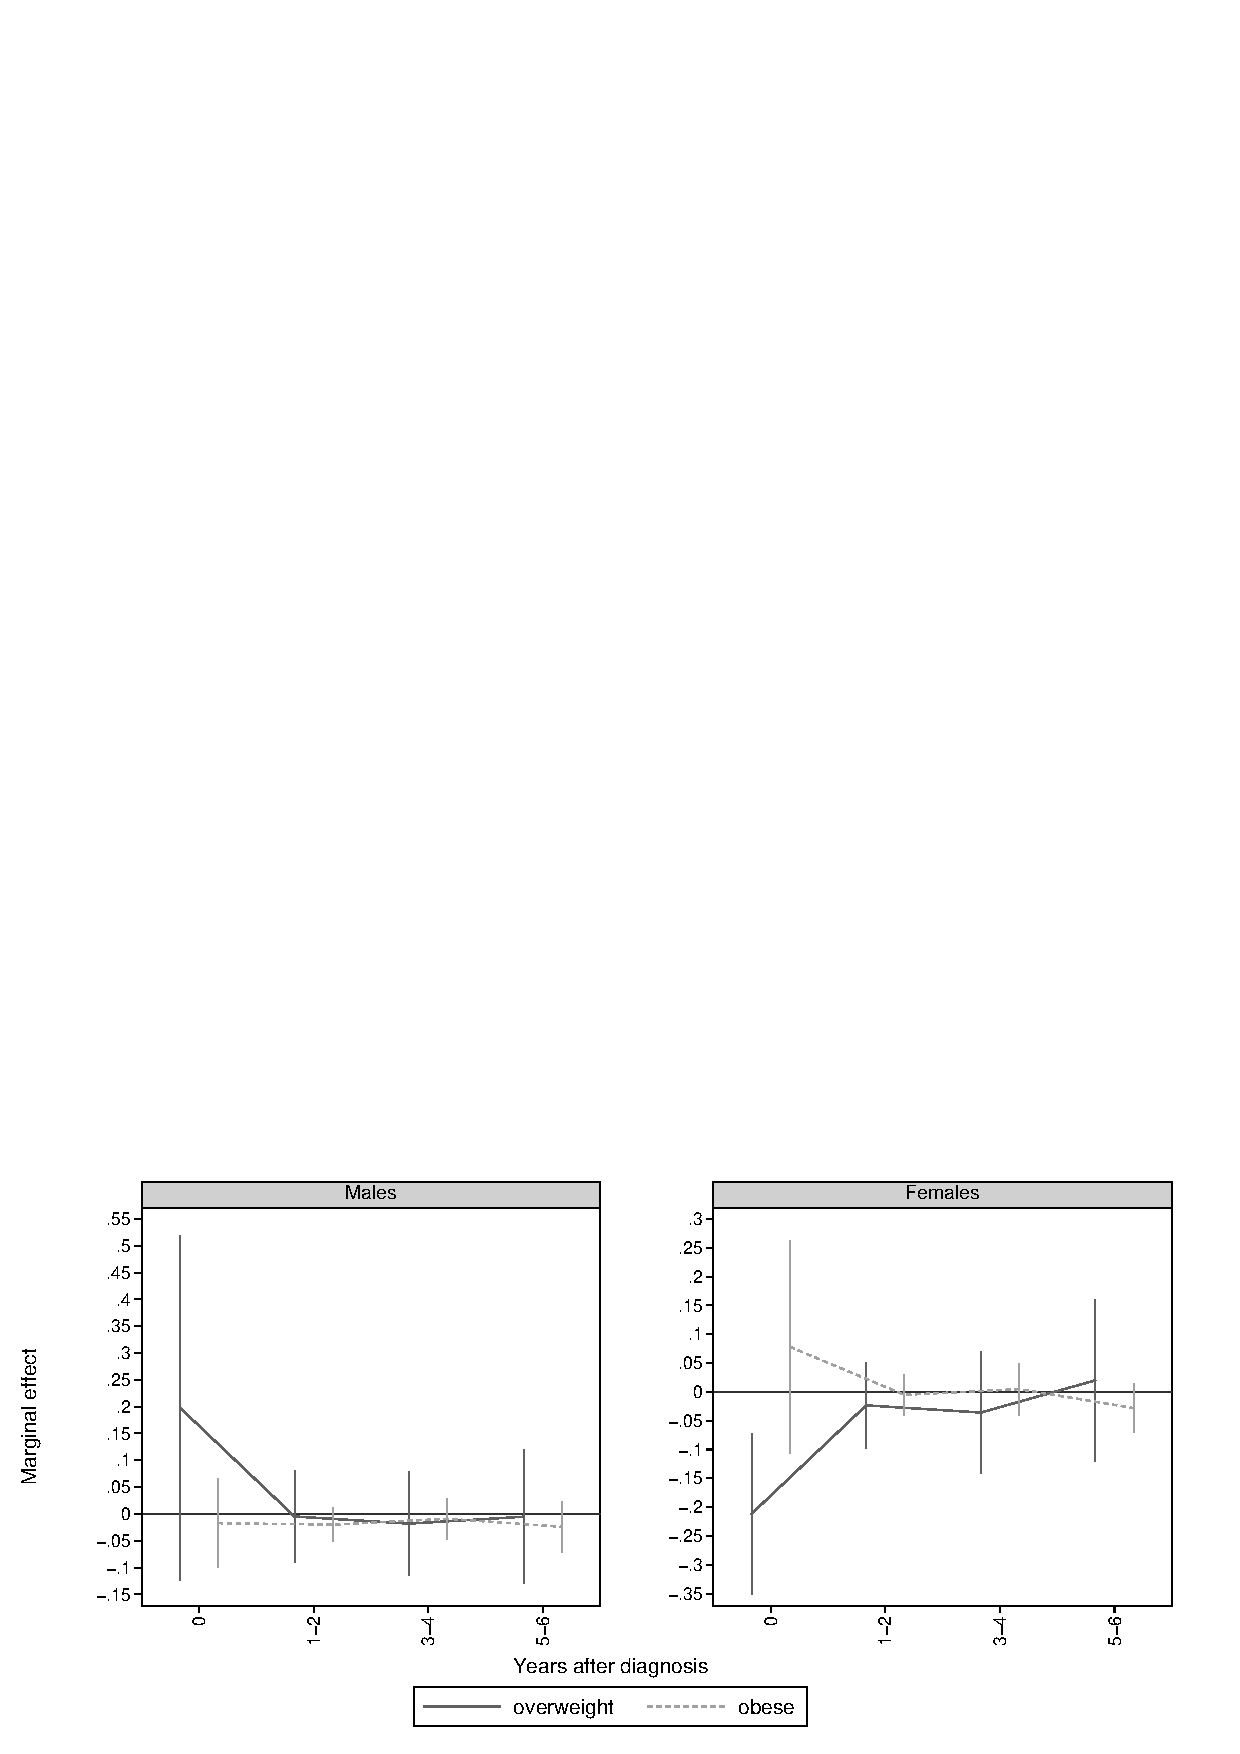
\includegraphics[width=\linewidth]{Chapter5/Figures/mi_msm_l_all_obese.pdf}
Fixed effects
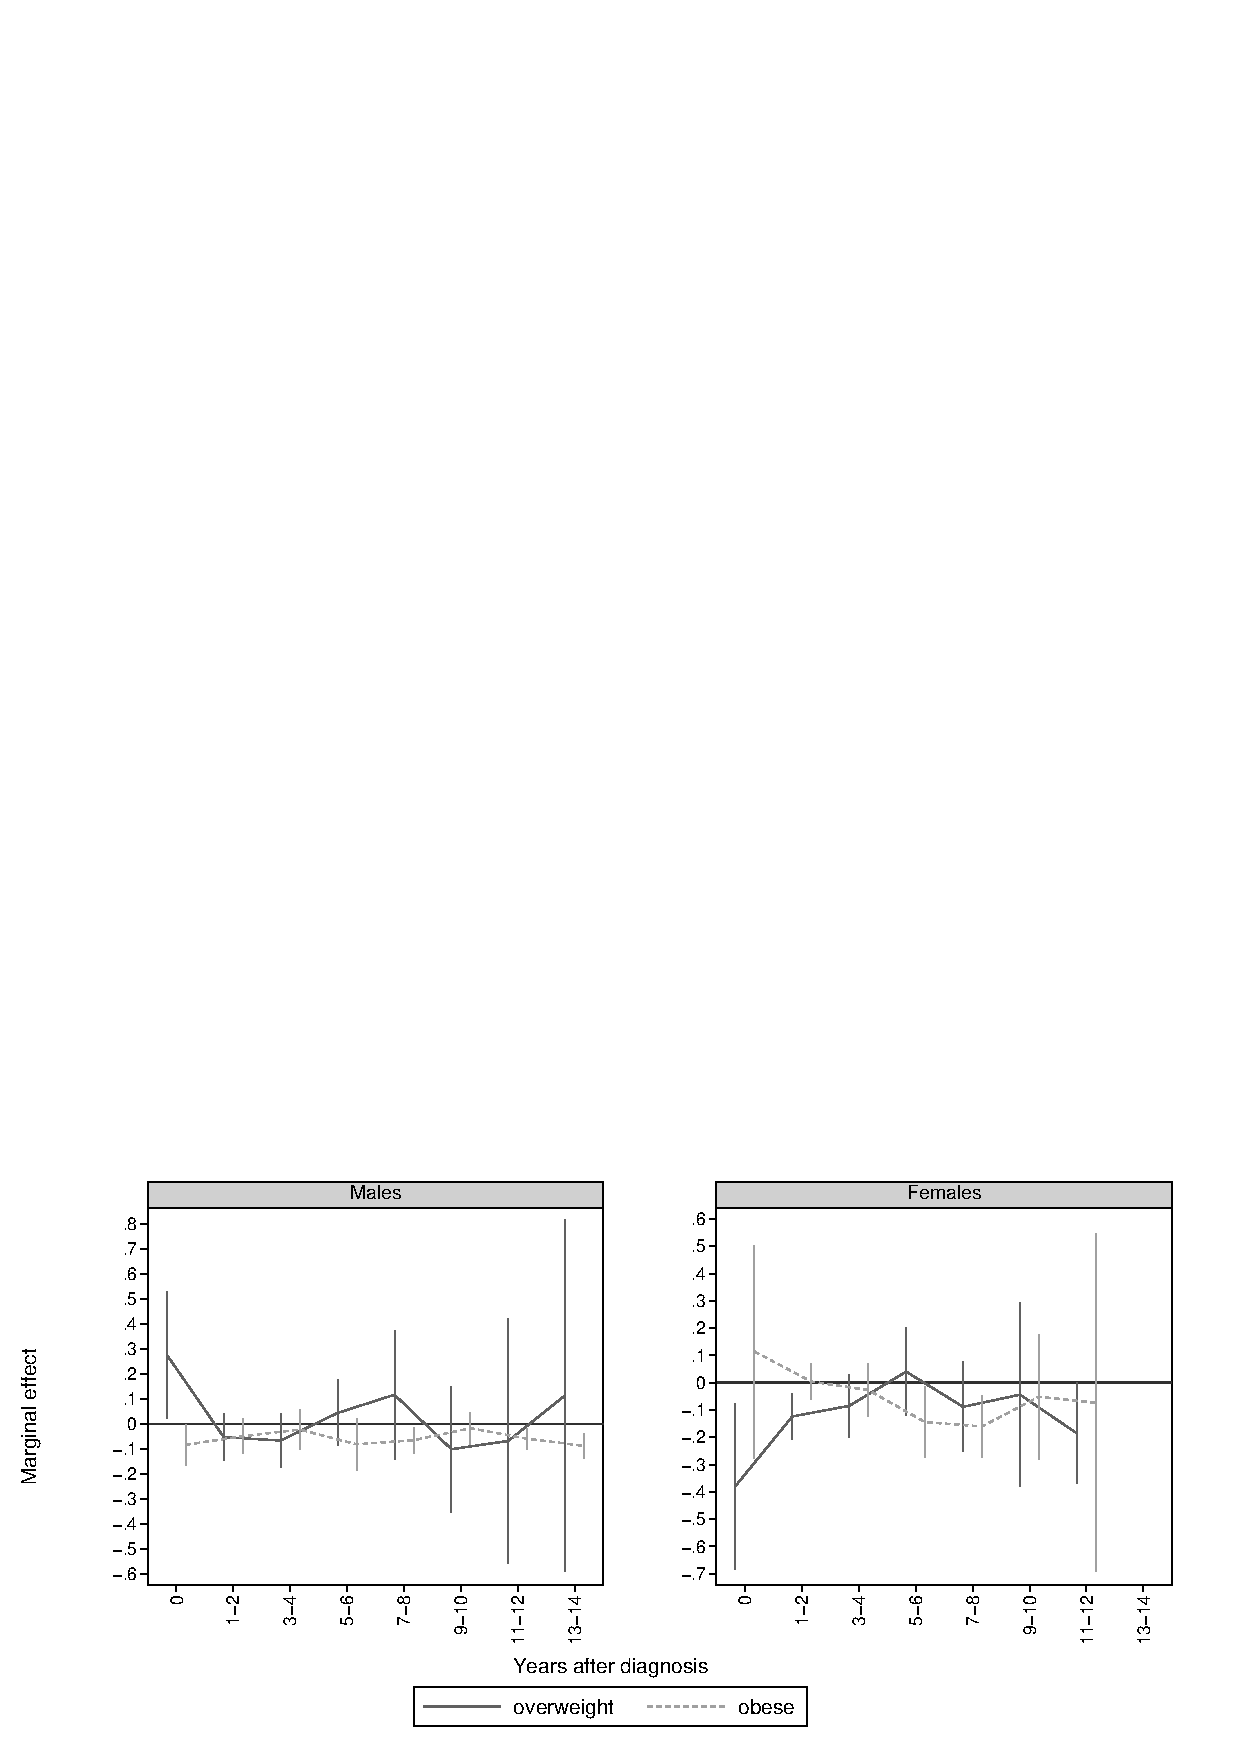
\includegraphics[width=\linewidth]{Chapter5/Figures/mi_obese_fe.pdf}
Random effects
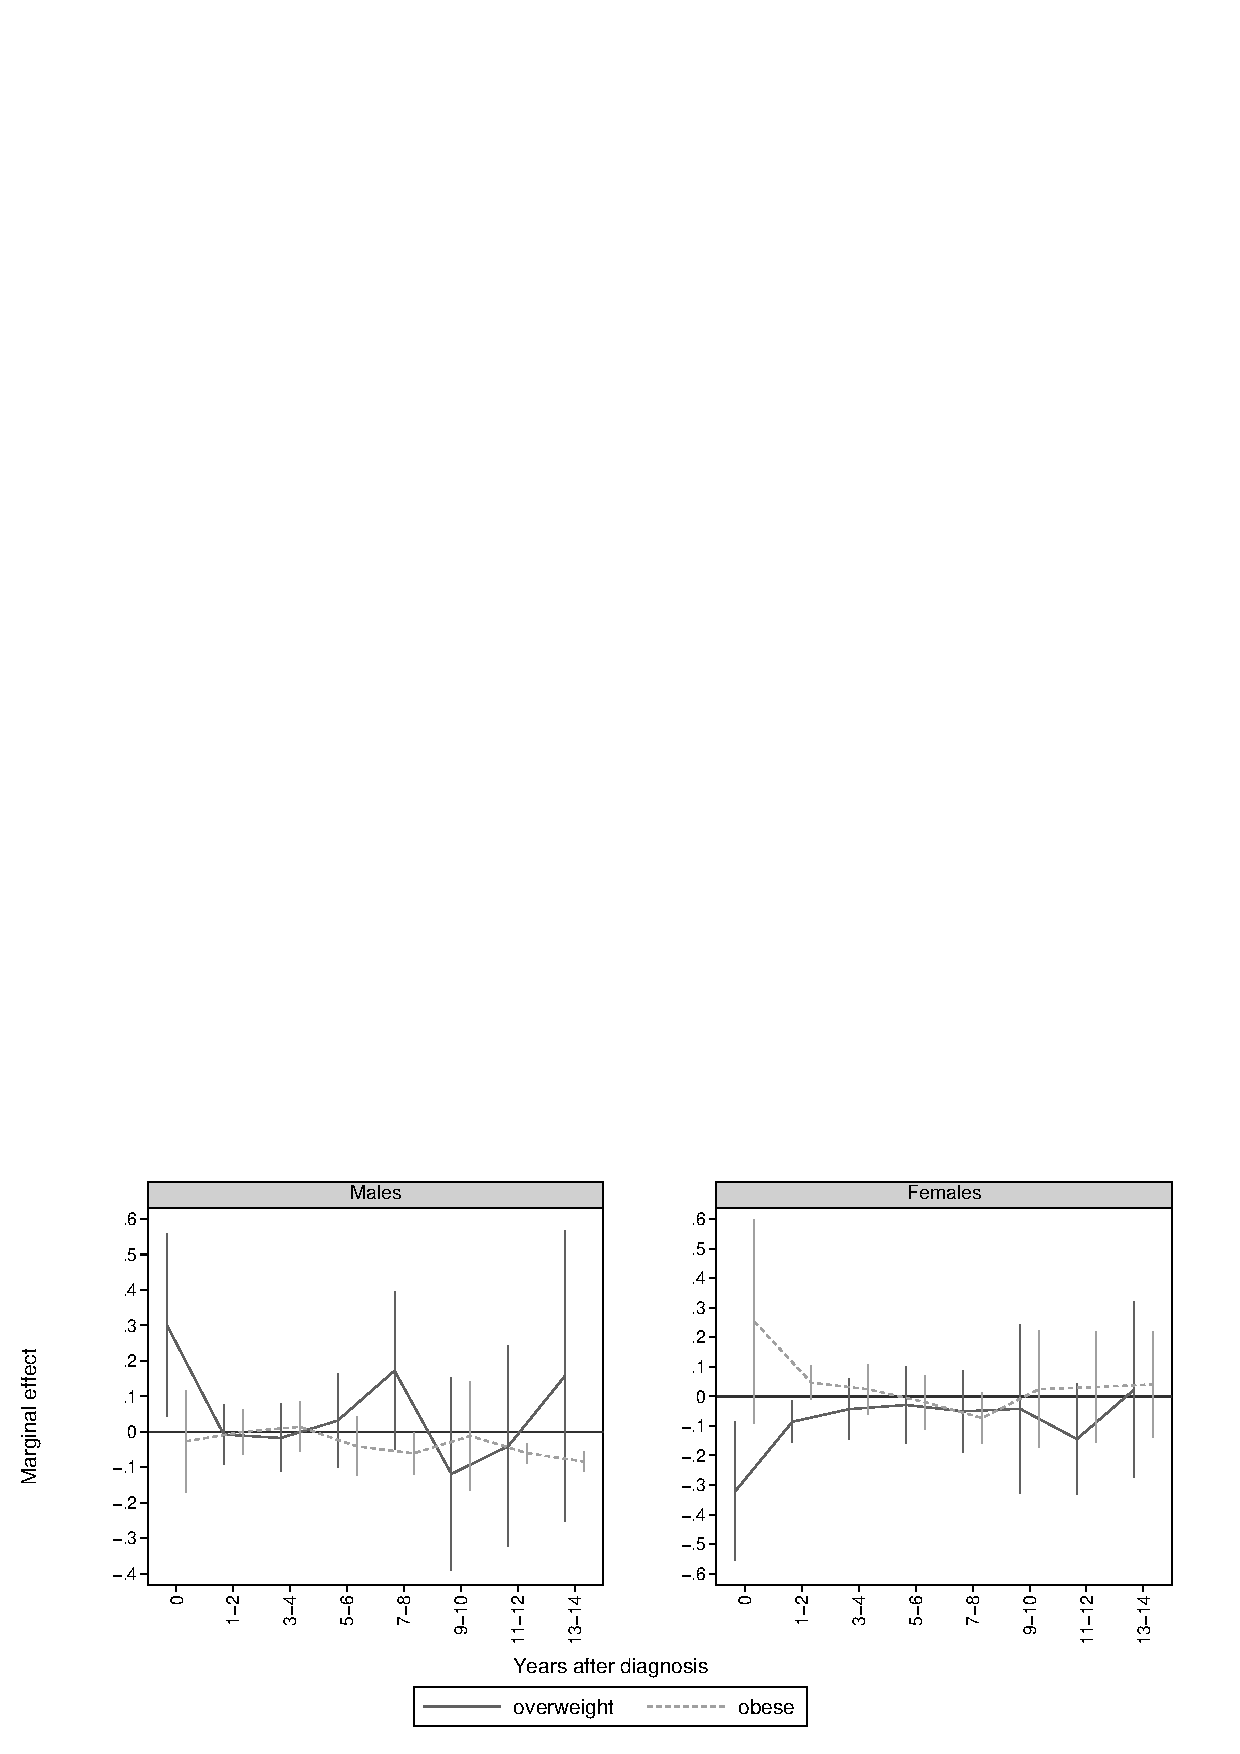
\includegraphics[width=\linewidth]{Chapter5/Figures/mi_obese_re.pdf}
\footnotetext{\textit{Notes} 95\% confidence intervals. Estimation only possible up to year 6 due to too few observations for estimation for the later groups}
\end{center}
\end{figure}
\clearpage \newpage 
%}
\cleardoublepage
\end{document}          
